% Options for packages loaded elsewhere
\PassOptionsToPackage{unicode}{hyperref}
\PassOptionsToPackage{hyphens}{url}
%
\documentclass[
]{book}
\usepackage{amsmath,amssymb}
\usepackage{lmodern}
\usepackage{ifxetex,ifluatex}
\ifnum 0\ifxetex 1\fi\ifluatex 1\fi=0 % if pdftex
  \usepackage[T1]{fontenc}
  \usepackage[utf8]{inputenc}
  \usepackage{textcomp} % provide euro and other symbols
\else % if luatex or xetex
  \usepackage{unicode-math}
  \defaultfontfeatures{Scale=MatchLowercase}
  \defaultfontfeatures[\rmfamily]{Ligatures=TeX,Scale=1}
\fi
% Use upquote if available, for straight quotes in verbatim environments
\IfFileExists{upquote.sty}{\usepackage{upquote}}{}
\IfFileExists{microtype.sty}{% use microtype if available
  \usepackage[]{microtype}
  \UseMicrotypeSet[protrusion]{basicmath} % disable protrusion for tt fonts
}{}
\makeatletter
\@ifundefined{KOMAClassName}{% if non-KOMA class
  \IfFileExists{parskip.sty}{%
    \usepackage{parskip}
  }{% else
    \setlength{\parindent}{0pt}
    \setlength{\parskip}{6pt plus 2pt minus 1pt}}
}{% if KOMA class
  \KOMAoptions{parskip=half}}
\makeatother
\usepackage{xcolor}
\IfFileExists{xurl.sty}{\usepackage{xurl}}{} % add URL line breaks if available
\IfFileExists{bookmark.sty}{\usepackage{bookmark}}{\usepackage{hyperref}}
\hypersetup{
  pdftitle={Análises Ecológicas no R},
  hidelinks,
  pdfcreator={LaTeX via pandoc}}
\urlstyle{same} % disable monospaced font for URLs
\usepackage{color}
\usepackage{fancyvrb}
\newcommand{\VerbBar}{|}
\newcommand{\VERB}{\Verb[commandchars=\\\{\}]}
\DefineVerbatimEnvironment{Highlighting}{Verbatim}{commandchars=\\\{\}}
% Add ',fontsize=\small' for more characters per line
\usepackage{framed}
\definecolor{shadecolor}{RGB}{248,248,248}
\newenvironment{Shaded}{\begin{snugshade}}{\end{snugshade}}
\newcommand{\AlertTok}[1]{\textcolor[rgb]{0.33,0.33,0.33}{#1}}
\newcommand{\AnnotationTok}[1]{\textcolor[rgb]{0.37,0.37,0.37}{\textbf{\textit{#1}}}}
\newcommand{\AttributeTok}[1]{\textcolor[rgb]{0.61,0.61,0.61}{#1}}
\newcommand{\BaseNTok}[1]{\textcolor[rgb]{0.06,0.06,0.06}{#1}}
\newcommand{\BuiltInTok}[1]{#1}
\newcommand{\CharTok}[1]{\textcolor[rgb]{0.5,0.5,0.5}{#1}}
\newcommand{\CommentTok}[1]{\textcolor[rgb]{0.37,0.37,0.37}{\textit{#1}}}
\newcommand{\CommentVarTok}[1]{\textcolor[rgb]{0.37,0.37,0.37}{\textbf{\textit{#1}}}}
\newcommand{\ConstantTok}[1]{\textcolor[rgb]{0,0,0}{#1}}
\newcommand{\ControlFlowTok}[1]{\textcolor[rgb]{0.27,0.27,0.27}{\textbf{#1}}}
\newcommand{\DataTypeTok}[1]{\textcolor[rgb]{0.27,0.27,0.27}{#1}}
\newcommand{\DecValTok}[1]{\textcolor[rgb]{0.06,0.06,0.06}{#1}}
\newcommand{\DocumentationTok}[1]{\textcolor[rgb]{0.37,0.37,0.37}{\textbf{\textit{#1}}}}
\newcommand{\ErrorTok}[1]{\textcolor[rgb]{0.14,0.14,0.14}{\textbf{#1}}}
\newcommand{\ExtensionTok}[1]{#1}
\newcommand{\FloatTok}[1]{\textcolor[rgb]{0.06,0.06,0.06}{#1}}
\newcommand{\FunctionTok}[1]{\textcolor[rgb]{0,0,0}{#1}}
\newcommand{\ImportTok}[1]{#1}
\newcommand{\InformationTok}[1]{\textcolor[rgb]{0.37,0.37,0.37}{\textbf{\textit{#1}}}}
\newcommand{\KeywordTok}[1]{\textcolor[rgb]{0.27,0.27,0.27}{\textbf{#1}}}
\newcommand{\NormalTok}[1]{#1}
\newcommand{\OperatorTok}[1]{\textcolor[rgb]{0.43,0.43,0.43}{\textbf{#1}}}
\newcommand{\OtherTok}[1]{\textcolor[rgb]{0.37,0.37,0.37}{#1}}
\newcommand{\PreprocessorTok}[1]{\textcolor[rgb]{0.37,0.37,0.37}{\textit{#1}}}
\newcommand{\RegionMarkerTok}[1]{#1}
\newcommand{\SpecialCharTok}[1]{\textcolor[rgb]{0,0,0}{#1}}
\newcommand{\SpecialStringTok}[1]{\textcolor[rgb]{0.5,0.5,0.5}{#1}}
\newcommand{\StringTok}[1]{\textcolor[rgb]{0.5,0.5,0.5}{#1}}
\newcommand{\VariableTok}[1]{\textcolor[rgb]{0,0,0}{#1}}
\newcommand{\VerbatimStringTok}[1]{\textcolor[rgb]{0.5,0.5,0.5}{#1}}
\newcommand{\WarningTok}[1]{\textcolor[rgb]{0.37,0.37,0.37}{\textbf{\textit{#1}}}}
\usepackage{longtable,booktabs,array}
\usepackage{calc} % for calculating minipage widths
% Correct order of tables after \paragraph or \subparagraph
\usepackage{etoolbox}
\makeatletter
\patchcmd\longtable{\par}{\if@noskipsec\mbox{}\fi\par}{}{}
\makeatother
% Allow footnotes in longtable head/foot
\IfFileExists{footnotehyper.sty}{\usepackage{footnotehyper}}{\usepackage{footnote}}
\makesavenoteenv{longtable}
\setlength{\emergencystretch}{3em} % prevent overfull lines
\providecommand{\tightlist}{%
  \setlength{\itemsep}{0pt}\setlength{\parskip}{0pt}}
\setcounter{secnumdepth}{5}
\usepackage{booktabs}
\usepackage{longtable}
\usepackage[bf,singlelinecheck=off]{caption}

\usepackage{Alegreya}
\usepackage[scale=.8]{sourcecodepro}

\usepackage{framed,color}
\definecolor{shadecolor}{RGB}{248,248,248}

\renewcommand{\textfraction}{0.05}
\renewcommand{\topfraction}{0.8}
\renewcommand{\bottomfraction}{0.8}
\renewcommand{\floatpagefraction}{0.75}

\renewenvironment{quote}{\begin{VF}}{\end{VF}}
\let\oldhref\href
\renewcommand{\href}[2]{#2\footnote{\url{#1}}}

\ifxetex
  \usepackage{letltxmacro}
  \setlength{\XeTeXLinkMargin}{1pt}
  \LetLtxMacro\SavedIncludeGraphics\includegraphics
  \def\includegraphics#1#{% #1 catches optional stuff (star/opt. arg.)
    \IncludeGraphicsAux{#1}%
  }%
  \newcommand*{\IncludeGraphicsAux}[2]{%
    \XeTeXLinkBox{%
      \SavedIncludeGraphics#1{#2}%
    }%
  }%
\fi

\usepackage{makeidx}
\makeindex

\urlstyle{tt}

\usepackage{amsthm}
\makeatletter
\def\thm@space@setup{%
  \thm@preskip=8pt plus 2pt minus 4pt
  \thm@postskip=\thm@preskip
}
\makeatother

\frontmatter
\ifluatex
  \usepackage{selnolig}  % disable illegal ligatures
\fi
\usepackage[]{natbib}
\bibliographystyle{apalike}

\title{Análises Ecológicas no R}
\author{}
\date{\vspace{-2.5em}2021-08-12}

\begin{document}
\maketitle

\cleardoublepage\newpage\thispagestyle{empty}\null
\cleardoublepage\newpage\thispagestyle{empty}\null
%\cleardoublepage\newpage
\thispagestyle{empty}
\begin{large}
To the most amazing cooks in my life, Xie Shaobai and Si Zhinan.
\begin{flushright}
---Yihui
\end{flushright}

\bigskip

To my supporting wife, Caroline, and our lovely newborn, Axel.
\begin{flushright}
---Christophe
\end{flushright}

\bigskip

To my mom, who taught me the joy of life-long learning.
\begin{flushright}
---Emily
\end{flushright}
\end{large}

\setlength{\abovedisplayskip}{-5pt}
\setlength{\abovedisplayshortskip}{-5pt}

{
\setcounter{tocdepth}{2}
\tableofcontents
}
\hypertarget{capa}{%
\chapter*{Capa}\label{capa}}


\newpage

\hypertarget{prefuxe1cio}{%
\chapter*{Prefácio}\label{prefuxe1cio}}


\newpage

\hypertarget{base-r}{%
\chapter{Pré-requisitos}\label{base-r}}

\hypertarget{introduuxe7uxe3o}{%
\section{Introdução}\label{introduuxe7uxe3o}}

O objetivo desta seção é

\hypertarget{pacotes}{%
\section{Pacotes}\label{pacotes}}

\hypertarget{versuxe3o-do-r}{%
\section{Versão do R}\label{versuxe3o-do-r}}

\hypertarget{dados}{%
\section{Dados}\label{dados}}

\hypertarget{cap2}{%
\chapter{Introdução}\label{cap2}}

\hypertarget{histuxf3rico-deste-livro}{%
\section{Histórico deste livro}\label{histuxf3rico-deste-livro}}

Este livro foi estruturado a partir da apostila elaborada pelos pesquisadores Diogo B. Provete, Fernando R. da Silva e Thiago Gonçalves-Souza para ministrar o curso \emph{Estatística aplicada à ecologia usando o R} no PPG em Biologia Animal da UNESP de São José Rio Preto/SP, em abril de 2011. Os três pesquisadores eram então alunos do PPG em Biologia Animal quando elaboraram o material disponibilizado na \href{(https://cran.r-project.org/doc/contrib/Provete-Estatistica_aplicada.pdf)}{apostila}. A proposta de transformar a apostila em livro sempre foi um tópico recorrente desde 2011, e concretizado agora, 10 anos depois.

Neste período, Diogo, Fernando e Thiago foram contratados pela Universidade Federal de Mato Grosso do Sul, Universidade Federal de São Carlos campus Sorocaba, e Universidade Federal Rural de Pernambuco, respectivamente. Nestes anos eles ofertaram diferentes versões do curso \emph{Estatística aplicada à ecologia usando o R} para alunos de graduação e pós-graduação em diferentes instituições do Brasil. A possibilidade da oferta destes novos cursos fortaleceu a ideia de trasformar a apostila em um livro com base nas experiências dos pesquisadores em sala de aula.

Considerando que novas abordagens ecológicas vêm sendo descritas e criadas a uma taxa elevada nos últimos anos, era de se esperar que as informações disponíveis na apostila estivessem defasadas após 10 anos. Por este motivo, Diogo, Fernando e Thiago convidaram outros dois pesquisadores, Gustavo B. Paterno da Georg-August-University of Göttingen e Maurício H. Vancine do PPG em Ecologia, Evolução e Biodiversidade da UNESP Câmpus de Rio Claro, que são referências no uso de estatística em ecologia usando o R. Com o time completo, passaram mais de um ano realizando reuniões, compartilhando scripts e pagando cerveja para os coautores por capítulos atrasados até chegarem neste primeira versão do livro.

\hypertarget{objetivo-deste-livro}{%
\section{Objetivo deste livro}\label{objetivo-deste-livro}}

Nossa proposta com este livro é de traçar o melhor caminho (pelo menos do nosso ponto de vista) entre questões ecológicas e os métodos estatísticos mais robustos para testá-las. Guiar seus passos nesse caminho (nem sempre linear) necessita que você utilize um requisito básico: o de utilizar seu esforço para caminhar. O nosso esforço, em contrapartida, será o de indicar as melhores direções para que você adquira certa independência em análises ecológicas. Um dos nossos objetivos é mostrar que o conhecimento de teorias ecológicas e a utilização de questões apropriadas são o primeiro passo na caminhada rumo à compreensão da lógica estatística. Não deixe que a estatística se torne a ``pedra no seu caminho''. Em nossa opinião, programas com ambiente de programação favorecem o entendimento da lógica estatística, uma vez que cada passo (lembre-se de que você está caminhado em uma estrada desconhecida e cheia de pedras) precisa ser coordenado, ou seja, as linhas de comando (detalhes abaixo) precisam ser compreendidas para que você teste suas hipóteses.

A primeira parte deste livro pretende utilizar uma estratégia que facilita a escolha do teste estatístico apropriado, por meio da seleção de questões/hipóteses claras e da ligação dessas hipóteses com a teoria e o método (veja Figura \ref{fig:fig-statistical-thinking} no Capítulo \ref{cap3}). Enfatizamos que é fundamental ter em mente aonde se quer chegar, para poder escolher o que deve ser feito. Posteriormente à escolha de suas questões, é necessário transferir o contexto ecológico para um contexto meramente estatístico (hipótese nula/alternativa). A partir da definição de uma hipótese nula, partiremos para a aplicação de cada teste estatístico (de modelos lineares generalizados à análises multivariadas) utilizando a linguagem R.

Antes de detalhar cada análise estatística, apresentaremos os comandos básicos para a utilização da linguagem R e os tipos de distribuição estatística que são essenciais para a compreensão dos testes estatísticos. Para isso, organizamos um esquema que chamamos de ``estrutura lógica'' que facilita a compreensão dos passos necessários para testar suas hipóteses (veja Figura \ref{fig:fig-box} no Capítulo \ref{cap3}).

\hypertarget{o-que-vocuxea-nuxe3o-encontraruxe1-neste-livro}{%
\section{O que você não encontrará neste livro}\label{o-que-vocuxea-nuxe3o-encontraruxe1-neste-livro}}

Aprofundamento teórico, detalhes matemáticos, e explicação dos algoritmos são informações que infelizmente não serão abordadas neste livro. O foco aqui é a explicação de como cada teste funciona (teoria e procedimentos matemáticos básicos) e sua aplicação em testes ecológicos usando scripts na linguagem R. Para tanto, o livro de Pierre e Louis Legendre \citep{legendre_numerical_2012} é uma leitura que permite o aprofundamento de cada uma das análises multivariadas propostas aqui. Além disso, são de fundamental importância para o amadurecimento em análises ecológicas as seguintes leituras: \citet{manly_randomization_1991}, \citet{pinheiro_mixed-effects_2000}, \citet{scheiner_design_2001}, \citet{burnham_pvalues_2014}, \citet{quinn_experimental_2002}, \citet{venables_modern_2002}, \citet{magurran_biological_2011}, \citet{gotelli_primer_2013}, \citet{zar_biostatistical_2010}, \citet{zuur_protocol_2009}, \citet{crawley_r_2012} e \citet{james_introduction_2013}.

\hypertarget{por-que-usar-o-r}{%
\section{Por que usar o R?}\label{por-que-usar-o-r}}

Os criadores do R o chamam de uma linguagem e ambiente de programação estatística e gráfica \citep{venables_modern_2002}. A linguagem R também é chamada de programação ``orientada ao objeto'' (\emph{object oriented programming}), o que significa que utilizar o R envolve basicamente a criação e manipulação de objetos em uma tela branca, em que o usuário tem de dizer exatamente o que deseja que o programa execute, ao invés de simplesmente clicar em botões. E vem daí uma das grandes vantagens em se usar o R: o usuário tem total controle sobre o que está acontecendo e também tem de compreender o que deseja antes de executar uma análise. Além disso, o R permite integração com outros programas escritos em C++, Python e Java, permitindo que os usuários possam aplicar novas metodologias sem ter que aprender novas linguagens.

Na página pessoal do Prof.~Nicolas J. Gotelli (\href{http://www.uvm.edu/~ngotelli/homepage.html}{link}), existem vários conselhos para um estudante iniciante de ecologia. Dentre esses conselhos, o Prof.~Gotelli menciona que o domínio de uma linguagem de programação é uma das habilidades mais importantes, porque dá liberdade ao ecólogo para executar tarefas que vão além daquelas disponíveis em pacotes estatísticos comerciais. Além disso, a maioria das novas análises propostas nos mais reconhecidos periódicos em ecologia normalmente são implementadas em linguagem R, e os autores incluem normalmente o código fonte no material suplementar dos artigos, tornando a análise acessível. A partir do momento que essas análises ficam disponíveis (seja por código fornecido pelo autor ou por implementação em pacotes pré-existentes), é mais simples entendermos a lógica de análises complexas, especialmente as multivariadas, utilizando nossos próprios dados, realizando-as passo a passo. Sem a utilização do R, normalmente temos que contatar os autores que nem sempre são tão acessíveis.

Uma última vantagem é que por ser um software livre, a citação do R em artigos é permitida e até aconselhável. Para saber como citar o R, digite \texttt{citation()} na linha de comando. Para citar um pacote específico, digite \texttt{citation()} com o nome do pacote entre aspas dentro dos parênteses. Neste ponto, esperamos ter convencido você leitor, de que aprender a utilizar o R tem inúmeras vantagens. Entretanto, provavelmente vai ser difícil no começo, mas continue e perceberá que o investimento vai valer à pena no futuro.

\hypertarget{indo-aluxe9m-da-linguagem-de-prograuxe7uxe3o-para-a-ecologia}{%
\section{Indo além da linguagem de progração para a Ecologia}\label{indo-aluxe9m-da-linguagem-de-prograuxe7uxe3o-para-a-ecologia}}

Um ponto em comum em que todos os autores deste livro concordaram em conversas durante sua estruturação, foi a dificuldade que todos tivemos quando estávamos aprendendo a linguagem:

\begin{quote}
\begin{enumerate}
\def\labelenumi{\arabic{enumi}.}
\tightlist
\item
  Como transcrever os objetivos (manipulação de dados, análises e gráficos) em linguagem R
\item
  Como interpretar os resultados das análises estatísticas do R para os objetivos ecológicos
\end{enumerate}
\end{quote}

Num primeiro momento, quando estamos aprendendo a linguagem R é muito desafiador pensar em como estruturar nossos códigos para que eles façam o que precisamos: importar dados, selecionar linhas ou colunas, qual pacote ou função usar para uma certa análise ou como fazer um gráfico que nas nossas anotações são simples, mas no código parece impossível. Bem, não há um caminho fácil nesse sentido e ele depende muito da experiência e familiaridade adquirida com o tempo de uso da linguagem, assim como outra língua qualquer, como inglês ou espanhol. Entretanto, uma dica pode ajudar: estruture seus códigos antes de partir para o R. Num papel escreva os pontos que quer que seus códigos façam, como se estivesse explicando para alguém os passos que precisa para realizar as tarefas. Depois disso, transcreva para o script (iremos explicar esse conceito no @{[}cap4{]}) esse texto. Por fim, traduza isso em linguam R. Pode parecer massante e cansativo no começo, mas isso o ajudará a ter maior domínio da linguagem, sendo que esse passo se torna desnecessário quando se adquire bastante experiência.

Uma vez transposta esse barreira inicial e temos os resultados de nossas análises (valores de estatísticas, parâmetros estimados, valores de p e R², etc.), com gráficos e outras figuras que precisamos, como interpretamos à luz da teoria ecológica? Esse ponto é talvez um dos mais complicados. Com o tempo, ter um valor final de uma estatística ou gráfico à partir da linaguagem R é relativamente simples, mas o que esse valor ou gráfico significam para nossa hipótese ecológica é o ponto mais complicado. Essa dificuldade por ser por inexperiência teórica (ainda não lemos muito sobre um aspecto ecológico) ou inexperiência científica (ainda temos dificuldade para expandir nossos argumentos de forma indutiva). Destacamos esse ponto porque ele é fundamental no processo científico e talvez seja o principal aspecto que diferencia os cientistas de outros profissionais: sua capacidade de entendimento dos padrões à partir dos processos e mecanismos atrelados. Nesse ponto, quase sempre recorremos à nossos orientadores ou colegas mais experientes para nos ajudar, mas é natural e faz parte do processo de aprendizado de uso da linguagem R junto à Ecologia como ciência. Entretanto, contrapomos a importância dessa extrapolação para não nos tornarmos apenas especialistas em linguagem R sem a fundamental capacidade de entendimento do sistema ecológico que estamos estudando.

\hypertarget{como-usar-este-livro}{%
\section{Como usar este livro}\label{como-usar-este-livro}}

Os conteúdos apresentados em cada capítulo são independentes entre si. Portanto, você pode utilizar este livro de duas formas. A primeira é seguir uma ordem sequencial (capítulos 1, 2, 3, \ldots) que recomendamos, principalmente, para as pessoas que não possuem familiaridade com a linguagem R. A segunda forma, é selecionar o capítulo que contém a análise de seu interesse e mudar de um capítulo para outro sem seguir a sequência apresentada no livro.

Com exceção dos capítulos 3, 4, 5 e 15, os outros capítulos foram elaborados seguindo a mesma estrutura contendo uma descrição da análise estatística (aspecto teóricos) e exemplos relacionados com questões ecólogicas que podem ser respondidas por esta análise. Todos os exemplos são compostos por: i) uma descrição dos dados utilizados, ii) pergunta e predição do trabalho, iii) descrição das variáveis resposta(s) e preditora(s), e iv) descrição e explicação das linhas de comando do R necessárias para realização das análises. Os exemplos utilizados são baseados em dados reais que já foram publicados em artigos científicos ou são dados coletados por um dos autores deste livro. Nós recomendamos que primeiro você utilize estes exemplos para se familiarizar com as análises e a formatação das linhas e colunas das planilhas. Em seguida, utilize seus próprios dados para realizar as análises. Esta é a melhor maneira de se familiarizar com as linhas de comando do R.

Muitas das métricas ou índices apresentados neste livro não foram traduzidas para o português, porque seus acrônimos são clássicos e bem estabelecidos na literatura ecológica. Nestes casos, consideramos que a tradução poderia confundir as pessoas que estão começando a se familiarizar com a literatura específica. Realçamos que não estamos abordando todas as possibilidades disponíveis, e existem muito outros pacotes e funções no R que realizam as mesmas análises. Contudo, esperamos que o conteúdo apresentado permita que os leitores adquiram independência e segurança, para que possam caminhar sozinhos na exploração de novos pacotes e funções para responderem suas perguntas biológicas e ecológicas.

\hypertarget{cap3}{%
\chapter{Voltando ao básico: como dominar a arte de fazer perguntas cientificamente relevantes}\label{cap3}}

\emph{Capítulo originalmente publicado por Gonçalves-Souza, Provete, Garey, Silva \& Albuquerque \citeyearpar{albuquerque_going_2019}, in Methods and Techniques in Ethnobiology and Ethnoecology (tradução autorizada por Springer).}

\hypertarget{introduuxe7uxe3o-1}{%
\section{Introdução}\label{introduuxe7uxe3o-1}}

\begin{quote}
\emph{Aquele que ama a prática sem teoria é como um marinheiro que embarca em um barco sem um leme e uma bússola e nunca sabe onde pode atracar - Leonardo da Vinci.}
\end{quote}

Qual é a sua pergunta? Talvez esta seja a frase que pesquisadores mais jovens ouvem quando começam suas atividades científicas. Apesar de aparentemente simples, responder a esta pergunta se torna um dos maiores desafios da formação científica. Seja na pesquisa quantitativa ou qualitativa, todo processo de busca de conhecimento parte de uma questão/problema formulada pelo pesquisador no início desse processo. Esta questão guiará o pesquisador em todas as etapas da pesquisa. No caso específico de pesquisa quantitativa, a questão é a porta de entrada de uma das formas mais poderosas de pensar cientificamente: o método hipotético-dedutivo (MHD) definido por Karl Popper \citeyearpar{popper_logic_1959}. Este capítulo propõe uma maneira de pensar sobre hipóteses (geradas dentro do MHD) para melhorar o pensamento estatístico usando um fluxograma que relaciona variáveis por ligações causais. Além disso, argumentamos que você pode facilmente usar fluxogramas para (1) identificar variáveis relevantes e como elas afetam umas às outras; (2) melhorar (quando necessário) o desenho experimental/observacional; (3) facilitar a escolha de análises estatísticas; e (4) melhorar a interpretação e comunicação dos dados e análises.

\hypertarget{perguntas-devem-preceder-as-anuxe1lises-estatuxedsticas}{%
\section{Perguntas devem preceder as análises estatísticas}\label{perguntas-devem-preceder-as-anuxe1lises-estatuxedsticas}}

\hypertarget{um-bestiuxe1rio1-para-o-teste-de-hipuxf3teses-vocuxea-estuxe1-fazendo-a-pergunta-certa}{%
\subsection[Um bestiário para o teste de hipóteses (Você está fazendo a pergunta certa?)]{\texorpdfstring{Um bestiário\footnote{O bestiário é uma literatura do Século XII que descrevia animais (reais ou imaginários) com uma visão divertida e fantasiosa. Parte da interpretação continha lições de moral dos monges católicos que escreviam e ilustravam os bestiários. Longe de ser uma lição de moral ou mesmo uma descrição fantasiosa, usamos o termo bestiário neste livro para expressar o que há de mais importante e fantástico (na visão dos autores) para fazer um bom teste de hipóteses.} para o teste de hipóteses (Você está fazendo a pergunta certa?)}{Um bestiário para o teste de hipóteses (Você está fazendo a pergunta certa?)}}\label{um-bestiuxe1rio1-para-o-teste-de-hipuxf3teses-vocuxea-estuxe1-fazendo-a-pergunta-certa}}

A maioria dos alunos e professores de ciências biológicas possuem aversão à palavra ``estatística''. Não surpreendentemente, enquanto a maioria das disciplinas acadêmicas que compõem o ``STEM'' (termo em inglês para aglomerar \emph{Ciência, Tecnologia, Engenharia e Matemática}) têm uma sólida formação estatística durante a graduação, cursos de ciências biológicas têm um currículo fraco ao integrar o pensamento estatístico dentro de um contexto biológico \citep{metz_teaching_2008}. Esses cursos têm sido frequentemente ministrados sem qualquer abordagem prática para integrar os alunos em uma plataforma de solução de problemas \citep{horgan_teaching_1999}. Infelizmente, a Etnobiologia, Ecologia e Conservação (daqui em diante EEC) não são exceções. Talvez mais importante, uma grande preocupação durante o treinamento estatístico de estudantes de EEC é a necessidade de trabalhar com problemas complexos e multidemensionais que exigem soluções analíticas ainda mais complicadas para um público sem experiência em estatística e matemática. Por este motivo, muitos pesquisadores consideram a estatística como a parte mais problemática de sua pesquisa científica. Argumentamos neste capítulo que a dificuldade de usar estatística em EEC está associada à ausência de uma plataforma de solução de problemas gerando hipóteses claras que são derivadas de uma teoria. No entanto, concordamos que há um grande desafio em algumas disciplinas como a Etnobiologia para integrar esta abordagem direcionada por hipóteses, uma vez que foi introduzida apenas recentemente {[}veja \citet{phillips_useful_1993}; phillips\_useful\_1993-1; \citet{albuquerque_five_2009}{]}. Devido à falta de uma plataforma de solução de problemas, frequentemente percebemos que alunos/pesquisadores na EEC geralmente têm dificuldades de responder perguntas básicas para uma pesquisa científica, tais como:

\begin{enumerate}
\def\labelenumi{\arabic{enumi}.}
\tightlist
\item
  Qual é a principal teoria ou raciocínio lógico do seu estudo?
\item
  Qual é a questão principal do seu estudo?
\item
  Qual é a sua hipótese? Quais são suas predições?
\item
  Qual é a unidade amostral, variável independente e dependente de seu trabalho? Existe alguma covariável?
\item
  Qual é o grupo controle?
\end{enumerate}

Como selecionar qualquer teste estatístico sem responder a essas cinco perguntas? A estrutura estatística frequentista fornece uma maneira de ir progressivamente suportando ou falseando uma hipótese \citep{neyman__problem_1933, popper_logic_1959}. A decisão de rejeitar uma hipótese nula é feita usando um valor de probabilidade (geralmente P \textless{} 0,05) calculado pela comparação de eventos observados com observações repetidas obtidas a partir de uma distribuição nula.

Agora, vamos ensinar através de um exemplo e apresentar um ``guia para o pensamento estatístico'' que conecta alguns elementos essenciais para executar qualquer análise multivariada (ou univariada) \citep[Fig. \ref{fig:fig-statistical-thinking}, veja também a Fig. 1.3 em][ e Fig. 1 em \citet{underwood_experiments_1997}]{legendre_numerical_2012}. Primeiro, imagine que você observou os seguintes fenômenos na natureza: (1) ``indivíduos de uma população tradicional selecionar algumas plantas para fins médicos'' e (2)``manchas monodominantes da árvore \emph{Prosopis juliflora}, uma espécie invasora em várias regiões''. Do lado da etnobiologia, para entender como e porque o conhecimento tradicional é construído, existe uma teoria ou hipótese \citep[por exemplo, hipótese de aparência:][]{goncalves_most_2016} explicando os principais processos que ditam a seleção da planta (Fig. \ref{fig:fig-statistical-thinking}a).Então, você pode fazer uma ou mais perguntas relacionadas àquele fenômeno observado (Fig. \ref{fig:fig-statistical-thinking}b). Por exemplo, como a urbanização afeta o conhecimento das pessoas sobre o uso de plantas medicinais em diferentes biomas? Do lado ecológico/conservação, para entender por que espécies introduzidas afetam as espécies nativas locais, você precisa entender as teorias do nicho ecológico e evolutiva \citep{macdougall_plant_2009, saul_eco-evolutionary_2015}. Você pode perguntar, por exemplo, como as plantas exóticas afetam a estrutura de comunidades de plantas nativas? Questões complexas ou vagas dificultam a construção do fluxograma de pesquisa (ver descrição abaixo) e a seleção de testes estatísticos. Em vez disso, uma pergunta útil deve indicar as variáveis relevantes do seu estudo, como as independentes e dependentes, covariáveis, unidade de amostral e a escala espacial de interesse (Fig. \ref{fig:fig-statistical-thinking}b). No exemplo etnobiológico fornecido, a urbanização e o conhecimento das pessoas são as variáveis independentes e dependentes, respectivamente. Além disso, este estudo tem uma escala ampla, pois compara biomas diferentes. A próxima etapa é construir a hipótese biológica (Fig. \ref{fig:fig-statistical-thinking}c), que indicará a associação entre variáveis independentes e dependentes. No exemplo etnobiológico, a hipótese é que (1) ``a urbanização afeta o conhecimento das pessoas sobre o uso de plantas medicinais'', enquanto a hipótese ecológica é que (2) ``espécies exóticas afetam a estrutura de comunidades de plantas nativas''. Observe que isso é muito semelhante à questão principal. Mas você pode ter múltiplas hipóteses \citep{platt_strong_1964} derivado de uma teoria. Depois de selecionar a hipótese biológica (ou científica), é hora de pensar sobre a derivação lógica da hipótese, que é chamada de predição ou previsão (Fig. \ref{fig:fig-statistical-thinking}d). Os padrões preditos são uma etapa muito importante, pois após defini-los você pode operacionalizar suas variáveis e visualizar seus dados. Por exemplo, a variável teórica ``Urbanização'' pode ser medida como ``grau de urbanização ao longo das áreas urbanas, periurbanas e rurais'' e ``conhecimento das pessoas'' como ``o número e tipo de espécies de plantas úteis usadas para diferentes doenças''. Assim, a predição é que o grau de urbanização diminua o número e tipo de espécies de plantas conhecidas utilizadas para fins medicinais. No exemplo ecológico, a variável ``espécies exóticas'' pode ser medida como ``a densidade da planta exótica \emph{Prosopis juliflora}'' e ``Estrutura da comunidade'' como ``riqueza e composição de espécies nativas''. Depois de operacionalizar o seu trabalho à luz do método hipotético-dedutivo (HDM), o próximo passo é ``pensar estatisticamente'' sobre a hipótese biológica formulada (ver Figura \ref{fig:fig-statistical-thinking} e, f).

\begin{figure}

{\centering \includegraphics[width=0.7\linewidth]{img/cap03_fig01} 

}

\caption{Um guia para o pensamento estatístico combinando o método hipotético-dedutivo (a -- d, i) e estatística frequentista (e -- i). Veja também a Fig. 1 em Underwood 1997, Fig. 1 em Ford 2004 e Fig. 1.3 em Legendre & Legendre 2012.}\label{fig:fig-statistical-thinking}
\end{figure}

Então, você precisa definir as hipótese estatística nula (H0) e a alternativa (H1). Duas ``hipóteses estatísticas'' diferentes podem ser derivadas de uma hipótese biológica (Fig. \ref{fig:fig-statistical-thinking}e). Portanto, nós usamos o termo ``hipótese estatística'' entre aspas, porque as chamadas hipóteses estatísticas são predições \emph{sensu stricto}, e muitas vezes confundem jovens estudantes. A hipótese estatística nula representa uma ausência de relacão entre as variáveis independentese e dependentes. Depois de definir a hipótese estatística nula, você pode derivar uma ou várias hipóteses estatísticas alternativas, que demonstram a(s) associação(ões) esperada(s) entre suas variáveis (Fig. \ref{fig:fig-statistical-thinking}e). Em nosso exemplo, a hipótese nula é que ``o grau de urbanização não afeta o número de espécies de plantas úteis conhecidas pela população local''. Por sua vez, a hipótese alternativa é que ``o grau de urbanização afeta o número de espécies de plantas úteis conhecidas pela população local''. Depois de operacionalizar suas variáveis e definir o valor nulo e hipóteses alternativas, é hora de visualizar o resultado esperado (Fig. \ref{fig:fig-box}, Caixa 1) e escolher um método estatístico adequado. Por exemplo, se você deseja comparar a diferença na composição de plantas úteis entre áreas urbanas, periurbanas e rurais, você pode executar uma PERMANOVA \citep{albuquerque_multidimensional_2019} que usa uma estatística de teste chamada \emph{pseudo-F}. Então, você deve escolher o limite de probabilidade (o valor P) do teste estatístico para decidir se a hipótese nula deve ou não deve ser rejeitada \citep{gotelli_primer_2012}. Se você encontrar um P \textless{} 0,05, você deve rejeitar a hipótese estatística nula (urbanização não afeta o número e a composição das plantas). Por outro lado, um P \textgreater{} 0,05 indica que você não pode rejeitar a hipótese nula estatística. Assim, a estatística do teste e o valor P representam a última parte do teste de hipótese estatística, que é a decisão e conclusões apropriadas que serão usadas para retroalimentar a teoria principal (Figura \ref{fig:fig-statistical-thinking}g -- i). Generalizando seus resultados e falseando (ou não) suas hipóteses, o estudo busca refinar a construção conceitual da teoria, que muda constantemente \citep[Fig. 1i,][]{ford_scientific_2004}. No entanto, há um ponto crítico nesta última frase, porque a significância estatística não significa necessariamente relevância biológica \citep[ver discussão em][ e \citet{martinez-abrain_statistical_2008}]{gotelli_primer_2012}. Nas palavras de Ford (2004): ``as estatísticas são usadas para iluminar o problema, e não para apoiar uma posição''. Além disso, o procedimento de teste de hipótese tem alguma incerteza, que pode influenciar resultados ``falso-positivos'' (erro tipo 1) e ``falso-negativos'' (erro tipo 2) \citep{whitlock_analysis_2015}. Para simplificar, não discutiremos em detalhes os prós e contras da estatística frequentista, bem como métodos alternativos (por exemplo, Bayesiano e Máxima Verossimilhança), e questões filosóficas relativas ao ``valor P'' \citep[para uma discussão sobre esses tópicos, consulte o fórum em][]{ellison_p_2014}.

\begin{quote}
\textbf{Caixa 1. Tipo de variáveis e visualização de dados} Conforme descrito na Seção 3, o fluxograma é essencial para conectar variáveis relevantes para a pesquisa. Para aproveitar ao máximo esta abordagem, você pode desenhar suas próprias predições gráficas para te ajudar a pensar sobre diferentes possibilidades analíticas. Aqui, nós fornecemos uma descrição completa dos tipos de variáveis que você deve saber antes de executar qualquer análise estatística e representar seus resultados. Além disso, mostramos uma breve galeria (Fig. \ref{fig:fig-box}) com exemplos de boas práticas em visualização de dados \citep[Fig. \ref{fig:fig-research-flowchart}b, veja também figuras em][]{albuquerque_multidimensional_2019}. Além de conectar diferentes variáveis no fluxograma, você deve distinguir o tipo de variável. Primeiro você deve identificar as variáveis independentes (também conhecidos como explicativas ou preditoras) e dependentes (também conhecidas como resposta). A variável independente é aquela (ou aquelas) que prevê ou afeta a variável resposta (por exemplo, a fertilidade do solo é a variável independente capaz de afetar a abundância de uma espécie de planta focal, a variável dependente). Além disso, uma covariável é uma variável contínua que pode afetar tanto a variável resposta quanto a independente (ou ambos), mas geralmente não é do interesse do pesquisador. Depois de definir as variáveis relevantes, conectando-as no fluxograma, é hora de diferenciar seu tipo: (1) quantitativa ou contínua, e (2) categórica ou qualitativa (Fig. \ref{fig:fig-box}a, Caixa 1). O tipo de variável irá definir que tipo de figura você pode selecionar. Por exemplo, se você está comparando duas variáveis contínuas ou uma variável contínua e uma binária, a melhor maneira de visualizá-los (Fig. \ref{fig:fig-box}b) é um gráfico de dispersão (Fig. \ref{fig:fig-box}c, d). A linha representa os valores preditos pelo modelo estatístico usado (por exemplo, linear, logístico). Se você está interessado em comparar a gama de diferentes atributos (ou a descrição de qualquer variável numérica) entre as variáveis categóricas (por exemplo, espécies ou populações locais), um gráfico de halteres (do inglês Dumbbell plot) é uma boa opção (Fig. \ref{fig:fig-box}e). Histogramas também podem ser usados para mostrar a distribuição de duas variáveis contínuas de dois grupos ou fatores (Fig. \ref{fig:fig-box}f). No entanto, se você quiser testar o efeito de uma variável categórica independente (como em um desenho de ANOVA) sobre uma variável dependente, boxplots (Fig. \ref{fig:fig-box}g) ou gráficos de violino podem resumir essas relações de maneira elegante. Conjuntos de dados multivariados, por sua vez, podem ser visualizados com ordenação (Fig. \ref{fig:fig-box}h) ou gráficos de agrupamento (não mostrados). Existe um site abrangente apresentando várias maneiras de visualizar dados chamado \url{https://www.datavizproject.com/}.
\end{quote}

\begin{figure}

{\centering \includegraphics[width=1\linewidth]{img/cap03_fig02} 

}

\caption{(A) Tipos de variáveis e (B) visualização de dados para representar a relação entre variáveis independentes e dependentes ou covariáveis.}\label{fig:fig-box}
\end{figure}

\hypertarget{fluxograma-conectando-variuxe1veis-para-melhorar-o-desenho-experimental-e-as-anuxe1lises-estatuxedsticas}{%
\section{Fluxograma: Conectando Variáveis para Melhorar o desenho experimental e as análises estatísticas}\label{fluxograma-conectando-variuxe1veis-para-melhorar-o-desenho-experimental-e-as-anuxe1lises-estatuxedsticas}}

McIntosh e Pontius \citeyearpar{mcintosh_science_2017} afirmaram que o pensamento estatístico (representado na Fig. \ref{fig:fig-statistical-thinking} inclui quatro etapas importantes: (1) quais perguntas você investigaria (Seção 4), (2) como e onde coletar os dados \citep{ruxton_experimental_2016}, (3) quais fatores devem ser considerados e como eles afetam suas variáveis de interesse (e como elas afetam umas às outras), e (4) qual análise estatística você deve usar e como interpretar e comunicar os resultados (Seção 4). No entanto, a etapa (3) deve ser feita antes de coletar os dados. Por exemplo, se você está interessado na investigação dos benefícios das matas ciliares para as espécies nativas de peixes, quais variáveis devem ser incluídas no estudo? Se você escolher rios com e sem mata ciliar como única variável preditora, seu projeto de amostragem irá omitir outras variáveis de confusão, como ordem do rio e carbono orgânico do solo a montante. Vellend \citeyearpar{vellend_theory_2016} nomeou este problema como o ``problema de três caixas'' \citep[ver também][]{ruxton_experimental_2016} , que se refere à limitação em inferir que X (variável independente) causa variação em Y (variável depende) quando outras variáveis criam ou ampliam a correlação entre X e Y \citep[ver Fig. 2 em][]{ruxton_experimental_2016}. Uma ferramenta útil para compreender a relação entre todas as variáveis relevantes do seu estudo é um fluxograma. No ``fluxograma de pesquisa'' {[}ver também magnusson\_statistics\_2015{]} proposto aqui, variáveis dependentes (também conhecidas como resposta) e independentes (ou preditora), bem como covariáveis são representadas como caixas (com formas distintas: Fig. \ref{fig:fig-research-flowchart}). Além disso, você pode usar uma seta para representar uma (possível) via causal indicando força e sinal (positivo ou negativo) da variável preditora na variável dependente (Fig. \ref{fig:fig-research-flowchart}) Ao fazer isso, você pode melhorar o desenho experimental ou observacional incluindo ou controlando variáveis de confusão o que, por sua vez, pode ajudar a separar a contribuição relativa de diferentes variáveis preditoras em seu sistema. Mais importante, fazer conexões entre variáveis melhora sua capacidade de visualizar o ``Quadro geral'' de sua pesquisa, o que pode afetar seu experimento, análise estatística e revisão da literatura. Na verdade, Arlidge et al. \citeyearpar{arlidge_using_2017}argumentam que fluxogramas facilitam a construção de narrativas, melhorando: (1) a definição de múltiplas hipóteses, (2) coleta, interpretação e disseminação de dados e (3) a comunicação do conteúdo do estudo. Você também pode ler o livro de Magnusson et al. \citeyearpar{magnusson_statistics_2015} para entender mais como usar fluxogramas para auxiliar análises estatísticas. Além disso, Ford \citeyearpar{ford_scientific_2004} recomenda o uso de uma abordagem analítica para fomentar o desenvolvimento da pesquisa. Além disso, o fluxograma de pesquisa pode ser usado como uma ferramenta forte para contemplar os conselhos de Ford \citeyearpar{ford_scientific_2004}, que foram: (1) definir a pergunta da pesquisa, (2) definir a teoria a ser usada, (3) definir a técnica de investigação (por exemplo, experimento, observação de campo), (4) definir as medições, (5) definir como fazer inferência, e (6) interpretar, generalizar,e sintetizar a partir de dados que, por sua vez, são usados para refinar a teoria e modificar (quando necessário) questões futuras (Fig. \ref{fig:fig-statistical-thinking}).

\begin{figure}

{\centering \includegraphics[width=1\linewidth]{img/cap03_fig03} 

}

\caption{Exemplo de como usar um fluxograma para melhorar o entendimento do sistema estudado. A pergunta teórica "Qual é o impacto da invasão na comunidade nativa e nas propriedades do ecossistema?" pode gerar duas predições: (1) a planta exótica *Prosopis juliflora* reduz a diversidade beta de comunidades de plantas nativas, e (2) *Prosopis juliflora* modifica a composição das comunidades de plantas e reduz o estoque de carbono e as taxas de decomposição. Após selecionar suas predições, você pode construir um fluxograma conectando as variáveis relevantes e as associações entre elas. Além disso, você pode usar as informações na **Caixa 1** para identificar que tipo de variável você irá coletar e quais figuras podem ser usadas (b).}\label{fig:fig-research-flowchart}
\end{figure}

\hypertarget{questuxf5es-fundamentais-em-etnobiologia-ecologia-e-conservauxe7uxe3o}{%
\section{Questões fundamentais em etnobiologia, ecologia e conservação}\label{questuxf5es-fundamentais-em-etnobiologia-ecologia-e-conservauxe7uxe3o}}

\begin{quote}
\emph{As teorias são generalizações. As teorias contêm perguntas. Para algumas teorias, as perguntas são explícitas e representam o que a teoria pretende explicar. Para outras, as questões são implícitas e se relacionam com a quantidade e tipo de generalização, dada a escolha de métodos e exemplos usados por pesquisadores na construção da teoria. As teorias mudam continuamente, à medida que exceções são encontradas às suas generalizações e como questões implícitas sobre método e opções de estudos são expostas. - E. David Ford \citeyearpar{ford_scientific_2004}}
\end{quote}

Como argumentamos antes, uma questão relevante e testável precede as análises estatísticas. Assim, apresentamos a seguir 12 questões que podem estimular pesquisas futuras na ECC. Observe, no entanto, que não queremos dizer que eles são as únicas questões relevantes a serem testadas na EEC (ver, por exemplo, Sutherland et al. \citeyearpar{sutherland_identification_2013} para uma avaliação completa da pesquisa de ponta em Ecologia; e Caixa 6.1 em Pickett et al. \citeyearpar{pickett_ecological_2007}\footnote{Após a publicação original deste capítulo, Ulysses Albuquerque e colaboradores publicaram artigo sugerindo questões fundamentais em Etnobiologia: Albuquerque et al.~2019, Acta Bot. Bras. 33, 2.}). Especificamente, essas questões são muito amplas e podem ser desenvolvidas em perguntas, hipóteses e predições mais restritas. Depois de cada questão teórica, apresentamos um estudo que testou essas hipóteses bem como as variáveis relevantes que podem estimular estudos futuros.

\begin{enumerate}
\def\labelenumi{(\alph{enumi})}
\item
  \textbf{Como o uso da terra afeta a manutenção da biodiversidade e a distribuição de espécies em diferentes escalas espaciais?}

  \emph{Exemplo}: Vários estudos em diferentes ecossistemas e escalas investigaram como o uso da terra afeta a biodiversidade. No entanto, destacamos um estudo comparando os efeitos globais do uso da terra (por exemplo, densidade populacional humana, paisagem para usos humanos, tempo desde a conversão da floresta) em espécies terrestres (por exemplo, mudança líquida na riqueza local, dissimilaridade composicional média) \citep{newbold_global_2015}.
\item
  \textbf{Qual é o impacto da invasão biótica nas comunidades nativas e propriedades do ecossistema?}

  \emph{Exemplo}: Investigar como o estabelecimento de espécies exóticas afetam a riqueza de espécies do receptor, comunidades nativas, bem como como isso afeta a entrega do serviços ecossitêmicos. Estudos anteriores controlaram a presença de espécies invasoras ou registros históricos comparados (estudos observacionais) dessas espécies e como elas impactam a biodiversidade. Além disso, há algum esforço em compreender os preditores de invasibilidade (por exemplo, produto interno bruto de regiões, densidade populacional humana, litoral continental e ilhas) Dawson et al. \citeyearpar{dawson_global_2017}.
\item
  \textbf{Como o declínio do predador de topo afeta a entrega de serviços ecossistêmicos?}

  \emph{Exemplo}: Investigar como a remoção de grandes carnívoros afeta o fornecimento de serviços ecossistêmicos, como o sequestro de carbono, doenças e controle de danos às colheitas. Estudos anteriores investigaram esta questão controlando a presença de predadores de topo ou comparando registros históricos (estudo observacionais) de espécies e vários preditores (por exemplo, perda e fragmentação de habitat, conflito entre humanos e espécies caçadas, utilização para a medicina tradicional e superexploração de presas) \citep{ripple_status_2014}.
\item
  \textbf{Como a acidificação dos oceanos afeta a produtividade primária e teias alimentares em ecossistemas marinhos?}

  \emph{Exemplo}: Estudos recentes testaram os efeitos individuais e interativos da acidificação e do aquecimento do oceano nas interações tróficas em uma teia alimentar. A acidificação e o aquecimento foram manipulados pela mudança dos níveis de CO2 e temperatura, respectivamente. Estudos anteriores demonstraram que elevação de CO2 e temperatura aumentou a produtividade primária e afetou a força do controle de cima para baixo exercido por predadores \citep{goldenberg_boosted_2017}.
\item
  \textbf{Como podemos reconciliar as necessidades da sociedade por recursos naturais com conservação da Natureza?}

  \emph{Exemplo}: Existe uma literatura crescente usando abordagens de paisagem para melhorar a gestão da terra para reconciliar conservação e desenvolvimento econômico. Os estudos possuem diversos objetivos, mas em geral eles usaram o engajamento das partes interessadas, apoio institucional, estruturas eficazes de governança como variáveis preditoras e melhorias ambientais (por exemplo, conservação do solo e da água, cobertura vegetal) e socioeconômicas (renda, capital social, saúde pública, emprego) como variáveis dependentes \citep{reed_have_2017}.
\item
  \textbf{Qual é o papel das áreas protegidas (UCs) para a manutenção da biodiversidade e dos serviços ecossistêmicos?}

  \emph{Exemplo}: Houve um trabalho considerável na última década comparando a eficácia das UCs para a conservação da biodiversidade. Embora esta questão não esteja completamente separada da questão anterior, o desenho dos estudos é relativamente distinto. Em geral, os pesquisadores contrastam o número de espécies e o fornecimento de serviços ecossistêmicos (por exemplo, retenção de água e solo, sequestro de carbono) entre áreas legalmente protegidas (UCs) e não protegidas \citep{xu_strengthening_2017}.
\item
  \textbf{Como integrar o conhecimento científico e das pessoas locais para mitigar os impactos negativos das mudanças climáticas e do uso da terra na biodiversidade?}

  \emph{Exemplo}: Eventos climáticos extremos podem ter forte impacto sobre rendimento agrícola e produção de alimentos. Autores recentes têm argumentado que esse efeito pode ser mais forte para os pequenos agricultores. Estudos futuros podem investigar como a precipitação e a temperatura afetam o rendimento agrícola e como os agricultores tradicionais ou indígenas lidam com esse impacto negativo. Sistemas de agricultura tradicional têm menor erosão do solo e emissões de N2O / CO2 do que as monoculturas e, portanto, podem ser vistos como uma atividade de mitigação viável em um mundo em constante mudança \citep{niggli_low_2009, altieri_adaptation_2017}.
\item
  \textbf{Como as mudanças climáticas afetam a resiliência e estratégias adaptativas em sistemas socioecológicos?}

  \emph{Exemplo}: A mudança do clima altera tanto a pesca quanto a agricultura em todo o mundo, o que por sua vez obriga os humanos a mudar suas estratégias de cultivo. Estudos recentes têm argumentado que a agricultura em alguns países enfrentará riscos com as mudanças climáticas. Esses estudos comparam diferentes sistemas de produção, de agricultura convencional a outros tipos empregados por populações locais. Por exemplo, há uma forte conexão entre (1) espécies ameaçadas e sobrepesca, (2) índice de desenvolvimento humano (IDH) e dependência média da pesca e aquicultura. Além disso, há evidências de que a biodiversidade pode amortecer os impactos das mudanças climáticas aumentando a resiliência da terra {[}\citet{niggli_low_2009}; \citet{altieri_adaptation_2017}; blanchard\_linked\_2017{]}. Uma abordagem interessante é investigar como as populações locais lidam com esses desafios em termos de percepções e comportamento.
\item
  \textbf{Como a invasão biológica afeta espacial e temporalmente a estrutura e funcionalidade dos sistemas sócio-ecológicos?}

  \emph{Exemplo}: Muitos estudos demonstraram que espécies invasoras têm consequências biológicas, econômicas e sociais negativas. Aqui, da mesma forma que a pergunta B, os pesquisadores controlaram a presença de espécies invasoras ou utilizaram registros históricos. No entanto, trabalhos recentes quantificam não apenas a riqueza e composição de espécies nativas, mas também atributos funcionais de animais/vegetais que afetam diretamente o fornecimento de serviços ecossistêmicos como abastecimento (comida, água), regulação (clima, controle de inundações), suporte (ciclagem de nutrientes, formação do solo) e cultural (ecoturismo, patrimônio cultural) \citep{chaffin_biological_2016}. Mas, espécies invasoras podem provocar efeitos positivos no sistema sócio-ecológico aumentando a disponibilidade de recursos naturais, impactando como as pessoas gerenciam e usam a biodiversidade local.
\item
  \textbf{Qual é a relação entre as diversidades filogenética e taxonômica com a diversidade biocultural?}

  \emph{Exemplo}: Estudos recentes mostraram que existe um padrão filogenético e taxonômico nos recursos que as pessoas incorporam em seus sistemas sócio-ecológicos, especialmente em plantas medicinais. Existe uma tendência para as pessoas, em diferentes partes do mundo, para usar plantas próximas filogeneticamente para os mesmos propósitos. Aqui, os pesquisadores podem testar o quanto isso afeta a diversidade de práticas em um sistema sócio-ecológico considerando o ambiente, bem como sua estrutura e funções {[}\citet{saslis-lagoudakis_phylogenies_2012}; saslis-lagoudakis\_evolution\_2014{]}.
\item
  \textbf{Quais variáveis ambientais e sócio-políticas mudam a estrutura e funcionalidade dos sistemas sócio-ecológicos tropicais?}

  \emph{Exemplo}: Testar a influência das mudanças ambientais afetadas pela espécie humana (por exemplo, fogo, exploração madeireira, aquecimento) em espécies-chave e, consequentemente, como esse efeito em cascata pode afetar outras espécies e serviços ecossistêmicos (por exemplo, armazenamento de carbono, ciclo da água e dinâmica do fogo) \citep{lindenmayer_hidden_2018}.
\item
  \textbf{Os atributos das espécies influenciam como as populações locais distinguem plantas ou animais úteis e não-úteis?}

  \emph{Exemplo}: Investigar se a população local possui preferência ao selecionar espécies de animais ou plantas. Você pode avaliar se grupos diferentes (por exemplo, turistas) ou populações locais (por exemplo, pescadores) selecionam espécies com base em atributos das espécies. Estudos recentes têm mostrado uma ligação potencial entre planta (por exemplo, cor, folha, floração) e pássaro (por exemplo, cor, vocalzação) e alguns serviços culturais do ecossistema, como estética, recreativa e espiritual/religiosa \citep{goodness_exploring_2016}.
\end{enumerate}

Como você notou, as questões eram mais teóricas e, consequentemente, você pode derivar prediões testáveis (usando variáveis) a partir delas (Figuras 1 e 3). Por exemplo, da questão \emph{``Como o uso da terra afeta a manutenção da biodiversidade e distribuição de espécies em diferentes escalas?''} podemos derivar duas predições diferentes: (1) densidade populacional (variável operacional de uso da terra) muda a composição de espécies e reduz a riqueza de espécies na escala da paisagem \citep[predição derivada da hipótese da homogeneização biótica:][]{solar_how_2015}; (2) a composição dos atributos funcionais das plantas é diferente em remanescentes florestais com diferentes matrizes (cana-de-açúcar, gado, cidade, etc.).

\hypertarget{considerauxe7uxf5es-finais}{%
\section{Considerações Finais}\label{considerauxe7uxf5es-finais}}

\begin{quote}
\emph{Conte-me seus segredos}\\
\emph{E faça-me suas perguntas}\\
\emph{Oh, vamos voltar para o início}\\
\emph{Correndo em círculos, perseguindo caudas}\\
\emph{Cabeças em uma ciência à parte}\\
\emph{Ninguém disse que seria fácil}\\
\emph{(\ldots) Desfazendo enígmas}\\
\emph{Questões da ciência, ciência e progresso}\\
\emph{- O Cientista, Coldplay}
\end{quote}

Este é um trecho de uma música da banda britânica de rock Coldplay, do álbum de 2002 \emph{A Rush of Blood to the Head}. A letra é uma comparação incrível entre a ciência e os altos e baixos de um relacionamento fadado ao fracaço. A banda traz uma mensagem surpreendentemente clara de que como cientistas, nós (deveríamos) frequentemente fazer perguntas, voltar ao início após descobrir que estávamos errados (ou não) e que corremos em círculos tentando melhorar nosso conhecimento. A banda descreveu de uma forma tão precisa o quão cíclico (mas não repetitivo) é o método científico. Como disse a canção: não é fácil, mas aprender como fazer boas perguntas é um passo essencial para a consolidação do conhecimento. Ao incluir o teste de hipótese no EEC, podemos ser mais precisos. Definitivamente, isso não significa que a ciência descritiva seja inútil. Ao contrário, o desenvolvimento da ECC e principalmente da Etnobiologia, foi construído sobre uma linha de frente descritiva, o que significa que foi valioso para a fundação da Etnobiologia como disciplina consolidada {[}\citet{ethnobiology_working_group_intellectual_2003}; stepp\_advances\_2005{]}. No entanto, estudos recentes defendem que a etnobiologia deve dialogar com disciplinas com maior respaldo teórico, como ecologia e biologia evolutiva para melhorar a pesquisa sobre biodiversidade \citep{albuquerque_what_2017}. Por sua vez, incorporando o conhecimento local em ecologia e evolução irá certamente refinar seu próprio desenvolvimento, que em última análise beneficia a conservação biológica \citep{saslis-lagoudakis_ethnobiology:_2013}. Além disso, há uma necessidade urgente de formar jovens pesquisadores em filosofia e metodologia da ciência, bem como comunicação e produção científica \citep{albuquerque_how_2013}. Como comentário final, acreditamos que a formação dos alunos em EEC precisa de uma reavaliação que necessariamente volta aos conceitos e métodos básicos. Assim, os pesquisadores podem combinar o método hipotético-dedutivo com pensamento estatístico usando um fluxograma de pesquisa para ir além da descrição básica.

\begin{longtable}[]{@{}
  >{\raggedright\arraybackslash}p{(\columnwidth - 2\tabcolsep) * \real{0.07}}
  >{\raggedright\arraybackslash}p{(\columnwidth - 2\tabcolsep) * \real{0.93}}@{}}
\toprule
Termo\footnote{Glossário \citep[adaptado de][]{pickett_ecological_2007}} & Definição \\
\midrule
\endhead
Pressuposto & Condições necessárias para sustentar uma hipótese ou construçãoa teoria \\
Hipótese & Afirmação testável derivada ou representando vários componentes de uma teoria \\
Mecanismo & Interação direta de uma relação causal que resultaem um fenômeno \\
Padrão & Eventos repetidos, entidades recorrentes ou relações replicadasrelações observadas no tempo ou no espaço \\
Fenômeno & Um evento, entidade ou relacionamento observável \\
Predição & Uma declaração de expectativa deduzida da lógicaestrutura ou derivada da estrutura causal de um teoria \\
Processo & Um subconjunto de fenômenos em que os eventos seguem umoutro no tempo ou espaço, que pode ou não sercausalmente conectado. É causa, mecanismo ou contensão explicando um padrão \\
\bottomrule
\end{longtable}

\hypertarget{referuxeancias}{%
\section{Referências}\label{referuxeancias}}

\hypertarget{cap4}{%
\chapter{Introdução ao R}\label{cap4}}

\hypertarget{pruxe9-requisitos-do-capuxedtulo}{%
\section*{Pré-requisitos do capítulo}\label{pruxe9-requisitos-do-capuxedtulo}}


Pacotes e dados que serão utilizados nesse capítulo.

\begin{Shaded}
\begin{Highlighting}[]
\DocumentationTok{\#\# Pacotes}
\FunctionTok{library}\NormalTok{(ecodados)}
\FunctionTok{library}\NormalTok{(devtools)}
\FunctionTok{library}\NormalTok{(knitr)}
\end{Highlighting}
\end{Shaded}

\hypertarget{contextualizauxe7uxe3o}{%
\section{Contextualização}\label{contextualizauxe7uxe3o}}

O objetivo desta seção é apresentar os aspectos básicos da linguagem R para que qualquer pessoa possa realizar os principais passos para a análise de dados utilizando essa linguagem. Abordaremos aqui as questões básicas sobre a linguagem R, como: 1) R e RStudio, 2) funcionamento da linguagem, 3) estrutura e manipulação de objetos, 4) exercícios e 5) principais livros e material para se aprofundar nos seus estudos.

Todo processo de aprendizagem torna-se mais efetivo quando a teoria é combinada com a prática, então recomendamos fortemente que você leitor(a) acompanhe os códigos e exercícios deste livro, ao mesmo tempo que os executa em seu computador e não só os leia passivamente. Além disso, se você tiver seus próprios dados é muito importante tentar executar replicar análises ou gráficos. Por motivos de espaço, não abordaremos todas as questões relacionadas ao uso da linguagem R nesta seção. Logo, aconselhamos que você consulte o material sugerido no final desta seção para se aprofundar.

Este capítulo, na maioria das vezes, pode desestimular as pessoas que estão iniciando, uma vez que ele não apresenta os códigos para realizar as análises estatísticas. Contudo, ele é essencial para o entendimento e interpretação do que está sendo informado nas linhas de código, além de facilitar a manipulação dos dados antes de realizar as análises estatísticas. A leitora ou leitor vai perceber que não usará este capítulo para fazer as análises, mas voltará neste capítulo diversas vezes para relembrar qual é o código ou que significa determinada expressão ou objeto usados nos próximos capítulos.

\hypertarget{r-e-rstudio}{%
\section{R e RStudio}\label{r-e-rstudio}}

Com o R, é possível manipular, analisar e visualizar dados, além de escrever desde pequenas linhas de códigos até programas inteiros. O R é a versão em código aberto de uma linguagem de programação criada por John M. Chambers (Stanford University, CA, EUA) nos anos 1980 no Bell Labs, chamada de S, que contou com três versões: Old S (1976-1987), New S (1988-1997) e S4 (1998), utilizada na IDE S-PLUS (1988-2008). Essa linguagem tornou-se bastante popular e vários produtos comerciais que a usam estão disponíveis, como o S-PLUS, SPSS, STATA e SAS.

No final dos anos 1990, Robert Gentleman e Ross Ihaka (ambos da Universidade de Auckland, Nova Zelândia), iniciaram o desenvolvimento da versão free da linguagem S, com o seguinte histórico: Desenvolvimento (1997-2000), Versão 1 (2000-2004), Versão 2 (2004-2013), Versão 3 (2013-2020) e Versão 4 (2020). Para mais detalhes do histórico de desenvolvimento das linguagens S e R, consultar Wickham (2013). Atualmente a linguagem R é mantida por uma rede de colaboradores denominada \emph{R Core Team}. A origem do nome R é desconhecida, mas reza a lenda que ao lançarem o nome da linguagem os autores se valeram da letra que vinha antes do S, uma vez que a linguagem R foi baseada nela e utilizaram a letra ``R''. Outra história conta que pelo fato do nome dos dois autores iniciarem por ``R'', batizaram a linguagem com essa letra.

Um aspecto digno de nota é que a linguagem R é uma linguagem interpretada, ao contrário de outras linguagens como Fortran e C que são compiladas. Isso a faz ser mais fácil de programar, pois processa linhas de comando e as transforma em linguagem de máquina (código binário que o computador efetivamente lê), apesar desse fato diminuir a velocidade de processamento.

Para começarmos a trabalhar com o R é necessário baixá-lo na página do R Project. Então, acesse esse \href{http://www.r-project.org}{site}, e em seguida, clique no link download R, que o levará à página do CRAN Mirrors (\emph{Comprehensive R Archive Network}). Escolha a página espelho do Brasil mais próxima de você para baixar o programa. Escolha agora o sistema operacional do seu computador (passos adicionais existem para diferentes distribuições Linux), para Windows, clique em base para finalmente chegar à página de download com a versão mais recente do R.

Reserve algum tempo para explorar esta página do R-Project. Existem vários \href{http://www.r-project.org/doc/bib/R-books.html}{livros} dedicados a diversos assuntos baseados no R. Além disso, estão disponíveis \href{http://cran.r-project.org/manuals.html}{manuais} em \href{http://cran.r-project.org/other-docs.html}{diversas línguas} para serem baixados gratuitamente.

Como o R é um software livre, não existe a possibilidade de o usuário entrar em contato com um serviço de suporte de usuários, muito comuns em softwares pagos. Ao invés disso, existem várias listas de emails que fornecem suporte à \href{http://www.r-project.org/mail.html}{comunidade de usuários}. Nós, particularmente, recomendamos o ingresso nas seguintes listas: R-help, R-sig-ecology, e \href{http://www.leg.ufpr.br/doku.php/software:rbr}{R-br}. Este último reúne um grupo de pessoas usuárias brasileiras do programa R.

Apesar de podemos utilizar o R com o IDE (Ambiente de Desenvolvimento Integrado - \emph{Integrated Development Environment}) RGui que vem com a instalação da linguagem para usuários Windows (Figura \ref{fig:fig-rgui}) ou no próprio terminal para usuários Linux e MacOS, existem alguns IDEs específicos para facilitar nosso uso dessa linguagem.

\begin{figure}

{\centering 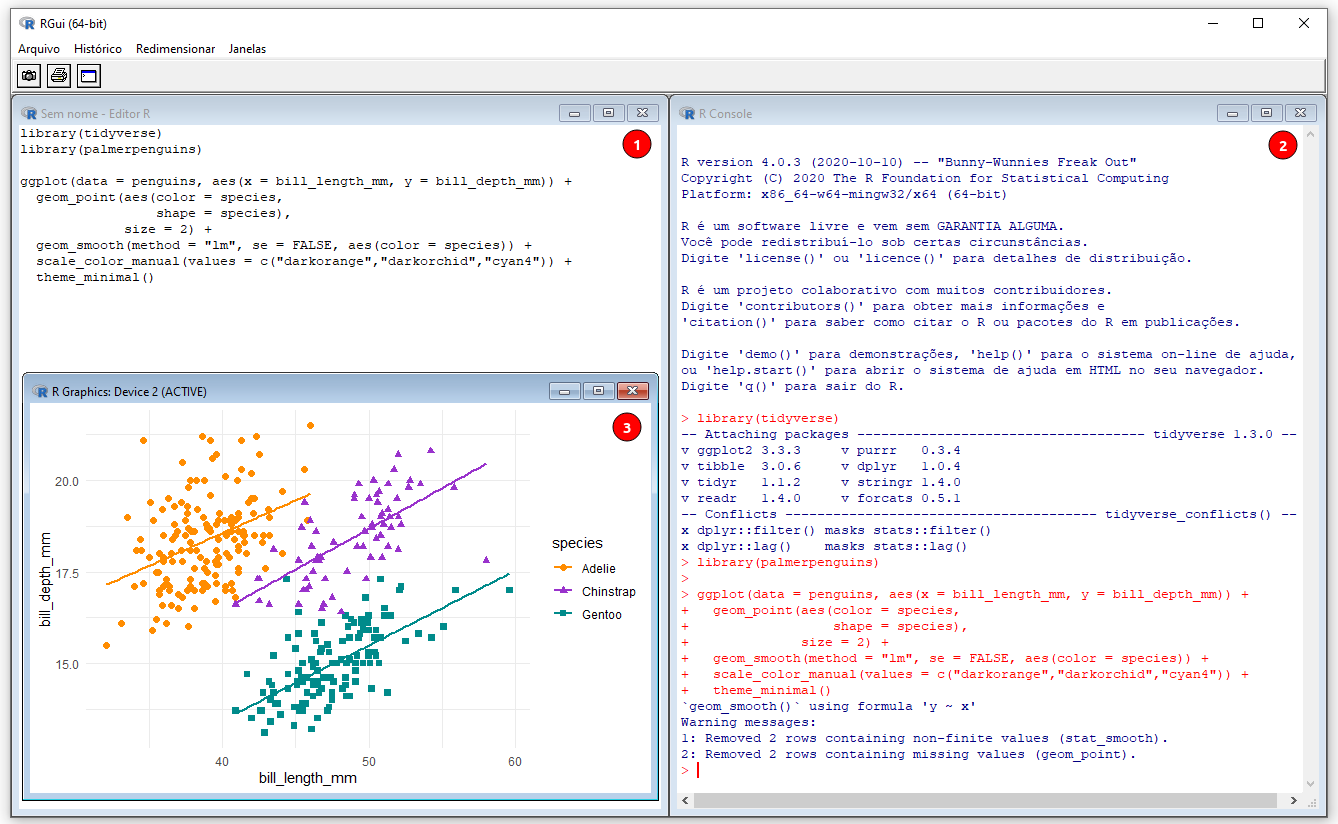
\includegraphics[width=0.7\linewidth]{img/cap04_fig01} 

}

\caption{Interface do RGui. Os números indicam: (1) R Script, (2) R Console, e (3) R Graphics.}\label{fig:fig-rgui}
\end{figure}

Dessa forma, nesse livro todo, nós que escrevemos utilizamos o RStudio e assumimos que você que está lendo fará o mesmo.

O RStudio permite diversas personalizações, grande parte delas contidas em \texttt{Tools\ \textgreater{}\ Global\ options}. Incentivamos as leitoras e leitores a ``fuçar'', com certa dose de cuidado, nas opções para customização. Dentre essas mudanças, destacamos duas:

\begin{enumerate}
\def\labelenumi{\arabic{enumi}.}
\tightlist
\item
  \texttt{Tools\ \textgreater{}\ Global\ options\ \textgreater{}\ Appearance\ \textgreater{}\ Editor\ theme} para escolher um tema para seu RStudio
\item
  \texttt{Tools\ \textgreater{}\ Global\ options\ \textgreater{}\ Code\ \textgreater{}\ {[}X{]}\ Soft-wrap\ R\ source\ files} com essa opção habilitada, quando escrevemos comentários longos ou mudamos a largura da janela que estamos trabalhando, todo o texto e o código se ajustam a janela automaticamente
\end{enumerate}

Um último ponto importante: para evitar possíveis erros é importante instalar primeiro o software que possui a linguagem R e depois o IDE RStudio.

\hypertarget{funcionamento-da-linguagem-r}{%
\section{Funcionamento da linguagem R}\label{funcionamento-da-linguagem-r}}

Nesta seção, veremos os principais conceitos para entender como a linguagem R funciona ou como geralmente utilizamos o IDE RStudio no dia a dia, para executar nossas rotinas utilizando a linguagem R. Veremos então: 1) console, 2) script, 3) operadores, 4) objetos, 5) funções, 6) pacotes, 7) ajuda (\emph{help}), 8) ambiente (\emph{environment/workspace}), 9) citações e 10) principais erros.

Antes de iniciarmos o uso do R pelo RStudio é fundamental entendermos alguns pontos sobre as janelas e o funcionamento delas no RStudio (Figura \ref{fig:fig-rstudio}).

\begin{figure}

{\centering 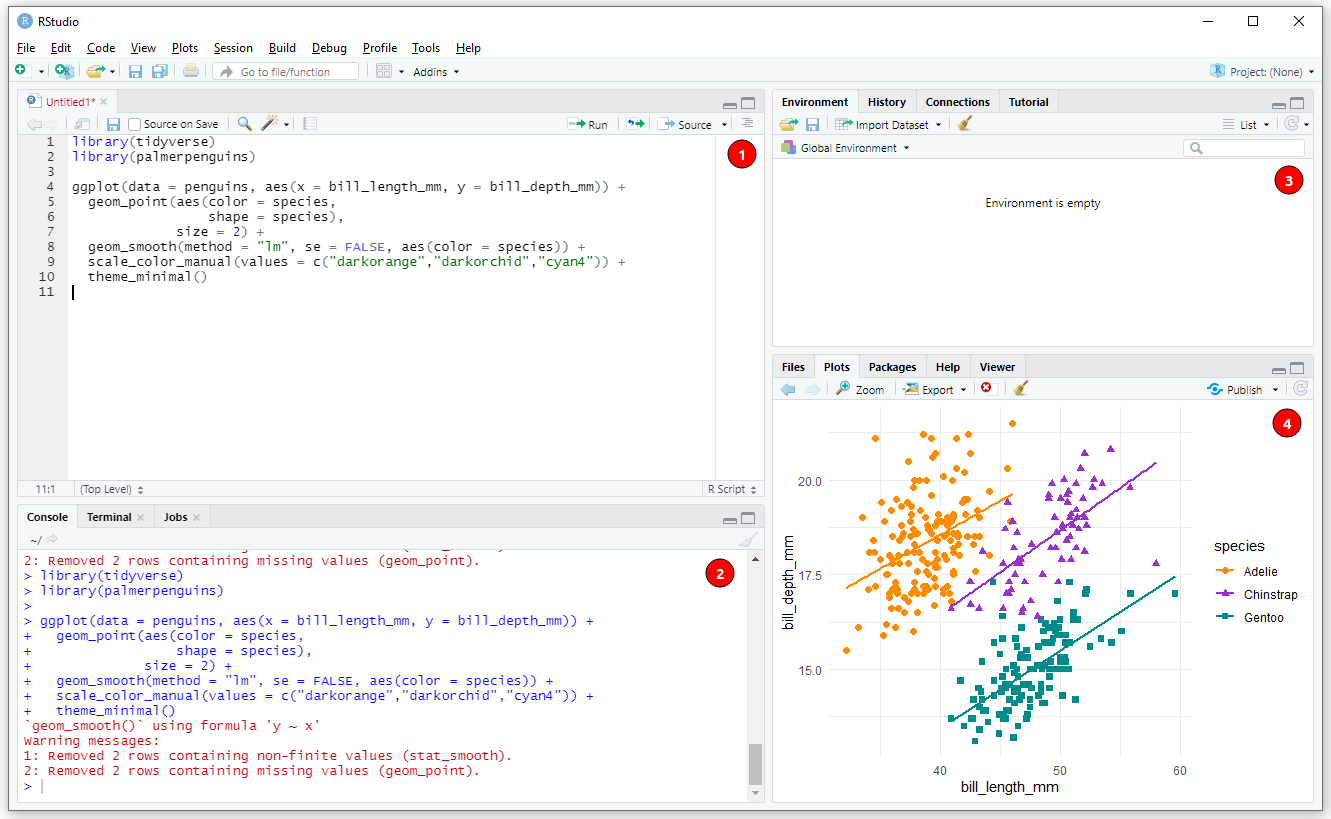
\includegraphics[width=0.7\linewidth]{img/cap04_fig02} 

}

\caption{Interface do RStudio. Os números indicam: (1) janela com abas de Script, R Markdown, dentre outras; (2) janela com abas de Console, Terminal e Jobs; (3) janela com abas de Environment, History, Conections e Tutorial; e (4) janela com abas de Files, Plots, Packages, Help e Viewer.}\label{fig:fig-rstudio}
\end{figure}

Detalhando algumas dessas janelas e abas, temos:

\begin{itemize}
\tightlist
\item
  \textbf{Console}: painel onde os códigos são rodados e vemos as saídas
\item
  \textbf{Editor/Script}: painel onde escrevemos nossos códigos em R, R Markdown ou outro formato
\item
  \textbf{Environment}: painel com todos os objetos criados na sessão
\item
  \textbf{History}: painel com o histórico dos códigos rodados
\item
  \textbf{Files}: painel que mostra os arquivos no diretório de trabalho
\item
  \textbf{Plots}: painel onde os gráficos são apresentados
\item
  \textbf{Packages}: painel que lista os pacotes
\item
  \textbf{Help}: painel onde a documentação das funções é exibida
\end{itemize}

No RStudio, alguns atalhos são fundamentais para aumentar nossa produtividade:

\begin{itemize}
\tightlist
\item
  \textbf{F1}: abre o painel de \emph{Help} quando digitado em cima de uma função
\item
  \textbf{Ctrl + Enter}: roda a linha de código selecionada no script
\item
  \textbf{Ctrl + Shift + N}: abre um novo script
\item
  \textbf{Ctrl + S}: salva um script
\item
  \textbf{Ctrl + Z}: desfaz uma operação
\item
  \textbf{Ctrl + Shift + Z}: refaz uma operação
\item
  \textbf{Alt + -}: insere um sinal de atribuição (\textless-)
\item
  \textbf{Ctrl + Shift + M}: insere um operador pipe (\%\textgreater\%)
\item
  \textbf{Ctrl + Shift + C}: comenta uma linha no script - insere um (\#)
\item
  \textbf{Ctrl + Shift + R}: insere uma sessão (\# ----------------------)
\item
  \textbf{Ctrl + Shift + H}: abre uma janela para selecionar o diretório de trabalho
\item
  \textbf{Ctrl + Shift + F10}: reinicia o console
\item
  \textbf{Ctrl + L}: limpa os códigos do console
\item
  \textbf{Alt + Shift + K}: abre uma janela com todos os atalhos disponíveis
\end{itemize}

\hypertarget{console}{%
\subsection{Console}\label{console}}

O console é onde a versão da linguagem R instalada é carregada para executar os códigos da linguagem R (Figura \ref{fig:fig-rstudio} (2)). Na janela do console aparecerá o símbolo \texttt{\textgreater{}} seguida de uma barra vertical \texttt{\textbar{}} que fica piscando, onde digitaremos ou enviaremos nossos códigos do script. Podemos fazer um pequeno exercício: vamos digitar \texttt{10\ +\ 2}, seguido da tecla \texttt{Enter} para que essa operação seja executada.

\begin{Shaded}
\begin{Highlighting}[]
\DecValTok{10} \SpecialCharTok{+} \DecValTok{2}
\CommentTok{\#\textgreater{} [1] 12}
\end{Highlighting}
\end{Shaded}

O resultado retorna o valor \texttt{12}, precedido de um valor entre colchetes. Esses colchetes demonstram a posição do elemento numa sequência de valores. Se fizermos essa outra operação \texttt{1:42}, o R vai criar uma sequência unitária de valores de 1 a 42. A depender da largura da janela do console, vai aparecer um número diferente entre colchetes indicando sua posição na sequência: antes do 1 vai aparecer o \texttt{{[}1{]}}, depois quando a sequência for quebrada, vai aparecer o número correspondente da posição do elemento, por exemplo, \texttt{{[}26{]}}.

\begin{Shaded}
\begin{Highlighting}[]
\DecValTok{1}\SpecialCharTok{:}\DecValTok{42}
\CommentTok{\#\textgreater{}  [1]  1  2  3  4  5  6  7  8  9 10 11 12 13 14 15 16 17 18 19 20 21 22 23 24 25}
\CommentTok{\#\textgreater{} [26] 26 27 28 29 30 31 32 33 34 35 36 37 38 39 40 41 42}
\end{Highlighting}
\end{Shaded}

Podemos ver o histórico dos códigos executados no Console na aba \textbf{History} (Figura \ref{fig:fig-rstudio} (3)).

\hypertarget{scripts}{%
\subsection{Scripts}\label{scripts}}

Scripts são rascunhos dos códigos e onde de fato os códigos são escritos e depois enviados ao console (Figura \ref{fig:fig-rstudio} (1)). Scripts são arquivos de texto simples, criados com a extensão (terminação) \texttt{.R} (ative a visualização da extensão de arquivos para ver). Para criar um script, basta ir em \texttt{File\ \textgreater{}\ New\ File\ \textgreater{}\ R\ Script}, ou clicando no ícone logo abaixo de \texttt{File}, ou ainda usando o atalho \texttt{Ctrl\ +\ Shift\ +\ N}.

Também é possível usar outro editor de códigos, como o bloco de notas \texttt{.txt}, \href{https://www.sublimetext.com}{Sublime Text}, \href{https://notepad-plus-plus.org}{Notepad++} e similares. Os códigos podem ser escritos nesses editores e depois salvos com a extensão \texttt{.R} que ao ser aberto no RStudio irão ser executados normalmente.

Uma vez escrito os códigos no script podemos rodar esses códigos de duas formas: 1) todo o script de uma vez, clicando em \textbf{Source} ou usando o atalho \texttt{Ctrl\ +\ Shift\ +\ Enter}; ou 2) apenas a linha onde o cursor estiver posicionado, independente de sua posição naquela linha, clicando em \textbf{Run} ou usando o atalho \texttt{Ctrl\ +\ Enter}.

Devemos sempre salvar nossos scripts, tomando por via de regra: primeiro criar o arquivo e depois ir salvando nesse mesmo arquivo a cada passo de desenvolvimento das análises (não é raro o R fechar sozinho e você perder algum tempo de trabalho\ldots). Há diversos motivos para criar um script: continuar o desenvolvimento do mesmo em outro momento ou em outro computador, preservar trabalhos passados, ou ainda compartilhar seus códigos com outra pessoa. Para criar ou salvar um script basta ir em \texttt{File\ \textgreater{}\ Save}, escolher um diretório e nome para o script e salvar. Podemos ainda utilizar o atalho \texttt{Ctrl\ +\ S}.

Em relação aos scripts, ainda há os comentários, representados pelos símbolos \texttt{\#} (hash) ou \texttt{\#\textquotesingle{}} (hash-linha). A diferença entre eles é que para o segundo, quando precionamos a tecla \texttt{Enter} o comentário \texttt{\#\textquotesingle{}} é inserido automaticamente na linha seguinte. Linhas de códigos do script contendo comentários em seu início não são lidos pelo console do R. Se o comentário estiver no final da linha, essa linha de código ainda será lida. Os comentários são utilizados geralmente para: 1) descrever informações sobre dados ou funções e/ou 2) suprimir linhas de código.

É interessante ter no início de cada script um cabeçalho identificando o objetivo ou análise, autor e data para facilitar o compartilhamento e reprodutibilidade. Os comentários podem ser inseridos ou retirados das linhas com o atalho: \texttt{Ctrl\ +\ Shift\ +\ C}.

\begin{Shaded}
\begin{Highlighting}[]
\CommentTok{\#\textquotesingle{} {-}{-}{-}}
\CommentTok{\#\textquotesingle{} Título: Capítulo 04 {-} Introdução ao R}
\CommentTok{\#\textquotesingle{} Autor: Maurício Vancine}
\CommentTok{\#\textquotesingle{} Data: 20{-}05{-}2021}
\CommentTok{\#\textquotesingle{} {-}{-}{-}}
\end{Highlighting}
\end{Shaded}

Além disso, podemos usar comentários para adicionar informações sobre os códigos.

\begin{Shaded}
\begin{Highlighting}[]
\DocumentationTok{\#\# Comentários}
\CommentTok{\# O R nao lê a linha do código depois do \# (hash).}
\DecValTok{42} \CommentTok{\# Essas palavras não são executadas, apenas o 42, a resposta para questão fundamental da vida, o universo e tudo mais.}
\CommentTok{\#\textgreater{} [1] 42}
\end{Highlighting}
\end{Shaded}

Por fim, outro ponto fundamental é ter boas práticas de estilo de código. Quanto mais organizado e padronizado estiver os scripts, mais fácil de entendê-los e de procurar possíveis erros. Existem dois guias de boas práticas para adequar seus scripts: \href{http://adv-r.had.co.nz/Style.html}{Hadley Wickham} e \href{https://google.github.io/styleguide/Rguide.xml}{Google}.

Ainda temos os \emph{Code Snippets} (Fragmentos de código), que são macros de texto usadas para inserir rapidamente fragmentos comuns de código. Por exemplo, o snippet \texttt{fun} insere uma definição de função R. Para mais detalhes, ler o artigo do RStudio: \href{https://support.rstudio.com/hc/en-us/articles/204463668-Code-Snippets}{link}.

\begin{Shaded}
\begin{Highlighting}[]
\CommentTok{\# fun \{snippet\}}
\NormalTok{fun}
\NormalTok{name }\OtherTok{\textless{}{-}} \ControlFlowTok{function}\NormalTok{(variables) \{}
    
\NormalTok{\}}
\end{Highlighting}
\end{Shaded}

Uma aplicação bem interessante dos \emph{Code Snippets} no script é o \texttt{ts}. Basta digitar esse código e em seguida completar um a tecla \texttt{Tab} para inserir rapidamente a data e horário atuais no script em forma de comentário.

\begin{Shaded}
\begin{Highlighting}[]
\CommentTok{\# ts \{snippet\}}
\CommentTok{\# Mon Jul 26 11:25:03 2021 {-}{-}{-}{-}{-}{-}{-}{-}{-}{-}{-}{-}{-}{-}{-}{-}{-}{-}{-}{-}{-}{-}{-}{-}{-}{-}{-}{-}{-}{-}}
\end{Highlighting}
\end{Shaded}

\hypertarget{operadores}{%
\subsection{Operadores}\label{operadores}}

No R, temos cinco tipos de operadores: aritméticos, relacionais, lógicos, atribuição e diversos. Grande parte deles são descritos na Tabela \ref{tab:tab-operadores}.

\begin{table}

\caption{\label{tab:tab-operadores}Operadores no R.}
\centering
\begin{tabular}[t]{c|c|c}
\hline
Operador & Tipo & Descrição\\
\hline
+ & Aritmético & Adição\\
\hline
- & Aritmético & Subtração\\
\hline
* & Aritmético & Multiplicação\\
\hline
/ & Aritmético & Divisão\\
\hline
\%\% & Aritmético & Resto da divisão\\
\hline
\%/\% & Aritmético & Divisão inteira\\
\hline
\textasciicircum{} ou ** & Aritmético & Expoente\\
\hline
> & Relacional & Maior\\
\hline
< & Relacional & Menor\\
\hline
>= & Relacional & Maior ou igual\\
\hline
<= & Relacional & Menor ou igual\\
\hline
== & Relacional & Igualdade\\
\hline
!= & Relacional & Diferença\\
\hline
! & Lógico & Lógico NÃO\\
\hline
\& & Lógico & Lógico elementar E\\
\hline
| & Lógico & Lógico elementar OU\\
\hline
\&\& & Lógico & Lógico E\\
\hline
|| & Lógico & Lógico OU\\
\hline
<- ou = & Atribuição & Atribuição à esquerda\\
\hline
<<- & Atribuição & Super atribuição à esquerda\\
\hline
-> & Atribuição & Atribuição à direita\\
\hline
->> & Atribuição & Super atribuição à direita\\
\hline
: & Diversos & Sequência unitária\\
\hline
\%in\% & Diversos & Elementos que pertencem a um vetor\\
\hline
\%*\% & Diversos & Multiplicar matriz com sua transposta\\
\hline
\%>\% & Diversos & Pipe (pacote magrittr)\\
\hline
|> & Diversos & Pipe (R base nativo)\\
\hline
\%--\% & Diversos & Intervalo de datas (pacote lubridate)\\
\hline
\end{tabular}
\end{table}

Como exemplo, podemos fazer operações simples usando os operadores aritméticos.

\begin{Shaded}
\begin{Highlighting}[]
\DocumentationTok{\#\# Operações aritméticas}
\DecValTok{10} \SpecialCharTok{+} \DecValTok{2} \CommentTok{\# adição}
\CommentTok{\#\textgreater{} [1] 12}
\DecValTok{10} \SpecialCharTok{*} \DecValTok{2} \CommentTok{\# multiplicação}
\CommentTok{\#\textgreater{} [1] 20}
\end{Highlighting}
\end{Shaded}

Precisamos ficar atentos à prioridade dos operadores aritméticos:

\begin{quote}
\textbf{\texttt{PRIORITÁRIO}} \texttt{()} \textgreater{} \texttt{\^{}} \textgreater{} \texttt{*\ ou\ /} \textgreater{} \texttt{+\ ou\ -} \textbf{\texttt{NÃO\ PRIORITÁRIO}}
\end{quote}

Veja no exemplo abaixo como o uso dos parênteses muda o resultado.

\begin{Shaded}
\begin{Highlighting}[]
\DocumentationTok{\#\# Sem especificar a ordem}
\CommentTok{\# Segue a ordem dos operadores.}
\DecValTok{1} \SpecialCharTok{*} \DecValTok{2} \SpecialCharTok{+} \DecValTok{2} \SpecialCharTok{/} \DecValTok{2} \SpecialCharTok{\^{}} \DecValTok{2}
\CommentTok{\#\textgreater{} [1] 2.5}

\DocumentationTok{\#\# Especificando a ordem}
\CommentTok{\# Segue a ordem dos parenteses.}
\NormalTok{((}\DecValTok{1} \SpecialCharTok{*} \DecValTok{2}\NormalTok{) }\SpecialCharTok{+}\NormalTok{ (}\DecValTok{2} \SpecialCharTok{/} \DecValTok{2}\NormalTok{)) }\SpecialCharTok{\^{}} \DecValTok{2}
\CommentTok{\#\textgreater{} [1] 9}
\end{Highlighting}
\end{Shaded}

\hypertarget{objetos}{%
\subsection{Objetos}\label{objetos}}

Objetos são palavras às quais são atribuídos dados. A atribuição possibilita a manipulação de dados ou resultados de análises. Utilizaremos os símbolos \texttt{\textless{}} (menor), seguido de \texttt{-} (menos), sem espaço, dessa forma \texttt{\textless{}-}. Também podemos utilizar o símbolo de igual (\texttt{=}), mas não recomendamos, por não fazer parte das boas práticas de escrita de códigos em R. Podemos inserir essa combinação de símbolos com o atalho \texttt{Alt\ +\ -}. Para demonstrar, vamos atribuir o valor \texttt{10} à palavra \texttt{obj\_10}, e chamar esse objeto novamente para verificar seu conteúdo.

\begin{Shaded}
\begin{Highlighting}[]
\DocumentationTok{\#\# Atribuição {-} símbolo (\textless{}{-})}
\NormalTok{obj\_10 }\OtherTok{\textless{}{-}} \DecValTok{10}
\NormalTok{obj\_10}
\CommentTok{\#\textgreater{} [1] 10}
\end{Highlighting}
\end{Shaded}

Todos os objetos criados numa sessão do R ficam listados na aba \textbf{Environment} (Figura \ref{fig:fig-rstudio} (3)). Além disso, o RStudio possui a função \emph{autocomplete}, ou seja, podemos digitar as primeiras letras de um objeto (ou função) e em seguida apertar \texttt{Tab} para que o RStudio liste tudo que começar com essas letras.

Dois pontos importantes sobre atribuições: primeiro, o R sobrescreve os valores dos objetos com o mesmo nome, deixando o objeto com o valor da segunda atribuição.

\begin{Shaded}
\begin{Highlighting}[]
\DocumentationTok{\#\# Sobrescreve o valor dos objetos}
\NormalTok{obj }\OtherTok{\textless{}{-}} \DecValTok{100}
\NormalTok{obj}
\CommentTok{\#\textgreater{} [1] 100}

\DocumentationTok{\#\# O objeto \textquotesingle{}obj\textquotesingle{} agora vale 2}
\NormalTok{obj }\OtherTok{\textless{}{-}} \DecValTok{2}
\NormalTok{obj}
\CommentTok{\#\textgreater{} [1] 2}
\end{Highlighting}
\end{Shaded}

Segundo, o R tem limitações ao nomear objetos:

\begin{itemize}
\tightlist
\item
  nome de objetos só podem começar por letras (\texttt{a-z} ou \texttt{A-Z}) ou pontos (\texttt{.})
\item
  nome de objetos só podem conter letras (\texttt{a-z} ou \texttt{A-Z}), números (\texttt{0-9}), underscores (\texttt{\_}) ou pontos (\texttt{.})
\item
  R é \emph{case-sensitive}, i.e., ele reconhece letras maiúsculas como diferentes de letras minúscula. Assim, um objeto chamado ``resposta'' é diferente do objeto ``RESPOSTA''
\item
  devemos evitar acentos ou cedilha (\texttt{ç}) para facilitar a memorização dos objetos e também para evitar erros de encoding/codificação de caracteres
\item
  nome de objetos não podem ser iguais a nomes especiais, reservados para programação (\texttt{break}, \texttt{else}, \texttt{FALSE}, \texttt{for}, \texttt{function}, \texttt{if}, \texttt{Inf}, \texttt{NA}, \texttt{NaN}, \texttt{next}, \texttt{repeat}, \texttt{return}, \texttt{TRUE}, \texttt{while})
\end{itemize}

Podemos ainda utilizar objetos para fazer operações e criar objetos. Isso pode parecer um pouco confuso para os iniciantes na linguagem, mas é fundamental aprender essa lógica para passar para os próximos passos.

\begin{Shaded}
\begin{Highlighting}[]
\DocumentationTok{\#\# Definir dois objetos}
\NormalTok{va1 }\OtherTok{\textless{}{-}} \DecValTok{10}
\NormalTok{va2 }\OtherTok{\textless{}{-}} \DecValTok{2}

\DocumentationTok{\#\# Operações com objetos e atribuicão}
\NormalTok{adi }\OtherTok{\textless{}{-}}\NormalTok{ va1 }\SpecialCharTok{+}\NormalTok{ va2}
\NormalTok{adi}
\CommentTok{\#\textgreater{} [1] 12}
\end{Highlighting}
\end{Shaded}

\hypertarget{funuxe7uxf5es}{%
\subsection{Funções}\label{funuxe7uxf5es}}

Funções são códigos preparados para realizar uma tarefa específica de modo simples. Outra forma de entender uma função é: códigos que realizam operações em argumentos. A estrutura de uma função é muito similar à sintaxe usada em planilhas eletrônicas, sendo composta por:

\begin{quote}
nome\_da\_função(argumento1, argumento2, \ldots)
\end{quote}

\begin{enumerate}
\def\labelenumi{\arabic{enumi}.}
\tightlist
\item
  \textbf{Nome da função}: remete ao que ela faz
\item
  \textbf{Parênteses}: limitam a função
\item
  \textbf{Argumentos}: valores, parâmetros ou expressões onde a função atuará
\item
  \textbf{Vírgulas}: separam os argumentos
\end{enumerate}

Os argumentos de uma função podem ser de dois tipos:

\begin{enumerate}
\def\labelenumi{\arabic{enumi}.}
\tightlist
\item
  \textbf{Valores ou objetos}: a função alterará os valores em si ou os valores atribuídos aos objetos
\item
  \textbf{Parâmetros}: valores fixos que informam um método ou a realização de uma operação. Informa-se o nome desse argumento, seguido de ``='' e um número, texto ou TRUE ou FALSE
\end{enumerate}

Alguns exemplos de argumentos como valores ou objetos.

\begin{Shaded}
\begin{Highlighting}[]
\DocumentationTok{\#\# Funções {-} argumentos como valores}
\FunctionTok{sum}\NormalTok{(}\DecValTok{10}\NormalTok{, }\DecValTok{2}\NormalTok{)}
\CommentTok{\#\textgreater{} [1] 12}

\DocumentationTok{\#\# Funções {-} argumentos como objetos}
\FunctionTok{sum}\NormalTok{(va1, va2)}
\CommentTok{\#\textgreater{} [1] 12}
\end{Highlighting}
\end{Shaded}

Alguns exemplos de argumentos como parâmetros. Note que apesar do valor do argumento ser o mesmo (10), seu efeito no resultado muda drasticamente. Aqui também é importante destacar um ponto: 1) podemos informar os argumentos sequencialmente, sem explicitar seus nomes, ou 2) independente da ordem, mas explicitando seus nomes. Entretanto, como no exemplo abaixo, devemos informar o nome do argumento (i.e., parâmetro), para que seu efeito seja o que desejamos.

\begin{Shaded}
\begin{Highlighting}[]
\DocumentationTok{\#\# Funções {-} argumentos como parâmetros}
\DocumentationTok{\#\# Repetição {-} repete todos os elementos}
\FunctionTok{rep}\NormalTok{(}\AttributeTok{x =} \DecValTok{1}\SpecialCharTok{:}\DecValTok{5}\NormalTok{, }\AttributeTok{times =} \DecValTok{10}\NormalTok{)}
\CommentTok{\#\textgreater{}  [1] 1 2 3 4 5 1 2 3 4 5 1 2 3 4 5 1 2 3 4 5 1 2 3 4 5 1 2 3 4 5 1 2 3 4 5 1 2 3}
\CommentTok{\#\textgreater{} [39] 4 5 1 2 3 4 5 1 2 3 4 5}

\DocumentationTok{\#\# Repetição {-} repete cada um dos elementos}
\FunctionTok{rep}\NormalTok{(}\AttributeTok{x =} \DecValTok{1}\SpecialCharTok{:}\DecValTok{5}\NormalTok{, }\AttributeTok{each =} \DecValTok{10}\NormalTok{)}
\CommentTok{\#\textgreater{}  [1] 1 1 1 1 1 1 1 1 1 1 2 2 2 2 2 2 2 2 2 2 3 3 3 3 3 3 3 3 3 3 4 4 4 4 4 4 4 4}
\CommentTok{\#\textgreater{} [39] 4 4 5 5 5 5 5 5 5 5 5 5}
\end{Highlighting}
\end{Shaded}

Um ponto fundamental, e que deve ser entendido nesse ponto, é o fluxo de atribuições do resultado da operação de funções a novos objetos. No desenvolvimento de qualquer script na linguagem R, grande parte da estrutura do mesmo será dessa forma: atribuição de dados \textgreater{} operações com funções \textgreater{} atribuição dos resultados a novos objetos \textgreater{} operações com funções desses novos objetos \textgreater{} atribuição dos resultados a novos objetos\ldots{} Ao entender esse funcionamento, começamos a entender como devemos pensar na organização do nosso script para montar as análises que precisamos.

\begin{Shaded}
\begin{Highlighting}[]
\DocumentationTok{\#\# Atribuicão dos resultados}
\DocumentationTok{\#\# Repetição}
\NormalTok{rep\_times }\OtherTok{\textless{}{-}} \FunctionTok{rep}\NormalTok{(}\DecValTok{1}\SpecialCharTok{:}\DecValTok{5}\NormalTok{, }\AttributeTok{times =} \DecValTok{10}\NormalTok{)}
\NormalTok{rep\_times}
\CommentTok{\#\textgreater{}  [1] 1 2 3 4 5 1 2 3 4 5 1 2 3 4 5 1 2 3 4 5 1 2 3 4 5 1 2 3 4 5 1 2 3 4 5 1 2 3}
\CommentTok{\#\textgreater{} [39] 4 5 1 2 3 4 5 1 2 3 4 5}

\DocumentationTok{\#\# Somar e atribuir}
\NormalTok{rep\_times\_soma }\OtherTok{\textless{}{-}} \FunctionTok{sum}\NormalTok{(rep\_times)}
\NormalTok{rep\_times\_soma}
\CommentTok{\#\textgreater{} [1] 150}

\DocumentationTok{\#\# Raiz e atribuir}
\NormalTok{rep\_times\_soma\_raiz }\OtherTok{\textless{}{-}} \FunctionTok{sqrt}\NormalTok{(rep\_times\_soma)}
\NormalTok{rep\_times\_soma\_raiz}
\CommentTok{\#\textgreater{} [1] 12.24745}
\end{Highlighting}
\end{Shaded}

Por fim, é fundamental também entender a origem das funções que usamos no R. Todas as funções são advindas de pacotes. Esses pacotes possuem duas origens.

\begin{enumerate}
\def\labelenumi{\arabic{enumi}.}
\tightlist
\item
  pacotes já instalados por padrão e que são carregados quando abrimos o R (\emph{R Base})
\item
  pacotes que instalamos e carregamos com funções
\end{enumerate}

\hypertarget{pacotes-1}{%
\subsection{Pacotes}\label{pacotes-1}}

Pacotes são conjuntos extras de funções para executar tarefas específicas, além do \emph{R Base}. Existe literalmente milhares de pacotes para as mais diversas tarefas: estatística, ecologia, geografia, sensoriamento remoto, econometria, ciências sociais, gráficos, \emph{machine learning}, etc. Podemos verificar este vasto conjunto de pacotes pelo \href{https://cran.r-project.org/web/packages/available_packages_by_name.html}{link} que lista por nome os pacotes oficiais, ou seja, que passaram pelo crivo do \textbf{CRAN}. Existem ainda muito mais pacotes em desenvolvimento, geralmente disponibilizados em repositórios do \textbf{GitHub} ou \textbf{GitLab}.

Primeiramente, com uma sessão do R sem carregar nenhum pacote extra, podemos verificar pacotes carregados pelo \emph{R Base} utilizando a função \texttt{search()}.

\begin{Shaded}
\begin{Highlighting}[]
\DocumentationTok{\#\# Verificar pacotes carregados}
\FunctionTok{search}\NormalTok{()}
\end{Highlighting}
\end{Shaded}

Podemos ainda verificar todos pacotes instalados em seu computador com a função \texttt{library()}.

\begin{Shaded}
\begin{Highlighting}[]
\DocumentationTok{\#\# Verificar pacotes instalados}
\FunctionTok{library}\NormalTok{()}
\end{Highlighting}
\end{Shaded}

No R, quando tratamos de pacotes, devemos destacar a diferença de dois conceitos: instalar um pacote e carregar um pacote. A instalação de pacotes possui algumas características:

\begin{itemize}
\tightlist
\item
  Instala-se um pacote apenas uma vez
\item
  Precisamos estar conectados à internet
\item
  O nome do pacote precisa estar entre aspas na função
\item
  Função (CRAN): \texttt{install.packages()}
\end{itemize}

Vamos instalar o pacote \texttt{vegan} diretamente do CRAN, que possui funções para realizar uma série de análise em ecologia. Para isso, podemos ir em \texttt{Tools\ \textgreater{}\ Install\ Packages...}, ou ir na aba \textbf{Packages} (Figura \ref{fig:fig-rstudio} (4)), procurar o pacote e simplesmente clicar em ``Install''. Podemos ainda utilizar a função \texttt{install.packages()}.

\begin{Shaded}
\begin{Highlighting}[]
\DocumentationTok{\#\# Instalar pacotes}
\FunctionTok{install.packages}\NormalTok{(}\StringTok{"vegan"}\NormalTok{)}
\end{Highlighting}
\end{Shaded}

Podemos conferir em que diretórios um pacote será instalado com a função \texttt{.libPaths()}.

\begin{Shaded}
\begin{Highlighting}[]
\DocumentationTok{\#\# Diretórios de intalação dos pacotes}
\FunctionTok{.libPaths}\NormalTok{()}
\CommentTok{\#\textgreater{} [1] "C:/Users/pater/Documents/R/win{-}library/4.0"}
\CommentTok{\#\textgreater{} [2] "C:/Program Files/R/R{-}4.0.5/library"}
\end{Highlighting}
\end{Shaded}

Uma vez instalado um pacote, não há necessidade de instalá-lo novamente. Entretanto, todas as vezes que iniciarmos uma sessão no R, precisamos carregar os pacotes com as funções que precisamos utilizar. O carregamento de pacotes possui algumas características:

\begin{itemize}
\tightlist
\item
  Carrega-se o pacote toda vez que se abre uma nova sessão do R
\item
  Não precisamos estar conectados à internet
\item
  O nome do pacote não precisa estar entre aspas na função
\item
  Funções: \texttt{library()} ou \texttt{require()}
\end{itemize}

Vamos carregar o pacote \texttt{vegan} que instalamos anteriormente. Podemos ir na aba \textbf{Packages} (Figura \ref{fig:fig-rstudio} (4)) e ``ticar'' o pacote que queremos carregar ou utilizar a função \texttt{library()}.

\begin{Shaded}
\begin{Highlighting}[]
\DocumentationTok{\#\# Carregar pacotes}
\FunctionTok{library}\NormalTok{(vegan)}
\end{Highlighting}
\end{Shaded}

Como dissemos, alguns pacotes em desenvolvimento encontram-se disponíveis em repositórios do GitHub ou GitLab. Para instalar pacotes do GitHub, por exemplo, precisamos instalar e carregar o pacote \texttt{devtools}.

\begin{Shaded}
\begin{Highlighting}[]
\DocumentationTok{\#\# Instalar pacote devtools}
\FunctionTok{install.packages}\NormalTok{(}\StringTok{"devtools"}\NormalTok{)}

\DocumentationTok{\#\# Carregar pacote devtools}
\FunctionTok{library}\NormalTok{(devtools)}
\end{Highlighting}
\end{Shaded}

Uma vez instalado e carregado esse pacote, podemos instalar o pacote do GitHub, utilizando a função \texttt{devtools::install\_github()}. Precisamos atentar para usar essa forma ``nome\_usuario/nome\_repositorio'', retirados do link do repositório de interesse. Como exemplo, podemos instalar o mesmo pacote \texttt{vegan} do repositório do GitHub \href{https://github.com/vegandevs/vegan}{vegandevs/vegan}, e depois utilizar a função \texttt{library()} para carregá-lo normalmente.

\begin{Shaded}
\begin{Highlighting}[]
\DocumentationTok{\#\# Instalar pacote do github}
\NormalTok{devtools}\SpecialCharTok{::}\FunctionTok{install\_github}\NormalTok{(}\StringTok{"vegandevs/vegan"}\NormalTok{)}

\DocumentationTok{\#\# Carregar pacote do github}
\FunctionTok{library}\NormalTok{(}\StringTok{"vegan"}\NormalTok{)}
\end{Highlighting}
\end{Shaded}

Pode ser que em algumas circunstâncias iremos precisar instalar pacotes com versões específicas para algumas análises. A forma mais simples de fazer isso é instalar um pacote a partir de um arquivo compactado \texttt{.tar.gz}. Para isso podemos ir à base do CRAN e realizar o download: \url{https://cran.r-project.org/src/contrib/Archive/}. Para exemplificar, vamos instalar o pacote \texttt{vegan\ 2.4.0}.

\begin{Shaded}
\begin{Highlighting}[]
\DocumentationTok{\#\# Download do arquivo .tar.gz}
\FunctionTok{download.file}\NormalTok{(}\AttributeTok{url =} \StringTok{"https://cran.r{-}project.org/src/contrib/Archive/vegan/vegan\_2.4{-}0.tar.gz"}\NormalTok{,}
              \AttributeTok{destfile =} \StringTok{"vegan\_2.4{-}0.tar.gz"}\NormalTok{, }\AttributeTok{mode =} \StringTok{"wb"}\NormalTok{)}

\DocumentationTok{\#\# Instalar o pacote vegan 2.4.0}
\FunctionTok{install.packages}\NormalTok{(}\StringTok{"vegan\_2.4{-}0.tar.gz"}\NormalTok{, }\AttributeTok{repos =} \ConstantTok{NULL}\NormalTok{, }\AttributeTok{type =} \StringTok{"source"}\NormalTok{)}
\end{Highlighting}
\end{Shaded}

A maioria dos pacotes vem com bancos de dados que podem ser acessados pela função \texttt{data()}. Esses bancos de dados podem ser usados para testar as funções do pacote. Se estiver com dúvida na maneira como você deve preparar a planilha para realizar uma análise específica, entre no help da função e veja os conjuntos de dados que estão no exemplo desta função. Como exemplo, vamos carregar os dados \texttt{dune} do pacote \texttt{vegan}.

\begin{Shaded}
\begin{Highlighting}[]
\DocumentationTok{\#\# Carregar dados de um pacote}
\FunctionTok{library}\NormalTok{(vegan)}
\FunctionTok{data}\NormalTok{(dune)}
\NormalTok{dune[}\DecValTok{1}\SpecialCharTok{:}\DecValTok{6}\NormalTok{, }\DecValTok{1}\SpecialCharTok{:}\DecValTok{6}\NormalTok{]}
\CommentTok{\#\textgreater{}   Achimill Agrostol Airaprae Alopgeni Anthodor Bellpere}
\CommentTok{\#\textgreater{} 1        1        0        0        0        0        0}
\CommentTok{\#\textgreater{} 2        3        0        0        2        0        3}
\CommentTok{\#\textgreater{} 3        0        4        0        7        0        2}
\CommentTok{\#\textgreater{} 4        0        8        0        2        0        2}
\CommentTok{\#\textgreater{} 5        2        0        0        0        4        2}
\CommentTok{\#\textgreater{} 6        2        0        0        0        3        0}
\end{Highlighting}
\end{Shaded}

Se por algum motivo precisarmos desinstalar um pacote, podemos utilizar a função \texttt{remove.packages()}. Já para descarregar um pacote de uma sessão do R, podemos usar a função \texttt{detach()}.

\begin{Shaded}
\begin{Highlighting}[]
\DocumentationTok{\#\# Descarregar um pacote}
\FunctionTok{detach}\NormalTok{(}\StringTok{"package:vegan"}\NormalTok{, }\AttributeTok{unload =} \ConstantTok{TRUE}\NormalTok{)}
\end{Highlighting}
\end{Shaded}

E um último ponto fundamental sobre pacotes, diz respeito à atualização dos mesmos. Os pacotes são atualizados com frequência, e infelizmente ou felizmente (pois as atualizações podem oferecer algumas quebras entre pacotes), não se atualizam sozinhos. Muitas vezes, a instalação de um pacote pode depender da versão dos pacotes dependentes, e geralmente uma janela se abre perguntando se você quer que todos os pacotes dependentes sejam atualizados. Podemos ir na aba \textbf{Packages} (Figura \ref{fig:fig-rstudio} (4)) e clicar em ``Update'' ou usar a função \texttt{update.packages(checkBuilt\ =\ TRUE,\ ask\ =\ FALSE)} para atualizá-los, entretanto, essa é uma função que costuma demorar muito para terminar de ser executada.

\begin{Shaded}
\begin{Highlighting}[]
\DocumentationTok{\#\# Atualização dos pacotes}
\FunctionTok{update.packages}\NormalTok{(}\AttributeTok{checkBuilt =} \ConstantTok{TRUE}\NormalTok{, }\AttributeTok{ask =} \ConstantTok{FALSE}\NormalTok{)}
\end{Highlighting}
\end{Shaded}

Para fazer a atualização dos pacotes instalados pelo GitHub, recomendamos o uso do pacote \href{https://github.com/hrbrmstr/dtupdate}{\texttt{dtupdate}}.

\begin{Shaded}
\begin{Highlighting}[]
\DocumentationTok{\#\# Atualização dos pacotes instalados pelo GitHub}
\NormalTok{dtupdate}\SpecialCharTok{::}\FunctionTok{github\_update}\NormalTok{(}\AttributeTok{auto.install =} \ConstantTok{TRUE}\NormalTok{, }\AttributeTok{ask =} \ConstantTok{FALSE}\NormalTok{)}
\end{Highlighting}
\end{Shaded}

Destacamos e incentivamos ainda uma prática que achamos interessante para aumentar a reprodutibilidade de nossos códigos e scripts: a de chamar as funções de pacotes carregados dessa forma \texttt{pacote::função()}. Dessa forma, deixamos claro o pacote em que a função está implementada. Destacamos aqui o exemplo de como instalar pacotes do GitHub do pacote \texttt{devtools}.

\begin{Shaded}
\begin{Highlighting}[]
\DocumentationTok{\#\# Pacote seguido da função implementada daquele pacote}
\NormalTok{devtools}\SpecialCharTok{::}\FunctionTok{install\_github}\NormalTok{()}
\end{Highlighting}
\end{Shaded}

\hypertarget{ajuda-help}{%
\subsection{\texorpdfstring{Ajuda (\emph{Help})}{Ajuda (Help)}}\label{ajuda-help}}

Um importante passo para melhorar a usabilidade e ter mais familiaridade com a linguagem R é aprender a usar a ajuda de cada função. Para tanto, podemos utilizar a função \texttt{help()} ou o operador \texttt{?}, depois de ter carregado o pacote, para abrir uma nova aba (Figura \ref{fig:fig-rstudio} (4)) que possui diversas informações sobre a função de interesse. O arquivo de ajuda do R possui geralmente nove ou dez tópicos, que nos auxiliam muito no entendimento dos dados de entrada, argumentos e que operações estão sendo realizadas.

\begin{itemize}
\tightlist
\item
  \textbf{Description}: resumo da função
\item
  \textbf{Usage}: como utilizar a função e quais os seus argumentos
\item
  \textbf{Arguments}: detalha os argumentos e como os mesmos devem ser especificados
\item
  \textbf{Details}: detalhes importantes para se usar a função
\item
  \textbf{Value}: mostra como interpretar a saída (\emph{output}) da função (os resultados)
\item
  \textbf{Note}: notas gerais sobre a função
\item
  \textbf{Authors}: autores da função
\item
  \textbf{References}: referências bibliográficas para os métodos usados para construção da função
\item
  \textbf{See also}: funções relacionadas
\item
  \textbf{Examples}: exemplos do uso da função. Às vezes pode ser útil copiar esse trecho e colar no R para ver como funciona e como usar a função.
\end{itemize}

Vamos realizar um exemplo, buscando o \texttt{help} da função \texttt{aov()}, que realiza uma análise de variância.

\begin{Shaded}
\begin{Highlighting}[]
\DocumentationTok{\#\# Ajuda}
\FunctionTok{help}\NormalTok{(aov)}
\NormalTok{?aov}
\end{Highlighting}
\end{Shaded}

Além das funções, podemos buscar detalhes de um pacote em específico, para uma página simples do \texttt{help} utilizando a função \texttt{help()} ou o operador \texttt{?}. Entretanto, para uma opção que ofereça uma descrição detalhada e um índice de todas as funções do pacote, podemos utilizar a função \texttt{library()}, mas agora utilizando o argumento \texttt{help}, indicando o pacote de interesse entre aspas.

\begin{Shaded}
\begin{Highlighting}[]
\DocumentationTok{\#\# Ajuda do pacote}
\FunctionTok{help}\NormalTok{(vegan)}
\NormalTok{?vegan}

\DocumentationTok{\#\# Help detalhado}
\FunctionTok{library}\NormalTok{(}\AttributeTok{help =} \StringTok{"vegan"}\NormalTok{)}
\end{Highlighting}
\end{Shaded}

Outra ferramenta de busca é a página \href{http://www.rseek.org}{rseek}, na qual é possível buscar por um termo não só nos pacotes do R, mas também em listas de emails, manuais, páginas na internet e livros sobre o programa.

\hypertarget{ambiente-environment}{%
\subsection{\texorpdfstring{Ambiente (\emph{Environment})}{Ambiente (Environment)}}\label{ambiente-environment}}

O ambiente \emph{Environment} como vimos é onde os objetos criados são armazenados. É fundamental entender que um objeto é uma alocação de um pequeno espaço na memória RAM do seu computador, onde o R armazenará um valor ou o resultado de uma função, utilizando o nome que definimos na atribuição. Sendo assim, se fizermos uma atribuição de um objeto maior que o tamanho da memória RAM, esse objeto não será alocado, e a atribuição não funcionará. Existem opções para contornar esse tipo de limitação, mas não a abordaremos aqui. Entretanto, podemos utilizar a função \texttt{object.size()} para saber quanto espaço nosso objeto criado está alocando de memória RAM.

\begin{Shaded}
\begin{Highlighting}[]
\DocumentationTok{\#\# Tamanho de um objeto}
\FunctionTok{object.size}\NormalTok{(adi)}
\CommentTok{\#\textgreater{} 56 bytes}
\end{Highlighting}
\end{Shaded}

Podemos listar todos os objetos criados com a função \texttt{ls()} ou \texttt{objects()}.

\begin{Shaded}
\begin{Highlighting}[]
\DocumentationTok{\#\# Listar todos os objetos}
\FunctionTok{ls}\NormalTok{()}
\CommentTok{\#\textgreater{} [1] "adi"                 "dune"                "obj"                }
\CommentTok{\#\textgreater{} [4] "obj\_10"              "rep\_times"           "rep\_times\_soma"     }
\CommentTok{\#\textgreater{} [7] "rep\_times\_soma\_raiz" "va1"                 "va2"}
\end{Highlighting}
\end{Shaded}

Podemos ainda remover objetos criados com a função \texttt{rm()} ou \texttt{remove()}. Ou ainda fazer uma função composta para remover todos os objetos do \emph{Environment}.

\begin{Shaded}
\begin{Highlighting}[]
\DocumentationTok{\#\# Remover um objeto}
\FunctionTok{rm}\NormalTok{(adi)}

\DocumentationTok{\#\# Remover todos os objetos criados}
\FunctionTok{rm}\NormalTok{(}\AttributeTok{list =} \FunctionTok{ls}\NormalTok{())}
\end{Highlighting}
\end{Shaded}

Quando usamos a função \texttt{ls()} agora, nenhum objeto é listado.

\begin{Shaded}
\begin{Highlighting}[]
\DocumentationTok{\#\# Listar todos os objetos}
\FunctionTok{ls}\NormalTok{()}
\CommentTok{\#\textgreater{} character(0)}
\end{Highlighting}
\end{Shaded}

Toda a vez que fechamos o R os objetos criados são apagados do \textbf{Environment}. Dessa forma, em algumas ocasiões, por exemplo, análises estatísticas que demoram um grande tempo para serem realizadas, pode ser interessante exportar alguns ou todos os objetos criados.

Para salvar todos os objetos, ou seja, todo o \emph{workspace}, podemos ir em \texttt{Session\ -\textgreater{}\ Save\ Workspace\ As...} e escolher o nome do arquivo do \emph{workspace}, por exemplo, ``meu\_workspace.RData''. Podemos ainda utilizar funções para essas tarefas. A função \texttt{save.image()} salva todo \emph{workspace} com a extensão \texttt{.RData}.

\begin{Shaded}
\begin{Highlighting}[]
\DocumentationTok{\#\# Salvar todo o workspace}
\FunctionTok{save.image}\NormalTok{(}\AttributeTok{file =} \StringTok{"meu\_workspace.RData"}\NormalTok{)}
\end{Highlighting}
\end{Shaded}

Depois disso, podemos fechar o RStudio tranquilamente, e quando formos trabalhar novamente, podemos carregar os objetos criados indo em \texttt{Session\ -\textgreater{}\ Load\ Workspace...} ou utilizando a função \texttt{load()}.

\begin{Shaded}
\begin{Highlighting}[]
\DocumentationTok{\#\# Carregar todo o workspace}
\FunctionTok{load}\NormalTok{(}\StringTok{"meu\_workspace.RData"}\NormalTok{)}
\end{Highlighting}
\end{Shaded}

Entretanto, em algumas ocasiões, não precisamos salvar todos os objetos. Dessa forma, podemos salvar apenas alguns objetos específicos usando a função \texttt{save()}, também com a extensão \texttt{.RData}.

\begin{Shaded}
\begin{Highlighting}[]
\DocumentationTok{\#\# Salvar apenas um objeto}
\FunctionTok{save}\NormalTok{(obj1, }\AttributeTok{file =} \StringTok{"meu\_obj.RData"}\NormalTok{)}

\DocumentationTok{\#\# Salvar apenas um objeto}
\FunctionTok{save}\NormalTok{(obj1, obj2, }\AttributeTok{file =} \StringTok{"meus\_objs.RData"}\NormalTok{)}

\DocumentationTok{\#\# Carregar os objetos}
\FunctionTok{load}\NormalTok{(}\StringTok{"meus\_objs.RData"}\NormalTok{)}
\end{Highlighting}
\end{Shaded}

Ou ainda podemos salvar apenas um objeto com a extensão \texttt{.rds}. Para isso, usamos as funções \texttt{saveRDS()} e \texttt{readRDS()}, para exportar e importar esses dados, respectivamente.

\begin{Shaded}
\begin{Highlighting}[]
\DocumentationTok{\#\# Salvar um objeto para um arquivo}
\FunctionTok{saveRDS}\NormalTok{(obj, }\AttributeTok{file =} \StringTok{"meu\_obj.rds"}\NormalTok{)}

\DocumentationTok{\#\# Carregar esse objeto}
\FunctionTok{readRDS}\NormalTok{(}\AttributeTok{file =} \StringTok{"meu\_obj.rds"}\NormalTok{)}
\end{Highlighting}
\end{Shaded}

\hypertarget{citauxe7uxf5es}{%
\subsection{Citações}\label{citauxe7uxf5es}}

Ao utilizar o R para realizar alguma análise em nossos estudos, é fundamental a citação do mesmo. Para saber como citar exatamente o R em artigos, existe uma função denominada \texttt{citation()}, que provê um formato genérico de citação e um BibTeX para arquivos LaTeX e R Markdown.

\begin{Shaded}
\begin{Highlighting}[]
\DocumentationTok{\#\# Citação do R}
\FunctionTok{citation}\NormalTok{()}
\CommentTok{\#\textgreater{} }
\CommentTok{\#\textgreater{} To cite R in publications use:}
\CommentTok{\#\textgreater{} }
\CommentTok{\#\textgreater{}   R Core Team (2021). R: A language and environment for statistical}
\CommentTok{\#\textgreater{}   computing. R Foundation for Statistical Computing, Vienna, Austria.}
\CommentTok{\#\textgreater{}   URL https://www.R{-}project.org/.}
\CommentTok{\#\textgreater{} }
\CommentTok{\#\textgreater{} A BibTeX entry for LaTeX users is}
\CommentTok{\#\textgreater{} }
\CommentTok{\#\textgreater{}   @Manual\{,}
\CommentTok{\#\textgreater{}     title = \{R: A Language and Environment for Statistical Computing\},}
\CommentTok{\#\textgreater{}     author = \{\{R Core Team\}\},}
\CommentTok{\#\textgreater{}     organization = \{R Foundation for Statistical Computing\},}
\CommentTok{\#\textgreater{}     address = \{Vienna, Austria\},}
\CommentTok{\#\textgreater{}     year = \{2021\},}
\CommentTok{\#\textgreater{}     url = \{https://www.R{-}project.org/\},}
\CommentTok{\#\textgreater{}   \}}
\CommentTok{\#\textgreater{} }
\CommentTok{\#\textgreater{} We have invested a lot of time and effort in creating R, please cite it}
\CommentTok{\#\textgreater{} when using it for data analysis. See also \textquotesingle{}citation("pkgname")\textquotesingle{} for}
\CommentTok{\#\textgreater{} citing R packages.}
\end{Highlighting}
\end{Shaded}

No resultado dessa função, há uma mensagem muito interessante: ``See also `citation(``pkgname'')' for citing R packages.''. Dessa forma, aconselhamos os usuários de R a citar também os pacotes que utilizaram em suas análises para dar os devidos créditos aos desenvolvedores das funções implementadas nos pacotes. Como exemplo, vamos ver como fica a citação do pacote \texttt{vegan}.

\begin{Shaded}
\begin{Highlighting}[]
\DocumentationTok{\#\# Citação do pacote vegan}
\FunctionTok{citation}\NormalTok{(}\StringTok{"vegan"}\NormalTok{)}
\CommentTok{\#\textgreater{} }
\CommentTok{\#\textgreater{} To cite package \textquotesingle{}vegan\textquotesingle{} in publications use:}
\CommentTok{\#\textgreater{} }
\CommentTok{\#\textgreater{}   Jari Oksanen, F. Guillaume Blanchet, Michael Friendly, Roeland Kindt,}
\CommentTok{\#\textgreater{}   Pierre Legendre, Dan McGlinn, Peter R. Minchin, R. B. O\textquotesingle{}Hara, Gavin}
\CommentTok{\#\textgreater{}   L. Simpson, Peter Solymos, M. Henry H. Stevens, Eduard Szoecs and}
\CommentTok{\#\textgreater{}   Helene Wagner (2020). vegan: Community Ecology Package. R package}
\CommentTok{\#\textgreater{}   version 2.5{-}7. https://CRAN.R{-}project.org/package=vegan}
\CommentTok{\#\textgreater{} }
\CommentTok{\#\textgreater{} A BibTeX entry for LaTeX users is}
\CommentTok{\#\textgreater{} }
\CommentTok{\#\textgreater{}   @Manual\{,}
\CommentTok{\#\textgreater{}     title = \{vegan: Community Ecology Package\},}
\CommentTok{\#\textgreater{}     author = \{Jari Oksanen and F. Guillaume Blanchet and Michael Friendly and Roeland Kindt and Pierre Legendre and Dan McGlinn and Peter R. Minchin and R. B. O\textquotesingle{}Hara and Gavin L. Simpson and Peter Solymos and M. Henry H. Stevens and Eduard Szoecs and Helene Wagner\},}
\CommentTok{\#\textgreater{}     year = \{2020\},}
\CommentTok{\#\textgreater{}     note = \{R package version 2.5{-}7\},}
\CommentTok{\#\textgreater{}     url = \{https://CRAN.R{-}project.org/package=vegan\},}
\CommentTok{\#\textgreater{}   \}}
\CommentTok{\#\textgreater{} }
\CommentTok{\#\textgreater{} }\AlertTok{ATTENTION}\CommentTok{: This citation information has been auto{-}generated from the}
\CommentTok{\#\textgreater{} package DESCRIPTION file and may need manual editing, see}
\CommentTok{\#\textgreater{} \textquotesingle{}help("citation")\textquotesingle{}.}
\end{Highlighting}
\end{Shaded}

Podemos ainda utilizar a função \texttt{write\_bib()} do pacote \texttt{knitr} para exportar a citação do pacote no formato \texttt{.bib}.

\begin{Shaded}
\begin{Highlighting}[]
\DocumentationTok{\#\# Exportar uma citação em formato .bib}
\NormalTok{knitr}\SpecialCharTok{::}\FunctionTok{write\_bib}\NormalTok{(}\StringTok{"vegan"}\NormalTok{, }\AttributeTok{file =} \StringTok{"vegan\_ex.bib"}\NormalTok{)}
\end{Highlighting}
\end{Shaded}

\hypertarget{principais-erros-de-iniciantes}{%
\subsection{Principais erros de iniciantes}\label{principais-erros-de-iniciantes}}

Errar quando está começando a usar o R é muito comum e faz parte do aprendizado. Entretanto, os erros nunca devem ser encarados como uma forma de desestímulo para continuar tentando. Todos nós, autores desse livro, e provavelmente usuários mais ou menos experientes, já passaram por um momento em que se quer desistir de tudo. Jovem aprendiz de R, a única diferença entre você que está iniciando agora e nós que usamos há mais tempo são as horas a mais de uso (e raiva). O que temos a mais é experiência para olhar o erro, lê-lo e conseguir interpretar o que está errado e saber buscar ajuda.

Dessa forma, o ponto mais importante de quem está iniciando é ter paciência, calma, bom humor, ler e entender as mensagens de erros. Listaremos aqui o que consideramos os principais erros dos iniciantes no R.

\textbf{1. Esquecer de completar uma função ou bloco de códigos}

Esquecer de completar uma função ou bloco de códigos é algo bem comum. Geralmente esquecemos de fechar aspas \texttt{""} ou parênteses \texttt{()}, mas felizmente geralmente o R nos informa isso, indicando um símbolo de \texttt{+}.

\begin{Shaded}
\begin{Highlighting}[]
\FunctionTok{sum}\NormalTok{(}\DecValTok{1}\NormalTok{, }\DecValTok{2}
  \SpecialCharTok{+}
\CommentTok{\#\textgreater{} Error: \textless{}text\textgreater{}:3:0: unexpected end of input}
\CommentTok{\#\textgreater{} 1: sum(1, 2}
\CommentTok{\#\textgreater{} 2:   +}
\CommentTok{\#\textgreater{}   \^{}}
\end{Highlighting}
\end{Shaded}

\textbf{2. Esquecer da vírgula}

Outro erro bastante comum é esquecer de acrescentar a vírgula \texttt{,} para separar argumentos dentro de uma função, principalmente se estamos compondo várias funções acopladas, i.e., uma função dentro da outra.

\begin{Shaded}
\begin{Highlighting}[]
\FunctionTok{sum}\NormalTok{(}\DecValTok{1} \DecValTok{2}\NormalTok{)}
\CommentTok{\#\textgreater{} Error: \textless{}text\textgreater{}:1:7: unexpected numeric constant}
\CommentTok{\#\textgreater{} 1: sum(1 2}
\CommentTok{\#\textgreater{}           \^{}}
\end{Highlighting}
\end{Shaded}

\textbf{3. Chamar um objeto errado}

Pode parecer simples, mas esse é de longe o erro mais comum que pessoas iniciantes comentem. Quando temos um longo script, é de se esperar que tenhamos atribuído diversos objetos e em algum momento atribuímos um nome do qual não lembramos. Dessa forma, quando chamamos o objeto ele não existe e devolve um erro. Entretanto, esse tipo de erro pode ser facilmente identificado, como o exemplo abaixo.

\begin{Shaded}
\begin{Highlighting}[]
\NormalTok{obj }\OtherTok{\textless{}{-}} \DecValTok{10}
\NormalTok{OBJ}
\CommentTok{\#\textgreater{} Error in eval(expr, envir, enclos): object \textquotesingle{}OBJ\textquotesingle{} not found}
\end{Highlighting}
\end{Shaded}

\textbf{4. Esquecer de carregar um pacote}

Esse também é um erro recorrente, mesmo para usuários mais experientes. Em scripts de análises complexas, que requerem vários pacotes, geralmente esquecemos de um ou outro\ldots{} A melhor forma de evitar esse tipo de erro é listar os pacotes que vamos precisar usar logo no início do script.

\begin{Shaded}
\begin{Highlighting}[]
\DocumentationTok{\#\# Carregar dados}
\FunctionTok{data}\NormalTok{(dune)}

\DocumentationTok{\#\# Função do pacote vegan}
\FunctionTok{decostand}\NormalTok{(dune, }\StringTok{"hell"}\NormalTok{)}
\CommentTok{\#\textgreater{} Error in decostand(dune, "hell"): could not find function "decostand"}
\end{Highlighting}
\end{Shaded}

Geralmente a mensagem de erro será de que a função não foi encontrada ou algo nesse sentido. Carregando o pacote, esse erro é contornado.

\begin{Shaded}
\begin{Highlighting}[]
\DocumentationTok{\#\# Carregar o pacote}
\FunctionTok{library}\NormalTok{(vegan)}

\DocumentationTok{\#\# Carregar dados}
\FunctionTok{data}\NormalTok{(dune)}

\DocumentationTok{\#\# Função do pacote vegan}
\FunctionTok{decostand}\NormalTok{(dune[}\DecValTok{1}\SpecialCharTok{:}\DecValTok{6}\NormalTok{, }\DecValTok{1}\SpecialCharTok{:}\DecValTok{6}\NormalTok{], }\StringTok{"hell"}\NormalTok{)}
\CommentTok{\#\textgreater{}    Achimill  Agrostol Airaprae  Alopgeni  Anthodor  Bellpere}
\CommentTok{\#\textgreater{} 1 1.0000000 0.0000000        0 0.0000000 0.0000000 0.0000000}
\CommentTok{\#\textgreater{} 2 0.6123724 0.0000000        0 0.5000000 0.0000000 0.6123724}
\CommentTok{\#\textgreater{} 3 0.0000000 0.5547002        0 0.7337994 0.0000000 0.3922323}
\CommentTok{\#\textgreater{} 4 0.0000000 0.8164966        0 0.4082483 0.0000000 0.4082483}
\CommentTok{\#\textgreater{} 5 0.5000000 0.0000000        0 0.0000000 0.7071068 0.5000000}
\CommentTok{\#\textgreater{} 6 0.6324555 0.0000000        0 0.0000000 0.7745967 0.0000000}
\end{Highlighting}
\end{Shaded}

\textbf{5. Usar o nome da função de forma errônea}

Esse erro não é tão comum, mas pode ser incômodo às vezes. Algumas funções possuem nomes no padrão ``Camel Case'', i.e., com letras maiúsculas para no meio do nome da função. Isso às vezes pode confundir, ou ainda, as funções podem ou não ser separadas com \texttt{.}, como \texttt{row.names()} e \texttt{rownames()}. No Capítulo de \emph{tidyverse} \ref{cap5}, veremos que houve uma tentativa de padronização nos nomes das funções para ``Snake Case'', i.e, todas as funções possuem letras minúsculas, com palavras separadas por \emph{underscore} \texttt{\_}.

\begin{Shaded}
\begin{Highlighting}[]
\DocumentationTok{\#\# Soma das colunas}
\FunctionTok{colsums}\NormalTok{(dune)}
\CommentTok{\#\textgreater{} Error in colsums(dune): could not find function "colsums"}
\end{Highlighting}
\end{Shaded}

\begin{Shaded}
\begin{Highlighting}[]
\DocumentationTok{\#\# Soma das colunas}
\FunctionTok{colSums}\NormalTok{(dune)}
\CommentTok{\#\textgreater{} Achimill Agrostol Airaprae Alopgeni Anthodor Bellpere Bromhord Chenalbu }
\CommentTok{\#\textgreater{}       16       48        5       36       21       13       15        1 }
\CommentTok{\#\textgreater{} Cirsarve Comapalu Eleopalu Elymrepe Empenigr Hyporadi Juncarti Juncbufo }
\CommentTok{\#\textgreater{}        2        4       25       26        2        9       18       13 }
\CommentTok{\#\textgreater{} Lolipere Planlanc  Poaprat  Poatriv Ranuflam Rumeacet Sagiproc Salirepe }
\CommentTok{\#\textgreater{}       58       26       48       63       14       18       20       11 }
\CommentTok{\#\textgreater{} Scorautu Trifprat Trifrepe Vicilath Bracruta Callcusp }
\CommentTok{\#\textgreater{}       54        9       47        4       49       10}
\end{Highlighting}
\end{Shaded}

\textbf{6. Atentar para o diretório correto}

Muitas vezes o erro é simplesmente porque o usuário(a) não definiu o diretório correto onde está o arquivo a ser importado. Por isso é fundamental sempre verificar se o diretório foi definido corretamente, geralmente com as funções \texttt{dir()} ou \texttt{list.files()} para listar no console a lista de arquivos no diretório. Podemos ainda usar o argumento \texttt{pattern} para listar arquivos por um padrão textual.

\begin{Shaded}
\begin{Highlighting}[]
\DocumentationTok{\#\# Listar os arquivos do diretório definido}
\FunctionTok{dir}\NormalTok{()}
\FunctionTok{list.files}\NormalTok{()}

\DocumentationTok{\#\# Listar os arquivos do diretório definido por um padrão}
\FunctionTok{dir}\NormalTok{(}\AttributeTok{pattern =} \StringTok{".csv"}\NormalTok{)}
\end{Highlighting}
\end{Shaded}

Além disso, é fundamental ressaltar a importância de verificar se o nome do arquivo que importaremos foi digitado corretamente, atentando-se também para a extensão: \texttt{.csv}, \texttt{.txt}, \texttt{.xlsx}, etc.

\hypertarget{estrutura-e-manipulauxe7uxe3o-de-objetos}{%
\section{Estrutura e manipulação de objetos}\label{estrutura-e-manipulauxe7uxe3o-de-objetos}}

O conhecimento sobre a estrutura e manipulação de objetos é fundamental para ter domínio e entendimento do funcionamento da linguagem R. Nesta seção, trataremos da estrutura e manipulação de dados no R, no que ficou conhecido como modo \emph{R Base}, em contrapartida ao \emph{tidyverse}, tópico do Capítulo \ref{cap5}. Abordaremos aqui temas chaves: 1) atributos de objetos, 2) manipulação de objetos unidimensionais e multidimensionais, 3) valores faltantes e especiais, 4) diretório de trabalho, e 5) importar, conferir e exportar dados.

\hypertarget{atributo-dos-objetos}{%
\subsection{Atributo dos objetos}\label{atributo-dos-objetos}}

Quando fazemos atribuições de dados no R (\texttt{\textless{}-}), os objetos gerados possuem três características.

\begin{enumerate}
\def\labelenumi{\arabic{enumi}.}
\tightlist
\item
  \textbf{Nome}: palavra que o R reconhece os dados atribuídos
\item
  \textbf{Conteúdo}: dados em si
\item
  \textbf{Atributos}: modos (\emph{natureza}) e estruturas (\emph{organização}) dos elementos
\end{enumerate}

Vamos explorar mais a fundo os \textbf{modos} e \textbf{estruturas} dos objetos. Vale ressaltar que isso é uma simplificação, pois há muitas classes de objetos, como funções e saídas de funções que possuem outros atributos.

Podemos verificar os atributos dos objetos com a função \texttt{attributes()}.

\begin{Shaded}
\begin{Highlighting}[]
\DocumentationTok{\#\# Atributos}
\FunctionTok{attributes}\NormalTok{(dune)}
\CommentTok{\#\textgreater{} $names}
\CommentTok{\#\textgreater{}  [1] "Achimill" "Agrostol" "Airaprae" "Alopgeni" "Anthodor" "Bellpere"}
\CommentTok{\#\textgreater{}  [7] "Bromhord" "Chenalbu" "Cirsarve" "Comapalu" "Eleopalu" "Elymrepe"}
\CommentTok{\#\textgreater{} [13] "Empenigr" "Hyporadi" "Juncarti" "Juncbufo" "Lolipere" "Planlanc"}
\CommentTok{\#\textgreater{} [19] "Poaprat"  "Poatriv"  "Ranuflam" "Rumeacet" "Sagiproc" "Salirepe"}
\CommentTok{\#\textgreater{} [25] "Scorautu" "Trifprat" "Trifrepe" "Vicilath" "Bracruta" "Callcusp"}
\CommentTok{\#\textgreater{} }
\CommentTok{\#\textgreater{} $row.names}
\CommentTok{\#\textgreater{}  [1] "1"  "2"  "3"  "4"  "5"  "6"  "7"  "8"  "9"  "10" "11" "12" "13" "14" "15"}
\CommentTok{\#\textgreater{} [16] "16" "17" "18" "19" "20"}
\CommentTok{\#\textgreater{} }
\CommentTok{\#\textgreater{} $class}
\CommentTok{\#\textgreater{} [1] "data.frame"}
\end{Highlighting}
\end{Shaded}

\hypertarget{modo-dos-objetos}{%
\subsubsection{Modo dos objetos}\label{modo-dos-objetos}}

A depender da natureza dos elementos que compõem os dados e que foram atribuídos aos objetos, esses objetos podem ser, de forma simples um dos cinco modos: numérico do tipo inteiro (\emph{integer}), numérico do tipo flutuante (\emph{double}), texto (\emph{character}), lógico (\emph{logical}) ou complexo (\emph{complex}).

A atribuição de números no R podem gerar dois tipos de modos: integer para números inteiros e double para números flutuantes ou com decimais.

\begin{Shaded}
\begin{Highlighting}[]
\DocumentationTok{\#\# Numérico double}
\NormalTok{obj\_numerico\_double }\OtherTok{\textless{}{-}} \DecValTok{1}

\DocumentationTok{\#\# Modo}
\FunctionTok{mode}\NormalTok{(obj\_numerico\_double)}
\CommentTok{\#\textgreater{} [1] "numeric"}

\DocumentationTok{\#\# Tipo}
\FunctionTok{typeof}\NormalTok{(obj\_numerico\_double)}
\CommentTok{\#\textgreater{} [1] "double"}
\end{Highlighting}
\end{Shaded}

A título de praticidade, ambos são incorporados como o modo numeric, com o tipo double, a menos que especifiquemos que seja inteiro com a letra \texttt{L} depois do número.

\begin{Shaded}
\begin{Highlighting}[]
\DocumentationTok{\#\# Numérico integer}
\NormalTok{obj\_numerico\_inteiro }\OtherTok{\textless{}{-}}\NormalTok{ 1L}

\DocumentationTok{\#\# Modo}
\FunctionTok{mode}\NormalTok{(obj\_numerico\_inteiro)}
\CommentTok{\#\textgreater{} [1] "numeric"}

\DocumentationTok{\#\# Tipo}
\FunctionTok{typeof}\NormalTok{(obj\_numerico\_inteiro)}
\CommentTok{\#\textgreater{} [1] "integer"}
\end{Highlighting}
\end{Shaded}

Além de números, podemos atribuir textos, utilizando para isso aspas \texttt{""}.

\begin{Shaded}
\begin{Highlighting}[]
\DocumentationTok{\#\# Caracter ou string}
\NormalTok{obj\_caracter }\OtherTok{\textless{}{-}} \StringTok{"a"} \CommentTok{\# atencao para as aspas}

\DocumentationTok{\#\# Modo}
\FunctionTok{mode}\NormalTok{(obj\_caracter)}
\CommentTok{\#\textgreater{} [1] "character"}
\end{Highlighting}
\end{Shaded}

Em algumas situações, precisamos indicar a ocorrência ou não de um evento ou operação. Para isso, utilizamos as palavras reservadas (\texttt{TRUE} e \texttt{FALSE}), chamadas de variáveis booleanas, pois assumem apenas duas possibilidades: 0 ou 1. Devemos nos ater para o fato dessas palavras serem escritas com letras maiúsculas e sem aspas.

\begin{Shaded}
\begin{Highlighting}[]
\DocumentationTok{\#\# Lógico}
\NormalTok{obj\_logico }\OtherTok{\textless{}{-}} \ConstantTok{TRUE} \CommentTok{\# maiusculas e sem aspas}

\DocumentationTok{\#\# Modo}
\FunctionTok{mode}\NormalTok{(obj\_logico)}
\CommentTok{\#\textgreater{} [1] "logical"}
\end{Highlighting}
\end{Shaded}

Por fim, existe um modo pouco utilizado que cria números complexos (raiz de números negativos).

\begin{Shaded}
\begin{Highlighting}[]
\DocumentationTok{\#\# Complexo}
\NormalTok{obj\_complexo }\OtherTok{\textless{}{-}} \DecValTok{1}\SpecialCharTok{+}\NormalTok{1i}

\DocumentationTok{\#\# Modo}
\FunctionTok{mode}\NormalTok{(obj\_complexo)}
\CommentTok{\#\textgreater{} [1] "complex"}
\end{Highlighting}
\end{Shaded}

Podemos verificar o modo dos objetos ou fazer a conversão entre esses modos com diversas funções.

\begin{Shaded}
\begin{Highlighting}[]
\DocumentationTok{\#\# Verificar o modo dos objetos}
\FunctionTok{is.numeric}\NormalTok{()}
\FunctionTok{is.integer}\NormalTok{()}
\FunctionTok{is.character}\NormalTok{()}
\FunctionTok{is.logical}\NormalTok{()}
\FunctionTok{is.complex}\NormalTok{()}

\DocumentationTok{\#\# Conversões entre modos}
\FunctionTok{as.numeric}\NormalTok{()}
\FunctionTok{as.integer}\NormalTok{()}
\FunctionTok{as.character}\NormalTok{()}
\FunctionTok{as.logical}\NormalTok{()}
\FunctionTok{as.complex}\NormalTok{()}
\end{Highlighting}
\end{Shaded}

\hypertarget{estrutura-dos-objetos}{%
\subsubsection{Estrutura dos objetos}\label{estrutura-dos-objetos}}

Uma vez entendido a natureza dos modos dos elementos dos objetos no R, podemos passar para o passo seguinte e entender como esses elementos são estruturados dentro dos objetos.

Essa estruturação irá nos contar sobre a organização dos elementos, com relação aos modos e dimensionalidade da disposição dos elementos (Figura \ref{fig:fig-r-estruturas}). De modo bem simples, os elementos podem ser estruturados em cinco tipos:

\begin{enumerate}
\def\labelenumi{\arabic{enumi}.}
\tightlist
\item
  \textbf{Vetores e fatores}: homogêneo (\emph{um modo}) e unidimensional (\emph{uma dimensão}). Um tipo especial de vetor são os fatores, usados para designar variáveis categóricas
\item
  \textbf{Matrizes}: homogêneo (\emph{um modo}) e bidimensional (\emph{duas dimensões})
\item
  \textbf{Arrays}: homogêneo (\emph{um modo}) e multidimensional (\emph{mais de duas dimensões})
\item
  \textbf{Data frames}: heterogêneo (\emph{mais de um modo}) e bidimensional (\emph{duas dimensões})
\item
  \textbf{Listas}: heterogêneo (\emph{mais de um modo}) e unidimensional (\emph{uma dimensão})
\end{enumerate}

\begin{figure}

{\centering 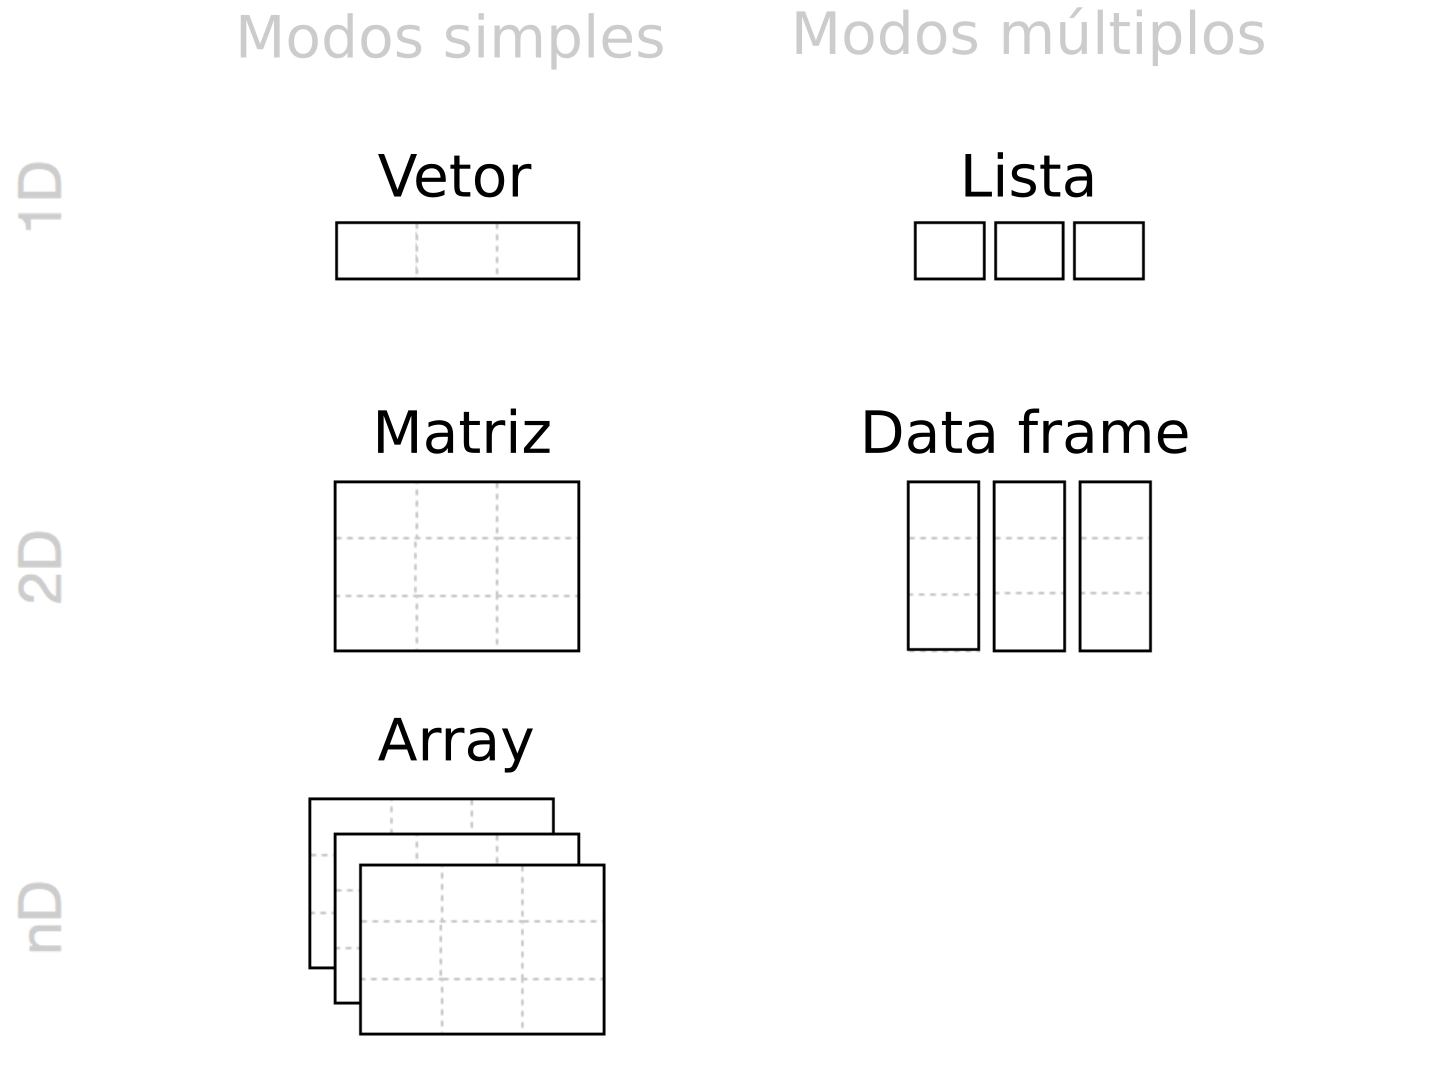
\includegraphics[width=0.7\linewidth]{img/cap04_fig03} 

}

\caption{Estruturas de dados mais comuns de R: vetores, matrizes, arrays, listas e data frames. Adaptado de: @grolemund2014.}\label{fig:fig-r-estruturas}
\end{figure}

\hypertarget{vetor}{%
\paragraph{Vetor}\label{vetor}}

Vetores representam o encadeamento de elementos numa sequência unidimensional. No Capítulo \ref{cap3}, vimos o conceito de variável aleatória e seus tipos. No R, essas variáveis podem ser operacionalizadas como vetores. Dessa forma, essa estrutura de dados pode ser traduzida como medidas de uma variável numérica (discretas ou contínuas), variável binária (booleana - TRUE e FALSE) ou descrição (informações em texto).

Há diversas formas de se criar um vetor no R:

\begin{enumerate}
\def\labelenumi{\arabic{enumi}.}
\tightlist
\item
  Concatenando elementos com a função \texttt{c()}
\item
  Criando sequências unitárias \texttt{:} ou com a função \texttt{seq()}
\item
  Criando repetições com a função \texttt{rep()}
\item
  ``Colar'' palavras com uma sequência numérica com a função \texttt{paste()} ou \texttt{paste0()}
\item
  Amostrando aleatoriamente elementos com a função \texttt{sample()}
\end{enumerate}

\begin{Shaded}
\begin{Highlighting}[]
\DocumentationTok{\#\# Concatenar elementos numéricos}
\NormalTok{concatenar }\OtherTok{\textless{}{-}} \FunctionTok{c}\NormalTok{(}\DecValTok{15}\NormalTok{, }\DecValTok{18}\NormalTok{, }\DecValTok{20}\NormalTok{, }\DecValTok{22}\NormalTok{, }\DecValTok{18}\NormalTok{)}
\NormalTok{concatenar}
\CommentTok{\#\textgreater{} [1] 15 18 20 22 18}

\DocumentationTok{\#\# Sequência unitária (x1:x2)}
\NormalTok{sequencia }\OtherTok{\textless{}{-}} \DecValTok{1}\SpecialCharTok{:}\DecValTok{10}
\NormalTok{sequencia}
\CommentTok{\#\textgreater{}  [1]  1  2  3  4  5  6  7  8  9 10}

\DocumentationTok{\#\# Sequência com diferentes espaçamentos }
\NormalTok{sequencia\_esp }\OtherTok{\textless{}{-}} \FunctionTok{seq}\NormalTok{(}\AttributeTok{from =} \DecValTok{0}\NormalTok{, }\AttributeTok{to =} \DecValTok{100}\NormalTok{, }\AttributeTok{by =} \DecValTok{10}\NormalTok{) }
\NormalTok{sequencia\_esp}
\CommentTok{\#\textgreater{}  [1]   0  10  20  30  40  50  60  70  80  90 100}

\DocumentationTok{\#\# Repetição}
\NormalTok{repeticao }\OtherTok{\textless{}{-}} \FunctionTok{rep}\NormalTok{(}\AttributeTok{x =} \FunctionTok{c}\NormalTok{(}\ConstantTok{TRUE}\NormalTok{, }\ConstantTok{FALSE}\NormalTok{), }\AttributeTok{times =} \DecValTok{5}\NormalTok{)}
\NormalTok{repeticao}
\CommentTok{\#\textgreater{}  [1]  TRUE FALSE  TRUE FALSE  TRUE FALSE  TRUE FALSE  TRUE FALSE}

\DocumentationTok{\#\# Cola palavra e sequência numérica}
\NormalTok{colar }\OtherTok{\textless{}{-}} \FunctionTok{paste}\NormalTok{(}\StringTok{"amostra"}\NormalTok{, }\DecValTok{1}\SpecialCharTok{:}\DecValTok{5}\NormalTok{)}
\NormalTok{colar}
\CommentTok{\#\textgreater{} [1] "amostra 1" "amostra 2" "amostra 3" "amostra 4" "amostra 5"}

\DocumentationTok{\#\# Amostragem aleatória}
\NormalTok{amostragem }\OtherTok{\textless{}{-}} \FunctionTok{sample}\NormalTok{(}\AttributeTok{x =} \DecValTok{1}\SpecialCharTok{:}\DecValTok{100}\NormalTok{, }\AttributeTok{size =} \DecValTok{10}\NormalTok{)}
\NormalTok{amostragem}
\CommentTok{\#\textgreater{}  [1] 45 23 76 63 47 31 68 73 69  5}
\end{Highlighting}
\end{Shaded}

Como os vetores são homogêneos, i.e., só comportam um modo, quando combinamos mais de um modo no mesmo objeto ocorre uma dominância de modos. Existe, dessa forma, uma \textbf{coerção} dos elementos combinados para que todos fiquem iguais. Essa dominância segue essa ordem:

\begin{quote}
\textbf{\texttt{DOMINANTE}} character \textgreater{} double \textgreater{} integer \textgreater{} logical \textbf{\texttt{RECESSIVO}}
\end{quote}

Além disso, podemos utilizar as conversões listadas anteriormente para alterar os modos. Vamos exemplificar combinando os vetores criados anteriormente e convertendo-os.

\begin{Shaded}
\begin{Highlighting}[]
\DocumentationTok{\#\# Coerção}
\FunctionTok{c}\NormalTok{(colar, amostragem)}
\CommentTok{\#\textgreater{}  [1] "amostra 1" "amostra 2" "amostra 3" "amostra 4" "amostra 5" "45"       }
\CommentTok{\#\textgreater{}  [7] "23"        "76"        "63"        "47"        "31"        "68"       }
\CommentTok{\#\textgreater{} [13] "73"        "69"        "5"}

\DocumentationTok{\#\# Conversão}
\FunctionTok{as.numeric}\NormalTok{(repeticao)}
\CommentTok{\#\textgreater{}  [1] 1 0 1 0 1 0 1 0 1 0}
\end{Highlighting}
\end{Shaded}

\hypertarget{fator}{%
\paragraph{Fator}\label{fator}}

O fator representa medidas de uma variável categórica, podendo ser nominal ou ordinal. É fundamental destacar que fatores no R devem ser entendidos como um vetor de \textbf{integer}, i.e., ele é composto por números inteiros representando os níveis da variável categórica.

Para criar um fator no R usamos uma função específica \texttt{factor()}, na qual podemos especificar os \textbf{níveis} com o argumento \texttt{level}, ou fazemos uma conversão usando a função \texttt{as.factor()}. Trabalhar com fatores no \emph{R Base} não é das tarefas mais agradáveis, sendo assim, no Capítulo \ref{cap05} usamos a versão \emph{tidyverse} usando o pacote \texttt{forcats}.

\begin{Shaded}
\begin{Highlighting}[]
\DocumentationTok{\#\# Fator nominal}
\NormalTok{fator\_nominal }\OtherTok{\textless{}{-}} \FunctionTok{factor}\NormalTok{(}\AttributeTok{x =} \FunctionTok{sample}\NormalTok{(}\AttributeTok{x =} \FunctionTok{c}\NormalTok{(}\StringTok{"floresta"}\NormalTok{, }\StringTok{"pastagem"}\NormalTok{, }\StringTok{"cerrado"}\NormalTok{), }
                                   \AttributeTok{size =} \DecValTok{20}\NormalTok{, }\AttributeTok{replace =} \ConstantTok{TRUE}\NormalTok{),}
                        \AttributeTok{levels =} \FunctionTok{c}\NormalTok{(}\StringTok{"floresta"}\NormalTok{, }\StringTok{"pastagem"}\NormalTok{, }\StringTok{"cerrado"}\NormalTok{))}
\NormalTok{fator\_nominal}
\CommentTok{\#\textgreater{}  [1] cerrado  cerrado  floresta pastagem pastagem cerrado  cerrado  pastagem}
\CommentTok{\#\textgreater{}  [9] cerrado  floresta floresta floresta pastagem pastagem cerrado  cerrado }
\CommentTok{\#\textgreater{} [17] pastagem cerrado  floresta pastagem}
\CommentTok{\#\textgreater{} Levels: floresta pastagem cerrado}

\DocumentationTok{\#\# Fator ordinal}
\NormalTok{fator\_ordinal }\OtherTok{\textless{}{-}} \FunctionTok{factor}\NormalTok{(}\AttributeTok{x =} \FunctionTok{sample}\NormalTok{(}\AttributeTok{x =} \FunctionTok{c}\NormalTok{(}\StringTok{"baixa"}\NormalTok{, }\StringTok{"media"}\NormalTok{, }\StringTok{"alta"}\NormalTok{), }
                                   \AttributeTok{size =} \DecValTok{20}\NormalTok{, }\AttributeTok{replace =} \ConstantTok{TRUE}\NormalTok{),}
                        \AttributeTok{levels =} \FunctionTok{c}\NormalTok{(}\StringTok{"baixa"}\NormalTok{, }\StringTok{"media"}\NormalTok{, }\StringTok{"alta"}\NormalTok{), }\AttributeTok{ordered =} \ConstantTok{TRUE}\NormalTok{)}
\NormalTok{fator\_ordinal}
\CommentTok{\#\textgreater{}  [1] alta  alta  baixa media baixa media alta  media baixa media baixa media}
\CommentTok{\#\textgreater{} [13] alta  baixa media media alta  media baixa baixa}
\CommentTok{\#\textgreater{} Levels: baixa \textless{} media \textless{} alta}

\DocumentationTok{\#\# Conversão}
\NormalTok{fator }\OtherTok{\textless{}{-}} \FunctionTok{as.factor}\NormalTok{(}\AttributeTok{x =} \FunctionTok{sample}\NormalTok{(}\AttributeTok{x =} \FunctionTok{c}\NormalTok{(}\StringTok{"floresta"}\NormalTok{, }\StringTok{"pastagem"}\NormalTok{, }\StringTok{"cerrado"}\NormalTok{), }
                              \AttributeTok{size =} \DecValTok{20}\NormalTok{, }\AttributeTok{replace =} \ConstantTok{TRUE}\NormalTok{))}
\NormalTok{fator}
\CommentTok{\#\textgreater{}  [1] cerrado  pastagem floresta floresta cerrado  cerrado  pastagem cerrado }
\CommentTok{\#\textgreater{}  [9] pastagem cerrado  pastagem cerrado  pastagem pastagem floresta cerrado }
\CommentTok{\#\textgreater{} [17] pastagem pastagem cerrado  floresta}
\CommentTok{\#\textgreater{} Levels: cerrado floresta pastagem}
\end{Highlighting}
\end{Shaded}

\hypertarget{matriz}{%
\paragraph{Matriz}\label{matriz}}

A matriz representa dados no formato de tabela, com linhas e colunas. As linhas representam unidades amostrais (locais, transectos, parcelas) e as colunas representam variáveis numéricas (discretas ou contínuas), variáveis binárias (TRUE ou FALSE) ou descrições (informações em texto).

Podemos criar matrizes no R de duas formas. A primeira delas dispondo elementos de um vetor em um certo número de linhas e colunas com a função \texttt{matrix()}, podendo preencher essa matriz com os elementos do vetor por linhas ou por colunas alterando o argumento \texttt{byrow}.

\begin{Shaded}
\begin{Highlighting}[]
\DocumentationTok{\#\# Vetor}
\NormalTok{ve }\OtherTok{\textless{}{-}} \DecValTok{1}\SpecialCharTok{:}\DecValTok{12}

\DocumentationTok{\#\# Matrix {-} preenchimento por linhas {-} horizontal}
\NormalTok{ma\_row }\OtherTok{\textless{}{-}} \FunctionTok{matrix}\NormalTok{(}\AttributeTok{data =}\NormalTok{ ve, }\AttributeTok{nrow =} \DecValTok{4}\NormalTok{, }\AttributeTok{ncol =} \DecValTok{3}\NormalTok{, }\AttributeTok{byrow =} \ConstantTok{TRUE}\NormalTok{)}
\NormalTok{ma\_row}
\CommentTok{\#\textgreater{}      [,1] [,2] [,3]}
\CommentTok{\#\textgreater{} [1,]    1    2    3}
\CommentTok{\#\textgreater{} [2,]    4    5    6}
\CommentTok{\#\textgreater{} [3,]    7    8    9}
\CommentTok{\#\textgreater{} [4,]   10   11   12}

\DocumentationTok{\#\# Matrix {-} preenchimento por colunas {-} vertical}
\NormalTok{ma\_col }\OtherTok{\textless{}{-}} \FunctionTok{matrix}\NormalTok{(}\AttributeTok{data =}\NormalTok{ ve, }\AttributeTok{nrow =} \DecValTok{4}\NormalTok{, }\AttributeTok{ncol =} \DecValTok{3}\NormalTok{, }\AttributeTok{byrow =} \ConstantTok{FALSE}\NormalTok{)}
\NormalTok{ma\_col}
\CommentTok{\#\textgreater{}      [,1] [,2] [,3]}
\CommentTok{\#\textgreater{} [1,]    1    5    9}
\CommentTok{\#\textgreater{} [2,]    2    6   10}
\CommentTok{\#\textgreater{} [3,]    3    7   11}
\CommentTok{\#\textgreater{} [4,]    4    8   12}
\end{Highlighting}
\end{Shaded}

A segundo forma, combinando vetores, utilizando a função \texttt{rbind()} para combinar vetores por linha, i.e., vetor embaixo do outro, e \texttt{cbind()} para combinar vetores por coluna, i.e., vetor ao lado do outro.

\begin{Shaded}
\begin{Highlighting}[]
\DocumentationTok{\#\# Criar dois vetores}
\NormalTok{vec\_1 }\OtherTok{\textless{}{-}} \FunctionTok{c}\NormalTok{(}\DecValTok{1}\NormalTok{, }\DecValTok{2}\NormalTok{, }\DecValTok{3}\NormalTok{)}
\NormalTok{vec\_2 }\OtherTok{\textless{}{-}} \FunctionTok{c}\NormalTok{(}\DecValTok{4}\NormalTok{, }\DecValTok{5}\NormalTok{, }\DecValTok{6}\NormalTok{)}

\DocumentationTok{\#\# Combinar por linhas {-} vertical {-} um embaixo do outro}
\NormalTok{ma\_rbind }\OtherTok{\textless{}{-}} \FunctionTok{rbind}\NormalTok{(vec\_1, vec\_2)}
\NormalTok{ma\_rbind}
\CommentTok{\#\textgreater{}       [,1] [,2] [,3]}
\CommentTok{\#\textgreater{} vec\_1    1    2    3}
\CommentTok{\#\textgreater{} vec\_2    4    5    6}

\DocumentationTok{\#\# Combinar por colunas {-} horizontal {-} um ao lado do outro}
\NormalTok{ma\_cbind }\OtherTok{\textless{}{-}} \FunctionTok{cbind}\NormalTok{(vec\_1, vec\_2)}
\NormalTok{ma\_cbind}
\CommentTok{\#\textgreater{}      vec\_1 vec\_2}
\CommentTok{\#\textgreater{} [1,]     1     4}
\CommentTok{\#\textgreater{} [2,]     2     5}
\CommentTok{\#\textgreater{} [3,]     3     6}
\end{Highlighting}
\end{Shaded}

\hypertarget{array}{%
\paragraph{Array}\label{array}}

O array representa combinação de tabelas, com linhas, colunas e dimensões. Essa combinação pode ser feita em múltiplas dimensões, mas apesar disso, geralmente é mais comum o uso em Ecologia para três dimensões, por exemplo: linhas (unidades amostrais), colunas (espécies) e dimensão (tempo). Isso gera um ``cubo mágico'' ou ``cartas de um baralho'', onde podemos comparar, nesse caso, comunidades ao longo do tempo. Além disso, arrays também são muito comuns em morfometria geométrica ou sensoriamento remoto.

Podemos criar arrays no R dispondo elementos de um vetor em um certo número de linhas, colunas e dimensões com a função \texttt{array()}. Em nosso exemplo, vamos compor cinco comunidades de cinco espécies ao longo de três períodos.

\begin{Shaded}
\begin{Highlighting}[]
\DocumentationTok{\#\# Array}
\NormalTok{ar }\OtherTok{\textless{}{-}} \FunctionTok{array}\NormalTok{(}\AttributeTok{data =} \FunctionTok{sample}\NormalTok{(}\AttributeTok{x =} \FunctionTok{c}\NormalTok{(}\DecValTok{0}\NormalTok{, }\DecValTok{1}\NormalTok{), }\AttributeTok{size =} \DecValTok{75}\NormalTok{, }\AttributeTok{rep =} \ConstantTok{TRUE}\NormalTok{), }
            \AttributeTok{dim =} \FunctionTok{c}\NormalTok{(}\DecValTok{5}\NormalTok{, }\DecValTok{5}\NormalTok{, }\DecValTok{3}\NormalTok{))}
\NormalTok{ar}
\CommentTok{\#\textgreater{} , , 1}
\CommentTok{\#\textgreater{} }
\CommentTok{\#\textgreater{}      [,1] [,2] [,3] [,4] [,5]}
\CommentTok{\#\textgreater{} [1,]    1    0    1    1    0}
\CommentTok{\#\textgreater{} [2,]    1    0    1    1    0}
\CommentTok{\#\textgreater{} [3,]    1    1    1    1    1}
\CommentTok{\#\textgreater{} [4,]    0    1    0    1    0}
\CommentTok{\#\textgreater{} [5,]    1    0    1    0    0}
\CommentTok{\#\textgreater{} }
\CommentTok{\#\textgreater{} , , 2}
\CommentTok{\#\textgreater{} }
\CommentTok{\#\textgreater{}      [,1] [,2] [,3] [,4] [,5]}
\CommentTok{\#\textgreater{} [1,]    0    0    0    1    0}
\CommentTok{\#\textgreater{} [2,]    0    1    0    1    0}
\CommentTok{\#\textgreater{} [3,]    1    1    1    1    0}
\CommentTok{\#\textgreater{} [4,]    0    0    0    0    1}
\CommentTok{\#\textgreater{} [5,]    0    0    0    0    0}
\CommentTok{\#\textgreater{} }
\CommentTok{\#\textgreater{} , , 3}
\CommentTok{\#\textgreater{} }
\CommentTok{\#\textgreater{}      [,1] [,2] [,3] [,4] [,5]}
\CommentTok{\#\textgreater{} [1,]    0    1    1    1    1}
\CommentTok{\#\textgreater{} [2,]    0    0    0    0    0}
\CommentTok{\#\textgreater{} [3,]    0    1    1    1    1}
\CommentTok{\#\textgreater{} [4,]    0    0    1    0    0}
\CommentTok{\#\textgreater{} [5,]    0    1    0    1    0}
\end{Highlighting}
\end{Shaded}

\hypertarget{data-frame}{%
\paragraph{Data frame}\label{data-frame}}

O data frame também representa dados no formato de tabela, com linhas e colunas, muito semelhante à matriz. Mas diferentemente das matrizes, os data frames comportam mais de um modo em suas colunas. Dessa forma, as linhas do data frame ainda representam unidades amostrais (locais, transectos, parcelas), mas as colunas agora podem representar descrições (informações em texto), variáveis numéricas (discretas ou contínuas), variáveis binárias (TRUE ou FALSE) e variáveis categóricas (nominais ou ordinais).

A forma mais simples de criar data frames no R é através da combinação de vetores. Essa combinação é feita com a função \texttt{data.frame()} e ocorre de forma horizontal, semelhante à função \texttt{cbind()}. Sendo assim, todos os vetores precisam ter o mesmo número de elementos, ou seja, o mesmo comprimento. Podemos ainda nomear as colunas de cada vetor.

\begin{Shaded}
\begin{Highlighting}[]
\DocumentationTok{\#\# Criar três vetores}
\NormalTok{vec\_ch }\OtherTok{\textless{}{-}} \FunctionTok{c}\NormalTok{(}\StringTok{"sp1"}\NormalTok{, }\StringTok{"sp2"}\NormalTok{, }\StringTok{"sp3"}\NormalTok{)}
\NormalTok{vec\_nu }\OtherTok{\textless{}{-}} \FunctionTok{c}\NormalTok{(}\DecValTok{4}\NormalTok{, }\DecValTok{5}\NormalTok{, }\DecValTok{6}\NormalTok{)}
\NormalTok{vec\_fa }\OtherTok{\textless{}{-}} \FunctionTok{factor}\NormalTok{(}\FunctionTok{c}\NormalTok{(}\StringTok{"campo"}\NormalTok{, }\StringTok{"floresta"}\NormalTok{, }\StringTok{"floresta"}\NormalTok{))}

\DocumentationTok{\#\# Data frame {-} combinar por colunas {-} horizontal {-} um ao lado do outro}
\NormalTok{df }\OtherTok{\textless{}{-}} \FunctionTok{data.frame}\NormalTok{(vec\_ch, vec\_nu, vec\_fa)}

\NormalTok{df}
\CommentTok{\#\textgreater{}   vec\_ch vec\_nu   vec\_fa}
\CommentTok{\#\textgreater{} 1    sp1      4    campo}
\CommentTok{\#\textgreater{} 2    sp2      5 floresta}
\CommentTok{\#\textgreater{} 3    sp3      6 floresta}

\DocumentationTok{\#\# Data frame {-} nomear as colunas}
\NormalTok{df }\OtherTok{\textless{}{-}} \FunctionTok{data.frame}\NormalTok{(}\AttributeTok{especies =}\NormalTok{ vec\_ch, }
                 \AttributeTok{abundancia =}\NormalTok{ vec\_nu, }
                 \AttributeTok{vegetacao =}\NormalTok{ vec\_fa)}
\NormalTok{df}
\CommentTok{\#\textgreater{}   especies abundancia vegetacao}
\CommentTok{\#\textgreater{} 1      sp1          4     campo}
\CommentTok{\#\textgreater{} 2      sp2          5  floresta}
\CommentTok{\#\textgreater{} 3      sp3          6  floresta}
\end{Highlighting}
\end{Shaded}

\hypertarget{lista}{%
\paragraph{Lista}\label{lista}}

A lista é um tipo especial de vetor que aceita objetos como elementos. Ela é a estrutura de dados utilizada para agrupar objetos, e é geralmente a saída de muitas funções.

Podemos criar listas através da função \texttt{list()}. Essa função funciona de forma semelhante à função \texttt{c()} para a criação de vetores, mas agora estamos concatenando objetos. Podemos ainda nomear os elementos (objetos) que estamos combinando.

Um ponto interessante para entender data frames, é que eles são listas, em que todos os elementos (colunas) possuem o mesmo número de elementos, ou seja, mesmo comprimento.

\begin{Shaded}
\begin{Highlighting}[]
\DocumentationTok{\#\# Lista}
\NormalTok{lista }\OtherTok{\textless{}{-}} \FunctionTok{list}\NormalTok{(}\FunctionTok{rep}\NormalTok{(}\DecValTok{1}\NormalTok{, }\DecValTok{20}\NormalTok{), }\CommentTok{\# vector}
              \FunctionTok{factor}\NormalTok{(}\DecValTok{1}\NormalTok{, }\DecValTok{1}\NormalTok{), }\CommentTok{\# factor}
              \FunctionTok{cbind}\NormalTok{(}\FunctionTok{c}\NormalTok{(}\DecValTok{1}\NormalTok{, }\DecValTok{2}\NormalTok{), }\FunctionTok{c}\NormalTok{(}\DecValTok{1}\NormalTok{, }\DecValTok{2}\NormalTok{))) }\CommentTok{\# matrix}
\NormalTok{lista}
\CommentTok{\#\textgreater{} [[1]]}
\CommentTok{\#\textgreater{}  [1] 1 1 1 1 1 1 1 1 1 1 1 1 1 1 1 1 1 1 1 1}
\CommentTok{\#\textgreater{} }
\CommentTok{\#\textgreater{} [[2]]}
\CommentTok{\#\textgreater{} [1] 1}
\CommentTok{\#\textgreater{} Levels: 1}
\CommentTok{\#\textgreater{} }
\CommentTok{\#\textgreater{} [[3]]}
\CommentTok{\#\textgreater{}      [,1] [,2]}
\CommentTok{\#\textgreater{} [1,]    1    1}
\CommentTok{\#\textgreater{} [2,]    2    2}

\DocumentationTok{\#\# Lista {-} nomear os elementos}
\NormalTok{lista\_nome }\OtherTok{\textless{}{-}} \FunctionTok{list}\NormalTok{(}\AttributeTok{vector =} \FunctionTok{rep}\NormalTok{(}\DecValTok{1}\NormalTok{, }\DecValTok{20}\NormalTok{), }\CommentTok{\# vector}
              \AttributeTok{factor =} \FunctionTok{factor}\NormalTok{(}\DecValTok{1}\NormalTok{, }\DecValTok{1}\NormalTok{), }\CommentTok{\# factor}
              \AttributeTok{matrix =} \FunctionTok{cbind}\NormalTok{(}\FunctionTok{c}\NormalTok{(}\DecValTok{1}\NormalTok{, }\DecValTok{2}\NormalTok{), }\FunctionTok{c}\NormalTok{(}\DecValTok{1}\NormalTok{, }\DecValTok{2}\NormalTok{))) }\CommentTok{\# matrix}
\NormalTok{lista\_nome}
\CommentTok{\#\textgreater{} $vector}
\CommentTok{\#\textgreater{}  [1] 1 1 1 1 1 1 1 1 1 1 1 1 1 1 1 1 1 1 1 1}
\CommentTok{\#\textgreater{} }
\CommentTok{\#\textgreater{} $factor}
\CommentTok{\#\textgreater{} [1] 1}
\CommentTok{\#\textgreater{} Levels: 1}
\CommentTok{\#\textgreater{} }
\CommentTok{\#\textgreater{} $matrix}
\CommentTok{\#\textgreater{}      [,1] [,2]}
\CommentTok{\#\textgreater{} [1,]    1    1}
\CommentTok{\#\textgreater{} [2,]    2    2}
\end{Highlighting}
\end{Shaded}

\hypertarget{funuxe7uxf5es-1}{%
\paragraph{Funções}\label{funuxe7uxf5es-1}}

Uma última estrutura de objetos criados no R são as funções. Elas são objetos criados pelo usuário e reutilizados para fazer operações específicas. A criação de funções geralmente é um tópico tratado num segundo momento, quando o usuário de R adquire certo conhecimento da linguagem. Aqui abordaremos apenas seu funcionamento básico, diferenciando sua estrutura para entendimento e sua diferenciação das demais estruturas.

Vamos criar uma função simples que retorna a multiplicação de dois termos. Criaremos a função com o nome \texttt{multi}, à qual será atribuída uma função com o nome \texttt{function()}, com dois argumentos \texttt{x} e \texttt{y}. Depois disso abrimos chaves \texttt{\{\}}, que é onde iremos incluir nosso bloco de código. Nosso bloco de código é composto por duas linhas, a primeira contendo a operação de multiplicação dos argumento com a atribuição ao objeto \texttt{mu} e a sugunda contendo a função \texttt{return()} para retornar o valor da multiplicação.

\begin{Shaded}
\begin{Highlighting}[]
\DocumentationTok{\#\# Criar uma função}
\NormalTok{multi }\OtherTok{\textless{}{-}} \ControlFlowTok{function}\NormalTok{(x, y)\{}
  
\NormalTok{  mu }\OtherTok{\textless{}{-}}\NormalTok{ (x }\SpecialCharTok{*}\NormalTok{ y)}
  \FunctionTok{return}\NormalTok{(mu)}
 
\NormalTok{\}}
\NormalTok{multi}
\CommentTok{\#\textgreater{} function(x, y)\{}
\CommentTok{\#\textgreater{}   }
\CommentTok{\#\textgreater{}   mu \textless{}{-} (x * y)}
\CommentTok{\#\textgreater{}   return(mu)}
\CommentTok{\#\textgreater{}  }
\CommentTok{\#\textgreater{} \}}

\DocumentationTok{\#\# Uso da função}
\FunctionTok{multi}\NormalTok{(}\DecValTok{42}\NormalTok{, }\DecValTok{42}\NormalTok{)}
\CommentTok{\#\textgreater{} [1] 1764}
\end{Highlighting}
\end{Shaded}

\hypertarget{manipulauxe7uxe3o-de-objetos-unidimensionais}{%
\subsection{Manipulação de objetos unidimensionais}\label{manipulauxe7uxe3o-de-objetos-unidimensionais}}

Vamos agora explorar formas de manipular elementos de objetos unidimensionais, ou seja, vetores, fatores e listas.

A primeira forma de manipulação é através da \textbf{indexação}, utilizando os operadores \texttt{{[}{]}}. Com a indexação podemos acessar elementos de vetores e fatores por sua posição. Utilizaremos números, sequência de números ou operações booleanas para retornar partes dos vetores ou fatores. Podemos ainda retirar elementos dessas estruturas com o operador aritmético \texttt{-}.

No exemplo a seguir, iremos fixar o ponto de partida da amostragem da função \texttt{sample()}, utilizando a função \texttt{set.seed(42)} (usamos 42 porque é a resposta para a vida, o universo e tudo mais - O Guia do Mochileiro das Galáxias, mas poderia ser outro número qualquer). Isso permite que o resultado da amostragem aleatório seja igual em diferentes computadores.

\begin{Shaded}
\begin{Highlighting}[]
\DocumentationTok{\#\# Fixar a amostragem}
\FunctionTok{set.seed}\NormalTok{(}\DecValTok{42}\NormalTok{)}

\DocumentationTok{\#\# Amostrar 10 elementos de uma sequência}
\NormalTok{ve }\OtherTok{\textless{}{-}} \FunctionTok{sample}\NormalTok{(}\AttributeTok{x =} \FunctionTok{seq}\NormalTok{(}\DecValTok{0}\NormalTok{, }\DecValTok{2}\NormalTok{, .}\DecValTok{05}\NormalTok{), }\AttributeTok{size =} \DecValTok{10}\NormalTok{)}
\NormalTok{ve}
\CommentTok{\#\textgreater{}  [1] 1.80 0.00 1.20 0.45 1.75 0.85 1.15 0.30 1.90 0.20}

\DocumentationTok{\#\# Seleciona o quinto elemento}
\NormalTok{ve[}\DecValTok{5}\NormalTok{]}
\CommentTok{\#\textgreater{} [1] 1.75}

\DocumentationTok{\#\# Seleciona os elementos de 1 a 5}
\NormalTok{ve[}\DecValTok{1}\SpecialCharTok{:}\DecValTok{5}\NormalTok{]}
\CommentTok{\#\textgreater{} [1] 1.80 0.00 1.20 0.45 1.75}

\DocumentationTok{\#\# Retira o decimo elemento}
\NormalTok{ve[}\SpecialCharTok{{-}}\DecValTok{10}\NormalTok{]}
\CommentTok{\#\textgreater{} [1] 1.80 0.00 1.20 0.45 1.75 0.85 1.15 0.30 1.90}

\DocumentationTok{\#\# Retira os elementos 2 a 9}
\NormalTok{ve[}\SpecialCharTok{{-}}\NormalTok{(}\DecValTok{2}\SpecialCharTok{:}\DecValTok{9}\NormalTok{)]}
\CommentTok{\#\textgreater{} [1] 1.8 0.2}
\end{Highlighting}
\end{Shaded}

Podemos ainda fazer uma seleção condicional do vetor. Ao utilizarmos operadores relacionais, teremos como resposta um vetor lógico. Esse vetor lógico pode ser utilizado dentro da indexação para seleção de elementos.

\begin{Shaded}
\begin{Highlighting}[]
\DocumentationTok{\#\# Quais valores sao maiores que 1?}
\NormalTok{ve }\SpecialCharTok{\textgreater{}} \DecValTok{1}
\CommentTok{\#\textgreater{}  [1]  TRUE FALSE  TRUE FALSE  TRUE FALSE  TRUE FALSE  TRUE FALSE}

\DocumentationTok{\#\# Valores acima de 1}
\NormalTok{ve[ve }\SpecialCharTok{\textgreater{}} \DecValTok{1}\NormalTok{]}
\CommentTok{\#\textgreater{} [1] 1.80 1.20 1.75 1.15 1.90}
\end{Highlighting}
\end{Shaded}

Além da indexação, temos algumas funções que nos auxiliam em algumas operações com objetos unidimensionais, listadas na Tabela \ref{tab:tab-tab-funcoes-conf-uni}.

\begin{table}

\caption{\label{tab:tab-tab-funcoes-conf-uni}Funções para verificação e resumo de dados unidimensionais.}
\centering
\begin{tabular}[t]{c|c}
\hline
Função & Descrição\\
\hline
`max()` & Valor máximo\\
\hline
`min()` & Valor mínimo\\
\hline
`range()` & Amplitude\\
\hline
`length()` & Comprimento\\
\hline
`sum()` & Soma\\
\hline
`cumsum()` & Soma cumulativa\\
\hline
`prod()` & Produto\\
\hline
`sqrt()` & Raiz quadrada\\
\hline
`abs()` & Valor absoluto\\
\hline
`exp()` & Expoente\\
\hline
`log()` & Logaritmo natural\\
\hline
`log1p()` & Logaritmo natural mais 1 *log(x + 1)*\\
\hline
`log2()` & Logaritmo base 2\\
\hline
`log10()` & Logaritmo base 10\\
\hline
`mean()` & Média\\
\hline
`mean.weighted()` & Média ponderada\\
\hline
`var()` & Variância\\
\hline
`sd()` & Desvio Padrão\\
\hline
`mediam()` & Mediana\\
\hline
`quantile()` & Quantil\\
\hline
`quarters()` & Quartil\\
\hline
`IQR()` & Amplitude interquartil\\
\hline
`round()` & Arredondamento\\
\hline
`sort()` & Ordenação\\
\hline
`order()` & Posição ordenada\\
\hline
`rev()` & Reverso\\
\hline
`unique()` & Únicos\\
\hline
`summary()` & Resumo estatístico\\
\hline
`cut()` & Divide variável contínua em fator\\
\hline
`pretty()` & Divide variável contínua em intervalos\\
\hline
`scale()` & Padronização e centralização\\
\hline
`sub()` & Substitui caracteres\\
\hline
`grep()` & Posição de caracteres\\
\hline
`any()` & Algum valor?\\
\hline
`all()` & Todos os valores?\\
\hline
`which()` & Quais valores?\\
\hline
`subset()` & Subconjunto\\
\hline
`ifelse()` & Operação condicional\\
\hline
\end{tabular}
\end{table}

Para listas, também podemos usar a indexação \texttt{{[}{]}} para acessar ou retirar elementos.

\begin{Shaded}
\begin{Highlighting}[]
\DocumentationTok{\#\# Lista}
\NormalTok{li }\OtherTok{\textless{}{-}} \FunctionTok{list}\NormalTok{(}\AttributeTok{elem1 =} \DecValTok{1}\NormalTok{, }\AttributeTok{elem2 =} \DecValTok{2}\NormalTok{, }\AttributeTok{elem3 =} \DecValTok{3}\NormalTok{)}

\DocumentationTok{\#\# Acessar o primeiro elemento}
\NormalTok{li[}\DecValTok{1}\NormalTok{]}
\CommentTok{\#\textgreater{} $elem1}
\CommentTok{\#\textgreater{} [1] 1}

\DocumentationTok{\#\# Retirar o primeiro elemento}
\NormalTok{li[}\SpecialCharTok{{-}}\DecValTok{1}\NormalTok{]}
\CommentTok{\#\textgreater{} $elem2}
\CommentTok{\#\textgreater{} [1] 2}
\CommentTok{\#\textgreater{} }
\CommentTok{\#\textgreater{} $elem3}
\CommentTok{\#\textgreater{} [1] 3}
\end{Highlighting}
\end{Shaded}

Podemos ainda usar a indexação dupla \texttt{{[}{[}{]}{]}} para acessar os valores desses elementos.

\begin{Shaded}
\begin{Highlighting}[]
\DocumentationTok{\#\# Acessar o valor do primeiro elemento}
\NormalTok{li[[}\DecValTok{1}\NormalTok{]]}
\CommentTok{\#\textgreater{} [1] 1}

\DocumentationTok{\#\# Acessar o valor do segundo elemento}
\NormalTok{li[[}\DecValTok{2}\NormalTok{]]}
\CommentTok{\#\textgreater{} [1] 2}
\end{Highlighting}
\end{Shaded}

Para listas nomeadas, podemos ainda utilizar o operador \texttt{\$} para acessar elementos pelo nome.

\begin{Shaded}
\begin{Highlighting}[]
\DocumentationTok{\#\# Acessar o primeiro elemento}
\NormalTok{li}\SpecialCharTok{$}\NormalTok{elem1}
\CommentTok{\#\textgreater{} [1] 1}
\end{Highlighting}
\end{Shaded}

E ainda podemos utilizar funções para medir o comprimento dessa lista, listar os nomes dos elementos ou ainda renomear os elementos: \texttt{length()} e \texttt{names()}.

\begin{Shaded}
\begin{Highlighting}[]
\DocumentationTok{\#\# Comprimento}
\FunctionTok{length}\NormalTok{(li)}
\CommentTok{\#\textgreater{} [1] 3}

\DocumentationTok{\#\# Nomes}
\FunctionTok{names}\NormalTok{(li)}
\CommentTok{\#\textgreater{} [1] "elem1" "elem2" "elem3"}

\DocumentationTok{\#\# Renomear}
\FunctionTok{names}\NormalTok{(li) }\OtherTok{\textless{}{-}} \FunctionTok{paste0}\NormalTok{(}\StringTok{"elemento0"}\NormalTok{, }\DecValTok{1}\SpecialCharTok{:}\DecValTok{3}\NormalTok{)}
\NormalTok{li}
\CommentTok{\#\textgreater{} $elemento01}
\CommentTok{\#\textgreater{} [1] 1}
\CommentTok{\#\textgreater{} }
\CommentTok{\#\textgreater{} $elemento02}
\CommentTok{\#\textgreater{} [1] 2}
\CommentTok{\#\textgreater{} }
\CommentTok{\#\textgreater{} $elemento03}
\CommentTok{\#\textgreater{} [1] 3}
\end{Highlighting}
\end{Shaded}

\hypertarget{manipulauxe7uxe3o-de-objetos-multidimensionais}{%
\subsection{Manipulação de objetos multidimensionais}\label{manipulauxe7uxe3o-de-objetos-multidimensionais}}

Da mesma forma que para objetos unidimensionais, podemos manipular elementos de objetos multidimensionais, ou seja, matrizes, data frames e arrays.

Novamente, a primeira forma de manipulação é através da indexação, utilizando os operadores \texttt{{[}{]}}. Com a indexação podemos acessar elementos de matrizes, data frames e arrays por sua posição. Podemos ainda retirar elementos dessas estruturas com o operador aritmético \texttt{-}.

Entretanto, agora temos mais de uma dimensão na estruturação dos elementos dentro dos objetos. Assim, utilizamos números, sequência de números ou operação booleanas para retornar partes desses objetos, mas as dimensões têm de ser explicitadas e separadas por \textbf{vírgulas} para acessar linhas e colunas. Essa indexação funciona para matrizes e data frames. Para arrays, especificamos também as dimensões, também separadas por vírgulas para acessar essas dimensões.

\begin{Shaded}
\begin{Highlighting}[]
\DocumentationTok{\#\# Matriz}
\NormalTok{ma }\OtherTok{\textless{}{-}} \FunctionTok{matrix}\NormalTok{(}\DecValTok{1}\SpecialCharTok{:}\DecValTok{12}\NormalTok{, }\DecValTok{4}\NormalTok{, }\DecValTok{3}\NormalTok{)}
\NormalTok{ma}
\CommentTok{\#\textgreater{}      [,1] [,2] [,3]}
\CommentTok{\#\textgreater{} [1,]    1    5    9}
\CommentTok{\#\textgreater{} [2,]    2    6   10}
\CommentTok{\#\textgreater{} [3,]    3    7   11}
\CommentTok{\#\textgreater{} [4,]    4    8   12}

\DocumentationTok{\#\# Indexação}
\NormalTok{ma[}\DecValTok{3}\NormalTok{, ] }\CommentTok{\# linha 3}
\CommentTok{\#\textgreater{} [1]  3  7 11}
\NormalTok{ma[, }\DecValTok{2}\NormalTok{] }\CommentTok{\# coluna 2}
\CommentTok{\#\textgreater{} [1] 5 6 7 8}
\NormalTok{ma[}\DecValTok{1}\NormalTok{, }\DecValTok{2}\NormalTok{] }\CommentTok{\# elemento da linha 1 e coluna 2}
\CommentTok{\#\textgreater{} [1] 5}
\NormalTok{ma[}\DecValTok{1}\NormalTok{, }\DecValTok{1}\SpecialCharTok{:}\DecValTok{2}\NormalTok{] }\CommentTok{\# elementos da linha 1 e coluna 1 e 2}
\CommentTok{\#\textgreater{} [1] 1 5}
\NormalTok{ma[}\DecValTok{1}\NormalTok{, }\FunctionTok{c}\NormalTok{(}\DecValTok{1}\NormalTok{, }\DecValTok{3}\NormalTok{)] }\CommentTok{\# elementos da linha 1 e coluna 1 e 3}
\CommentTok{\#\textgreater{} [1] 1 9}
\NormalTok{ma[}\SpecialCharTok{{-}}\DecValTok{1}\NormalTok{, ] }\CommentTok{\# retirar a linha 1}
\CommentTok{\#\textgreater{}      [,1] [,2] [,3]}
\CommentTok{\#\textgreater{} [1,]    2    6   10}
\CommentTok{\#\textgreater{} [2,]    3    7   11}
\CommentTok{\#\textgreater{} [3,]    4    8   12}
\NormalTok{ma[, }\SpecialCharTok{{-}}\DecValTok{3}\NormalTok{] }\CommentTok{\# retirar a coluna 3}
\CommentTok{\#\textgreater{}      [,1] [,2]}
\CommentTok{\#\textgreater{} [1,]    1    5}
\CommentTok{\#\textgreater{} [2,]    2    6}
\CommentTok{\#\textgreater{} [3,]    3    7}
\CommentTok{\#\textgreater{} [4,]    4    8}
\end{Highlighting}
\end{Shaded}

Para data frames, além de utilizar números e/ou sequências de números dentro do operador \texttt{{[}{]}} simples, assim como podemos utilizar o operador \texttt{{[}{[}{]}{]}} duplo para retornar apenas os valores de uma linha ou uma coluna. Se as colunas estiverem nomeadas, podemos utilizar o nome da coluna de interesse entre aspas dentro dos operadores \texttt{{[}{]}} (retornar coluna) e \texttt{{[}{[}{]}{]}} (retornar apenas os valores), assim como ainda podemos utilizar o operador \texttt{\$} para data frames. Essas últimas operações retornam um vetor, para o qual podemos fazer operações de vetores ou ainda atualizar o valor dessa coluna selecionada ou adicionar outra coluna.

\begin{Shaded}
\begin{Highlighting}[]
\DocumentationTok{\#\# Criar três vetores}
\NormalTok{sp }\OtherTok{\textless{}{-}} \FunctionTok{paste}\NormalTok{(}\StringTok{"sp"}\NormalTok{, }\DecValTok{1}\SpecialCharTok{:}\DecValTok{10}\NormalTok{, }\AttributeTok{sep =} \StringTok{""}\NormalTok{)}
\NormalTok{abu }\OtherTok{\textless{}{-}} \DecValTok{1}\SpecialCharTok{:}\DecValTok{10}
\NormalTok{flo }\OtherTok{\textless{}{-}} \FunctionTok{factor}\NormalTok{(}\FunctionTok{rep}\NormalTok{(}\FunctionTok{c}\NormalTok{(}\StringTok{"campo"}\NormalTok{, }\StringTok{"floresta"}\NormalTok{), }\AttributeTok{each =} \DecValTok{5}\NormalTok{))}

\DocumentationTok{\#\# data frame}
\NormalTok{df }\OtherTok{\textless{}{-}} \FunctionTok{data.frame}\NormalTok{(sp, abu, flo)}
\NormalTok{df}
\CommentTok{\#\textgreater{}      sp abu      flo}
\CommentTok{\#\textgreater{} 1   sp1   1    campo}
\CommentTok{\#\textgreater{} 2   sp2   2    campo}
\CommentTok{\#\textgreater{} 3   sp3   3    campo}
\CommentTok{\#\textgreater{} 4   sp4   4    campo}
\CommentTok{\#\textgreater{} 5   sp5   5    campo}
\CommentTok{\#\textgreater{} 6   sp6   6 floresta}
\CommentTok{\#\textgreater{} 7   sp7   7 floresta}
\CommentTok{\#\textgreater{} 8   sp8   8 floresta}
\CommentTok{\#\textgreater{} 9   sp9   9 floresta}
\CommentTok{\#\textgreater{} 10 sp10  10 floresta}

\DocumentationTok{\#\# [] {-} números}
\NormalTok{df[, }\DecValTok{1}\NormalTok{]}
\CommentTok{\#\textgreater{}  [1] "sp1"  "sp2"  "sp3"  "sp4"  "sp5"  "sp6"  "sp7"  "sp8"  "sp9"  "sp10"}

\DocumentationTok{\#\# [] {-} nome das colunas {-} retorna coluna}
\NormalTok{df[}\StringTok{"flo"}\NormalTok{]}
\CommentTok{\#\textgreater{}         flo}
\CommentTok{\#\textgreater{} 1     campo}
\CommentTok{\#\textgreater{} 2     campo}
\CommentTok{\#\textgreater{} 3     campo}
\CommentTok{\#\textgreater{} 4     campo}
\CommentTok{\#\textgreater{} 5     campo}
\CommentTok{\#\textgreater{} 6  floresta}
\CommentTok{\#\textgreater{} 7  floresta}
\CommentTok{\#\textgreater{} 8  floresta}
\CommentTok{\#\textgreater{} 9  floresta}
\CommentTok{\#\textgreater{} 10 floresta}

\DocumentationTok{\#\# [[]] {-} nome das colunas {-} retorna apenas os valores}
\NormalTok{df[[}\StringTok{"flo"}\NormalTok{]]}
\CommentTok{\#\textgreater{}  [1] campo    campo    campo    campo    campo    floresta floresta floresta}
\CommentTok{\#\textgreater{}  [9] floresta floresta}
\CommentTok{\#\textgreater{} Levels: campo floresta}

\DocumentationTok{\#\# $ funciona apenas para data frame }
\NormalTok{df}\SpecialCharTok{$}\NormalTok{sp}
\CommentTok{\#\textgreater{}  [1] "sp1"  "sp2"  "sp3"  "sp4"  "sp5"  "sp6"  "sp7"  "sp8"  "sp9"  "sp10"}

\DocumentationTok{\#\# Operação de vetors}
\FunctionTok{length}\NormalTok{(df}\SpecialCharTok{$}\NormalTok{abu)}
\CommentTok{\#\textgreater{} [1] 10}

\DocumentationTok{\#\# Converter colunas}
\NormalTok{df}\SpecialCharTok{$}\NormalTok{abu }\OtherTok{\textless{}{-}} \FunctionTok{as.character}\NormalTok{(df}\SpecialCharTok{$}\NormalTok{abu)}
\FunctionTok{mode}\NormalTok{(df}\SpecialCharTok{$}\NormalTok{abu)}
\CommentTok{\#\textgreater{} [1] "character"}

\DocumentationTok{\#\# Adicionar colunas}
\FunctionTok{set.seed}\NormalTok{(}\DecValTok{42}\NormalTok{)}
\NormalTok{df}\SpecialCharTok{$}\NormalTok{abu2 }\OtherTok{\textless{}{-}} \FunctionTok{sample}\NormalTok{(}\AttributeTok{x =} \DecValTok{0}\SpecialCharTok{:}\DecValTok{1}\NormalTok{, }\AttributeTok{size =} \FunctionTok{nrow}\NormalTok{(df), }\AttributeTok{rep =} \ConstantTok{TRUE}\NormalTok{)}
\NormalTok{df}
\CommentTok{\#\textgreater{}      sp abu      flo abu2}
\CommentTok{\#\textgreater{} 1   sp1   1    campo    0}
\CommentTok{\#\textgreater{} 2   sp2   2    campo    0}
\CommentTok{\#\textgreater{} 3   sp3   3    campo    0}
\CommentTok{\#\textgreater{} 4   sp4   4    campo    0}
\CommentTok{\#\textgreater{} 5   sp5   5    campo    1}
\CommentTok{\#\textgreater{} 6   sp6   6 floresta    1}
\CommentTok{\#\textgreater{} 7   sp7   7 floresta    1}
\CommentTok{\#\textgreater{} 8   sp8   8 floresta    1}
\CommentTok{\#\textgreater{} 9   sp9   9 floresta    0}
\CommentTok{\#\textgreater{} 10 sp10  10 floresta    1}
\end{Highlighting}
\end{Shaded}

Podemos ainda fazer seleções condicionais para retornar linhas com valores que temos interesse, semelhante ao uso de filtro de uma planilha eletrônica.

\begin{Shaded}
\begin{Highlighting}[]
\DocumentationTok{\#\# Selecionar linhas de uma matriz ou data frame }
\NormalTok{df[df}\SpecialCharTok{$}\NormalTok{abu }\SpecialCharTok{\textgreater{}} \DecValTok{4}\NormalTok{, ]}
\CommentTok{\#\textgreater{}    sp abu      flo abu2}
\CommentTok{\#\textgreater{} 5 sp5   5    campo    1}
\CommentTok{\#\textgreater{} 6 sp6   6 floresta    1}
\CommentTok{\#\textgreater{} 7 sp7   7 floresta    1}
\CommentTok{\#\textgreater{} 8 sp8   8 floresta    1}
\CommentTok{\#\textgreater{} 9 sp9   9 floresta    0}

\NormalTok{df[df}\SpecialCharTok{$}\NormalTok{flo }\SpecialCharTok{==} \StringTok{"floresta"}\NormalTok{, ]}
\CommentTok{\#\textgreater{}      sp abu      flo abu2}
\CommentTok{\#\textgreater{} 6   sp6   6 floresta    1}
\CommentTok{\#\textgreater{} 7   sp7   7 floresta    1}
\CommentTok{\#\textgreater{} 8   sp8   8 floresta    1}
\CommentTok{\#\textgreater{} 9   sp9   9 floresta    0}
\CommentTok{\#\textgreater{} 10 sp10  10 floresta    1}
\end{Highlighting}
\end{Shaded}

Além disso, há uma série de funções para conferência e manipulação de dados que listamos na Tabela \ref{tab:tab-funcoes-conf-multi}.

\begin{table}

\caption{\label{tab:tab-funcoes-conf-multi}Funções para verificação e resumo de dados multidimensionais.}
\centering
\begin{tabular}[t]{c|c}
\hline
Função & Descrição\\
\hline
`head()` & Mostra as primeiras 6 linhas\\
\hline
`tail()` & Mostra as últimas 6 linhas\\
\hline
`nrow()` & Mostra o número de linhas\\
\hline
`ncol()` & Mostra o número de colunas\\
\hline
`dim()` & Mostra o número de linhas e de colunas\\
\hline
`rownames()` & Mostra os nomes das linhas (locais)\\
\hline
`colnames()` & Mostra os nomes das colunas (variáveis)\\
\hline
`str()` & Mostra as classes de cada coluna (estrutura)\\
\hline
`summary()` & Mostra um resumo dos valores de cada coluna\\
\hline
`rowSums()` & Calcula a soma das linhas (horizontal)\\
\hline
`colSums()` & Calcula a soma das colunas (vertical)\\
\hline
`rowMeans()` & Calcula a média das linhas (horizontal)\\
\hline
`colMeans()` & Calcula a média das colunas (vertical)\\
\hline
`str()` & Mostra a estrutura dos dados\\
\hline
`table()` & Tabulação cruzada\\
\hline
`t()` & Matriz ou data frame transposto\\
\hline
\end{tabular}
\end{table}

\hypertarget{valores-faltantes-e-especiais}{%
\subsection{Valores faltantes e especiais}\label{valores-faltantes-e-especiais}}

Valores faltantes e especiais são valores reservados que representam dados faltantes, indefinições matemáticas, infinitos e objetos nulos.

\begin{enumerate}
\def\labelenumi{\arabic{enumi}.}
\tightlist
\item
  \textbf{NA (\emph{Not Available})}: significa dado faltante ou indisponível
\item
  \textbf{NaN (\emph{Not a Number})}: representa indefinições matemáticas
\item
  \textbf{Inf (\emph{Infinito})}: é um número muito grande ou um limite matemático
\item
  \textbf{NULL \emph{(Nulo})}: representa um objeto nulo, sendo útil para preenchimento em aplicações de programação
\end{enumerate}

\begin{Shaded}
\begin{Highlighting}[]
\DocumentationTok{\#\# Data frame com elemento NA}
\NormalTok{df }\OtherTok{\textless{}{-}} \FunctionTok{data.frame}\NormalTok{(}\AttributeTok{var1 =} \FunctionTok{c}\NormalTok{(}\DecValTok{1}\NormalTok{, }\DecValTok{4}\NormalTok{, }\DecValTok{2}\NormalTok{, }\ConstantTok{NA}\NormalTok{), }\AttributeTok{var2 =} \FunctionTok{c}\NormalTok{(}\DecValTok{1}\NormalTok{, }\DecValTok{4}\NormalTok{, }\DecValTok{5}\NormalTok{, }\DecValTok{2}\NormalTok{))}
\NormalTok{df}
\CommentTok{\#\textgreater{}   var1 var2}
\CommentTok{\#\textgreater{} 1    1    1}
\CommentTok{\#\textgreater{} 2    4    4}
\CommentTok{\#\textgreater{} 3    2    5}
\CommentTok{\#\textgreater{} 4   NA    2}

\DocumentationTok{\#\# Resposta booleana para elementos NA}
\FunctionTok{is.na}\NormalTok{(df)}
\CommentTok{\#\textgreater{}       var1  var2}
\CommentTok{\#\textgreater{} [1,] FALSE FALSE}
\CommentTok{\#\textgreater{} [2,] FALSE FALSE}
\CommentTok{\#\textgreater{} [3,] FALSE FALSE}
\CommentTok{\#\textgreater{} [4,]  TRUE FALSE}

\DocumentationTok{\#\# Algum elemento é NA?}
\FunctionTok{any}\NormalTok{(}\FunctionTok{is.na}\NormalTok{(df))}
\CommentTok{\#\textgreater{} [1] TRUE}

\DocumentationTok{\#\# Remover as linhas com NAs}
\NormalTok{df\_sem\_na }\OtherTok{\textless{}{-}} \FunctionTok{na.omit}\NormalTok{(df)}
\NormalTok{df\_sem\_na}
\CommentTok{\#\textgreater{}   var1 var2}
\CommentTok{\#\textgreater{} 1    1    1}
\CommentTok{\#\textgreater{} 2    4    4}
\CommentTok{\#\textgreater{} 3    2    5}

\DocumentationTok{\#\# Substituir NAs por 0}
\NormalTok{df[}\FunctionTok{is.na}\NormalTok{(df)] }\OtherTok{\textless{}{-}} \DecValTok{0}
\NormalTok{df}
\CommentTok{\#\textgreater{}   var1 var2}
\CommentTok{\#\textgreater{} 1    1    1}
\CommentTok{\#\textgreater{} 2    4    4}
\CommentTok{\#\textgreater{} 3    2    5}
\CommentTok{\#\textgreater{} 4    0    2}

\DocumentationTok{\#\# Desconsiderar os NAs em funções com o argumento rm.na = TRUE}
\FunctionTok{sum}\NormalTok{(}\DecValTok{1}\NormalTok{, }\DecValTok{2}\NormalTok{, }\DecValTok{3}\NormalTok{, }\DecValTok{4}\NormalTok{, }\ConstantTok{NA}\NormalTok{, }\AttributeTok{na.rm =} \ConstantTok{TRUE}\NormalTok{)}
\CommentTok{\#\textgreater{} [1] 10}

\DocumentationTok{\#\# NaN {-} not a number}
\DecValTok{0}\SpecialCharTok{/}\DecValTok{0}
\CommentTok{\#\textgreater{} [1] NaN}
\FunctionTok{log}\NormalTok{(}\SpecialCharTok{{-}}\DecValTok{1}\NormalTok{)}
\CommentTok{\#\textgreater{} [1] NaN}

\DocumentationTok{\#\# Limite matemático}
\DecValTok{1}\SpecialCharTok{/}\DecValTok{0}
\CommentTok{\#\textgreater{} [1] Inf}

\DocumentationTok{\#\# Número grande}
\DecValTok{10}\SpecialCharTok{\^{}}\DecValTok{310}
\CommentTok{\#\textgreater{} [1] Inf}

\DocumentationTok{\#\# Objeto nulo}
\NormalTok{nulo }\OtherTok{\textless{}{-}} \ConstantTok{NULL}
\NormalTok{nulo}
\CommentTok{\#\textgreater{} NULL}
\end{Highlighting}
\end{Shaded}

\hypertarget{diretuxf3rio-de-trabalho}{%
\subsection{Diretório de trabalho}\label{diretuxf3rio-de-trabalho}}

O diretório de trabalho é o endereço da pasta (ou diretório) de onde o R importará ou exportar nossos dados.

Podemos utilizar o próprio RStudio para tal tarefa, indo em \texttt{Session\ \textgreater{}\ Set\ Work\ Directory\ \textgreater{}\ Choose\ Directory...} ou simplesmente utilizar o atalho \texttt{Ctrl\ +\ Shift\ +\ H}.

Podemos ainda utilizar as funções do R para definir o diretório. Para tanto, podemos navegar com o aplicativo de gerenciador de arquivos (e.g., Windows Explorer) até nosso diretório de interesse e copiar o endereço na barra superior. Voltamos para o R e colamos esse endereço entre aspas como um argumento da função \texttt{setwd()}. É fundamental destacar que em Sistemas Operacionais Windows é necessário inverter as barras (\texttt{\textbackslash{}} por \texttt{/}).

Aconselhamos ainda utilizar as funções \texttt{getwd()} para retornar o diretório definido na sessão do R, assim como as funções \texttt{dir()} ou \texttt{list.files()} para listagem dos arquivos no diretório, ambas medidas de conferência do diretório correto.

\begin{Shaded}
\begin{Highlighting}[]
\DocumentationTok{\#\# Definir o diretório de trabalho}
\FunctionTok{setwd}\NormalTok{(}\StringTok{"/home/mude/data/github/livro\_r\_ecologia/dados"}\NormalTok{)}

\DocumentationTok{\#\# Verificar o diretório}
\FunctionTok{getwd}\NormalTok{()}

\DocumentationTok{\#\# Listar os arquivos no diretório}
\FunctionTok{dir}\NormalTok{()}
\FunctionTok{list.files}\NormalTok{()}
\end{Highlighting}
\end{Shaded}

Outra forma de definir o diretório é digitar a tecla \texttt{tab} dentro da função \texttt{setwd("tab")}. Quando apertamos a \texttt{tab} dentro das aspas conseguimos selecionar o diretório manualmente, pois abre-se uma lista de diretório que podemos ir selecionando até chegar no diretório de interesse.

\begin{Shaded}
\begin{Highlighting}[]
\DocumentationTok{\#\# Mudar o diretório com a tecla tab}
\FunctionTok{setwd}\NormalTok{(}\StringTok{"\textasciigrave{}tab\textasciigrave{}"}\NormalTok{)}
\end{Highlighting}
\end{Shaded}

\hypertarget{importar-dados}{%
\subsection{Importar dados}\label{importar-dados}}

Uma das operações mais corriqueiras do R, antes de realizar alguma análise ou plotar um gráfico, é a de importar dados que foram tabulados numa planilha eletrônica e salvos no formato .csv, .txt ou .xlsx. Ao importar esse tipo de dado para o R, o formato que o mesmo assume, se nenhum parâmetro for especificado, é o da classe \texttt{data\ frame}, prevendo que a planilha de dados possua colunas com diferentes modos.

Existem diversas formas de importar dados para o R. Podemos importar utilizando o RStudio, indo na janela \textbf{Environment} (Figura \ref{fig:fig-rstudio} (3)) e clicar em ``Importar Dataset''.

Entretanto, aconselhamos o uso de funções que fiquem salvas em um script para aumentar a reprodutibilidade do mesmo. Dessa forma, as três principais funções para importar os arquivos nos três principais extensões (.csv, .txt ou .xlsx) são, respectivamente: \texttt{read.csv()}, \texttt{read.table()} e \texttt{openxlsx::read.xlsx()}, sendo o último do pacote \texttt{openxlsx}.

\begin{Shaded}
\begin{Highlighting}[]
\DocumentationTok{\#\# Instalar o pacote openxlsx}
\FunctionTok{install.packages}\NormalTok{(}\StringTok{"openxlsx"}\NormalTok{)}
\FunctionTok{library}\NormalTok{(openxlsx)}
\end{Highlighting}
\end{Shaded}

Para exemplificar como importar dados vamos usar os dados de comunidades de anfíbios da Mata Atlântica (Atlantic Amphibians, \citet{vancine2018}). Faremos o download diretamente do site da fonte dos dados.

Vamos antes escolher um diretório de trabalho com a função \texttt{setwd()}, e em seguida criar um diretório com a função \texttt{dir.create()} chamado ``dados''. Em seguida, vamos mudar nosso diretório para essa pasta e criar mais um diretório chamado ``tabelas'', e por fim, definir esse diretório para que o conteúdo do download seja armazenado ali.

\begin{Shaded}
\begin{Highlighting}[]
\DocumentationTok{\#\# Escolher um diretório}
\FunctionTok{setwd}\NormalTok{(}\StringTok{"/home/mude/data/github/livro\_r\_ecologia"}\NormalTok{)}

\DocumentationTok{\#\# Criar um diretório \textquotesingle{}dados\textquotesingle{}}
\FunctionTok{dir.create}\NormalTok{(}\StringTok{"dados"}\NormalTok{)}

\DocumentationTok{\#\# Escolher diretório \textquotesingle{}dados\textquotesingle{}}
\FunctionTok{setwd}\NormalTok{(}\StringTok{"dados"}\NormalTok{)}

\DocumentationTok{\#\# Criar um diretório \textquotesingle{}tabelas\textquotesingle{}}
\FunctionTok{dir.create}\NormalTok{(}\StringTok{"tabelas"}\NormalTok{)}

\DocumentationTok{\#\# Escolher diretório \textquotesingle{}tabelas\textquotesingle{}}
\FunctionTok{setwd}\NormalTok{(}\StringTok{"tabelas"}\NormalTok{)}
\end{Highlighting}
\end{Shaded}

Agora podemos fazer o download do arquivo \texttt{.zip} e extrair as tabelas usando a função \texttt{unzip()} nesse mesmo diretório.

\begin{Shaded}
\begin{Highlighting}[]
\DocumentationTok{\#\# Download}
\FunctionTok{download.file}\NormalTok{(}\AttributeTok{url =} \StringTok{"https://esajournals.onlinelibrary.wiley.com/action/downloadSupplement?doi=10.1002\%2Fecy.2392\&file=ecy2392{-}sup{-}0001{-}DataS1.zip"}\NormalTok{,}
              \AttributeTok{destfile =} \StringTok{"atlantic\_amphibians.zip"}\NormalTok{, }\AttributeTok{mode =} \StringTok{"wb"}\NormalTok{)}

\DocumentationTok{\#\# Unzip}
\FunctionTok{unzip}\NormalTok{(}\AttributeTok{zipfile =} \StringTok{"atlantic\_amphibians.zip"}\NormalTok{)}
\end{Highlighting}
\end{Shaded}

Agora podemos importar a tabela de dados com a função \texttt{read.csv()}, atribuindo ao objeto \texttt{intror\_anfibios\_locais}. Devemos atentar para o argumento \texttt{encoding}, que selecionamos aqui como \texttt{latin1} para corrigir um erro do autor dos dados que publicou esse data paper com erros\ldots{}

\begin{Shaded}
\begin{Highlighting}[]
\DocumentationTok{\#\# Importar a tabela de locais}
\NormalTok{intror\_anfibios\_locais }\OtherTok{\textless{}{-}} \FunctionTok{read.csv}\NormalTok{(}\StringTok{"dados/tabelas/ATLANTIC\_AMPHIBIANS\_sites.csv"}\NormalTok{, }\AttributeTok{encoding =} \StringTok{"latin1"}\NormalTok{)}
\end{Highlighting}
\end{Shaded}

Esse arquivo foi criado com separador de decimais sendo \texttt{.} e separador de colunas sendo \texttt{,}. Caso tivesse sido criado com separador de decimais sendo \texttt{,} e separador de colunas sendo \texttt{;}, usaríamos a função \texttt{read.csv2()}.

Para outros formatos, basta usar as outras funções apresentadas, atentando-se para os argumentos específicos de cada função.

Outra forma de importar dados, principalmente quando não sabemos exatamente o nome do arquivo e também para evitar erros de digitação, é utilizar a tecla \texttt{tab} dentro das aspas da função de importação. Dessa forma, conseguimos ter acesso aos arquivos do nosso diretório e temos a possibilidade de selecioná-los sem erros de digitação.

\begin{Shaded}
\begin{Highlighting}[]
\DocumentationTok{\#\# Importar usando a tecla tab}
\NormalTok{intror\_anfibios\_locais }\OtherTok{\textless{}{-}} \FunctionTok{read.csv}\NormalTok{(}\StringTok{"\textasciigrave{}tab\textasciigrave{}"}\NormalTok{)}
\NormalTok{intror\_anfibios\_locais}
\end{Highlighting}
\end{Shaded}

Caso o download não funcione ou haja problemas com a importação, disponibilizamos os dados também no pacote \texttt{ecodados}.

\begin{Shaded}
\begin{Highlighting}[]
\DocumentationTok{\#\# Importar os dados pelo pacote ecodados}
\FunctionTok{data}\NormalTok{(intror\_anfibios\_locais)}
\FunctionTok{head}\NormalTok{(intror\_anfibios\_locais)}
\CommentTok{\#\textgreater{}        id reference\_number species\_number record sampled\_habitat active\_methods}
\CommentTok{\#\textgreater{} 1 amp1001             1001             19     ab           fo,ll             as}
\CommentTok{\#\textgreater{} 2 amp1002             1002             16     co        fo,la,ll             as}
\CommentTok{\#\textgreater{} 3 amp1003             1002             14     co        fo,la,ll             as}
\CommentTok{\#\textgreater{} 4 amp1004             1002             13     co        fo,la,ll             as}
\CommentTok{\#\textgreater{} 5 amp1005             1003             30     co        fo,ll,br             as}
\CommentTok{\#\textgreater{} 6 amp1006             1004             42     co  tp,pp,la,ll,is           \textless{}NA\textgreater{}}
\CommentTok{\#\textgreater{}   passive\_methods complementary\_methods      period month\_start year\_start}
\CommentTok{\#\textgreater{} 1              pt                  \textless{}NA\textgreater{} mo,da,tw,ni           9       2000}
\CommentTok{\#\textgreater{} 2              pt                  \textless{}NA\textgreater{} mo,da,tw,ni          12       2007}
\CommentTok{\#\textgreater{} 3              pt                  \textless{}NA\textgreater{} mo,da,tw,ni          12       2007}
\CommentTok{\#\textgreater{} 4              pt                  \textless{}NA\textgreater{} mo,da,tw,ni          12       2007}
\CommentTok{\#\textgreater{} 5            \textless{}NA\textgreater{}                  \textless{}NA\textgreater{}    mo,da,ni           7       1988}
\CommentTok{\#\textgreater{} 6            \textless{}NA\textgreater{}                  \textless{}NA\textgreater{}        \textless{}NA\textgreater{}          NA         NA}
\CommentTok{\#\textgreater{}   month\_finish year\_finish effort\_months country state state\_abbreviation}
\CommentTok{\#\textgreater{} 1            1        2002            16  Brazil Piauí              BR{-}PI}
\CommentTok{\#\textgreater{} 2            5        2009            17  Brazil Ceará              BR{-}CE}
\CommentTok{\#\textgreater{} 3            5        2009            17  Brazil Ceará              BR{-}CE}
\CommentTok{\#\textgreater{} 4            5        2009            17  Brazil Ceará              BR{-}CE}
\CommentTok{\#\textgreater{} 5            8        2001           157  Brazil Ceará              BR{-}CE}
\CommentTok{\#\textgreater{} 6           NA          NA            NA  Brazil Ceará              BR{-}CE}
\CommentTok{\#\textgreater{}              municipality                                site  latitude}
\CommentTok{\#\textgreater{} 1         Canto do Buriti Parque Nacional Serra das Confusões {-}8.680000}
\CommentTok{\#\textgreater{} 2 São Gonçalo do Amarante                               Dunas {-}3.545527}
\CommentTok{\#\textgreater{} 3 São Gonçalo do Amarante  Jardim Botânico Municipal de Bauru {-}3.574194}
\CommentTok{\#\textgreater{} 4 São Gonçalo do Amarante                               Taíba {-}3.515250}
\CommentTok{\#\textgreater{} 5                Baturité                   Serra de Baturité {-}4.280556}
\CommentTok{\#\textgreater{} 6             Quebrangulo  Reserva Biológica de Pedra Talhada {-}9.229167}
\CommentTok{\#\textgreater{}   longitude coordinate\_precision altitude temperature precipitation}
\CommentTok{\#\textgreater{} 1 {-}43.42194                   gm      543       24.98           853}
\CommentTok{\#\textgreater{} 2 {-}38.85783                   dd       15       26.53          1318}
\CommentTok{\#\textgreater{} 3 {-}38.88869                   dd       29       26.45          1248}
\CommentTok{\#\textgreater{} 4 {-}38.91880                   dd       25       26.55          1376}
\CommentTok{\#\textgreater{} 5 {-}38.91083                   gm      750       21.35          1689}
\CommentTok{\#\textgreater{} 6 {-}36.42806                 \textless{}NA\textgreater{}      745       20.45          1249}
\end{Highlighting}
\end{Shaded}

\hypertarget{conferuxeancia-dos-dados-importados}{%
\subsection{Conferência dos dados importados}\label{conferuxeancia-dos-dados-importados}}

Uma vez importados os dados para o R, geralmente antes de iniciarmos qualquer manipulação, visualização ou análise de dados, fazemos a conferência desses dados. Para isso, podemos utilizar as funções listadas na Tabela \ref{tab:tab-funcoes-conf-multi}.

Dentre todas essas funções de verificação, destacamos a importância destas funções apresentadas abaixo para saber se as variáveis foram importadas e interpretadas corretamente e reconhecer erros de digitação, por exemplo.

\begin{Shaded}
\begin{Highlighting}[]
\DocumentationTok{\#\# Primeiras linhas}
\FunctionTok{head}\NormalTok{(intror\_anfibios\_locais)}
\CommentTok{\#\textgreater{}        id reference\_number species\_number record sampled\_habitat active\_methods}
\CommentTok{\#\textgreater{} 1 amp1001             1001             19     ab           fo,ll             as}
\CommentTok{\#\textgreater{} 2 amp1002             1002             16     co        fo,la,ll             as}
\CommentTok{\#\textgreater{} 3 amp1003             1002             14     co        fo,la,ll             as}
\CommentTok{\#\textgreater{} 4 amp1004             1002             13     co        fo,la,ll             as}
\CommentTok{\#\textgreater{} 5 amp1005             1003             30     co        fo,ll,br             as}
\CommentTok{\#\textgreater{} 6 amp1006             1004             42     co  tp,pp,la,ll,is           \textless{}NA\textgreater{}}
\CommentTok{\#\textgreater{}   passive\_methods complementary\_methods      period month\_start year\_start}
\CommentTok{\#\textgreater{} 1              pt                  \textless{}NA\textgreater{} mo,da,tw,ni           9       2000}
\CommentTok{\#\textgreater{} 2              pt                  \textless{}NA\textgreater{} mo,da,tw,ni          12       2007}
\CommentTok{\#\textgreater{} 3              pt                  \textless{}NA\textgreater{} mo,da,tw,ni          12       2007}
\CommentTok{\#\textgreater{} 4              pt                  \textless{}NA\textgreater{} mo,da,tw,ni          12       2007}
\CommentTok{\#\textgreater{} 5            \textless{}NA\textgreater{}                  \textless{}NA\textgreater{}    mo,da,ni           7       1988}
\CommentTok{\#\textgreater{} 6            \textless{}NA\textgreater{}                  \textless{}NA\textgreater{}        \textless{}NA\textgreater{}          NA         NA}
\CommentTok{\#\textgreater{}   month\_finish year\_finish effort\_months country state state\_abbreviation}
\CommentTok{\#\textgreater{} 1            1        2002            16  Brazil Piauí              BR{-}PI}
\CommentTok{\#\textgreater{} 2            5        2009            17  Brazil Ceará              BR{-}CE}
\CommentTok{\#\textgreater{} 3            5        2009            17  Brazil Ceará              BR{-}CE}
\CommentTok{\#\textgreater{} 4            5        2009            17  Brazil Ceará              BR{-}CE}
\CommentTok{\#\textgreater{} 5            8        2001           157  Brazil Ceará              BR{-}CE}
\CommentTok{\#\textgreater{} 6           NA          NA            NA  Brazil Ceará              BR{-}CE}
\CommentTok{\#\textgreater{}              municipality                                site  latitude}
\CommentTok{\#\textgreater{} 1         Canto do Buriti Parque Nacional Serra das Confusões {-}8.680000}
\CommentTok{\#\textgreater{} 2 São Gonçalo do Amarante                               Dunas {-}3.545527}
\CommentTok{\#\textgreater{} 3 São Gonçalo do Amarante  Jardim Botânico Municipal de Bauru {-}3.574194}
\CommentTok{\#\textgreater{} 4 São Gonçalo do Amarante                               Taíba {-}3.515250}
\CommentTok{\#\textgreater{} 5                Baturité                   Serra de Baturité {-}4.280556}
\CommentTok{\#\textgreater{} 6             Quebrangulo  Reserva Biológica de Pedra Talhada {-}9.229167}
\CommentTok{\#\textgreater{}   longitude coordinate\_precision altitude temperature precipitation}
\CommentTok{\#\textgreater{} 1 {-}43.42194                   gm      543       24.98           853}
\CommentTok{\#\textgreater{} 2 {-}38.85783                   dd       15       26.53          1318}
\CommentTok{\#\textgreater{} 3 {-}38.88869                   dd       29       26.45          1248}
\CommentTok{\#\textgreater{} 4 {-}38.91880                   dd       25       26.55          1376}
\CommentTok{\#\textgreater{} 5 {-}38.91083                   gm      750       21.35          1689}
\CommentTok{\#\textgreater{} 6 {-}36.42806                 \textless{}NA\textgreater{}      745       20.45          1249}

\DocumentationTok{\#\# Últimas linhas}
\FunctionTok{tail}\NormalTok{(intror\_anfibios\_locais)}
\CommentTok{\#\textgreater{}           id reference\_number species\_number record sampled\_habitat}
\CommentTok{\#\textgreater{} 1158 amp2158             1389              3     co            \textless{}NA\textgreater{}}
\CommentTok{\#\textgreater{} 1159 amp2159             1389              9     co            \textless{}NA\textgreater{}}
\CommentTok{\#\textgreater{} 1160 amp2160             1389              6     co            \textless{}NA\textgreater{}}
\CommentTok{\#\textgreater{} 1161 amp2161             1389              1     co            \textless{}NA\textgreater{}}
\CommentTok{\#\textgreater{} 1162 amp2162             1389              2     co            \textless{}NA\textgreater{}}
\CommentTok{\#\textgreater{} 1163 amp2163             1389              2     co            \textless{}NA\textgreater{}}
\CommentTok{\#\textgreater{}      active\_methods passive\_methods complementary\_methods period month\_start}
\CommentTok{\#\textgreater{} 1158           \textless{}NA\textgreater{}            \textless{}NA\textgreater{}                  \textless{}NA\textgreater{}   \textless{}NA\textgreater{}          NA}
\CommentTok{\#\textgreater{} 1159           \textless{}NA\textgreater{}            \textless{}NA\textgreater{}                  \textless{}NA\textgreater{}   \textless{}NA\textgreater{}          NA}
\CommentTok{\#\textgreater{} 1160           \textless{}NA\textgreater{}            \textless{}NA\textgreater{}                  \textless{}NA\textgreater{}   \textless{}NA\textgreater{}          NA}
\CommentTok{\#\textgreater{} 1161           \textless{}NA\textgreater{}            \textless{}NA\textgreater{}                  \textless{}NA\textgreater{}   \textless{}NA\textgreater{}          NA}
\CommentTok{\#\textgreater{} 1162           \textless{}NA\textgreater{}            \textless{}NA\textgreater{}                  \textless{}NA\textgreater{}   \textless{}NA\textgreater{}          NA}
\CommentTok{\#\textgreater{} 1163           \textless{}NA\textgreater{}            \textless{}NA\textgreater{}                  \textless{}NA\textgreater{}   \textless{}NA\textgreater{}          NA}
\CommentTok{\#\textgreater{}      year\_start month\_finish year\_finish effort\_months   country    state}
\CommentTok{\#\textgreater{} 1158         NA           NA          NA            NA Argentina Misiones}
\CommentTok{\#\textgreater{} 1159         NA           NA          NA            NA Argentina Misiones}
\CommentTok{\#\textgreater{} 1160         NA           NA          NA            NA Argentina Misiones}
\CommentTok{\#\textgreater{} 1161         NA           NA          NA            NA Argentina Misiones}
\CommentTok{\#\textgreater{} 1162         NA           NA          NA            NA Argentina Misiones}
\CommentTok{\#\textgreater{} 1163         NA           NA          NA            NA Argentina Misiones}
\CommentTok{\#\textgreater{}      state\_abbreviation    municipality                          site  latitude}
\CommentTok{\#\textgreater{} 1158               AR{-}N Manuel Belgrano          Comandante Andresito {-}25.66944}
\CommentTok{\#\textgreater{} 1159               AR{-}N         Posadas                       Posadas {-}27.45333}
\CommentTok{\#\textgreater{} 1160               AR{-}N      Montecarlo                    Montecarlo {-}26.56889}
\CommentTok{\#\textgreater{} 1161               AR{-}N       San Pedro                Refugio Moconá {-}27.14083}
\CommentTok{\#\textgreater{} 1162               AR{-}N        Cainguás Balneario Municipal Cuñá Pirú {-}27.08722}
\CommentTok{\#\textgreater{} 1163               AR{-}N           Oberá       Chacra San Juan de Dios {-}27.47333}
\CommentTok{\#\textgreater{}      longitude coordinate\_precision altitude temperature precipitation}
\CommentTok{\#\textgreater{} 1158 {-}54.04556                  gms      251       19.94          1780}
\CommentTok{\#\textgreater{} 1159 {-}55.89250                  gms      105       21.30          1768}
\CommentTok{\#\textgreater{} 1160 {-}53.60889                  gms      597       18.35          1954}
\CommentTok{\#\textgreater{} 1161 {-}53.92611                  gms      202       19.92          1850}
\CommentTok{\#\textgreater{} 1162 {-}54.95278                  gms      213       21.04          1553}
\CommentTok{\#\textgreater{} 1163 {-}55.17194                  gms      254       20.67          1683}

\DocumentationTok{\#\# Número de linhas e colunas}
\FunctionTok{nrow}\NormalTok{(intror\_anfibios\_locais)}
\CommentTok{\#\textgreater{} [1] 1163}
\FunctionTok{ncol}\NormalTok{(intror\_anfibios\_locais)}
\CommentTok{\#\textgreater{} [1] 25}
\FunctionTok{dim}\NormalTok{(intror\_anfibios\_locais)}
\CommentTok{\#\textgreater{} [1] 1163   25}
\end{Highlighting}
\end{Shaded}

\begin{Shaded}
\begin{Highlighting}[]
\DocumentationTok{\#\# Nome das linhas e colunas}
\FunctionTok{rownames}\NormalTok{(intror\_anfibios\_locais)}
\FunctionTok{colnames}\NormalTok{(intror\_anfibios\_locais)}

\DocumentationTok{\#\# Estrutura dos dados}
\FunctionTok{str}\NormalTok{(intror\_anfibios\_locais)}

\DocumentationTok{\#\# Resumo dos dados}
\FunctionTok{summary}\NormalTok{(intror\_anfibios\_locais)}

\DocumentationTok{\#\# Verificar NAs}
\FunctionTok{any}\NormalTok{(}\FunctionTok{is.na}\NormalTok{(intror\_anfibios\_locais))}
\FunctionTok{which}\NormalTok{(}\FunctionTok{is.na}\NormalTok{(intror\_anfibios\_locais))}

\DocumentationTok{\#\# Remover as linhas com NAs}
\NormalTok{intror\_anfibios\_locais\_na }\OtherTok{\textless{}{-}} \FunctionTok{na.omit}\NormalTok{(intror\_anfibios\_locais)}
\end{Highlighting}
\end{Shaded}

\hypertarget{exportar-dados}{%
\subsection{Exportar dados}\label{exportar-dados}}

Uma vez realizado as operações de manipulação ou tendo dados que foram analisados e armazenados num objeto no formato de data frame ou matriz, podemos exportar esses dados do R para o diretório que definimos anteriormente.

Para tanto, podemos utilizar funções de escrita de dados, como \texttt{write.csv()}, \texttt{write.table()} e \texttt{openxlsx::write.xlsx()}. Dois pontos são fundamentais: 1. o nome do arquivo tem de estar entre aspas e no final dele deve constar a extensão que pretendemos que o arquivo tenha; 2. é interessante utilizar os argumentos \textbf{row.names = FALSE} e \textbf{quote=FALSE}, para que o arquivo escrito não tenha o nome das linhas ou aspas em todas as células, respectivamente.

\begin{Shaded}
\begin{Highlighting}[]
\DocumentationTok{\#\# Exportar dados na extensão .csv}
\FunctionTok{write.csv}\NormalTok{(intror\_anfibios\_locais\_na, }\StringTok{"ATLANTIC\_AMPHIBIAN\_sites\_na.csv"}\NormalTok{, }
          \AttributeTok{row.names =} \ConstantTok{FALSE}\NormalTok{, }\AttributeTok{quote =} \ConstantTok{FALSE}\NormalTok{)}

\DocumentationTok{\#\# Exportar dados na extensão .txt}
\FunctionTok{write.table}\NormalTok{(intror\_anfibios\_locais\_na, }\StringTok{"ATLANTIC\_AMPHIBIAN\_sites\_na.txt"}\NormalTok{, }
            \AttributeTok{row.names =} \ConstantTok{FALSE}\NormalTok{, }\AttributeTok{quote =} \ConstantTok{FALSE}\NormalTok{)}

\DocumentationTok{\#\# Exportar dados na extensão .xlsx}
\NormalTok{openxlsx}\SpecialCharTok{::}\FunctionTok{write.xlsx}\NormalTok{(intror\_anfibios\_locais\_na, }\StringTok{"ATLANTIC\_AMPHIBIAN\_sites\_na.xlsx"}\NormalTok{, }
                     \AttributeTok{row.names =} \ConstantTok{FALSE}\NormalTok{, }\AttributeTok{quote =} \ConstantTok{FALSE}\NormalTok{)}
\end{Highlighting}
\end{Shaded}

\hypertarget{exercuxedcios}{%
\section{Exercícios}\label{exercuxedcios}}

\begin{enumerate}
\def\labelenumi{\arabic{enumi}.}
\item
  Use o R para verificar o resultado da operação \texttt{7\ +\ 7\ ÷\ 7\ +\ 7\ x\ 7\ -\ 7}.
\item
  Verifique através do R se \texttt{3x2³} é maior que \texttt{2x3²}.
\item
  Crie dois objetos (qualquer nome) com os valores 100 e 300. Multiplique esses objetos (função \texttt{prod()}) e atribuam ao objeto \textbf{mult}. Faça o logaritmo natural (função \texttt{log()}) do objeto \textbf{mult} e atribuam ao objeto \textbf{ln}.
\item
  Quantos pacotes existem no CRAN nesse momento? Execute essa combinação no Console: \texttt{nrow(available.packages(repos\ =\ "http://cran.r-project.org"))}.
\item
  Instale o pacote \texttt{tidyverse} do CRAN.
\item
  Escolha números para jogar na mega-sena usando o R, nomeando o objeto como \textbf{mega}. Lembrando: são 6 valores de 1 a 60 e atribuam a um objeto.
\item
  Crie um fator chamado \textbf{tr}, com dois níveis (``cont'' e ``trat'') para descrever 100 locais de amostragem, 50 de cada tratamento. O fator deve ser dessa forma \texttt{cont,\ cont,\ cont,\ ....,\ cont,\ trat,\ trat,\ ....,\ trat}.
\item
  Crie uma matriz chamada \textbf{ma}, resultante da disposição de um vetor composto por 10000 valores aleatórios entre 0 e 10. A matriz deve conter 100 linhas e ser disposta por colunas.
\item
  Crie um data frame chamado \textbf{df}, resultante da composição desses vetores:
\end{enumerate}

\begin{itemize}
\tightlist
\item
  \texttt{id:\ 1:50}
\item
  \texttt{sp:\ sp01,\ sp02,\ ...,\ sp49,\ sp50}
\item
  \texttt{ab:\ 50\ valores\ aleatórios\ entre\ 0\ a\ 5}
\end{itemize}

\begin{enumerate}
\def\labelenumi{\arabic{enumi}.}
\setcounter{enumi}{9}
\item
  Crie uma lista com os objetos criados anteriormente: \textbf{mega}, \textbf{tr}, \textbf{ma} e \textbf{df}.
\item
  Selecione os elementos ímpares do objeto \textbf{tr}, e atribua ao objeto \textbf{tr\_impar}.
\item
  Selecione as linhas com ids pares do objeto \textbf{df}, e atribua ao objeto \textbf{df\_ids\_par}.
\item
  Faça uma amostragem de 10 linhas do objeto \textbf{df}, e atribua ao objeto \textbf{df\_amos10}.
\end{enumerate}

\hypertarget{para-se-aprofundar}{%
\section{Para se aprofundar}\label{para-se-aprofundar}}

Listamos a seguir livros e links com material que recomendamos para seguir com sua aprendizagem em R Base.

\hypertarget{livros}{%
\subsection{Livros}\label{livros}}

Mayer F. P., Bonat W. H., Zeviani W. M., Krainski E. T., Ribeiro Jr.~P. J. 2018. Estatística Computacional com R. {[}\url{http://cursos.leg.ufpr.br/ecr/index.html}{]}

Zeviani W. M. 2019. Manual de Planejamento e Análise de Experimentos com R. {[}\url{http://leg.ufpr.br/~walmes/mpaer/}{]}

Curso-R. 2021. Ciência de Dados em R. {[}\url{https://livro.curso-r.com/}{]}

Adler J. 2012. R in a Nutshell: A Desktop Quick Reference. 2 ed.~O'Reilly Media.

Burns P. 2011. The R Inferno. {[}\url{https://www.burns-stat.com/pages/Tutor/R_inferno.pdf}{]}

Cotton R. 2013. Learning R: A Step-by-Step Function Guide to Data Analysis. O'Reilly Media.

Crawley MJ. 2012. The R Book. 2 ed.~Wiley.

Davies TM. 2016. The Book of R: A First Course in Programming and Statistics. No Starch Press.

Douglas A, Roos D, Mancini F, Couto A, Lusseau D. An Introduction to R. 2021 {[}\url{https://intro2r.com/}{]}

Engel C. 2019. Introduction to R. {[}\url{https://cengel.github.io/R-intro/}{]}

Gillespie C., Lovelace R, 2016. Efficient R programming. O'Reilly Media. {[}\url{https://bookdown.org/csgillespie/efficientR/}{]}

Grolemund G. 2014. Hands-On Programming with R. O'Reilly Media.

Holmes S, Huber W. 2019. Modern Statistics for Modern Biology. Cambridge University Press. {[}\url{https://www.huber.embl.de/msmb/}{]}

Irizarry RA, Love MI. 2016. Data Analysis for the Life Sciences with R. Chapman and Hall/CRC.

James G, Witten D, Hastie T, Tibshirani R. 2013. An Introduction to Statistical Learning: with Applications in R. 2 ed.~Springer. {[}\url{http://faculty.marshall.usc.edu/gareth-james/ISL/}{]}

Kabacoff RI. 2015. R in Action: Data analysis and graphics with R. 2 ed.~Manning.

Lander JP. 2017. R for Everyone: Advanced Analytics and Graphics. Addison-Wesley Professional.

Matloff N. 2011. The Art of R Programming: A Tour of Statistical Software Design. No Starch Press.

Long JD, Teetor P. 2019. R Cookbook.2 ed.~O'Reilly Media. {[}\url{https://rc2e.com/}{]}

Wickham H. 2019. Advanced R. 2 ed.~Chapman and Hall/CRC. {[}\url{https://adv-r.hadley.nz/}{]}

Wickham H. 2015. R Packages: Organize, Test, Document, and Share Your Code. O'Reilly Media. {[}\url{https://r-pkgs.org/}{]}

\hypertarget{links}{%
\subsection{Links}\label{links}}

\href{https://materiais-estudo-r.netlify.app/}{Materiais sobre R}

\href{https://paulvanderlaken.com/2017/08/10/r-resources-cheatsheets-tutorials-books}{R resources (free courses, books, tutorials, \& cheat sheets)}

\href{https://ourcodingclub.github.io/course}{Data Science for Ecologists and Environmental Scientists}

\href{https://datacarpentry.org/R-ecology-lesson/index.html}{Data Analysis and Visualization in R for Ecologists}

\href{https://cran.r-project.org/doc/contrib/Torfs+Brauer-Short-R-Intro.pdf}{A (very) shortintroduction to R - Paul Torfs \& Claudia Brauer}

\href{https://rbasicsworkshop.weebly.com/uploads/1/8/6/0/18603232/paradis_2005_r-forbeginners.pdf}{R forBeginners - Emmanuel Paradis}

\hypertarget{cap5}{%
\chapter{Tidyverse}\label{cap5}}

\hypertarget{pruxe9-requisitos-do-capuxedtulo-1}{%
\section*{Pré-requisitos do capítulo}\label{pruxe9-requisitos-do-capuxedtulo-1}}


Pacotes que serão utilizados nesse capítulo.

\begin{Shaded}
\begin{Highlighting}[]
\DocumentationTok{\#\# Pacotes}
\FunctionTok{library}\NormalTok{(tidyverse)}
\FunctionTok{library}\NormalTok{(here)}
\FunctionTok{library}\NormalTok{(ggplot2)}
\FunctionTok{library}\NormalTok{(purrr)}
\FunctionTok{library}\NormalTok{(tibble)}
\FunctionTok{library}\NormalTok{(dplyr)}
\FunctionTok{library}\NormalTok{(tidyr)}
\FunctionTok{library}\NormalTok{(stringr)}
\FunctionTok{library}\NormalTok{(readr)}
\FunctionTok{library}\NormalTok{(forcats)}
\FunctionTok{library}\NormalTok{(palmerpenguins)}
\FunctionTok{library}\NormalTok{(lubridate)}
\end{Highlighting}
\end{Shaded}

\hypertarget{contextualizauxe7uxe3o-1}{%
\section{Contextualização}\label{contextualizauxe7uxe3o-1}}

Como todo idioma, a linguagem R vem passando por transformações nos últimos anos. Grande parte dessas mudanças estão dentro do paradigma da Ciência de Dados (\emph{Data Science}), uma nova área de conhecimento que vem se moldando a partir do desenvolvimento da sociedade em torno da era digital e da grande quantidade de dados gerados e disponíveis pela internet, de onde advém os pilares das inovações tecnológicas: \emph{Big Data}, \emph{Machine Learning} e \emph{Internet of Things}. A grande necessidade de computação para desenvolver esse novo paradigma colocaram o R e o python como as principais linguagens de programação frente a esses novos desafios. Apesar de não serem as únicas ferramentas utilizadas para esse propósito, elas rapidamente se tornaram uma das melhores escolhas, dado vários fatores como: são de código-aberto e gratuitas, possuírem grandes comunidades contribuidoras, serem linguagens de interpretação (orientadas a objeto) e relativamente fáceis de serem aprendidas e aplicadas.

Essas mudanças e expanções na utilização da linguagem R para a Ciência de Dados começaram a ser implementadas principalmente devido a um pesquisador: \href{http://hadley.nz/}{Hadley Wickham}, que iniciou sua contribuição à comunidade R com o desenvolvimento do já consagrado pacote \texttt{ggplot2} \citep{wickham2016} para a composição de gráficos no R (ver mais no Capítulo \ref{cap6}), baseado na gramática de gráficos \citep{wilkinson2005}. Depois disso, Wickham dedicou-se ao desenvolvimento do pensamento de uma nova abordagem dentro da manipulação de dados, denominada \textbf{Tidy Data} (Dados organizados) \citep{wickham2014}, na qual focou na limpeza e organização de dados. A ideia postula que dados estão \texttt{tidy} quando: 1) variáveis estão nas colunas, 2) observações estão nas linhas e 3) valores estão nas células, sendo que para esse último, não deve haver mais de um valor por célula (Figura \ref{fig:fig-r-dados-tidy}).

A partir dessas ideias, o \href{https://www.tidyverse.org/}{\emph{tidyverse}} foi operacionalizado no R como uma coleção de pacotes que atuam no workflow comum da ciência de dados: importação, manipulação, exploração, visualização, análise e comunicação de dados e análises \citep{tidyverse2019} (Figura \ref{fig:fig-r-tidyverse}). O principal objetivo do \emph{tidyverse} é aproximar a linguagem para melhorar a interação entre ser humano e computador sobre dados, de modo que os pacotes compartilham uma filosofia de design de alto nível e gramática, além da estrutura de dados de baixo nível \citep{tidyverse2019}. As principais leituras sobre o tema no R são os artigos \citep{wickham2014} e \citep{tidyverse2019}, e o livro \citep{wickham2017}, disponível on-line neste \href{https://r4ds.had.co.nz/}{link}, além do \href{https://www.tidyverse.org/}{site} que possui muito mais informações.

\begin{figure}

{\centering 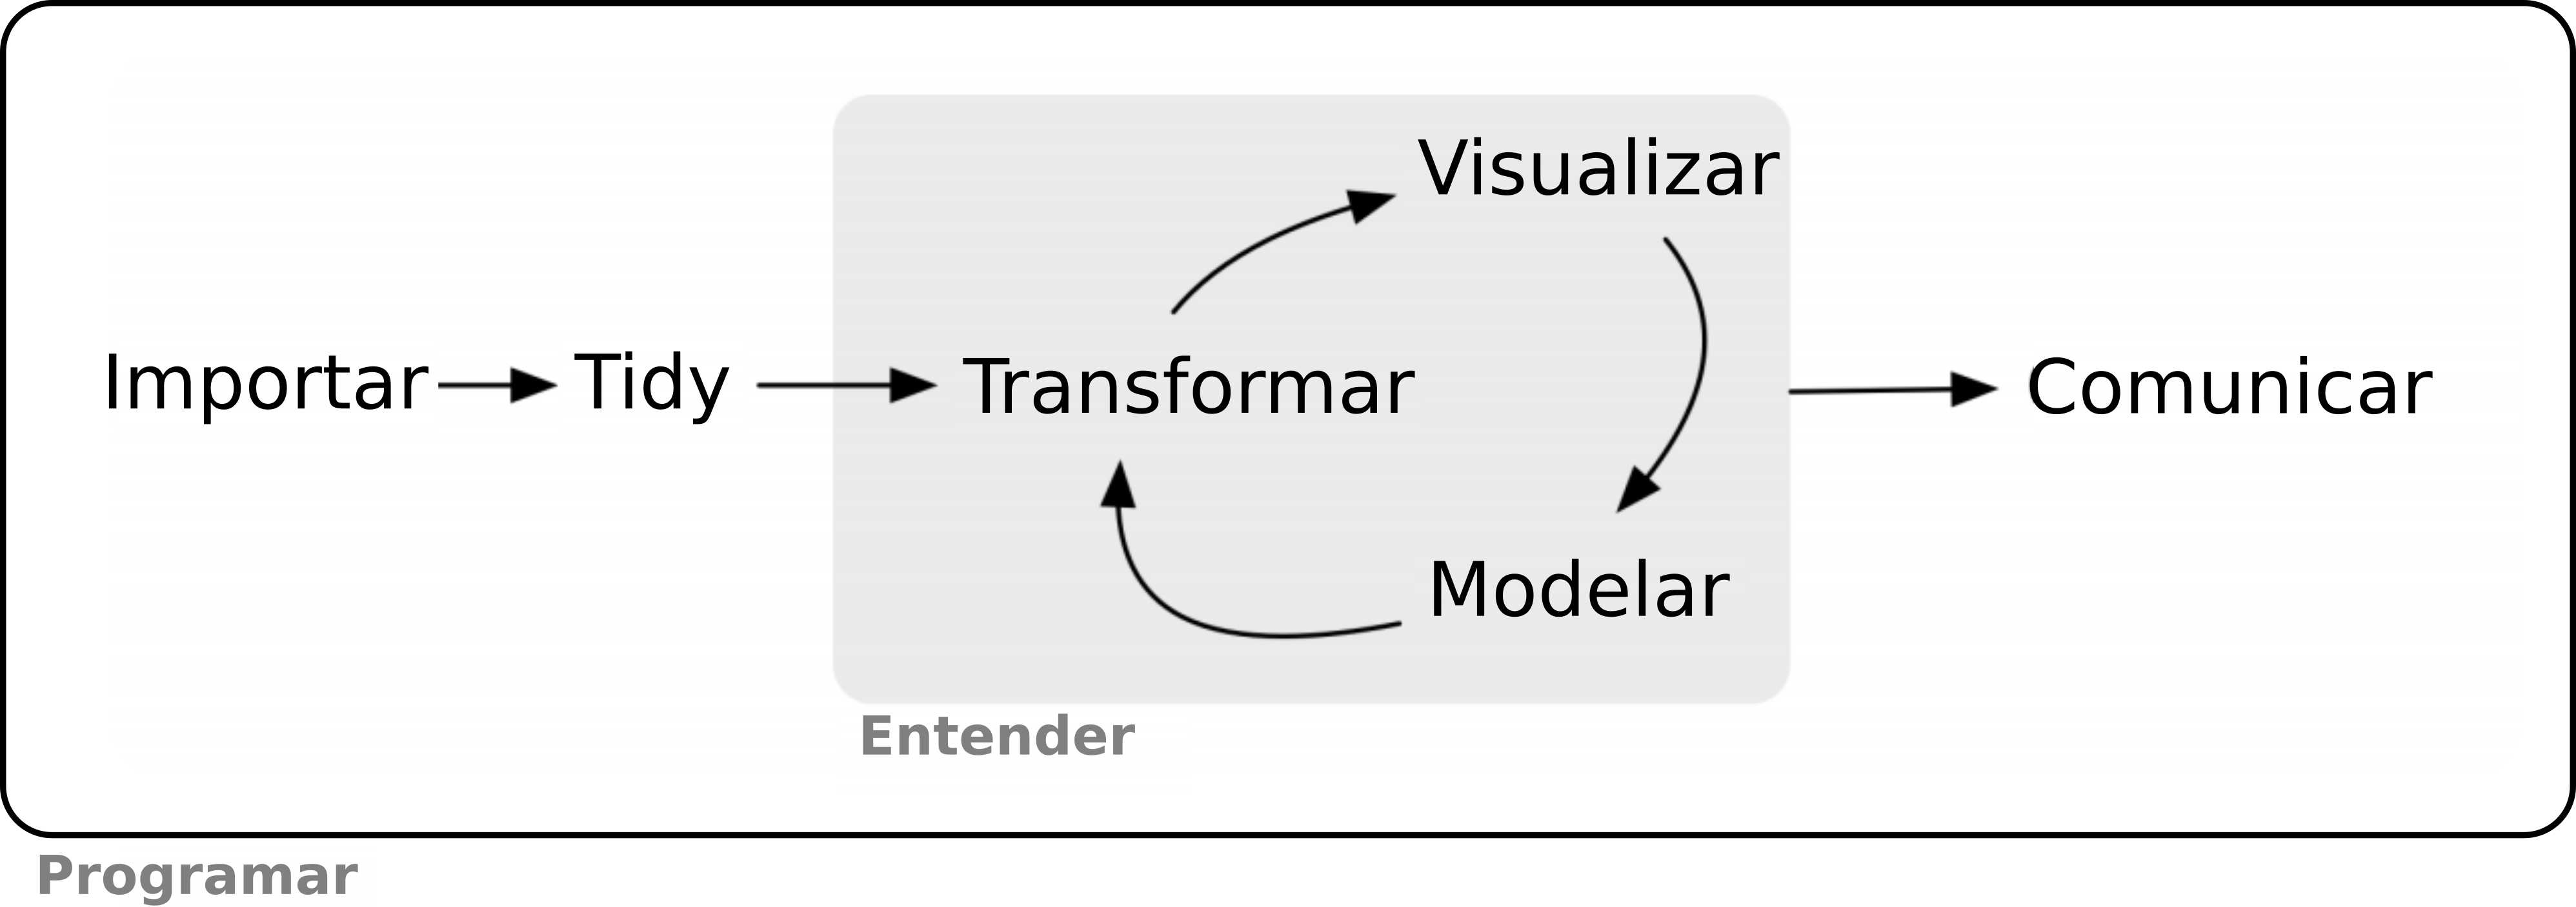
\includegraphics[width=0.7\linewidth]{img/cap05_fig01} 

}

\caption{Modelo das ferramentas necessárias em um projeto típico de ciência de dados: importar, organizar, entender (transformar, visualizar, modelar) e comunicar, envolto à essas ferramentas está a programação. Adaptado de: @wickham2017.}\label{fig:fig-r-tidyverse}
\end{figure}

\hypertarget{tidyverse}{%
\section{\texorpdfstring{\emph{tidyverse}}{tidyverse}}\label{tidyverse}}

Uma vez instalado e carregado, o pacote \texttt{tidyverse} disponibiliza um conjunto de ferramentas através de vários pacotes. Esses pacotes compartilham uma filosofia de design, gramática e estruturas. Podemos entender o \emph{tidyverse} como um ``dialeto novo'' para a linguagem R, onde \emph{tidy} quer dizer organizado, arrumado, ordenado, e \emph{verse} é universo. A seguir, listamos os principais pacotes e suas especificações.

\begin{itemize}
\tightlist
\item
  \href{https://readr.tidyverse.org/}{\texttt{readr}}: importa dados tabulares (e.g.~\texttt{.csv} e \texttt{.txt})
\item
  \href{https://tibble.tidyverse.org/}{\texttt{tibble}}: implementa a classe \texttt{tibble}
\item
  \href{https://tidyr.tidyverse.org/}{\texttt{tidyr}}: transformação de dados para \texttt{tidy}
\item
  \href{https://dplyr.tidyverse.org/}{\texttt{dplyr}}: manipulação de dados
\item
  \href{https://github.com/tidyverse/stringr}{\texttt{stringr}}: manipulação de caracteres
\item
  \href{https://github.com/hadley/forcats}{\texttt{forcats}}: manipulação de fatores
\item
  \href{https://ggplot2.tidyverse.org/}{\texttt{ggplot2}}: possibilita a visualização de dados
\item
  \href{https://purrr.tidyverse.org/}{\texttt{purrr}}: disponibiliza ferramentas para programação funcional
\end{itemize}

Além dos pacotes principais, fazemos também menção a outros pacotes que estão dentro dessa abordagem e que trataremos ainda neste capítulo, em outro momento do livro, ou que você leitor(a) deve se familiarizar. Alguns pacotes compõem o tidyverse outros são mais gerais, entretanto, todos estão envolvidos de alguma forma com Data Science.

\begin{itemize}
\tightlist
\item
  \href{https://readxl.tidyverse.org/}{\texttt{readxl}} e \href{https://cran.r-project.org/package=writexl}{\texttt{writexl}}: importa e exporta dados tabulares (.xlsx)
\item
  \href{http://sfirke.github.io/janitor/}{\texttt{janitor}}: examinar e limpar dados sujos
\item
  \href{https://github.com/rstats-db/DBI}{\texttt{DBI}}: interface de banco de dados R
\item
  \href{https://github.com/tidyverse/haven}{\texttt{haven}}: importa e exporta dados do SPSS, Stata e SAS
\item
  \href{https://github.com/r-lib/httr}{\texttt{httr}}: ferramentas para trabalhar com URLs e HTTP
\item
  \href{https://github.com/tidyverse/rvest}{\texttt{rvest}}: coletar facilmente (raspe) páginas da web
\item
  \href{https://github.com/r-lib/xml2}{\texttt{xml2}}: trabalhar com arquivos XML
\item
  \href{https://github.com/jeroen/jsonlite}{\texttt{jsonlite}}: um analisador e gerador JSON simples e robusto para R
\item
  \href{https://github.com/rstats-db/hms}{\texttt{hms}}: hora do dia
\item
  \href{https://github.com/tidyverse/lubridate}{\texttt{lubridate}}: facilita o tratamento de datas
\item
  \href{https://magrittr.tidyverse.org/}{\texttt{magrittr}}: provê os operadores pipe (\texttt{\%\textgreater{}\%}, \texttt{\%\$\%}, \texttt{\%\textless{}\textgreater{}\%})
\item
  \href{https://github.com/tidyverse/glue}{\texttt{glue}}: facilita combinar dados e caracteres
\item
  \href{https://rmarkdown.rstudio.com/}{\texttt{rmarkdown}}: cria documentos de análise dinâmica que combinam código, saída renderizada (como figuras) e texto
\item
  \href{https://yihui.org/knitr/}{\texttt{knitr}}: projetado para ser um mecanismo transparente para geração de relatórios dinâmicos com R
\item
  \href{https://shiny.rstudio.com/}{\texttt{shiny}}: framework de aplicativo Web para R
\item
  \href{https://rmarkdown.rstudio.com/flexdashboard/}{\texttt{flexdashboard}}: painéis interativos para R
\item
  \href{https://here.r-lib.org/}{\texttt{here}}: facilita a definição de diretórios
\item
  \href{https://usethis.r-lib.org/}{\texttt{usethis}}: automatiza tarefas durante a configuração e desenvolvimento de projetos (Git, `GitHub' e Projetos RStudio)
\item
  \href{https://rdatatable.gitlab.io/data.table/}{\texttt{data.table}}: pacote que fornece uma versão de alto desempenho do \texttt{data.frame} (importar, manipular e expotar)
\item
  \href{https://rstudio.github.io/reticulate/}{\texttt{reticulate}}: pacote que fornece ferramentas para integrar Python e R
\item
  \href{https://spark.rstudio.com/}{\texttt{sparklyr}}: interface R para Apache Spark
\item
  \href{https://github.com/tidymodels/broom}{\texttt{broom}}: converte objetos estatísticos em tibbles organizados
\item
  \href{https://github.com/tidyverse/modelr}{\texttt{modelr}}: funções de modelagem que funcionam com o pipe
\item
  \href{https://www.tidymodels.org/}{\texttt{tidymodels}}: coleção de pacotes para modelagem e aprendizado de máquina usando os princípios do tidyverse
\end{itemize}

Destacamos a grande expansão e aplicabilidade dos pacotes \href{https://rmarkdown.rstudio.com/}{rmarkdown}, \href{https://yihui.org/knitr/}{knitr} e \href{https://bookdown.org/}{bookdown}, que permitiram a escrita desse livro usando essas ferramentas.

Para instalar os principais pacotes que integram o \emph{tidyverse} podemos instalar o pacote \texttt{tidyverse}.

\begin{Shaded}
\begin{Highlighting}[]
\DocumentationTok{\#\# Instalar o pacote tidyverse}
\FunctionTok{install.packages}\NormalTok{(}\StringTok{"tidyverse"}\NormalTok{)}
\end{Highlighting}
\end{Shaded}

Quando carregamos o pacote \texttt{tidyverse} podemos notar uma mensagem indicando quais pacotes foram carregados, suas respectivas versões e os conflitos com outros pacotes.

\begin{Shaded}
\begin{Highlighting}[]
\DocumentationTok{\#\# Carregar o pacote tidyverse}
\FunctionTok{library}\NormalTok{(tidyverse)}
\end{Highlighting}
\end{Shaded}

Podemos ainda listar todos os pacotes do \emph{tidyverse} com a função \texttt{tidyverse::tidyverse\_packages()}.

\begin{Shaded}
\begin{Highlighting}[]
\DocumentationTok{\#\# Listar todos os pacotes do tidyverse }
\NormalTok{tidyverse}\SpecialCharTok{::}\FunctionTok{tidyverse\_packages}\NormalTok{()}
\CommentTok{\#\textgreater{}  [1] "broom"         "cli"           "crayon"        "dbplyr"       }
\CommentTok{\#\textgreater{}  [5] "dplyr"         "dtplyr"        "forcats"       "googledrive"  }
\CommentTok{\#\textgreater{}  [9] "googlesheets4" "ggplot2"       "haven"         "hms"          }
\CommentTok{\#\textgreater{} [13] "httr"          "jsonlite"      "lubridate"     "magrittr"     }
\CommentTok{\#\textgreater{} [17] "modelr"        "pillar"        "purrr"         "readr"        }
\CommentTok{\#\textgreater{} [21] "readxl"        "reprex"        "rlang"         "rstudioapi"   }
\CommentTok{\#\textgreater{} [25] "rvest"         "stringr"       "tibble"        "tidyr"        }
\CommentTok{\#\textgreater{} [29] "xml2"          "tidyverse"}
\end{Highlighting}
\end{Shaded}

Também podemos verificar se os pacotes estão atualizados, senão, podemos atualizá-los com a função \texttt{tidyverse::tidyverse\_update()}.

\begin{Shaded}
\begin{Highlighting}[]
\DocumentationTok{\#\# Verificar e atualizar os pacotes do tidyverse }
\NormalTok{tidyverse}\SpecialCharTok{::}\FunctionTok{tidyverse\_update}\NormalTok{(}\AttributeTok{repos =} \StringTok{"http://cran.us.r{-}project.org"}\NormalTok{)}
\CommentTok{\#\textgreater{} The following packages are out of date:}
\CommentTok{\#\textgreater{} }
\CommentTok{\#\textgreater{} * dplyr         (1.0.5 {-}\textgreater{} 1.0.7)}
\CommentTok{\#\textgreater{} * googlesheets4 (0 {-}\textgreater{} 1.0.0)}
\CommentTok{\#\textgreater{} * haven         (2.3.1 {-}\textgreater{} 2.4.3)}
\CommentTok{\#\textgreater{} * readr         (1.4.0 {-}\textgreater{} 2.0.1)}
\CommentTok{\#\textgreater{} * rlang         (0.4.10 {-}\textgreater{} 0.4.11)}
\CommentTok{\#\textgreater{} * tibble        (3.1.0 {-}\textgreater{} 3.1.3)}
\CommentTok{\#\textgreater{} }
\CommentTok{\#\textgreater{} Start a clean R session then run:}
\CommentTok{\#\textgreater{} install.packages(c("dplyr", "googlesheets4", "haven", "readr", "rlang", "tibble"}
\CommentTok{\#\textgreater{} ))}
\end{Highlighting}
\end{Shaded}

Apesar de podermos fazer a instalação e carregamento de todos os pacotes juntos, usando o pacote \texttt{tidyverse}, podemos instalar e carregar os pacotes individualmente.

\begin{Shaded}
\begin{Highlighting}[]
\DocumentationTok{\#\# Instalar os pacotes do tidyverse individualmente}
\FunctionTok{install.packages}\NormalTok{(}\FunctionTok{c}\NormalTok{(}\StringTok{"ggplot2"}\NormalTok{, }\StringTok{"purrr"}\NormalTok{, }\StringTok{"tibble"}\NormalTok{, }\StringTok{"dplyr"}\NormalTok{, }\StringTok{"tidyr"}\NormalTok{, }\StringTok{"stringr"}\NormalTok{, }
                   \StringTok{"readr"}\NormalTok{, }\StringTok{"forcats"}\NormalTok{), }\AttributeTok{dependencies =} \ConstantTok{TRUE}\NormalTok{)}

\DocumentationTok{\#\# Carregar os pacotes do tidyverse individualmente}
\FunctionTok{library}\NormalTok{(ggplot2)}
\FunctionTok{library}\NormalTok{(purrr)}
\FunctionTok{library}\NormalTok{(tibble)}
\FunctionTok{library}\NormalTok{(dplyr)}
\FunctionTok{library}\NormalTok{(tidyr)}
\FunctionTok{library}\NormalTok{(stringr)}
\FunctionTok{library}\NormalTok{(readr)}
\FunctionTok{library}\NormalTok{(forcats)}
\end{Highlighting}
\end{Shaded}

Todas as funções dos pacotes tidyverse usam \textbf{fonte minúscula} e \textbf{\texttt{\_} (\emph{underscore})} para separar os nomes internos das funções, seguindo a mesma sintaxe do python (``Snake Case''). Neste sentido de padronização, é importante destacar ainda que existe um guia próprio para que os scripts sigam a recomendação de padronização, o \href{https://style.tidyverse.org/}{The tidyverse style guide}, criado pelo Hadley Wickham. Para pessoas que desenvolvem existe o \href{https://design.tidyverse.org/}{Tidyverse design guide} criado pelo \emph{Tidyverse team}.

\begin{Shaded}
\begin{Highlighting}[]
\DocumentationTok{\#\# Funções no formato snake case}
\FunctionTok{read\_csv}\NormalTok{()}
\FunctionTok{read\_xlsx}\NormalTok{()}
\FunctionTok{as\_tibble}\NormalTok{()}
\FunctionTok{left\_join}\NormalTok{()}
\FunctionTok{group\_by}\NormalTok{()}
\end{Highlighting}
\end{Shaded}

Por fim, para evitar possíveis conflitos de funções com o mesmo nome entre pacotes, recomendamos fortemente o hábito de usar as funções precedidas do operador \texttt{::} e o respectivo pacote. Assim, garante-se que a função utilizada é referente ao pacote daquela função. Segue um exemplo com as funções apresentadas anteriormente.

\begin{Shaded}
\begin{Highlighting}[]
\DocumentationTok{\#\# Funções seguidas de seus respectivos pacotes}
\NormalTok{readr}\SpecialCharTok{::}\FunctionTok{read\_csv}\NormalTok{()}
\NormalTok{readxl}\SpecialCharTok{::}\FunctionTok{read\_xlsx}\NormalTok{()}
\NormalTok{tibble}\SpecialCharTok{::}\FunctionTok{as\_tibble}\NormalTok{()}
\NormalTok{dplyr}\SpecialCharTok{::}\FunctionTok{left\_join}\NormalTok{()}
\NormalTok{dplyr}\SpecialCharTok{::}\FunctionTok{group\_by}\NormalTok{()}
\end{Highlighting}
\end{Shaded}

Seguindo essas ideias do novo paradigma da \textbf{Ciência de Dados}, outro conjunto de pacotes foi desenvolvido, chamado de \href{https://www.tidymodels.org/}{\texttt{tidymodels}} que atuam no workflow da análise de dados em ciência de dados: separação e reamostragem, pré-processamento, ajuste de modelos e métricas de performasse de ajustes. Por razões de espaço e especificidade, não entraremos em detalhes desse pacote.

Seguindo o workflow da Figura \ref{fig:fig-r-tidyverse}, iremos ver nos itens das próximas seções como esses passos são realizados com funções de cada pacote.

\hypertarget{here}{%
\section{here}\label{here}}

Dentro do workflow do tidyverse, devemos sempre trabalhar com \textbf{Projetos do RStudio}. Junto com o projeto, também podemos fazer uso do pacote \texttt{here}. Ele permite construir caminhos para os arquivos do projeto de forma mais simples e com maior reprodutibilidade.

Esse pacote cobre o ponto que discutimos no capítulo \ref{cap4}, dado que muitas vezes mudar o diretório com a função \texttt{setwd()} tende a ser demorado, principalmente quando se trata de um script em que várias pessoas estão trabalhando em diferentes computadores e sistemas operacionais. Além disso, ele elimina a questão da fragilidade dos scripts, pois geralmente um script está com os diretórios conectados exatamente a um lugar e a um momento. Por fim, ele também simplifica o trabalho com subdiretórios, facilitando importar ou exportar arquivos para subpastas.

Seu uso é relativamente simples: uma vez criado e aberto o RStudio pelo Projeto do RStudio, o diretório automaticamente é definido para o diretório do projeto. Depois disso, podemos usar a função \texttt{here::here()} para definir os subdiretórios onde estão os dados. O exemplo da aplicação fica para a seção seguinte, quando iremos de fato importar um arquivo para o R. Logo abaixo, mostramos como instalar e carregar o pacote \texttt{here}.

\begin{Shaded}
\begin{Highlighting}[]
\DocumentationTok{\#\# Instalar}
\FunctionTok{install.packages}\NormalTok{(}\StringTok{"here"}\NormalTok{)}

\DocumentationTok{\#\# Carregar}
\FunctionTok{library}\NormalTok{(here)}
\end{Highlighting}
\end{Shaded}

\hypertarget{readr-readxl-e-writexl}{%
\section{readr, readxl e writexl}\label{readr-readxl-e-writexl}}

Dado que possuímos um conjunto de dados e que geralmente esse conjunto de dados estará no formato tabular com umas das extensões: .csv, .txt ou .xlsx, usaremos o pacote \texttt{readr} ou \texttt{readxl} para importar esses dados para o R. Esses pacotes leem e escrevem grandes arquivos de forma mais rápida, além de fornecerem medidores de progresso de importação e exportação, e imprimir a informação dos modos das colunas quando faz a importação. Outro ponto bastante positivo é que também classificam automaticamente o modo dos dados de cada coluna, i.e., se uma coluna possui dados numéricos ou apenas texto, essa informação será considerada para classificar o modo da coluna toda. A classe do objeto atribuído quando lido por esses pacotes é automaticamente um \texttt{tibble}, que veremos melhor na seção seguinte. Todas as funções deste pacote são listadas na \href{https://readr.tidyverse.org/reference/index.html}{página de referência} do pacote.

Usamos as funções \texttt{readr::read\_csv()} e \texttt{readr::write\_csv()} para importar e exportar arquivos .csv do R, respectivamente. Para dados com a extensão .txt, podemos utilizar as funções \texttt{readr::read\_tsv()} ou ainda \texttt{readr::read\_delim()}. Para arquivos tabulares com a extensão .xlsx, temos de instalar e carregar dois pacotes adicionais: \texttt{readxl} e \texttt{writexl}, dos quais usaremos as funções \texttt{readxl::read\_excel()}, \texttt{readxl::read\_xlsx()} ou \texttt{readxl::read\_xls()} para importar dados, atentado para o fato de podermos indicar a aba com os dados com o argumento \texttt{sheet}, e \texttt{writexl::write\_xlsx()} para exportar.

\begin{Shaded}
\begin{Highlighting}[]
\DocumentationTok{\#\# Instalar}
\FunctionTok{install.packages}\NormalTok{(}\StringTok{"writexl"}\NormalTok{)}

\DocumentationTok{\#\# Carregar}
\FunctionTok{library}\NormalTok{(readxl)}
\FunctionTok{library}\NormalTok{(writexl)}
\end{Highlighting}
\end{Shaded}

Se o arquivo .csv foi criado com separador de decimais sendo \texttt{.} e separador de colunas sendo \texttt{,}, usamos as funções normalmente. Caso seja criado com separador de decimais sendo \texttt{,} e separador de colunas sendo \texttt{;}, usaríamos a função \texttt{readr::read\_csv2()} para importar e \texttt{readr::write\_csv2()} para exportar nesse formato, que é mais comum no Brasil.

Para exemplificar como essas funções funcionam, vamos importar novamente os dados de comunidades de anfíbios da Mata Atlântica (Atlantic Amphibians, \citet{vancine2018}), que fizemos o download no Capítulo \ref{cap4}. Estamos usando a função \texttt{readr::read\_csv()}, indicando os diretórios com a função \texttt{here::here()}, e a classe do arquivo é \texttt{tibble}. Devemos atentar para o argumento \texttt{locale\ =\ readr::locale(encoding\ =\ "latin1"}, que selecionamos aqui como \texttt{latin1} para corrigir um erro do autor dos dados que publicou esse data paper com erros\ldots{}

\begin{Shaded}
\begin{Highlighting}[]
\DocumentationTok{\#\# Importar locais}
\NormalTok{tidy\_anfibios\_locais }\OtherTok{\textless{}{-}}\NormalTok{ readr}\SpecialCharTok{::}\FunctionTok{read\_csv}\NormalTok{(}
\NormalTok{  here}\SpecialCharTok{::}\FunctionTok{here}\NormalTok{(}\StringTok{"dados"}\NormalTok{, }\StringTok{"tabelas"}\NormalTok{, }\StringTok{"ATLANTIC\_AMPHIBIANS\_sites.csv"}\NormalTok{),}
  \AttributeTok{locale =}\NormalTok{ readr}\SpecialCharTok{::}\FunctionTok{locale}\NormalTok{(}\AttributeTok{encoding =} \StringTok{"latin1"}\NormalTok{)}
\NormalTok{  )}
\CommentTok{\#\textgreater{} }
\CommentTok{\#\textgreater{} {-}{-} Column specification {-}{-}{-}{-}{-}{-}{-}{-}{-}{-}{-}{-}{-}{-}{-}{-}{-}{-}{-}{-}{-}{-}{-}{-}{-}{-}{-}{-}{-}{-}{-}{-}{-}{-}{-}{-}{-}{-}{-}{-}{-}{-}{-}{-}{-}{-}{-}{-}{-}{-}{-}{-}{-}{-}{-}{-}}
\CommentTok{\#\textgreater{} cols(}
\CommentTok{\#\textgreater{}   .default = col\_character(),}
\CommentTok{\#\textgreater{}   reference\_number = col\_double(),}
\CommentTok{\#\textgreater{}   species\_number = col\_double(),}
\CommentTok{\#\textgreater{}   month\_start = col\_double(),}
\CommentTok{\#\textgreater{}   year\_start = col\_double(),}
\CommentTok{\#\textgreater{}   month\_finish = col\_double(),}
\CommentTok{\#\textgreater{}   year\_finish = col\_double(),}
\CommentTok{\#\textgreater{}   effort\_months = col\_double(),}
\CommentTok{\#\textgreater{}   latitude = col\_double(),}
\CommentTok{\#\textgreater{}   longitude = col\_double(),}
\CommentTok{\#\textgreater{}   altitude = col\_double(),}
\CommentTok{\#\textgreater{}   temperature = col\_double(),}
\CommentTok{\#\textgreater{}   precipitation = col\_double()}
\CommentTok{\#\textgreater{} )}
\CommentTok{\#\textgreater{} i Use \textasciigrave{}spec()\textasciigrave{} for the full column specifications.}
\end{Highlighting}
\end{Shaded}

Caso o download não funcione ou haja problemas com a importação, disponibilizamos os dados também no pacote \texttt{ecodados}.

\begin{Shaded}
\begin{Highlighting}[]
\DocumentationTok{\#\# Importar os dados pelo pacote ecodados}
\FunctionTok{data}\NormalTok{(tidy\_anfibios\_locais)}
\FunctionTok{head}\NormalTok{(tidy\_anfibios\_locais)}
\end{Highlighting}
\end{Shaded}

Para se aprofundar no tema, recomendamos a leitura do Capítulo \href{https://r4ds.had.co.nz/data-import.html}{11 Data import} de \citet{wickham2017}.

\hypertarget{tibble}{%
\section{tibble}\label{tibble}}

O \texttt{tibble} (\texttt{tbl\_sf}) é uma versão aprimorada do data frame (\texttt{data.frame}). Ele é a classe aconselhada para que as funções do tidyverse funcionem melhor sobre conjuntos de dados tabulares importados para o R.

Geralmente, quando utilizamos funções tidyverse para importar dados para o R, é essa classe que os dados adquirem depois de importados. Além da importação de dados, podemos criar um tibble no R usando a função \texttt{tibble::tibble()}, semelhante ao uso da função \texttt{data.frame()}. Podemos ainda converter um \texttt{data.frame} para um \texttt{tibble} usando a função \texttt{tibble::as\_tibble()}. Entretanto, em alguns momentos precisaremos da classe \texttt{data.frame} para algumas funções específicas, e podemos converter um \texttt{tibble} para \texttt{data.frame} usando a função \texttt{tibble::as\_data\_frame()}.

Existem duas diferenças principais no uso do \texttt{tibble} e do \texttt{data.frame}: impressão e subconjunto. Objetos da classe \texttt{tibbles} possuem um método de impressão que mostra a contagem do número de linhas e colunas, e apenas as primeiras 10 linhas e todas as colunas que cabem na tela no console, além dos modos ou tipos das colunas. Dessa forma, cada coluna ou variável, pode ser do modo numbers (\texttt{int} ou \texttt{dbl}), character (\texttt{chr}), logical (\texttt{lgl}), factor (\texttt{fctr}), date + time (\texttt{dttm}) e date (\texttt{date}), além de outras \href{https://tibble.tidyverse.org/articles/types.html}{inúmeras possibilidades}.

Todas as funções deste pacote são listadas na \href{https://tibble.tidyverse.org/reference/index.html}{página de referência} do pacote.

\begin{Shaded}
\begin{Highlighting}[]
\DocumentationTok{\#\# Tibble {-} impressão}
\NormalTok{tidy\_anfibios\_locais}
\CommentTok{\#\textgreater{} \# A tibble: 1,163 x 25}
\CommentTok{\#\textgreater{}   id      reference\_number species\_number record sampled\_habitat active\_methods}
\CommentTok{\#\textgreater{}   \textless{}chr\textgreater{}              \textless{}dbl\textgreater{}          \textless{}dbl\textgreater{} \textless{}chr\textgreater{}  \textless{}chr\textgreater{}           \textless{}chr\textgreater{}         }
\CommentTok{\#\textgreater{} 1 amp1001             1001             19 ab     fo,ll           as            }
\CommentTok{\#\textgreater{} 2 amp1002             1002             16 co     fo,la,ll        as            }
\CommentTok{\#\textgreater{} 3 amp1003             1002             14 co     fo,la,ll        as            }
\CommentTok{\#\textgreater{} 4 amp1004             1002             13 co     fo,la,ll        as            }
\CommentTok{\#\textgreater{} 5 amp1005             1003             30 co     fo,ll,br        as            }
\CommentTok{\#\textgreater{} 6 amp1006             1004             42 co     tp,pp,la,ll,is  NA            }
\CommentTok{\#\textgreater{} \# ... with 1,157 more rows, and 19 more variables: passive\_methods \textless{}chr\textgreater{},}
\CommentTok{\#\textgreater{} \#   complementary\_methods \textless{}chr\textgreater{}, period \textless{}chr\textgreater{}, month\_start \textless{}dbl\textgreater{},}
\CommentTok{\#\textgreater{} \#   year\_start \textless{}dbl\textgreater{}, month\_finish \textless{}dbl\textgreater{}, year\_finish \textless{}dbl\textgreater{},}
\CommentTok{\#\textgreater{} \#   effort\_months \textless{}dbl\textgreater{}, country \textless{}chr\textgreater{}, state \textless{}chr\textgreater{}, state\_abbreviation \textless{}chr\textgreater{},}
\CommentTok{\#\textgreater{} \#   municipality \textless{}chr\textgreater{}, site \textless{}chr\textgreater{}, latitude \textless{}dbl\textgreater{}, longitude \textless{}dbl\textgreater{},}
\CommentTok{\#\textgreater{} \#   coordinate\_precision \textless{}chr\textgreater{}, altitude \textless{}dbl\textgreater{}, temperature \textless{}dbl\textgreater{},}
\CommentTok{\#\textgreater{} \#   precipitation \textless{}dbl\textgreater{}}
\end{Highlighting}
\end{Shaded}

Para o subconjunto, como vimos anteriormente, para selecionar colunas e linhas de objetos bidimensionais podemos utilizar os operadores \texttt{{[}{]}} ou \texttt{{[}{[}{]}{]}}, associado com números separados por vírgulas ou o nome da coluna entre aspas, e o operador \texttt{\$} para extrair uma coluna pelo seu nome. Comparando um \texttt{data.frame} a um \texttt{tibble}, o último é mais rígido na seleção das colunas: eles nunca fazem correspondência parcial e gerarão um aviso se a coluna que você está tentando acessar não existir.

\begin{Shaded}
\begin{Highlighting}[]
\DocumentationTok{\#\# Tibble {-} subconjunto}
\NormalTok{tidy\_anfibios\_locais}\SpecialCharTok{$}\NormalTok{ref}
\CommentTok{\#\textgreater{} Warning: Unknown or uninitialised column: \textasciigrave{}ref\textasciigrave{}.}
\CommentTok{\#\textgreater{} NULL}
\end{Highlighting}
\end{Shaded}

Por fim, podemos ``espiar'' os dados utilizando a função \texttt{tibble::glimpse()} para ter uma noção geral de número de linhas, colunas, e conteúdo de todas as colunas. Essa é função \emph{tidyverse} da função R Base \texttt{str()}.

\begin{Shaded}
\begin{Highlighting}[]
\DocumentationTok{\#\# Espiar os dados}
\NormalTok{tibble}\SpecialCharTok{::}\FunctionTok{glimpse}\NormalTok{(tidy\_anfibios\_locais[, }\DecValTok{1}\SpecialCharTok{:}\DecValTok{10}\NormalTok{])}
\CommentTok{\#\textgreater{} Rows: 1,163}
\CommentTok{\#\textgreater{} Columns: 10}
\CommentTok{\#\textgreater{} $ id                    \textless{}chr\textgreater{} "amp1001", "amp1002", "amp1003", "amp1004", "amp\textasciitilde{}}
\CommentTok{\#\textgreater{} $ reference\_number      \textless{}dbl\textgreater{} 1001, 1002, 1002, 1002, 1003, 1004, 1005, 1005, \textasciitilde{}}
\CommentTok{\#\textgreater{} $ species\_number        \textless{}dbl\textgreater{} 19, 16, 14, 13, 30, 42, 23, 19, 13, 1, 1, 2, 4, \textasciitilde{}}
\CommentTok{\#\textgreater{} $ record                \textless{}chr\textgreater{} "ab", "co", "co", "co", "co", "co", "co", "co", \textasciitilde{}}
\CommentTok{\#\textgreater{} $ sampled\_habitat       \textless{}chr\textgreater{} "fo,ll", "fo,la,ll", "fo,la,ll", "fo,la,ll", "fo\textasciitilde{}}
\CommentTok{\#\textgreater{} $ active\_methods        \textless{}chr\textgreater{} "as", "as", "as", "as", "as", NA, "as", "as,sb,t\textasciitilde{}}
\CommentTok{\#\textgreater{} $ passive\_methods       \textless{}chr\textgreater{} "pt", "pt", "pt", "pt", NA, NA, NA, NA, "pt", "p\textasciitilde{}}
\CommentTok{\#\textgreater{} $ complementary\_methods \textless{}chr\textgreater{} NA, NA, NA, NA, NA, NA, NA, NA, NA, NA, NA, NA, \textasciitilde{}}
\CommentTok{\#\textgreater{} $ period                \textless{}chr\textgreater{} "mo,da,tw,ni", "mo,da,tw,ni", "mo,da,tw,ni", "mo\textasciitilde{}}
\CommentTok{\#\textgreater{} $ month\_start           \textless{}dbl\textgreater{} 9, 12, 12, 12, 7, NA, 4, 4, 4, 5, 5, 5, 5, 5, 5,\textasciitilde{}}
\end{Highlighting}
\end{Shaded}

Para se aprofundar no tema, recomendamos a leitura do Capítulo \href{https://r4ds.had.co.nz/tibbles.html}{10 Tibbles} de \citet{wickham2017}.

\hypertarget{magrittr-pipe--}{%
\section{magrittr (pipe - \%\textgreater\%)}\label{magrittr-pipe--}}

O operador pipe \texttt{\%\textgreater{}\%} permite o encadeamento de várias funções, eliminando a necessidade de criar objetos para armazenar resultados intermediários. Dessa forma, pipes são uma ferramenta poderosa para expressar uma sequência de múltiplas operações.

O operador pipe \texttt{\%\textgreater{}\%} vem do pacote \texttt{magrittr}, entretanto, todos os pacotes no tidyverse automaticamente tornam o pipe disponível. Essa função torna os códigos em R mais simples, pois realizamos múltiplas operações em uma única linha. Ele captura o resultado de uma declaração e o torna a entrada da próxima declaração, então podemos pensar como ``EM SEGUIDA FAÇA'' ao final de cada linha de código.

Todas as funções deste pacote são listadas na \href{https://maggritr.tidyverse.org/reference/index.html}{página de referência} do pacote.

A principal vantagem do uso dos pipes é facilitar o \textbf{debuging} (achar erros) nos códigos, porque seu uso torna a linguagem R mais próxima do que falamos e pensamos, uma vez que evita o uso de funções dentro de funções (funções compostas, lembra-se do fog e gof? Evitamos eles aqui também\ldots).

Digitar \texttt{\%\textgreater{}\%} é um pouco chato, dessa forma, existe um atalho para sua inserção nos scripts: \texttt{Ctrl\ +\ Shift\ +\ M}.

Para deixar esse tópico menos estranho a quem possa ver essa operação pela primeira vez, vamos fazer alguns exemplos.

\begin{Shaded}
\begin{Highlighting}[]
\DocumentationTok{\#\# Base R {-} sem pipe}
\FunctionTok{sqrt}\NormalTok{(}\FunctionTok{sum}\NormalTok{(}\DecValTok{1}\SpecialCharTok{:}\DecValTok{100}\NormalTok{))}
\CommentTok{\#\textgreater{} [1] 71.06335}

\DocumentationTok{\#\# Tidyverse {-} com pipe}
\DecValTok{1}\SpecialCharTok{:}\DecValTok{100} \SpecialCharTok{\%\textgreater{}\%} 
  \FunctionTok{sum}\NormalTok{() }\SpecialCharTok{\%\textgreater{}\%} 
  \FunctionTok{sqrt}\NormalTok{()}
\CommentTok{\#\textgreater{} [1] 71.06335}
\end{Highlighting}
\end{Shaded}

Essas operações ainda estão simples, vamos torná-las mais complexas com várias funções compostas. É nesses casos que a propriedade organizacional do uso do pipe emerge: podemos facilmente ver o encadeamento de operações, onde cada função é disposta numa linha. Apenas um adendo: a função \texttt{set.seed()} que fixa a amostragem de funções que geram valores aleatório, como é o caso da função \texttt{rpois()}.

\begin{Shaded}
\begin{Highlighting}[]
\DocumentationTok{\#\# Fixar amostragem}
\FunctionTok{set.seed}\NormalTok{(}\DecValTok{42}\NormalTok{)}

\DocumentationTok{\#\# Base R {-} sem pipe}
\NormalTok{ve }\OtherTok{\textless{}{-}} \FunctionTok{sum}\NormalTok{(}\FunctionTok{sqrt}\NormalTok{(}\FunctionTok{sort}\NormalTok{(}\FunctionTok{log10}\NormalTok{(}\FunctionTok{rpois}\NormalTok{(}\DecValTok{100}\NormalTok{, }\DecValTok{10}\NormalTok{)))))}
\NormalTok{ve}
\CommentTok{\#\textgreater{} [1] 99.91426}

\DocumentationTok{\#\# Fixar amostragem}
\FunctionTok{set.seed}\NormalTok{(}\DecValTok{42}\NormalTok{)}

\DocumentationTok{\#\# Tidyverse {-} com pipe}
\NormalTok{ve }\OtherTok{\textless{}{-}} \FunctionTok{rpois}\NormalTok{(}\DecValTok{100}\NormalTok{, }\DecValTok{10}\NormalTok{) }\SpecialCharTok{\%\textgreater{}\%} 
  \FunctionTok{log10}\NormalTok{() }\SpecialCharTok{\%\textgreater{}\%}
  \FunctionTok{sort}\NormalTok{() }\SpecialCharTok{\%\textgreater{}\%} 
  \FunctionTok{sqrt}\NormalTok{() }\SpecialCharTok{\%\textgreater{}\%} 
  \FunctionTok{sum}\NormalTok{()}
\NormalTok{ve}
\CommentTok{\#\textgreater{} [1] 99.91426}
\end{Highlighting}
\end{Shaded}

O uso do pipe vai se tornar especialmente útil quando seguirmos para os pacotes das próximas duas seções: \texttt{tidyr} e \texttt{dplyr}. Com esses pacotes faremos operações em linhas e colunas de nossos dados tabulares, então podemos encadear uma série de funções para manipulação, limpeza e análise de dados.

Há ainda três outras variações do pipe que podem ser úteis em alguns momentos, mas que para funcionar precisam que o pacote\texttt{magrittr} seja carregado:

\begin{itemize}
\tightlist
\item
  \texttt{\%T\textgreater{}\%}: retorna o lado esquerdo em vez do lado direito
\item
  \texttt{\%\$\%}: ``explode'' as variáveis em um quadro de dados
\item
  \texttt{\%\textless{}\textgreater{}\%}: permite atribuição usando pipes
\end{itemize}

Para se aprofundar no tema, recomendamos a leitura do Capítulo \href{https://r4ds.had.co.nz/pipes.html}{18 Pipes} de \citet{wickham2017}.

\textbf{Observação}: A partir da versão do R 4.1+ (18/05/2021), o operador pipe se tornou nativo do R. Entretanto, o operador foi atualizado para \texttt{\textbar{}\textgreater{}}, podendo ser inserido com o mesmo atalho \texttt{Ctrl\ +\ Shift\ +\ M}, mas necessitando uma mudança de opção em \texttt{Tools\ \textgreater{}\ Global\ Options\ \textgreater{}\ Code\ \textgreater{}\ {[}x{]}\ Use\ native\ pipe\ operator,\ \textbar{}\textgreater{}\ (requires\ R\ 4.1+)}, necessitando que o RStudio esteja numa versão igual ou superior a 1.4.17+.

\hypertarget{tidyr}{%
\section{tidyr}\label{tidyr}}

Os conjuntos de dados \texttt{tidy} (organizados) são mais fáceis de manipular, modelar e visualizar. Um conjunto de dados está no formato \texttt{tidy} ou não, dependendo de como linhas, colunas e células são combinadas com observações, variáveis e valores. Nos dados tidy, as variáveis estão nas colunas, observações estão nas linhas e valores estão nas células, sendo que para esse último, não deve haver mais de um valor por célula (Figura \ref{fig:fig-r-dados-tidy}).

\begin{enumerate}
\def\labelenumi{\arabic{enumi}.}
\tightlist
\item
  Cada variável em uma coluna
\item
  Cada observação em uma linha
\item
  Cada valor como uma célula
\end{enumerate}

\begin{figure}

{\centering 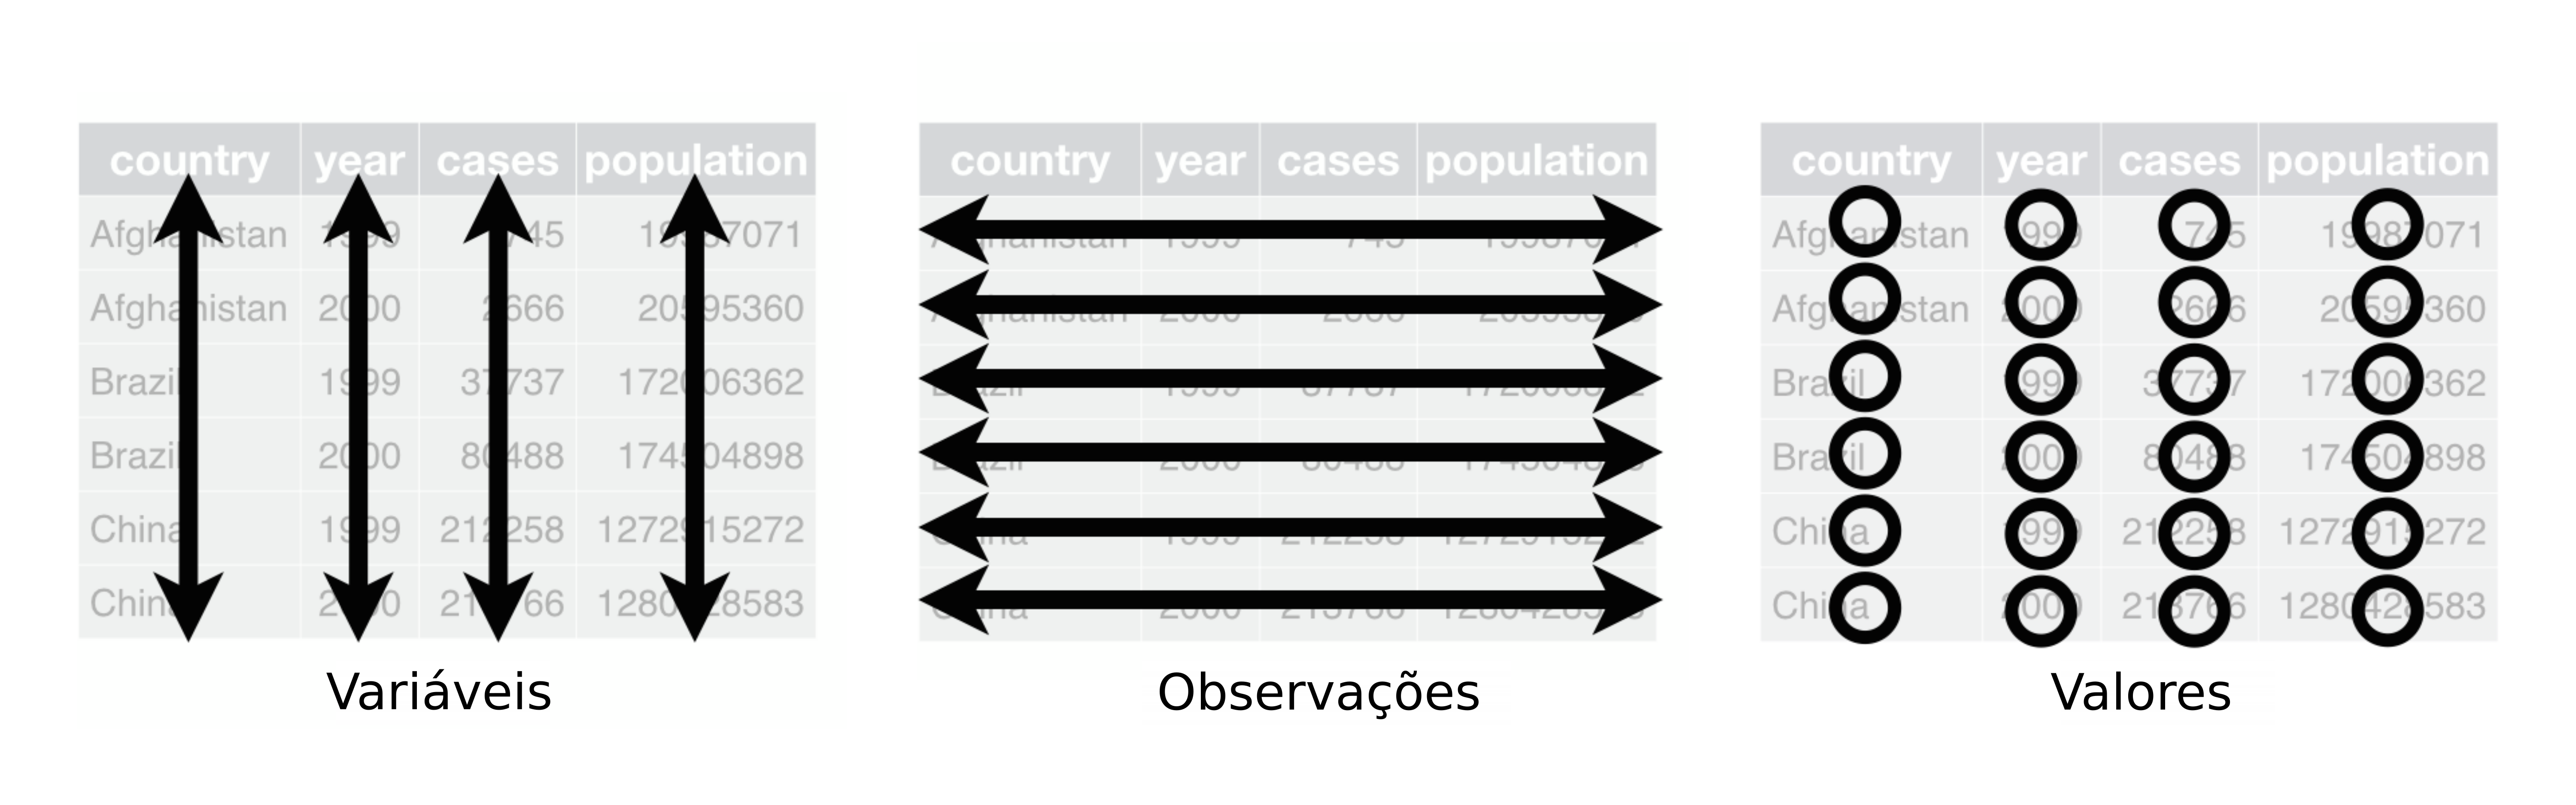
\includegraphics[width=0.7\linewidth]{img/cap05_fig02} 

}

\caption{As três regras que tornam um conjunto de dados *tidy*. Adaptado de: @wickham2017.}\label{fig:fig-r-dados-tidy}
\end{figure}

Todas as funções deste pacote são listadas na \href{https://tidyr.tidyverse.org/reference/index.html}{página de referência} do pacote.

Para realizar diversas transformações nos dados, a fim de ajustá-los ao formato \texttt{tidy} existe uma série de funções, para: unir colunas, separar colunas, lidar com valores faltantes (\texttt{NA}), transformar a base de dados de formato longo para largo (ou vice-e-versa), além de outras \href{https://tidyr.tidyverse.org/reference/index.html}{funções específicas}.

\begin{itemize}
\tightlist
\item
  \texttt{unite()}: junta dados de múltiplas colunas em uma coluna
\item
  \texttt{separate()}: separa caracteres em múltiplas colunas
\item
  \texttt{separate\_rows()}: separa caracteres em múltiplas colunas e linhas
\item
  \texttt{drop\_na()}: retira linhas com \texttt{NA} do conjunto de dados
\item
  \texttt{replace\_na()}: substitui \texttt{NA} do conjunto de dados
\item
  \texttt{pivot\_wider()}: transforma um conjunto de dados longo (\emph{long}) para largo (\emph{wide})
\item
  \texttt{pivot\_longer()}: transforma um conjunto de dados largo (\emph{wide}) para longo (\emph{long})
\end{itemize}

\hypertarget{palmerpenguins}{%
\subsection{palmerpenguins}\label{palmerpenguins}}

Para exemplificar o funcionamento dessas funções, usaremos os dados de medidas de pinguins chamados \href{https://allisonhorst.github.io/palmerpenguins}{\emph{palmerpenguins}}, disponíveis no pacote \texttt{palmerpenguins}.

\begin{Shaded}
\begin{Highlighting}[]
\DocumentationTok{\#\# Instalar o pacote}
\FunctionTok{install.packages}\NormalTok{(}\StringTok{"palmerpenguins"}\NormalTok{)}
\end{Highlighting}
\end{Shaded}

Esses dados foram coletados e disponibilizados pela \href{https://www.uaf.edu/cfos/people/faculty/detail/kristen-gorman.php}{Dra. Kristen Gorman} e pela \href{https://pal.lternet.edu/}{Palmer Station, Antarctica LTER}, membro da Long Term Ecological Research Network.

O pacote \texttt{palmerpenguins} contém dois conjuntos de dados. Um é chamado de \texttt{penguins}, e é uma versão simplificada dos dados brutos. O segundo conjunto de dados é \texttt{penguins\_raw} e contém todas as variáveis e nomes originais baixados. Ambos os conjuntos de dados contêm dados para 344 pinguins, de três espécies diferentes, coletados em três ilhas no arquipélago de Palmer, na Antártica. Destacamos também a versão traduzida desses dados para o português, disponível no pacote \href{https://cienciadedatos.github.io/dados/}{\texttt{dados}}.

Vamos utilizar principalmente o conjunto de dados \texttt{penguins\_raw}, que é a versão dos dados brutos.

\begin{Shaded}
\begin{Highlighting}[]
\DocumentationTok{\#\# Carregar o pacote palmerpenguins}
\FunctionTok{library}\NormalTok{(palmerpenguins)}

\DocumentationTok{\#\# Ajuda dos dados}
\NormalTok{?penguins}
\NormalTok{?penguins\_raw}
\end{Highlighting}
\end{Shaded}

\hypertarget{glimpse}{%
\subsection{glimpse()}\label{glimpse}}

Primeiramente, vamos observar os dados e utilizar a função \texttt{tibble::glimpse()} para ter uma noção geral.

\begin{Shaded}
\begin{Highlighting}[]
\DocumentationTok{\#\# Visualizar os dados}
\NormalTok{penguins\_raw}
\CommentTok{\#\textgreater{} \# A tibble: 344 x 17}
\CommentTok{\#\textgreater{}   studyName \textasciigrave{}Sample Number\textasciigrave{} Species       Region Island  Stage   \textasciigrave{}Individual ID\textasciigrave{}}
\CommentTok{\#\textgreater{}   \textless{}chr\textgreater{}               \textless{}dbl\textgreater{} \textless{}chr\textgreater{}         \textless{}chr\textgreater{}  \textless{}chr\textgreater{}   \textless{}chr\textgreater{}   \textless{}chr\textgreater{}          }
\CommentTok{\#\textgreater{} 1 PAL0708                 1 Adelie Pengu\textasciitilde{} Anvers Torger\textasciitilde{} Adult,\textasciitilde{} N1A1           }
\CommentTok{\#\textgreater{} 2 PAL0708                 2 Adelie Pengu\textasciitilde{} Anvers Torger\textasciitilde{} Adult,\textasciitilde{} N1A2           }
\CommentTok{\#\textgreater{} 3 PAL0708                 3 Adelie Pengu\textasciitilde{} Anvers Torger\textasciitilde{} Adult,\textasciitilde{} N2A1           }
\CommentTok{\#\textgreater{} 4 PAL0708                 4 Adelie Pengu\textasciitilde{} Anvers Torger\textasciitilde{} Adult,\textasciitilde{} N2A2           }
\CommentTok{\#\textgreater{} 5 PAL0708                 5 Adelie Pengu\textasciitilde{} Anvers Torger\textasciitilde{} Adult,\textasciitilde{} N3A1           }
\CommentTok{\#\textgreater{} 6 PAL0708                 6 Adelie Pengu\textasciitilde{} Anvers Torger\textasciitilde{} Adult,\textasciitilde{} N3A2           }
\CommentTok{\#\textgreater{} \# ... with 338 more rows, and 10 more variables: Clutch Completion \textless{}chr\textgreater{},}
\CommentTok{\#\textgreater{} \#   Date Egg \textless{}date\textgreater{}, Culmen Length (mm) \textless{}dbl\textgreater{}, Culmen Depth (mm) \textless{}dbl\textgreater{},}
\CommentTok{\#\textgreater{} \#   Flipper Length (mm) \textless{}dbl\textgreater{}, Body Mass (g) \textless{}dbl\textgreater{}, Sex \textless{}chr\textgreater{},}
\CommentTok{\#\textgreater{} \#   Delta 15 N (o/oo) \textless{}dbl\textgreater{}, Delta 13 C (o/oo) \textless{}dbl\textgreater{}, Comments \textless{}chr\textgreater{}}

\DocumentationTok{\#\# Espiar os dados}
\NormalTok{dplyr}\SpecialCharTok{::}\FunctionTok{glimpse}\NormalTok{(penguins\_raw)}
\CommentTok{\#\textgreater{} Rows: 344}
\CommentTok{\#\textgreater{} Columns: 17}
\CommentTok{\#\textgreater{} $ studyName             \textless{}chr\textgreater{} "PAL0708", "PAL0708", "PAL0708", "PAL0708", "PAL\textasciitilde{}}
\CommentTok{\#\textgreater{} $ \textasciigrave{}Sample Number\textasciigrave{}       \textless{}dbl\textgreater{} 1, 2, 3, 4, 5, 6, 7, 8, 9, 10, 11, 12, 13, 14, 1\textasciitilde{}}
\CommentTok{\#\textgreater{} $ Species               \textless{}chr\textgreater{} "Adelie Penguin (Pygoscelis adeliae)", "Adelie P\textasciitilde{}}
\CommentTok{\#\textgreater{} $ Region                \textless{}chr\textgreater{} "Anvers", "Anvers", "Anvers", "Anvers", "Anvers"\textasciitilde{}}
\CommentTok{\#\textgreater{} $ Island                \textless{}chr\textgreater{} "Torgersen", "Torgersen", "Torgersen", "Torgerse\textasciitilde{}}
\CommentTok{\#\textgreater{} $ Stage                 \textless{}chr\textgreater{} "Adult, 1 Egg Stage", "Adult, 1 Egg Stage", "Adu\textasciitilde{}}
\CommentTok{\#\textgreater{} $ \textasciigrave{}Individual ID\textasciigrave{}       \textless{}chr\textgreater{} "N1A1", "N1A2", "N2A1", "N2A2", "N3A1", "N3A2", \textasciitilde{}}
\CommentTok{\#\textgreater{} $ \textasciigrave{}Clutch Completion\textasciigrave{}   \textless{}chr\textgreater{} "Yes", "Yes", "Yes", "Yes", "Yes", "Yes", "No", \textasciitilde{}}
\CommentTok{\#\textgreater{} $ \textasciigrave{}Date Egg\textasciigrave{}            \textless{}date\textgreater{} 2007{-}11{-}11, 2007{-}11{-}11, 2007{-}11{-}16, 2007{-}11{-}16,\textasciitilde{}}
\CommentTok{\#\textgreater{} $ \textasciigrave{}Culmen Length (mm)\textasciigrave{}  \textless{}dbl\textgreater{} 39.1, 39.5, 40.3, NA, 36.7, 39.3, 38.9, 39.2, 34\textasciitilde{}}
\CommentTok{\#\textgreater{} $ \textasciigrave{}Culmen Depth (mm)\textasciigrave{}   \textless{}dbl\textgreater{} 18.7, 17.4, 18.0, NA, 19.3, 20.6, 17.8, 19.6, 18\textasciitilde{}}
\CommentTok{\#\textgreater{} $ \textasciigrave{}Flipper Length (mm)\textasciigrave{} \textless{}dbl\textgreater{} 181, 186, 195, NA, 193, 190, 181, 195, 193, 190,\textasciitilde{}}
\CommentTok{\#\textgreater{} $ \textasciigrave{}Body Mass (g)\textasciigrave{}       \textless{}dbl\textgreater{} 3750, 3800, 3250, NA, 3450, 3650, 3625, 4675, 34\textasciitilde{}}
\CommentTok{\#\textgreater{} $ Sex                   \textless{}chr\textgreater{} "MALE", "FEMALE", "FEMALE", NA, "FEMALE", "MALE"\textasciitilde{}}
\CommentTok{\#\textgreater{} $ \textasciigrave{}Delta 15 N (o/oo)\textasciigrave{}   \textless{}dbl\textgreater{} NA, 8.94956, 8.36821, NA, 8.76651, 8.66496, 9.18\textasciitilde{}}
\CommentTok{\#\textgreater{} $ \textasciigrave{}Delta 13 C (o/oo)\textasciigrave{}   \textless{}dbl\textgreater{} NA, {-}24.69454, {-}25.33302, NA, {-}25.32426, {-}25.298\textasciitilde{}}
\CommentTok{\#\textgreater{} $ Comments              \textless{}chr\textgreater{} "Not enough blood for isotopes.", NA, NA, "Adult\textasciitilde{}}
\end{Highlighting}
\end{Shaded}

\hypertarget{unite}{%
\subsection{unite()}\label{unite}}

Primeiramente, vamos exemplificar como juntar e separar colunas. Vamos utilizar a função \texttt{tidyr::unite()} para unir as colunas. Há diversos parâmetros para alterar como essa função funciona, entretanto, é importante destacar três deles: \texttt{col} nome da coluna que vai receber as colunas unidas, \texttt{sep} indicando o caracter separador das colunas unidas, e \texttt{remove} para uma resposta lógica se as colunas unidas são removidas ou não. Vamos unir as colunas ``Region'' e ``Island'' na nova coluna ``region\_island''.

\begin{Shaded}
\begin{Highlighting}[]
\DocumentationTok{\#\# Unir colunas}
\NormalTok{penguins\_raw\_unir }\OtherTok{\textless{}{-}}\NormalTok{ tidyr}\SpecialCharTok{::}\FunctionTok{unite}\NormalTok{(}\AttributeTok{data =}\NormalTok{ penguins\_raw, }
                                  \AttributeTok{col =} \StringTok{"region\_island"}\NormalTok{,}
\NormalTok{                                  Region}\SpecialCharTok{:}\NormalTok{Island, }
                                  \AttributeTok{sep =} \StringTok{", "}\NormalTok{,}
                                  \AttributeTok{remove =} \ConstantTok{FALSE}\NormalTok{)}
\FunctionTok{head}\NormalTok{(penguins\_raw\_unir[, }\FunctionTok{c}\NormalTok{(}\StringTok{"Region"}\NormalTok{, }\StringTok{"Island"}\NormalTok{, }\StringTok{"region\_island"}\NormalTok{)])}
\CommentTok{\#\textgreater{} \# A tibble: 6 x 3}
\CommentTok{\#\textgreater{}   Region Island    region\_island    }
\CommentTok{\#\textgreater{}   \textless{}chr\textgreater{}  \textless{}chr\textgreater{}     \textless{}chr\textgreater{}            }
\CommentTok{\#\textgreater{} 1 Anvers Torgersen Anvers, Torgersen}
\CommentTok{\#\textgreater{} 2 Anvers Torgersen Anvers, Torgersen}
\CommentTok{\#\textgreater{} 3 Anvers Torgersen Anvers, Torgersen}
\CommentTok{\#\textgreater{} 4 Anvers Torgersen Anvers, Torgersen}
\CommentTok{\#\textgreater{} 5 Anvers Torgersen Anvers, Torgersen}
\CommentTok{\#\textgreater{} 6 Anvers Torgersen Anvers, Torgersen}
\end{Highlighting}
\end{Shaded}

\hypertarget{separate}{%
\subsection{separate()}\label{separate}}

De forma contrária, podemos utilizar as funções \texttt{tidyr::separate()} e \texttt{tidyr::separate\_rows()} para separar elementos de uma coluna em mais colunas. Respectivamente, a primeira função separa uma coluna em novas colunas conforme a separação, e a segunda função separa uma coluna, distribuindo os elementos também nas linhas. Novamente, há diversos parâmetros para mudar o comportamento dessas funções, mas destacaremos aqui quatro deles: \texttt{col} coluna a ser separada, \texttt{into} os nomes das novas colunas, \texttt{sep} indicando o caractere separador das colunas, e \texttt{remove} para uma resposta lógica se as colunas separadas são removidas ou não. Vamos separar a coluna ``Stage'' nas colunas ``stage'' e ``egg\_stage''.

\begin{Shaded}
\begin{Highlighting}[]
\DocumentationTok{\#\# Separar colunas}
\NormalTok{penguins\_raw\_separar }\OtherTok{\textless{}{-}}\NormalTok{ tidyr}\SpecialCharTok{::}\FunctionTok{separate}\NormalTok{(}\AttributeTok{data =}\NormalTok{ penguins\_raw, }
                                        \AttributeTok{col =}\NormalTok{ Stage,}
                                        \AttributeTok{into =} \FunctionTok{c}\NormalTok{(}\StringTok{"stage"}\NormalTok{, }\StringTok{"egg\_stage"}\NormalTok{), }
                                        \AttributeTok{sep =} \StringTok{", "}\NormalTok{,}
                                        \AttributeTok{remove =} \ConstantTok{FALSE}\NormalTok{)}
\FunctionTok{head}\NormalTok{(penguins\_raw\_separar[, }\FunctionTok{c}\NormalTok{(}\StringTok{"Stage"}\NormalTok{, }\StringTok{"stage"}\NormalTok{, }\StringTok{"egg\_stage"}\NormalTok{)])}
\CommentTok{\#\textgreater{} \# A tibble: 6 x 3}
\CommentTok{\#\textgreater{}   Stage              stage egg\_stage  }
\CommentTok{\#\textgreater{}   \textless{}chr\textgreater{}              \textless{}chr\textgreater{} \textless{}chr\textgreater{}      }
\CommentTok{\#\textgreater{} 1 Adult, 1 Egg Stage Adult 1 Egg Stage}
\CommentTok{\#\textgreater{} 2 Adult, 1 Egg Stage Adult 1 Egg Stage}
\CommentTok{\#\textgreater{} 3 Adult, 1 Egg Stage Adult 1 Egg Stage}
\CommentTok{\#\textgreater{} 4 Adult, 1 Egg Stage Adult 1 Egg Stage}
\CommentTok{\#\textgreater{} 5 Adult, 1 Egg Stage Adult 1 Egg Stage}
\CommentTok{\#\textgreater{} 6 Adult, 1 Egg Stage Adult 1 Egg Stage}

\DocumentationTok{\#\# Separar colunas em novas linhas}
\NormalTok{penguins\_raw\_separar\_linhas }\OtherTok{\textless{}{-}}\NormalTok{ tidyr}\SpecialCharTok{::}\FunctionTok{separate\_rows}\NormalTok{(}\AttributeTok{data =}\NormalTok{ penguins\_raw,}
\NormalTok{                                                    Stage,}
                                                    \AttributeTok{sep =} \StringTok{", "}\NormalTok{)}
\FunctionTok{head}\NormalTok{(penguins\_raw\_separar\_linhas[, }\FunctionTok{c}\NormalTok{(}\StringTok{"studyName"}\NormalTok{, }\StringTok{"Sample Number"}\NormalTok{, }\StringTok{"Species"}\NormalTok{, }
                                     \StringTok{"Region"}\NormalTok{, }\StringTok{"Island"}\NormalTok{, }\StringTok{"Stage"}\NormalTok{)])}
\CommentTok{\#\textgreater{} \# A tibble: 6 x 6}
\CommentTok{\#\textgreater{}   studyName \textasciigrave{}Sample Number\textasciigrave{} Species                    Region Island   Stage    }
\CommentTok{\#\textgreater{}   \textless{}chr\textgreater{}               \textless{}dbl\textgreater{} \textless{}chr\textgreater{}                      \textless{}chr\textgreater{}  \textless{}chr\textgreater{}    \textless{}chr\textgreater{}    }
\CommentTok{\#\textgreater{} 1 PAL0708                 1 Adelie Penguin (Pygosceli\textasciitilde{} Anvers Torgers\textasciitilde{} Adult    }
\CommentTok{\#\textgreater{} 2 PAL0708                 1 Adelie Penguin (Pygosceli\textasciitilde{} Anvers Torgers\textasciitilde{} 1 Egg St\textasciitilde{}}
\CommentTok{\#\textgreater{} 3 PAL0708                 2 Adelie Penguin (Pygosceli\textasciitilde{} Anvers Torgers\textasciitilde{} Adult    }
\CommentTok{\#\textgreater{} 4 PAL0708                 2 Adelie Penguin (Pygosceli\textasciitilde{} Anvers Torgers\textasciitilde{} 1 Egg St\textasciitilde{}}
\CommentTok{\#\textgreater{} 5 PAL0708                 3 Adelie Penguin (Pygosceli\textasciitilde{} Anvers Torgers\textasciitilde{} Adult    }
\CommentTok{\#\textgreater{} 6 PAL0708                 3 Adelie Penguin (Pygosceli\textasciitilde{} Anvers Torgers\textasciitilde{} 1 Egg St\textasciitilde{}}
\end{Highlighting}
\end{Shaded}

\hypertarget{drop_na-e-replace_na}{%
\subsection{drop\_na() e replace\_na()}\label{drop_na-e-replace_na}}

\emph{Valores faltantes} (\texttt{NA}) é um tipo especial de elemento que discutimos no Capítulo \ref{cap4}, e são relativamente comuns em conjuntos de dados. Em Base R, vimos algumas formas de lidar com esse tipo de elemento. No formato \texttt{tidyverse}, existem várias formas de lidar com eles, mas aqui focaremos nas funções \texttt{tidyr::drop\_na()} e \texttt{tidyr::replace\_na()}, para retirar linhas e substitui-los, respectivamente.

\begin{Shaded}
\begin{Highlighting}[]
\DocumentationTok{\#\# Remover todas as linhas com NAs}
\NormalTok{penguins\_raw\_todas\_na }\OtherTok{\textless{}{-}}\NormalTok{ tidyr}\SpecialCharTok{::}\FunctionTok{drop\_na}\NormalTok{(}\AttributeTok{data =}\NormalTok{ penguins\_raw)}
\FunctionTok{head}\NormalTok{(penguins\_raw\_todas\_na)}
\CommentTok{\#\textgreater{} \# A tibble: 6 x 17}
\CommentTok{\#\textgreater{}   studyName \textasciigrave{}Sample Number\textasciigrave{} Species       Region Island  Stage   \textasciigrave{}Individual ID\textasciigrave{}}
\CommentTok{\#\textgreater{}   \textless{}chr\textgreater{}               \textless{}dbl\textgreater{} \textless{}chr\textgreater{}         \textless{}chr\textgreater{}  \textless{}chr\textgreater{}   \textless{}chr\textgreater{}   \textless{}chr\textgreater{}          }
\CommentTok{\#\textgreater{} 1 PAL0708                 7 Adelie Pengu\textasciitilde{} Anvers Torger\textasciitilde{} Adult,\textasciitilde{} N4A1           }
\CommentTok{\#\textgreater{} 2 PAL0708                 8 Adelie Pengu\textasciitilde{} Anvers Torger\textasciitilde{} Adult,\textasciitilde{} N4A2           }
\CommentTok{\#\textgreater{} 3 PAL0708                29 Adelie Pengu\textasciitilde{} Anvers Biscoe  Adult,\textasciitilde{} N18A1          }
\CommentTok{\#\textgreater{} 4 PAL0708                30 Adelie Pengu\textasciitilde{} Anvers Biscoe  Adult,\textasciitilde{} N18A2          }
\CommentTok{\#\textgreater{} 5 PAL0708                39 Adelie Pengu\textasciitilde{} Anvers Dream   Adult,\textasciitilde{} N25A1          }
\CommentTok{\#\textgreater{} 6 PAL0809                69 Adelie Pengu\textasciitilde{} Anvers Torger\textasciitilde{} Adult,\textasciitilde{} N32A1          }
\CommentTok{\#\textgreater{} \# ... with 10 more variables: Clutch Completion \textless{}chr\textgreater{}, Date Egg \textless{}date\textgreater{},}
\CommentTok{\#\textgreater{} \#   Culmen Length (mm) \textless{}dbl\textgreater{}, Culmen Depth (mm) \textless{}dbl\textgreater{},}
\CommentTok{\#\textgreater{} \#   Flipper Length (mm) \textless{}dbl\textgreater{}, Body Mass (g) \textless{}dbl\textgreater{}, Sex \textless{}chr\textgreater{},}
\CommentTok{\#\textgreater{} \#   Delta 15 N (o/oo) \textless{}dbl\textgreater{}, Delta 13 C (o/oo) \textless{}dbl\textgreater{}, Comments \textless{}chr\textgreater{}}

\DocumentationTok{\#\# Remover linhas de colunas específicas com NAs}
\NormalTok{penguins\_raw\_colunas\_na }\OtherTok{\textless{}{-}}\NormalTok{ tidyr}\SpecialCharTok{::}\FunctionTok{drop\_na}\NormalTok{(}\AttributeTok{data =}\NormalTok{ penguins\_raw,}
                                          \FunctionTok{any\_of}\NormalTok{(}\StringTok{"Comments"}\NormalTok{))}
\FunctionTok{head}\NormalTok{(penguins\_raw\_colunas\_na[, }\StringTok{"Comments"}\NormalTok{])}
\CommentTok{\#\textgreater{} \# A tibble: 6 x 1}
\CommentTok{\#\textgreater{}   Comments                             }
\CommentTok{\#\textgreater{}   \textless{}chr\textgreater{}                                }
\CommentTok{\#\textgreater{} 1 Not enough blood for isotopes.       }
\CommentTok{\#\textgreater{} 2 Adult not sampled.                   }
\CommentTok{\#\textgreater{} 3 Nest never observed with full clutch.}
\CommentTok{\#\textgreater{} 4 Nest never observed with full clutch.}
\CommentTok{\#\textgreater{} 5 No blood sample obtained.            }
\CommentTok{\#\textgreater{} 6 No blood sample obtained for sexing.}

\DocumentationTok{\#\# Substituir NAs por outro valor}
\NormalTok{penguins\_raw\_subs\_na }\OtherTok{\textless{}{-}}\NormalTok{ tidyr}\SpecialCharTok{::}\FunctionTok{replace\_na}\NormalTok{(}\AttributeTok{data =}\NormalTok{ penguins\_raw,}
                                          \FunctionTok{list}\NormalTok{(}\AttributeTok{Comments =} \StringTok{"Unknown"}\NormalTok{))}
\FunctionTok{head}\NormalTok{(penguins\_raw\_subs\_na[, }\StringTok{"Comments"}\NormalTok{])}
\CommentTok{\#\textgreater{} \# A tibble: 6 x 1}
\CommentTok{\#\textgreater{}   Comments                      }
\CommentTok{\#\textgreater{}   \textless{}chr\textgreater{}                         }
\CommentTok{\#\textgreater{} 1 Not enough blood for isotopes.}
\CommentTok{\#\textgreater{} 2 Unknown                       }
\CommentTok{\#\textgreater{} 3 Unknown                       }
\CommentTok{\#\textgreater{} 4 Adult not sampled.            }
\CommentTok{\#\textgreater{} 5 Unknown                       }
\CommentTok{\#\textgreater{} 6 Unknown}
\end{Highlighting}
\end{Shaded}

\hypertarget{pivot_longer-e-pivot_wider}{%
\subsection{pivot\_longer() e pivot\_wider()}\label{pivot_longer-e-pivot_wider}}

Por fim, trataremos da pivotagem ou remodelagem de dados. Veremos como mudar o formato do nosso conjunto de dados de longo (\emph{long}) para largo (\emph{wide}) e vice-versa. Essa é uma operação semelhante à ``Tabela Dinâmica'' das planilhas eletrônicas. Consiste em usar uma coluna para distribuir seus valores em outras colunas, de modo que os valores dos elementos são preenchidos corretamente, reduzindo assim o número de linhas. Essa operação é bastante comum em Ecologia de Comunidades, quando queremos transformar uma lista de espécies em uma matriz de comunidades, com várias espécies nas colunas. Para realizar essa operação, usarmos a função \texttt{tidyr::pivot\_wider()}. Dos diversos parâmetros que podem compor essa função, dois deles são fundamentais: \texttt{names\_from} que indica a coluna de onde os nomes serão usados e \texttt{values\_from} a coluna com os valores.

\begin{Shaded}
\begin{Highlighting}[]
\DocumentationTok{\#\# Selecionar colunas}
\NormalTok{penguins\_raw\_sel\_col }\OtherTok{\textless{}{-}}\NormalTok{ penguins\_raw[, }\FunctionTok{c}\NormalTok{(}\DecValTok{2}\NormalTok{, }\DecValTok{3}\NormalTok{, }\DecValTok{13}\NormalTok{)]}
\FunctionTok{head}\NormalTok{(penguins\_raw\_sel\_col)}
\CommentTok{\#\textgreater{} \# A tibble: 6 x 3}
\CommentTok{\#\textgreater{}   \textasciigrave{}Sample Number\textasciigrave{} Species                             \textasciigrave{}Body Mass (g)\textasciigrave{}}
\CommentTok{\#\textgreater{}             \textless{}dbl\textgreater{} \textless{}chr\textgreater{}                                         \textless{}dbl\textgreater{}}
\CommentTok{\#\textgreater{} 1               1 Adelie Penguin (Pygoscelis adeliae)            3750}
\CommentTok{\#\textgreater{} 2               2 Adelie Penguin (Pygoscelis adeliae)            3800}
\CommentTok{\#\textgreater{} 3               3 Adelie Penguin (Pygoscelis adeliae)            3250}
\CommentTok{\#\textgreater{} 4               4 Adelie Penguin (Pygoscelis adeliae)              NA}
\CommentTok{\#\textgreater{} 5               5 Adelie Penguin (Pygoscelis adeliae)            3450}
\CommentTok{\#\textgreater{} 6               6 Adelie Penguin (Pygoscelis adeliae)            3650}

\DocumentationTok{\#\# Pivotar para largo}
\NormalTok{penguins\_raw\_pivot\_wider }\OtherTok{\textless{}{-}}\NormalTok{ tidyr}\SpecialCharTok{::}\FunctionTok{pivot\_wider}\NormalTok{(}\AttributeTok{data =}\NormalTok{ penguins\_raw\_sel\_col, }
                                               \AttributeTok{names\_from =}\NormalTok{ Species, }
                                               \AttributeTok{values\_from =} \StringTok{\textasciigrave{}}\AttributeTok{Body Mass (g)}\StringTok{\textasciigrave{}}\NormalTok{)}
\FunctionTok{head}\NormalTok{(penguins\_raw\_pivot\_wider)}
\CommentTok{\#\textgreater{} \# A tibble: 6 x 4}
\CommentTok{\#\textgreater{}   \textasciigrave{}Sample Number\textasciigrave{} \textasciigrave{}Adelie Penguin (Py\textasciitilde{} \textasciigrave{}Gentoo penguin (Py\textasciitilde{} \textasciigrave{}Chinstrap penguin \textasciitilde{}}
\CommentTok{\#\textgreater{}             \textless{}dbl\textgreater{}                \textless{}dbl\textgreater{}                \textless{}dbl\textgreater{}                \textless{}dbl\textgreater{}}
\CommentTok{\#\textgreater{} 1               1                 3750                 4500                 3500}
\CommentTok{\#\textgreater{} 2               2                 3800                 5700                 3900}
\CommentTok{\#\textgreater{} 3               3                 3250                 4450                 3650}
\CommentTok{\#\textgreater{} 4               4                   NA                 5700                 3525}
\CommentTok{\#\textgreater{} 5               5                 3450                 5400                 3725}
\CommentTok{\#\textgreater{} 6               6                 3650                 4550                 3950}
\end{Highlighting}
\end{Shaded}

De modo oposto, podemos partir de um conjunto de dados largo (\emph{wide}), ou seja, com várias colunas, e queremos que essas colunas preencham uma única coluna, e que os valores antes espalhados nessas várias colunas sejam adicionados um embaixo do outro, numa única coluna. Para essa operação, podemos utilizar a função \texttt{tidyr::pivot\_longer()}. Novamente, dos diversos parâmetros que podem compor essa função, três deles são fundamentais: \texttt{cols} indicando as colunas que serão usadas para serem pivotadas, \texttt{names\_to} que indica a coluna de onde os nomes serão usados e \texttt{values\_to} a coluna com os valores.

\begin{Shaded}
\begin{Highlighting}[]
\DocumentationTok{\#\# Selecionar colunas}
\NormalTok{penguins\_raw\_sel\_col }\OtherTok{\textless{}{-}}\NormalTok{ penguins\_raw[, }\FunctionTok{c}\NormalTok{(}\DecValTok{2}\NormalTok{, }\DecValTok{3}\NormalTok{, }\DecValTok{10}\SpecialCharTok{:}\DecValTok{13}\NormalTok{)]}
\FunctionTok{head}\NormalTok{(penguins\_raw\_sel\_col)}
\CommentTok{\#\textgreater{} \# A tibble: 6 x 6}
\CommentTok{\#\textgreater{}   \textasciigrave{}Sample Number\textasciigrave{} Species    \textasciigrave{}Culmen Length (\textasciitilde{} \textasciigrave{}Culmen Depth (\textasciitilde{} \textasciigrave{}Flipper Length\textasciitilde{}}
\CommentTok{\#\textgreater{}             \textless{}dbl\textgreater{} \textless{}chr\textgreater{}                  \textless{}dbl\textgreater{}            \textless{}dbl\textgreater{}            \textless{}dbl\textgreater{}}
\CommentTok{\#\textgreater{} 1               1 Adelie Pe\textasciitilde{}              39.1             18.7              181}
\CommentTok{\#\textgreater{} 2               2 Adelie Pe\textasciitilde{}              39.5             17.4              186}
\CommentTok{\#\textgreater{} 3               3 Adelie Pe\textasciitilde{}              40.3             18                195}
\CommentTok{\#\textgreater{} 4               4 Adelie Pe\textasciitilde{}              NA               NA                 NA}
\CommentTok{\#\textgreater{} 5               5 Adelie Pe\textasciitilde{}              36.7             19.3              193}
\CommentTok{\#\textgreater{} 6               6 Adelie Pe\textasciitilde{}              39.3             20.6              190}
\CommentTok{\#\textgreater{} \# ... with 1 more variable: Body Mass (g) \textless{}dbl\textgreater{}}

\DocumentationTok{\#\# Pivotar para largo}
\NormalTok{penguins\_raw\_pivot\_longer }\OtherTok{\textless{}{-}}\NormalTok{ tidyr}\SpecialCharTok{::}\FunctionTok{pivot\_longer}\NormalTok{(}\AttributeTok{data =}\NormalTok{ penguins\_raw\_sel\_col, }
                                                 \AttributeTok{cols =} \StringTok{\textasciigrave{}}\AttributeTok{Culmen Length (mm)}\StringTok{\textasciigrave{}}\SpecialCharTok{:}\StringTok{\textasciigrave{}}\AttributeTok{Body Mass (g)}\StringTok{\textasciigrave{}}\NormalTok{,}
                                                 \AttributeTok{names\_to =} \StringTok{"medidas"}\NormalTok{, }
                                                 \AttributeTok{values\_to =} \StringTok{"valores"}\NormalTok{)}
\FunctionTok{head}\NormalTok{(penguins\_raw\_pivot\_longer)}
\CommentTok{\#\textgreater{} \# A tibble: 6 x 4}
\CommentTok{\#\textgreater{}   \textasciigrave{}Sample Number\textasciigrave{} Species                             medidas            valores}
\CommentTok{\#\textgreater{}             \textless{}dbl\textgreater{} \textless{}chr\textgreater{}                               \textless{}chr\textgreater{}                \textless{}dbl\textgreater{}}
\CommentTok{\#\textgreater{} 1               1 Adelie Penguin (Pygoscelis adeliae) Culmen Length (mm)    39.1}
\CommentTok{\#\textgreater{} 2               1 Adelie Penguin (Pygoscelis adeliae) Culmen Depth (mm)     18.7}
\CommentTok{\#\textgreater{} 3               1 Adelie Penguin (Pygoscelis adeliae) Flipper Length (m\textasciitilde{}   181  }
\CommentTok{\#\textgreater{} 4               1 Adelie Penguin (Pygoscelis adeliae) Body Mass (g)       3750  }
\CommentTok{\#\textgreater{} 5               2 Adelie Penguin (Pygoscelis adeliae) Culmen Length (mm)    39.5}
\CommentTok{\#\textgreater{} 6               2 Adelie Penguin (Pygoscelis adeliae) Culmen Depth (mm)     17.4}
\end{Highlighting}
\end{Shaded}

Para se aprofundar no tema, recomendamos a leitura do Capítulo \href{https://r4ds.had.co.nz/tidy-data.html}{12 Tidy data} de \citet{wickham2017}.

\hypertarget{dplyr}{%
\section{dplyr}\label{dplyr}}

O \texttt{dplyr} é um pacote que facilita a manipulação de dados, com uma gramática simples e flexível (por exemplo, como filtragem, reordenamento, seleção, entre outras). Ele foi construído com o intuito de obter uma forma mais rápida e expressiva de manipular dados tabulares. O \texttt{tibble} é a versão de data frame mais conveniente para se usar com pacote \texttt{dplyr}.

Todas as funções deste pacote são listadas na \href{https://dplyr.tidyverse.org/reference/index.html}{página de referência} do pacote.

\hypertarget{gramuxe1tica}{%
\subsection{Gramática}\label{gramuxe1tica}}

Sua gramática simples contém funções verbais para manipulação de dados, baseada em:

\begin{itemize}
\tightlist
\item
  Verbos: \texttt{mutate()}, \texttt{select()}, \texttt{filter()}, \texttt{arrange()}, \texttt{summarise()}, \texttt{slice()}, \texttt{rename()}, etc.
\item
  Replicação: \texttt{across()}, \texttt{if\_any()}, \texttt{if\_all()}, \texttt{where()}, \texttt{starts\_with()}, \texttt{ends\_with()}, \texttt{contains()}, etc.
\item
  Agrupamento: \texttt{group\_by()} e \texttt{ungroup()}
\item
  Junções: \texttt{inner\_join()}, \texttt{full\_join()}, \texttt{left\_join()}, \texttt{right\_join()}, etc.
\item
  Combinações: \texttt{bind\_rows()} e \texttt{bind\_cols()}
\item
  Resumos, contagem e seleção: \texttt{n()}, \texttt{n\_distinct()}, \texttt{first()}, \texttt{last()}, \texttt{nth()}, etc.
\end{itemize}

Existe uma série de funções para realizar a manipulação dos dados, com diversas finalidades: manipulação de uma tabela, manipulação de duas tabelas, replicação, agrupamento, funções de vetores, além de muitas outras \href{https://dplyr.tidyverse.org/reference/index.html}{funções específicas}.

\begin{itemize}
\tightlist
\item
  \texttt{relocate()}: muda a ordem das colunas
\item
  \texttt{rename()}: muda o nome das colunas
\item
  \texttt{select()}: seleciona colunas pelo nome ou posição
\item
  \texttt{pull()}: seleciona uma coluna como vetor
\item
  \texttt{mutate()}: adiciona novas colunas ou resultados em colunas existentes
\item
  \texttt{arrange()}: reordena as linhas com base nos valores de colunas
\item
  \texttt{filter()}: seleciona linhas com base em valores de colunas
\item
  \texttt{slice()}: seleciona linhas de diferente formas
\item
  \texttt{distinct()}: remove linhas com valores repetidos com base nos valores de colunas
\item
  \texttt{count()}: conta observações para um grupo
\item
  \texttt{group\_by()}: agrupa linhas pelos valores das colunas
\item
  \texttt{summarise()}: resume os dados através de funções considerando valores das colunas
\item
  \texttt{*\_join()}: funções que juntam dados de duas tabelas através de uma coluna chave
\end{itemize}

\hypertarget{sintaxe}{%
\subsection{Sintaxe}\label{sintaxe}}

As funções do \texttt{dplyr} podem seguir uma mesma sintaxe: o \texttt{tibble} será sempre o primeiro argumento dessas funções, seguido de um pipe e pelo nome da função que irá fazer a manipulação nesses dados. Isso permite o encadeamento de várias operações consecutivas mantendo a estrutura do dado original e acrescentando mudanças num encadeamento lógico.

Sendo assim, as funções verbais não precisam modificar necessariamente o tibble original, sendo que as operações de manipulações podem e devem ser atribuídas a um novo objeto.

\begin{Shaded}
\begin{Highlighting}[]
\DocumentationTok{\#\# Sintaxe}
\NormalTok{tb\_dplyr }\OtherTok{\textless{}{-}}\NormalTok{ tb }\SpecialCharTok{\%\textgreater{}\%} 
  \FunctionTok{funcao\_verbal1}\NormalTok{(argumento1, argumento2, ...) }\SpecialCharTok{\%\textgreater{}\%} 
  \FunctionTok{funcao\_verbal2}\NormalTok{(argumento1, argumento2, ...) }\SpecialCharTok{\%\textgreater{}\%} 
  \FunctionTok{funcao\_verbal3}\NormalTok{(argumento1, argumento2, ...)}
\end{Highlighting}
\end{Shaded}

Além de \texttt{data.frames} e \texttt{tibbles}, a manipulação pelo formato \texttt{dplyr} torna o trabalho com outros formatos de classes e dados acessíveis e eficientes como \texttt{data.table}, SQL e Apache Spark, para os quais existem pacotes específicos.

\begin{itemize}
\tightlist
\item
  \href{https://dtplyr.tidyverse.org/}{\emph{dtplyr}}: manipular conjuntos de dados \texttt{data.table}
\item
  \href{https://dbplyr.tidyverse.org/}{\emph{dbplyr}}: manipular conjuntos de dados SQL
\item
  \href{https://spark.rstudio.com/}{\emph{sparklyr}}: manipular conjuntos de dados no Apache Spark
\end{itemize}

\hypertarget{palmerpenguins-1}{%
\subsection{palmerpenguins}\label{palmerpenguins-1}}

Para nossos exemplos, vamos utilizar novamente os dados de pinguins \href{https://allisonhorst.github.io/palmerpenguins}{\emph{palmerpenguins}}. Esses dados estão disponíveis no pacote \texttt{palmerpenguins}. Vamos utilizar principalmente o conjunto de dados \texttt{penguins}, que é a versão simplificada dos dados brutos \texttt{penguins\_raw}.

\begin{Shaded}
\begin{Highlighting}[]
\DocumentationTok{\#\# Carrega o pacote palmerpenguins}
\FunctionTok{library}\NormalTok{(palmerpenguins)}
\end{Highlighting}
\end{Shaded}

\hypertarget{relocate}{%
\subsection{relocate()}\label{relocate}}

Primeiramente, vamos reordenar as colunas com a função \texttt{dplyr::relocate()}, onde simplesmente listamos as colunas que queremos mudar de posição e para onde elas devem ir. Para esse último passo há dois argumentos: \texttt{.before} que indica qual a coluna que as colunas realocadas devem se mover antes, e o argumento \texttt{.after} indicando onde devem se mover depois. Ambos podem ser informados com os nomes ou posições dessas colunas com números.

\begin{Shaded}
\begin{Highlighting}[]
\DocumentationTok{\#\# Reordenar colunas {-} nome}
\NormalTok{penguins\_relocate\_col }\OtherTok{\textless{}{-}}\NormalTok{ penguins }\SpecialCharTok{\%\textgreater{}\%} 
\NormalTok{ dplyr}\SpecialCharTok{::}\FunctionTok{relocate}\NormalTok{(sex, year, }\AttributeTok{.after =}\NormalTok{ island)}
\FunctionTok{head}\NormalTok{(penguins\_relocate\_col)}
\CommentTok{\#\textgreater{} \# A tibble: 6 x 8}
\CommentTok{\#\textgreater{}   species island    sex     year bill\_length\_mm bill\_depth\_mm flipper\_length\_mm}
\CommentTok{\#\textgreater{}   \textless{}fct\textgreater{}   \textless{}fct\textgreater{}     \textless{}fct\textgreater{}  \textless{}int\textgreater{}          \textless{}dbl\textgreater{}         \textless{}dbl\textgreater{}             \textless{}int\textgreater{}}
\CommentTok{\#\textgreater{} 1 Adelie  Torgersen male    2007           39.1          18.7               181}
\CommentTok{\#\textgreater{} 2 Adelie  Torgersen female  2007           39.5          17.4               186}
\CommentTok{\#\textgreater{} 3 Adelie  Torgersen female  2007           40.3          18                 195}
\CommentTok{\#\textgreater{} 4 Adelie  Torgersen NA      2007           NA            NA                  NA}
\CommentTok{\#\textgreater{} 5 Adelie  Torgersen female  2007           36.7          19.3               193}
\CommentTok{\#\textgreater{} 6 Adelie  Torgersen male    2007           39.3          20.6               190}
\CommentTok{\#\textgreater{} \# ... with 1 more variable: body\_mass\_g \textless{}int\textgreater{}}

\DocumentationTok{\#\# Reordenar colunas {-} posição}
\NormalTok{penguins\_relocate\_ncol }\OtherTok{\textless{}{-}}\NormalTok{ penguins }\SpecialCharTok{\%\textgreater{}\%} 
\NormalTok{  dplyr}\SpecialCharTok{::}\FunctionTok{relocate}\NormalTok{(sex, year, }\AttributeTok{.after =} \DecValTok{2}\NormalTok{)}
\FunctionTok{head}\NormalTok{(penguins\_relocate\_ncol)}
\CommentTok{\#\textgreater{} \# A tibble: 6 x 8}
\CommentTok{\#\textgreater{}   species island    sex     year bill\_length\_mm bill\_depth\_mm flipper\_length\_mm}
\CommentTok{\#\textgreater{}   \textless{}fct\textgreater{}   \textless{}fct\textgreater{}     \textless{}fct\textgreater{}  \textless{}int\textgreater{}          \textless{}dbl\textgreater{}         \textless{}dbl\textgreater{}             \textless{}int\textgreater{}}
\CommentTok{\#\textgreater{} 1 Adelie  Torgersen male    2007           39.1          18.7               181}
\CommentTok{\#\textgreater{} 2 Adelie  Torgersen female  2007           39.5          17.4               186}
\CommentTok{\#\textgreater{} 3 Adelie  Torgersen female  2007           40.3          18                 195}
\CommentTok{\#\textgreater{} 4 Adelie  Torgersen NA      2007           NA            NA                  NA}
\CommentTok{\#\textgreater{} 5 Adelie  Torgersen female  2007           36.7          19.3               193}
\CommentTok{\#\textgreater{} 6 Adelie  Torgersen male    2007           39.3          20.6               190}
\CommentTok{\#\textgreater{} \# ... with 1 more variable: body\_mass\_g \textless{}int\textgreater{}}
\end{Highlighting}
\end{Shaded}

\hypertarget{rename}{%
\subsection{rename()}\label{rename}}

Podemos ainda renomear colunas facilmente com a função \texttt{dplyr::rename()}, onde primeiramente informamos o nome que queremos que a coluna tenha, seguido do operador \texttt{=} e a coluna do nosso dado (``nova\_coluna = antiga\_coluna''). Também podemos utilizar a função \texttt{dplyr::rename\_with()}, que faz a mudança do nome em múltiplas colunas, que pode depender ou não de resultados booleanos.

\begin{Shaded}
\begin{Highlighting}[]
\DocumentationTok{\#\# Renomear as colunas}
\NormalTok{penguins\_rename }\OtherTok{\textless{}{-}}\NormalTok{ penguins }\SpecialCharTok{\%\textgreater{}\%} 
\NormalTok{  dplyr}\SpecialCharTok{::}\FunctionTok{rename}\NormalTok{(}\AttributeTok{bill\_length =}\NormalTok{ bill\_length\_mm,}
                \AttributeTok{bill\_depth =}\NormalTok{ bill\_depth\_mm,}
                \AttributeTok{flipper\_length =}\NormalTok{ flipper\_length\_mm,}
                \AttributeTok{body\_mass =}\NormalTok{ body\_mass\_g)}
\FunctionTok{head}\NormalTok{(penguins\_rename)}
\CommentTok{\#\textgreater{} \# A tibble: 6 x 8}
\CommentTok{\#\textgreater{}   species island    bill\_length bill\_depth flipper\_length body\_mass sex     year}
\CommentTok{\#\textgreater{}   \textless{}fct\textgreater{}   \textless{}fct\textgreater{}           \textless{}dbl\textgreater{}      \textless{}dbl\textgreater{}          \textless{}int\textgreater{}     \textless{}int\textgreater{} \textless{}fct\textgreater{}  \textless{}int\textgreater{}}
\CommentTok{\#\textgreater{} 1 Adelie  Torgersen        39.1       18.7            181      3750 male    2007}
\CommentTok{\#\textgreater{} 2 Adelie  Torgersen        39.5       17.4            186      3800 female  2007}
\CommentTok{\#\textgreater{} 3 Adelie  Torgersen        40.3       18              195      3250 female  2007}
\CommentTok{\#\textgreater{} 4 Adelie  Torgersen        NA         NA               NA        NA NA      2007}
\CommentTok{\#\textgreater{} 5 Adelie  Torgersen        36.7       19.3            193      3450 female  2007}
\CommentTok{\#\textgreater{} 6 Adelie  Torgersen        39.3       20.6            190      3650 male    2007}

\DocumentationTok{\#\# mudar o nome de todas as colunas}
\NormalTok{penguins\_rename\_with }\OtherTok{\textless{}{-}}\NormalTok{ penguins }\SpecialCharTok{\%\textgreater{}\%} 
\NormalTok{  dplyr}\SpecialCharTok{::}\FunctionTok{rename\_with}\NormalTok{(toupper)}
\FunctionTok{head}\NormalTok{(penguins\_rename\_with)}
\CommentTok{\#\textgreater{} \# A tibble: 6 x 8}
\CommentTok{\#\textgreater{}   SPECIES ISLAND BILL\_LENGTH\_MM BILL\_DEPTH\_MM FLIPPER\_LENGTH\_\textasciitilde{} BODY\_MASS\_G SEX  }
\CommentTok{\#\textgreater{}   \textless{}fct\textgreater{}   \textless{}fct\textgreater{}           \textless{}dbl\textgreater{}         \textless{}dbl\textgreater{}            \textless{}int\textgreater{}       \textless{}int\textgreater{} \textless{}fct\textgreater{}}
\CommentTok{\#\textgreater{} 1 Adelie  Torge\textasciitilde{}           39.1          18.7              181        3750 male }
\CommentTok{\#\textgreater{} 2 Adelie  Torge\textasciitilde{}           39.5          17.4              186        3800 fema\textasciitilde{}}
\CommentTok{\#\textgreater{} 3 Adelie  Torge\textasciitilde{}           40.3          18                195        3250 fema\textasciitilde{}}
\CommentTok{\#\textgreater{} 4 Adelie  Torge\textasciitilde{}           NA            NA                 NA          NA NA   }
\CommentTok{\#\textgreater{} 5 Adelie  Torge\textasciitilde{}           36.7          19.3              193        3450 fema\textasciitilde{}}
\CommentTok{\#\textgreater{} 6 Adelie  Torge\textasciitilde{}           39.3          20.6              190        3650 male }
\CommentTok{\#\textgreater{} \# ... with 1 more variable: YEAR \textless{}int\textgreater{}}
\end{Highlighting}
\end{Shaded}

\hypertarget{select}{%
\subsection{select()}\label{select}}

Outra operação bastante usual dentro da manipulação de dados tabulares é a seleção de colunas. Podemos fazer essa operação com a função \texttt{dplyr::select()}, que seleciona colunas pelo nome ou pela sua posição. Aqui há uma série de possibilidades de seleção de colunas, desde utilizar operadores como \texttt{:} para selecionar intervalos de colunas, \texttt{!} para tomar o complemento (todas menos as listadas), além de funções como \texttt{dplyr::starts\_with()}, \texttt{dplyr::ends\_with()}, \texttt{dplyr::contains()} para procurar colunas com um padrão de texto.

\begin{Shaded}
\begin{Highlighting}[]
\DocumentationTok{\#\# Selecionar colunas por posição}
\NormalTok{penguins\_select\_position }\OtherTok{\textless{}{-}}\NormalTok{ penguins }\SpecialCharTok{\%\textgreater{}\%} 
\NormalTok{  dplyr}\SpecialCharTok{::}\FunctionTok{select}\NormalTok{(}\DecValTok{3}\SpecialCharTok{:}\DecValTok{6}\NormalTok{)}
\FunctionTok{head}\NormalTok{(penguins\_select\_position)}
\CommentTok{\#\textgreater{} \# A tibble: 6 x 4}
\CommentTok{\#\textgreater{}   bill\_length\_mm bill\_depth\_mm flipper\_length\_mm body\_mass\_g}
\CommentTok{\#\textgreater{}            \textless{}dbl\textgreater{}         \textless{}dbl\textgreater{}             \textless{}int\textgreater{}       \textless{}int\textgreater{}}
\CommentTok{\#\textgreater{} 1           39.1          18.7               181        3750}
\CommentTok{\#\textgreater{} 2           39.5          17.4               186        3800}
\CommentTok{\#\textgreater{} 3           40.3          18                 195        3250}
\CommentTok{\#\textgreater{} 4           NA            NA                  NA          NA}
\CommentTok{\#\textgreater{} 5           36.7          19.3               193        3450}
\CommentTok{\#\textgreater{} 6           39.3          20.6               190        3650}

\DocumentationTok{\#\# Selecionar colunas por nomes}
\NormalTok{penguins\_select\_names }\OtherTok{\textless{}{-}}\NormalTok{ penguins }\SpecialCharTok{\%\textgreater{}\%} 
\NormalTok{  dplyr}\SpecialCharTok{::}\FunctionTok{select}\NormalTok{(bill\_length\_mm}\SpecialCharTok{:}\NormalTok{body\_mass\_g)}
\FunctionTok{head}\NormalTok{(penguins\_select\_names)}
\CommentTok{\#\textgreater{} \# A tibble: 6 x 4}
\CommentTok{\#\textgreater{}   bill\_length\_mm bill\_depth\_mm flipper\_length\_mm body\_mass\_g}
\CommentTok{\#\textgreater{}            \textless{}dbl\textgreater{}         \textless{}dbl\textgreater{}             \textless{}int\textgreater{}       \textless{}int\textgreater{}}
\CommentTok{\#\textgreater{} 1           39.1          18.7               181        3750}
\CommentTok{\#\textgreater{} 2           39.5          17.4               186        3800}
\CommentTok{\#\textgreater{} 3           40.3          18                 195        3250}
\CommentTok{\#\textgreater{} 4           NA            NA                  NA          NA}
\CommentTok{\#\textgreater{} 5           36.7          19.3               193        3450}
\CommentTok{\#\textgreater{} 6           39.3          20.6               190        3650}

\DocumentationTok{\#\# Selecionar colunas por padrão}
\NormalTok{penguins\_select\_contains }\OtherTok{\textless{}{-}}\NormalTok{ penguins }\SpecialCharTok{\%\textgreater{}\%} 
\NormalTok{  dplyr}\SpecialCharTok{::}\FunctionTok{select}\NormalTok{(}\FunctionTok{contains}\NormalTok{(}\StringTok{"\_mm"}\NormalTok{))}
\FunctionTok{head}\NormalTok{(penguins\_select\_contains)}
\CommentTok{\#\textgreater{} \# A tibble: 6 x 3}
\CommentTok{\#\textgreater{}   bill\_length\_mm bill\_depth\_mm flipper\_length\_mm}
\CommentTok{\#\textgreater{}            \textless{}dbl\textgreater{}         \textless{}dbl\textgreater{}             \textless{}int\textgreater{}}
\CommentTok{\#\textgreater{} 1           39.1          18.7               181}
\CommentTok{\#\textgreater{} 2           39.5          17.4               186}
\CommentTok{\#\textgreater{} 3           40.3          18                 195}
\CommentTok{\#\textgreater{} 4           NA            NA                  NA}
\CommentTok{\#\textgreater{} 5           36.7          19.3               193}
\CommentTok{\#\textgreater{} 6           39.3          20.6               190}
\end{Highlighting}
\end{Shaded}

\hypertarget{pull}{%
\subsection{pull()}\label{pull}}

Quando usamos a função \texttt{dplyr::select()}, mesmo que para uma coluna, o retorno é sempre um \texttt{tibble}. Caso precisemos que essa coluna se torne um vetor dentro do encadeamento dos \texttt{pipes}, usamos a função \texttt{dplyr::pull()} que extrai uma única coluna como vetor.

\begin{Shaded}
\begin{Highlighting}[]
\DocumentationTok{\#\# Coluna como vetor}
\NormalTok{penguins\_select\_pull }\OtherTok{\textless{}{-}}\NormalTok{ penguins }\SpecialCharTok{\%\textgreater{}\%} 
\NormalTok{  dplyr}\SpecialCharTok{::}\FunctionTok{pull}\NormalTok{(bill\_length\_mm)}
\FunctionTok{head}\NormalTok{(penguins\_select\_pull, }\DecValTok{15}\NormalTok{)}
\CommentTok{\#\textgreater{}  [1] 39.1 39.5 40.3   NA 36.7 39.3 38.9 39.2 34.1 42.0 37.8 37.8 41.1 38.6 34.6}
\end{Highlighting}
\end{Shaded}

\hypertarget{mutate}{%
\subsection{mutate()}\label{mutate}}

Uma das operações mais úteis dentre as operações para colunas é adicionar ou atualizar os valores de colunas. Para essa operação, usaremos a função \texttt{dplyr::mutate()}. Podemos ainda usar os argumentos \texttt{.before} e \texttt{.after} para indicar onde a nova coluna deve ficar, além do parâmetro \texttt{.keep} com diversas possibilidades de manter colunas depois de usar a função \texttt{dplyr::mutate()}. Por fim, é fundamental destacar o uso das funções de replicação: \texttt{dplyr::across()}, \texttt{dplyr::if\_any()} e \texttt{dplyr::if\_all()}, para os quais a função fará alterações em múltiplas colunas de uma vez, dependendo de resultados booleanos.

\begin{Shaded}
\begin{Highlighting}[]
\DocumentationTok{\#\# Adicionar colunas}
\NormalTok{penguins\_mutate }\OtherTok{\textless{}{-}}\NormalTok{ penguins }\SpecialCharTok{\%\textgreater{}\%} 
\NormalTok{  dplyr}\SpecialCharTok{::}\FunctionTok{mutate}\NormalTok{(}\AttributeTok{body\_mass\_kg =}\NormalTok{ body\_mass\_g}\SpecialCharTok{/}\FloatTok{1e3}\NormalTok{, }\AttributeTok{.before =}\NormalTok{ sex)}
\FunctionTok{head}\NormalTok{(penguins\_mutate)}
\CommentTok{\#\textgreater{} \# A tibble: 6 x 9}
\CommentTok{\#\textgreater{}   species island    bill\_length\_mm bill\_depth\_mm flipper\_length\_mm body\_mass\_g}
\CommentTok{\#\textgreater{}   \textless{}fct\textgreater{}   \textless{}fct\textgreater{}              \textless{}dbl\textgreater{}         \textless{}dbl\textgreater{}             \textless{}int\textgreater{}       \textless{}int\textgreater{}}
\CommentTok{\#\textgreater{} 1 Adelie  Torgersen           39.1          18.7               181        3750}
\CommentTok{\#\textgreater{} 2 Adelie  Torgersen           39.5          17.4               186        3800}
\CommentTok{\#\textgreater{} 3 Adelie  Torgersen           40.3          18                 195        3250}
\CommentTok{\#\textgreater{} 4 Adelie  Torgersen           NA            NA                  NA          NA}
\CommentTok{\#\textgreater{} 5 Adelie  Torgersen           36.7          19.3               193        3450}
\CommentTok{\#\textgreater{} 6 Adelie  Torgersen           39.3          20.6               190        3650}
\CommentTok{\#\textgreater{} \# ... with 3 more variables: body\_mass\_kg \textless{}dbl\textgreater{}, sex \textless{}fct\textgreater{}, year \textless{}int\textgreater{}}

\DocumentationTok{\#\# Modificar várias colunas}
\NormalTok{penguins\_mutate\_across }\OtherTok{\textless{}{-}}\NormalTok{ penguins }\SpecialCharTok{\%\textgreater{}\%} 
\NormalTok{  dplyr}\SpecialCharTok{::}\FunctionTok{mutate}\NormalTok{(}\FunctionTok{across}\NormalTok{(}\FunctionTok{where}\NormalTok{(is.factor), as.character))}
\FunctionTok{head}\NormalTok{(penguins\_mutate\_across)}
\CommentTok{\#\textgreater{} \# A tibble: 6 x 8}
\CommentTok{\#\textgreater{}   species island bill\_length\_mm bill\_depth\_mm flipper\_length\_\textasciitilde{} body\_mass\_g sex  }
\CommentTok{\#\textgreater{}   \textless{}chr\textgreater{}   \textless{}chr\textgreater{}           \textless{}dbl\textgreater{}         \textless{}dbl\textgreater{}            \textless{}int\textgreater{}       \textless{}int\textgreater{} \textless{}chr\textgreater{}}
\CommentTok{\#\textgreater{} 1 Adelie  Torge\textasciitilde{}           39.1          18.7              181        3750 male }
\CommentTok{\#\textgreater{} 2 Adelie  Torge\textasciitilde{}           39.5          17.4              186        3800 fema\textasciitilde{}}
\CommentTok{\#\textgreater{} 3 Adelie  Torge\textasciitilde{}           40.3          18                195        3250 fema\textasciitilde{}}
\CommentTok{\#\textgreater{} 4 Adelie  Torge\textasciitilde{}           NA            NA                 NA          NA NA   }
\CommentTok{\#\textgreater{} 5 Adelie  Torge\textasciitilde{}           36.7          19.3              193        3450 fema\textasciitilde{}}
\CommentTok{\#\textgreater{} 6 Adelie  Torge\textasciitilde{}           39.3          20.6              190        3650 male }
\CommentTok{\#\textgreater{} \# ... with 1 more variable: year \textless{}int\textgreater{}}
\end{Highlighting}
\end{Shaded}

\hypertarget{arrange}{%
\subsection{arrange()}\label{arrange}}

Além de operações em colunas, podemos fazer operações em linhas. Vamos começar com a reordenação das linhas com base nos valores das colunas. Para essa operação, usamos a função \texttt{dplyr::arrange()}. Podemos reordenar por uma ou mais colunas de forma crescente ou de forma decrescente usando a função \texttt{desc()} ou o operador \texttt{-}. Da mesma forma que na função \texttt{dplyr::mutate()}, podemos usar as funções de replicação para ordenar as linhas para várias colunas de uma vez, dependendo de resultados booleanos.

\begin{Shaded}
\begin{Highlighting}[]
\DocumentationTok{\#\# Reordenar linhas {-} crescente}
\NormalTok{penguins\_arrange }\OtherTok{\textless{}{-}}\NormalTok{ penguins }\SpecialCharTok{\%\textgreater{}\%} 
\NormalTok{  dplyr}\SpecialCharTok{::}\FunctionTok{arrange}\NormalTok{(body\_mass\_g)}
\FunctionTok{head}\NormalTok{(penguins\_arrange)}
\CommentTok{\#\textgreater{} \# A tibble: 6 x 8}
\CommentTok{\#\textgreater{}   species island bill\_length\_mm bill\_depth\_mm flipper\_length\_\textasciitilde{} body\_mass\_g sex  }
\CommentTok{\#\textgreater{}   \textless{}fct\textgreater{}   \textless{}fct\textgreater{}           \textless{}dbl\textgreater{}         \textless{}dbl\textgreater{}            \textless{}int\textgreater{}       \textless{}int\textgreater{} \textless{}fct\textgreater{}}
\CommentTok{\#\textgreater{} 1 Chinst\textasciitilde{} Dream            46.9          16.6              192        2700 fema\textasciitilde{}}
\CommentTok{\#\textgreater{} 2 Adelie  Biscoe           36.5          16.6              181        2850 fema\textasciitilde{}}
\CommentTok{\#\textgreater{} 3 Adelie  Biscoe           36.4          17.1              184        2850 fema\textasciitilde{}}
\CommentTok{\#\textgreater{} 4 Adelie  Biscoe           34.5          18.1              187        2900 fema\textasciitilde{}}
\CommentTok{\#\textgreater{} 5 Adelie  Dream            33.1          16.1              178        2900 fema\textasciitilde{}}
\CommentTok{\#\textgreater{} 6 Adelie  Torge\textasciitilde{}           38.6          17                188        2900 fema\textasciitilde{}}
\CommentTok{\#\textgreater{} \# ... with 1 more variable: year \textless{}int\textgreater{}}

\DocumentationTok{\#\# Reordenar linhas {-} decrescente}
\NormalTok{penguins\_arrange\_desc }\OtherTok{\textless{}{-}}\NormalTok{ penguins }\SpecialCharTok{\%\textgreater{}\%} 
\NormalTok{  dplyr}\SpecialCharTok{::}\FunctionTok{arrange}\NormalTok{(}\FunctionTok{desc}\NormalTok{(body\_mass\_g))}
\FunctionTok{head}\NormalTok{(penguins\_arrange\_desc)}
\CommentTok{\#\textgreater{} \# A tibble: 6 x 8}
\CommentTok{\#\textgreater{}   species island bill\_length\_mm bill\_depth\_mm flipper\_length\_\textasciitilde{} body\_mass\_g sex  }
\CommentTok{\#\textgreater{}   \textless{}fct\textgreater{}   \textless{}fct\textgreater{}           \textless{}dbl\textgreater{}         \textless{}dbl\textgreater{}            \textless{}int\textgreater{}       \textless{}int\textgreater{} \textless{}fct\textgreater{}}
\CommentTok{\#\textgreater{} 1 Gentoo  Biscoe           49.2          15.2              221        6300 male }
\CommentTok{\#\textgreater{} 2 Gentoo  Biscoe           59.6          17                230        6050 male }
\CommentTok{\#\textgreater{} 3 Gentoo  Biscoe           51.1          16.3              220        6000 male }
\CommentTok{\#\textgreater{} 4 Gentoo  Biscoe           48.8          16.2              222        6000 male }
\CommentTok{\#\textgreater{} 5 Gentoo  Biscoe           45.2          16.4              223        5950 male }
\CommentTok{\#\textgreater{} 6 Gentoo  Biscoe           49.8          15.9              229        5950 male }
\CommentTok{\#\textgreater{} \# ... with 1 more variable: year \textless{}int\textgreater{}}

\DocumentationTok{\#\# Reordenar linhas {-} decrescente}
\NormalTok{penguins\_arrange\_desc\_m }\OtherTok{\textless{}{-}}\NormalTok{ penguins }\SpecialCharTok{\%\textgreater{}\%} 
\NormalTok{  dplyr}\SpecialCharTok{::}\FunctionTok{arrange}\NormalTok{(}\SpecialCharTok{{-}}\NormalTok{body\_mass\_g)}
\FunctionTok{head}\NormalTok{(penguins\_arrange\_desc\_m)}
\CommentTok{\#\textgreater{} \# A tibble: 6 x 8}
\CommentTok{\#\textgreater{}   species island bill\_length\_mm bill\_depth\_mm flipper\_length\_\textasciitilde{} body\_mass\_g sex  }
\CommentTok{\#\textgreater{}   \textless{}fct\textgreater{}   \textless{}fct\textgreater{}           \textless{}dbl\textgreater{}         \textless{}dbl\textgreater{}            \textless{}int\textgreater{}       \textless{}int\textgreater{} \textless{}fct\textgreater{}}
\CommentTok{\#\textgreater{} 1 Gentoo  Biscoe           49.2          15.2              221        6300 male }
\CommentTok{\#\textgreater{} 2 Gentoo  Biscoe           59.6          17                230        6050 male }
\CommentTok{\#\textgreater{} 3 Gentoo  Biscoe           51.1          16.3              220        6000 male }
\CommentTok{\#\textgreater{} 4 Gentoo  Biscoe           48.8          16.2              222        6000 male }
\CommentTok{\#\textgreater{} 5 Gentoo  Biscoe           45.2          16.4              223        5950 male }
\CommentTok{\#\textgreater{} 6 Gentoo  Biscoe           49.8          15.9              229        5950 male }
\CommentTok{\#\textgreater{} \# ... with 1 more variable: year \textless{}int\textgreater{}}

\DocumentationTok{\#\# Reordenar linhas {-} multiplas colunas}
\NormalTok{penguins\_arrange\_across }\OtherTok{\textless{}{-}}\NormalTok{ penguins }\SpecialCharTok{\%\textgreater{}\%} 
\NormalTok{  dplyr}\SpecialCharTok{::}\FunctionTok{arrange}\NormalTok{(}\FunctionTok{across}\NormalTok{(}\FunctionTok{where}\NormalTok{(is.numeric)))}
\FunctionTok{head}\NormalTok{(penguins\_arrange\_across)}
\CommentTok{\#\textgreater{} \# A tibble: 6 x 8}
\CommentTok{\#\textgreater{}   species island bill\_length\_mm bill\_depth\_mm flipper\_length\_\textasciitilde{} body\_mass\_g sex  }
\CommentTok{\#\textgreater{}   \textless{}fct\textgreater{}   \textless{}fct\textgreater{}           \textless{}dbl\textgreater{}         \textless{}dbl\textgreater{}            \textless{}int\textgreater{}       \textless{}int\textgreater{} \textless{}fct\textgreater{}}
\CommentTok{\#\textgreater{} 1 Adelie  Dream            32.1          15.5              188        3050 fema\textasciitilde{}}
\CommentTok{\#\textgreater{} 2 Adelie  Dream            33.1          16.1              178        2900 fema\textasciitilde{}}
\CommentTok{\#\textgreater{} 3 Adelie  Torge\textasciitilde{}           33.5          19                190        3600 fema\textasciitilde{}}
\CommentTok{\#\textgreater{} 4 Adelie  Dream            34            17.1              185        3400 fema\textasciitilde{}}
\CommentTok{\#\textgreater{} 5 Adelie  Torge\textasciitilde{}           34.1          18.1              193        3475 NA   }
\CommentTok{\#\textgreater{} 6 Adelie  Torge\textasciitilde{}           34.4          18.4              184        3325 fema\textasciitilde{}}
\CommentTok{\#\textgreater{} \# ... with 1 more variable: year \textless{}int\textgreater{}}
\end{Highlighting}
\end{Shaded}

\hypertarget{filter}{%
\subsection{filter()}\label{filter}}

Uma das principais e mais usuais operações que podemos realizar em linhas é a seleção de linhas através do filtro por valores de uma ou mais colunas, utilizando a função \texttt{dplyr::filter()}. Para realizar os filtros utilizaremos grande parte dos operadores relacionais e lógicos que listamos na Tabela \ref{tab:tab-operadores}, especialmente os lógicos para combinações de filtros em mais de uma coluna. Além desses operadores, podemos utilizar a função \texttt{is.na()} para filtros em elementos faltantes, e as funções \texttt{dplyr::between()} e \texttt{dplyr::near()} para filtros entre valores, e para valores próximos com certa tolerância, respectivamente. Por fim, podemos usar as funções de replicação para filtro das linhas para mais de uma coluna, dependendo de resultados booleanos.

\begin{Shaded}
\begin{Highlighting}[]
\DocumentationTok{\#\# Filtrar linhas}
\NormalTok{penguins\_filter }\OtherTok{\textless{}{-}}\NormalTok{ penguins }\SpecialCharTok{\%\textgreater{}\%} 
\NormalTok{  dplyr}\SpecialCharTok{::}\FunctionTok{filter}\NormalTok{(species }\SpecialCharTok{==} \StringTok{"Adelie"}\NormalTok{)}
\FunctionTok{head}\NormalTok{(penguins\_filter)}
\CommentTok{\#\textgreater{} \# A tibble: 6 x 8}
\CommentTok{\#\textgreater{}   species island bill\_length\_mm bill\_depth\_mm flipper\_length\_\textasciitilde{} body\_mass\_g sex  }
\CommentTok{\#\textgreater{}   \textless{}fct\textgreater{}   \textless{}fct\textgreater{}           \textless{}dbl\textgreater{}         \textless{}dbl\textgreater{}            \textless{}int\textgreater{}       \textless{}int\textgreater{} \textless{}fct\textgreater{}}
\CommentTok{\#\textgreater{} 1 Adelie  Torge\textasciitilde{}           39.1          18.7              181        3750 male }
\CommentTok{\#\textgreater{} 2 Adelie  Torge\textasciitilde{}           39.5          17.4              186        3800 fema\textasciitilde{}}
\CommentTok{\#\textgreater{} 3 Adelie  Torge\textasciitilde{}           40.3          18                195        3250 fema\textasciitilde{}}
\CommentTok{\#\textgreater{} 4 Adelie  Torge\textasciitilde{}           NA            NA                 NA          NA NA   }
\CommentTok{\#\textgreater{} 5 Adelie  Torge\textasciitilde{}           36.7          19.3              193        3450 fema\textasciitilde{}}
\CommentTok{\#\textgreater{} 6 Adelie  Torge\textasciitilde{}           39.3          20.6              190        3650 male }
\CommentTok{\#\textgreater{} \# ... with 1 more variable: year \textless{}int\textgreater{}}

\DocumentationTok{\#\# Filtrar linhas}
\NormalTok{penguins\_filter\_two }\OtherTok{\textless{}{-}}\NormalTok{ penguins }\SpecialCharTok{\%\textgreater{}\%} 
\NormalTok{  dplyr}\SpecialCharTok{::}\FunctionTok{filter}\NormalTok{(species }\SpecialCharTok{==} \StringTok{"Adelie"} \SpecialCharTok{\&}\NormalTok{ sex }\SpecialCharTok{==} \StringTok{"female"}\NormalTok{)}
\FunctionTok{head}\NormalTok{(penguins\_filter\_two)}
\CommentTok{\#\textgreater{} \# A tibble: 6 x 8}
\CommentTok{\#\textgreater{}   species island bill\_length\_mm bill\_depth\_mm flipper\_length\_\textasciitilde{} body\_mass\_g sex  }
\CommentTok{\#\textgreater{}   \textless{}fct\textgreater{}   \textless{}fct\textgreater{}           \textless{}dbl\textgreater{}         \textless{}dbl\textgreater{}            \textless{}int\textgreater{}       \textless{}int\textgreater{} \textless{}fct\textgreater{}}
\CommentTok{\#\textgreater{} 1 Adelie  Torge\textasciitilde{}           39.5          17.4              186        3800 fema\textasciitilde{}}
\CommentTok{\#\textgreater{} 2 Adelie  Torge\textasciitilde{}           40.3          18                195        3250 fema\textasciitilde{}}
\CommentTok{\#\textgreater{} 3 Adelie  Torge\textasciitilde{}           36.7          19.3              193        3450 fema\textasciitilde{}}
\CommentTok{\#\textgreater{} 4 Adelie  Torge\textasciitilde{}           38.9          17.8              181        3625 fema\textasciitilde{}}
\CommentTok{\#\textgreater{} 5 Adelie  Torge\textasciitilde{}           41.1          17.6              182        3200 fema\textasciitilde{}}
\CommentTok{\#\textgreater{} 6 Adelie  Torge\textasciitilde{}           36.6          17.8              185        3700 fema\textasciitilde{}}
\CommentTok{\#\textgreater{} \# ... with 1 more variable: year \textless{}int\textgreater{}}

\DocumentationTok{\#\# Filtrar linhas}
\NormalTok{penguins\_filter\_in }\OtherTok{\textless{}{-}}\NormalTok{ penguins }\SpecialCharTok{\%\textgreater{}\%} 
\NormalTok{  dplyr}\SpecialCharTok{::}\FunctionTok{filter}\NormalTok{(species }\SpecialCharTok{\%in\%} \FunctionTok{c}\NormalTok{(}\StringTok{"Adelie"}\NormalTok{, }\StringTok{"Gentoo"}\NormalTok{),}
\NormalTok{                sex }\SpecialCharTok{==} \StringTok{"female"}\NormalTok{)}
\FunctionTok{head}\NormalTok{(penguins\_filter\_in)}
\CommentTok{\#\textgreater{} \# A tibble: 6 x 8}
\CommentTok{\#\textgreater{}   species island bill\_length\_mm bill\_depth\_mm flipper\_length\_\textasciitilde{} body\_mass\_g sex  }
\CommentTok{\#\textgreater{}   \textless{}fct\textgreater{}   \textless{}fct\textgreater{}           \textless{}dbl\textgreater{}         \textless{}dbl\textgreater{}            \textless{}int\textgreater{}       \textless{}int\textgreater{} \textless{}fct\textgreater{}}
\CommentTok{\#\textgreater{} 1 Adelie  Torge\textasciitilde{}           39.5          17.4              186        3800 fema\textasciitilde{}}
\CommentTok{\#\textgreater{} 2 Adelie  Torge\textasciitilde{}           40.3          18                195        3250 fema\textasciitilde{}}
\CommentTok{\#\textgreater{} 3 Adelie  Torge\textasciitilde{}           36.7          19.3              193        3450 fema\textasciitilde{}}
\CommentTok{\#\textgreater{} 4 Adelie  Torge\textasciitilde{}           38.9          17.8              181        3625 fema\textasciitilde{}}
\CommentTok{\#\textgreater{} 5 Adelie  Torge\textasciitilde{}           41.1          17.6              182        3200 fema\textasciitilde{}}
\CommentTok{\#\textgreater{} 6 Adelie  Torge\textasciitilde{}           36.6          17.8              185        3700 fema\textasciitilde{}}
\CommentTok{\#\textgreater{} \# ... with 1 more variable: year \textless{}int\textgreater{}}

\DocumentationTok{\#\# Filtrar linhas {-} NA}
\NormalTok{penguins\_filter\_na }\OtherTok{\textless{}{-}}\NormalTok{ penguins }\SpecialCharTok{\%\textgreater{}\%} 
\NormalTok{  dplyr}\SpecialCharTok{::}\FunctionTok{filter}\NormalTok{(}\SpecialCharTok{!}\FunctionTok{is.na}\NormalTok{(sex) }\SpecialCharTok{==} \ConstantTok{TRUE}\NormalTok{)}
\FunctionTok{head}\NormalTok{(penguins\_filter\_na)}
\CommentTok{\#\textgreater{} \# A tibble: 6 x 8}
\CommentTok{\#\textgreater{}   species island bill\_length\_mm bill\_depth\_mm flipper\_length\_\textasciitilde{} body\_mass\_g sex  }
\CommentTok{\#\textgreater{}   \textless{}fct\textgreater{}   \textless{}fct\textgreater{}           \textless{}dbl\textgreater{}         \textless{}dbl\textgreater{}            \textless{}int\textgreater{}       \textless{}int\textgreater{} \textless{}fct\textgreater{}}
\CommentTok{\#\textgreater{} 1 Adelie  Torge\textasciitilde{}           39.1          18.7              181        3750 male }
\CommentTok{\#\textgreater{} 2 Adelie  Torge\textasciitilde{}           39.5          17.4              186        3800 fema\textasciitilde{}}
\CommentTok{\#\textgreater{} 3 Adelie  Torge\textasciitilde{}           40.3          18                195        3250 fema\textasciitilde{}}
\CommentTok{\#\textgreater{} 4 Adelie  Torge\textasciitilde{}           36.7          19.3              193        3450 fema\textasciitilde{}}
\CommentTok{\#\textgreater{} 5 Adelie  Torge\textasciitilde{}           39.3          20.6              190        3650 male }
\CommentTok{\#\textgreater{} 6 Adelie  Torge\textasciitilde{}           38.9          17.8              181        3625 fema\textasciitilde{}}
\CommentTok{\#\textgreater{} \# ... with 1 more variable: year \textless{}int\textgreater{}}

\DocumentationTok{\#\# Filtrar linhas {-} intervalos}
\NormalTok{penguins\_filter\_between }\OtherTok{\textless{}{-}}\NormalTok{ penguins }\SpecialCharTok{\%\textgreater{}\%} 
\NormalTok{  dplyr}\SpecialCharTok{::}\FunctionTok{filter}\NormalTok{(}\FunctionTok{between}\NormalTok{(body\_mass\_g, }\DecValTok{3000}\NormalTok{, }\DecValTok{4000}\NormalTok{))}
\FunctionTok{head}\NormalTok{(penguins\_filter\_between)}
\CommentTok{\#\textgreater{} \# A tibble: 6 x 8}
\CommentTok{\#\textgreater{}   species island bill\_length\_mm bill\_depth\_mm flipper\_length\_\textasciitilde{} body\_mass\_g sex  }
\CommentTok{\#\textgreater{}   \textless{}fct\textgreater{}   \textless{}fct\textgreater{}           \textless{}dbl\textgreater{}         \textless{}dbl\textgreater{}            \textless{}int\textgreater{}       \textless{}int\textgreater{} \textless{}fct\textgreater{}}
\CommentTok{\#\textgreater{} 1 Adelie  Torge\textasciitilde{}           39.1          18.7              181        3750 male }
\CommentTok{\#\textgreater{} 2 Adelie  Torge\textasciitilde{}           39.5          17.4              186        3800 fema\textasciitilde{}}
\CommentTok{\#\textgreater{} 3 Adelie  Torge\textasciitilde{}           40.3          18                195        3250 fema\textasciitilde{}}
\CommentTok{\#\textgreater{} 4 Adelie  Torge\textasciitilde{}           36.7          19.3              193        3450 fema\textasciitilde{}}
\CommentTok{\#\textgreater{} 5 Adelie  Torge\textasciitilde{}           39.3          20.6              190        3650 male }
\CommentTok{\#\textgreater{} 6 Adelie  Torge\textasciitilde{}           38.9          17.8              181        3625 fema\textasciitilde{}}
\CommentTok{\#\textgreater{} \# ... with 1 more variable: year \textless{}int\textgreater{}}

\DocumentationTok{\#\# Filtrar linhas por várias colunas}
\NormalTok{penguins\_filter\_if }\OtherTok{\textless{}{-}}\NormalTok{ penguins }\SpecialCharTok{\%\textgreater{}\%} 
\NormalTok{  dplyr}\SpecialCharTok{::}\FunctionTok{filter}\NormalTok{(}\FunctionTok{if\_all}\NormalTok{(}\FunctionTok{where}\NormalTok{(is.integer), }\SpecialCharTok{\textasciitilde{}}\NormalTok{ . }\SpecialCharTok{\textgreater{}} \DecValTok{200}\NormalTok{))}
\FunctionTok{head}\NormalTok{(penguins\_filter\_if)}
\CommentTok{\#\textgreater{} \# A tibble: 6 x 8}
\CommentTok{\#\textgreater{}   species island bill\_length\_mm bill\_depth\_mm flipper\_length\_\textasciitilde{} body\_mass\_g sex  }
\CommentTok{\#\textgreater{}   \textless{}fct\textgreater{}   \textless{}fct\textgreater{}           \textless{}dbl\textgreater{}         \textless{}dbl\textgreater{}            \textless{}int\textgreater{}       \textless{}int\textgreater{} \textless{}fct\textgreater{}}
\CommentTok{\#\textgreater{} 1 Adelie  Dream            35.7          18                202        3550 fema\textasciitilde{}}
\CommentTok{\#\textgreater{} 2 Adelie  Dream            41.1          18.1              205        4300 male }
\CommentTok{\#\textgreater{} 3 Adelie  Dream            40.8          18.9              208        4300 male }
\CommentTok{\#\textgreater{} 4 Adelie  Biscoe           41            20                203        4725 male }
\CommentTok{\#\textgreater{} 5 Adelie  Torge\textasciitilde{}           41.4          18.5              202        3875 male }
\CommentTok{\#\textgreater{} 6 Adelie  Torge\textasciitilde{}           44.1          18                210        4000 male }
\CommentTok{\#\textgreater{} \# ... with 1 more variable: year \textless{}int\textgreater{}}
\end{Highlighting}
\end{Shaded}

\hypertarget{slice}{%
\subsection{slice()}\label{slice}}

Além da seleção de linhas por filtros, podemos fazer a seleção das linhas por intervalos, indicando quais linhas desejamos, usando a função \texttt{dplyr::slice()}, e informando o argumento \texttt{n} para o número da linha ou intervalo das linhas. Essa função possui variações no sufixo muito interessantes: \texttt{dplyr::slice\_head()} e \texttt{dplyr::slice\_tail()} seleciona as primeiras e últimas linhas, \texttt{dplyr::slice\_min()} e \texttt{dplyr::slice\_max()} seleciona linhas com os maiores e menores valores de uma coluna, e \texttt{dplyr::slice\_sample()} seleciona linhas aleatoriamente.

\begin{Shaded}
\begin{Highlighting}[]
\DocumentationTok{\#\# Seleciona linhas}
\NormalTok{penguins\_slice }\OtherTok{\textless{}{-}}\NormalTok{ penguins }\SpecialCharTok{\%\textgreater{}\%} 
\NormalTok{  dplyr}\SpecialCharTok{::}\FunctionTok{slice}\NormalTok{(}\AttributeTok{n =} \FunctionTok{c}\NormalTok{(}\DecValTok{1}\NormalTok{, }\DecValTok{3}\NormalTok{, }\DecValTok{300}\SpecialCharTok{:}\FunctionTok{n}\NormalTok{()))}
\FunctionTok{head}\NormalTok{(penguins\_slice)}
\CommentTok{\#\textgreater{} \# A tibble: 6 x 8}
\CommentTok{\#\textgreater{}   species island bill\_length\_mm bill\_depth\_mm flipper\_length\_\textasciitilde{} body\_mass\_g sex  }
\CommentTok{\#\textgreater{}   \textless{}fct\textgreater{}   \textless{}fct\textgreater{}           \textless{}dbl\textgreater{}         \textless{}dbl\textgreater{}            \textless{}int\textgreater{}       \textless{}int\textgreater{} \textless{}fct\textgreater{}}
\CommentTok{\#\textgreater{} 1 Adelie  Torge\textasciitilde{}           39.1          18.7              181        3750 male }
\CommentTok{\#\textgreater{} 2 Adelie  Torge\textasciitilde{}           40.3          18                195        3250 fema\textasciitilde{}}
\CommentTok{\#\textgreater{} 3 Chinst\textasciitilde{} Dream            50.6          19.4              193        3800 male }
\CommentTok{\#\textgreater{} 4 Chinst\textasciitilde{} Dream            46.7          17.9              195        3300 fema\textasciitilde{}}
\CommentTok{\#\textgreater{} 5 Chinst\textasciitilde{} Dream            52            19                197        4150 male }
\CommentTok{\#\textgreater{} 6 Chinst\textasciitilde{} Dream            50.5          18.4              200        3400 fema\textasciitilde{}}
\CommentTok{\#\textgreater{} \# ... with 1 more variable: year \textless{}int\textgreater{}}

\DocumentationTok{\#\# Seleciona linhas {-} head}
\NormalTok{penguins\_slice\_head }\OtherTok{\textless{}{-}}\NormalTok{ penguins }\SpecialCharTok{\%\textgreater{}\%} 
\NormalTok{  dplyr}\SpecialCharTok{::}\FunctionTok{slice\_head}\NormalTok{(}\AttributeTok{n =} \DecValTok{5}\NormalTok{)}
\FunctionTok{head}\NormalTok{(penguins\_slice\_head)}
\CommentTok{\#\textgreater{} \# A tibble: 5 x 8}
\CommentTok{\#\textgreater{}   species island bill\_length\_mm bill\_depth\_mm flipper\_length\_\textasciitilde{} body\_mass\_g sex  }
\CommentTok{\#\textgreater{}   \textless{}fct\textgreater{}   \textless{}fct\textgreater{}           \textless{}dbl\textgreater{}         \textless{}dbl\textgreater{}            \textless{}int\textgreater{}       \textless{}int\textgreater{} \textless{}fct\textgreater{}}
\CommentTok{\#\textgreater{} 1 Adelie  Torge\textasciitilde{}           39.1          18.7              181        3750 male }
\CommentTok{\#\textgreater{} 2 Adelie  Torge\textasciitilde{}           39.5          17.4              186        3800 fema\textasciitilde{}}
\CommentTok{\#\textgreater{} 3 Adelie  Torge\textasciitilde{}           40.3          18                195        3250 fema\textasciitilde{}}
\CommentTok{\#\textgreater{} 4 Adelie  Torge\textasciitilde{}           NA            NA                 NA          NA NA   }
\CommentTok{\#\textgreater{} 5 Adelie  Torge\textasciitilde{}           36.7          19.3              193        3450 fema\textasciitilde{}}
\CommentTok{\#\textgreater{} \# ... with 1 more variable: year \textless{}int\textgreater{}}

\DocumentationTok{\#\# Seleciona linhas {-} max}
\NormalTok{penguins\_slice\_max }\OtherTok{\textless{}{-}}\NormalTok{ penguins }\SpecialCharTok{\%\textgreater{}\%} 
\NormalTok{  dplyr}\SpecialCharTok{::}\FunctionTok{slice\_max}\NormalTok{(body\_mass\_g, }\AttributeTok{n =} \DecValTok{5}\NormalTok{)}
\FunctionTok{head}\NormalTok{(penguins\_slice\_max)}
\CommentTok{\#\textgreater{} \# A tibble: 6 x 8}
\CommentTok{\#\textgreater{}   species island bill\_length\_mm bill\_depth\_mm flipper\_length\_\textasciitilde{} body\_mass\_g sex  }
\CommentTok{\#\textgreater{}   \textless{}fct\textgreater{}   \textless{}fct\textgreater{}           \textless{}dbl\textgreater{}         \textless{}dbl\textgreater{}            \textless{}int\textgreater{}       \textless{}int\textgreater{} \textless{}fct\textgreater{}}
\CommentTok{\#\textgreater{} 1 Gentoo  Biscoe           49.2          15.2              221        6300 male }
\CommentTok{\#\textgreater{} 2 Gentoo  Biscoe           59.6          17                230        6050 male }
\CommentTok{\#\textgreater{} 3 Gentoo  Biscoe           51.1          16.3              220        6000 male }
\CommentTok{\#\textgreater{} 4 Gentoo  Biscoe           48.8          16.2              222        6000 male }
\CommentTok{\#\textgreater{} 5 Gentoo  Biscoe           45.2          16.4              223        5950 male }
\CommentTok{\#\textgreater{} 6 Gentoo  Biscoe           49.8          15.9              229        5950 male }
\CommentTok{\#\textgreater{} \# ... with 1 more variable: year \textless{}int\textgreater{}}

\DocumentationTok{\#\# Seleciona linhas {-} sample}
\NormalTok{penguins\_slice\_sample }\OtherTok{\textless{}{-}}\NormalTok{ penguins }\SpecialCharTok{\%\textgreater{}\%} 
\NormalTok{  dplyr}\SpecialCharTok{::}\FunctionTok{slice\_sample}\NormalTok{(}\AttributeTok{n =} \DecValTok{30}\NormalTok{)}
\FunctionTok{head}\NormalTok{(penguins\_slice\_sample)}
\CommentTok{\#\textgreater{} \# A tibble: 6 x 8}
\CommentTok{\#\textgreater{}   species island bill\_length\_mm bill\_depth\_mm flipper\_length\_\textasciitilde{} body\_mass\_g sex  }
\CommentTok{\#\textgreater{}   \textless{}fct\textgreater{}   \textless{}fct\textgreater{}           \textless{}dbl\textgreater{}         \textless{}dbl\textgreater{}            \textless{}int\textgreater{}       \textless{}int\textgreater{} \textless{}fct\textgreater{}}
\CommentTok{\#\textgreater{} 1 Gentoo  Biscoe           47.3          13.8              216        4725 NA   }
\CommentTok{\#\textgreater{} 2 Adelie  Biscoe           40.5          17.9              187        3200 fema\textasciitilde{}}
\CommentTok{\#\textgreater{} 3 Adelie  Torge\textasciitilde{}           39.5          17.4              186        3800 fema\textasciitilde{}}
\CommentTok{\#\textgreater{} 4 Gentoo  Biscoe           45.4          14.6              211        4800 fema\textasciitilde{}}
\CommentTok{\#\textgreater{} 5 Adelie  Dream            41.1          17.5              190        3900 male }
\CommentTok{\#\textgreater{} 6 Adelie  Torge\textasciitilde{}           38.8          17.6              191        3275 fema\textasciitilde{}}
\CommentTok{\#\textgreater{} \# ... with 1 more variable: year \textless{}int\textgreater{}}
\end{Highlighting}
\end{Shaded}

\hypertarget{distinct}{%
\subsection{distinct()}\label{distinct}}

A última operação que apresentaremos para linhas é a retirada de linhas com valores repetidos com base nos valores de colunas, utilizando a função \texttt{dplyr::distinct()}. Essa função por padrão retorna apenas a coluna utilizada para retirar as linhas com valores repetidos, sendo necessário acrescentar o argumento \texttt{.keep\_all\ =\ TRUE} para retornar todas as colunas. Por fim, podemos usar as funções de replicação para retirar linhas com valores repetidos para mais de uma coluna, dependendo de resultados booleanos.

\begin{Shaded}
\begin{Highlighting}[]
\DocumentationTok{\#\# Retirar linhas com valores repetidos}
\NormalTok{penguins\_distinct }\OtherTok{\textless{}{-}}\NormalTok{ penguins }\SpecialCharTok{\%\textgreater{}\%} 
\NormalTok{  dplyr}\SpecialCharTok{::}\FunctionTok{distinct}\NormalTok{(body\_mass\_g)}
\FunctionTok{head}\NormalTok{(penguins\_distinct)}
\CommentTok{\#\textgreater{} \# A tibble: 6 x 1}
\CommentTok{\#\textgreater{}   body\_mass\_g}
\CommentTok{\#\textgreater{}         \textless{}int\textgreater{}}
\CommentTok{\#\textgreater{} 1        3750}
\CommentTok{\#\textgreater{} 2        3800}
\CommentTok{\#\textgreater{} 3        3250}
\CommentTok{\#\textgreater{} 4          NA}
\CommentTok{\#\textgreater{} 5        3450}
\CommentTok{\#\textgreater{} 6        3650}

\DocumentationTok{\#\# Retirar linhas com valores repetidos {-} manter as outras colunas}
\NormalTok{penguins\_distinct\_keep\_all }\OtherTok{\textless{}{-}}\NormalTok{ penguins }\SpecialCharTok{\%\textgreater{}\%} 
\NormalTok{  dplyr}\SpecialCharTok{::}\FunctionTok{distinct}\NormalTok{(body\_mass\_g, }\AttributeTok{.keep\_all =} \ConstantTok{TRUE}\NormalTok{)}
\FunctionTok{head}\NormalTok{(penguins\_distinct\_keep\_all)}
\CommentTok{\#\textgreater{} \# A tibble: 6 x 8}
\CommentTok{\#\textgreater{}   species island bill\_length\_mm bill\_depth\_mm flipper\_length\_\textasciitilde{} body\_mass\_g sex  }
\CommentTok{\#\textgreater{}   \textless{}fct\textgreater{}   \textless{}fct\textgreater{}           \textless{}dbl\textgreater{}         \textless{}dbl\textgreater{}            \textless{}int\textgreater{}       \textless{}int\textgreater{} \textless{}fct\textgreater{}}
\CommentTok{\#\textgreater{} 1 Adelie  Torge\textasciitilde{}           39.1          18.7              181        3750 male }
\CommentTok{\#\textgreater{} 2 Adelie  Torge\textasciitilde{}           39.5          17.4              186        3800 fema\textasciitilde{}}
\CommentTok{\#\textgreater{} 3 Adelie  Torge\textasciitilde{}           40.3          18                195        3250 fema\textasciitilde{}}
\CommentTok{\#\textgreater{} 4 Adelie  Torge\textasciitilde{}           NA            NA                 NA          NA NA   }
\CommentTok{\#\textgreater{} 5 Adelie  Torge\textasciitilde{}           36.7          19.3              193        3450 fema\textasciitilde{}}
\CommentTok{\#\textgreater{} 6 Adelie  Torge\textasciitilde{}           39.3          20.6              190        3650 male }
\CommentTok{\#\textgreater{} \# ... with 1 more variable: year \textless{}int\textgreater{}}

\DocumentationTok{\#\# Retirar linhas com valores repetidos para várias colunas}
\NormalTok{penguins\_distinct\_keep\_all\_across }\OtherTok{\textless{}{-}}\NormalTok{ penguins }\SpecialCharTok{\%\textgreater{}\%} 
\NormalTok{  dplyr}\SpecialCharTok{::}\FunctionTok{distinct}\NormalTok{(}\FunctionTok{across}\NormalTok{(}\FunctionTok{where}\NormalTok{(is.integer)), }\AttributeTok{.keep\_all =} \ConstantTok{TRUE}\NormalTok{)}
\FunctionTok{head}\NormalTok{(penguins\_distinct\_keep\_all\_across)}
\CommentTok{\#\textgreater{} \# A tibble: 6 x 8}
\CommentTok{\#\textgreater{}   species island bill\_length\_mm bill\_depth\_mm flipper\_length\_\textasciitilde{} body\_mass\_g sex  }
\CommentTok{\#\textgreater{}   \textless{}fct\textgreater{}   \textless{}fct\textgreater{}           \textless{}dbl\textgreater{}         \textless{}dbl\textgreater{}            \textless{}int\textgreater{}       \textless{}int\textgreater{} \textless{}fct\textgreater{}}
\CommentTok{\#\textgreater{} 1 Adelie  Torge\textasciitilde{}           39.1          18.7              181        3750 male }
\CommentTok{\#\textgreater{} 2 Adelie  Torge\textasciitilde{}           39.5          17.4              186        3800 fema\textasciitilde{}}
\CommentTok{\#\textgreater{} 3 Adelie  Torge\textasciitilde{}           40.3          18                195        3250 fema\textasciitilde{}}
\CommentTok{\#\textgreater{} 4 Adelie  Torge\textasciitilde{}           NA            NA                 NA          NA NA   }
\CommentTok{\#\textgreater{} 5 Adelie  Torge\textasciitilde{}           36.7          19.3              193        3450 fema\textasciitilde{}}
\CommentTok{\#\textgreater{} 6 Adelie  Torge\textasciitilde{}           39.3          20.6              190        3650 male }
\CommentTok{\#\textgreater{} \# ... with 1 more variable: year \textless{}int\textgreater{}}
\end{Highlighting}
\end{Shaded}

\hypertarget{count}{%
\subsection{count()}\label{count}}

Agora entraremos no assunto de resumo das observações. Podemos fazer contagens resumos dos nossos dados, utilizando para isso a função \texttt{dplyr::count()}. Essa função contará valores de uma ou mais colunas, geralmente para variáveis categóricas, semelhante à função Base R \texttt{table()}, mas num contexto \emph{tidyverse}.

\begin{Shaded}
\begin{Highlighting}[]
\DocumentationTok{\#\# Contagens de valores para uma coluna}
\NormalTok{penguins\_count }\OtherTok{\textless{}{-}}\NormalTok{ penguins }\SpecialCharTok{\%\textgreater{}\%} 
\NormalTok{  dplyr}\SpecialCharTok{::}\FunctionTok{count}\NormalTok{(species)}
\NormalTok{penguins\_count}
\CommentTok{\#\textgreater{} \# A tibble: 3 x 2}
\CommentTok{\#\textgreater{}   species       n}
\CommentTok{\#\textgreater{}   \textless{}fct\textgreater{}     \textless{}int\textgreater{}}
\CommentTok{\#\textgreater{} 1 Adelie      152}
\CommentTok{\#\textgreater{} 2 Chinstrap    68}
\CommentTok{\#\textgreater{} 3 Gentoo      124}

\DocumentationTok{\#\# Contagens de valores para mais de uma coluna}
\NormalTok{penguins\_count\_two }\OtherTok{\textless{}{-}}\NormalTok{ penguins }\SpecialCharTok{\%\textgreater{}\%} 
\NormalTok{  dplyr}\SpecialCharTok{::}\FunctionTok{count}\NormalTok{(species, island)}
\NormalTok{penguins\_count\_two}
\CommentTok{\#\textgreater{} \# A tibble: 5 x 3}
\CommentTok{\#\textgreater{}   species   island        n}
\CommentTok{\#\textgreater{}   \textless{}fct\textgreater{}     \textless{}fct\textgreater{}     \textless{}int\textgreater{}}
\CommentTok{\#\textgreater{} 1 Adelie    Biscoe       44}
\CommentTok{\#\textgreater{} 2 Adelie    Dream        56}
\CommentTok{\#\textgreater{} 3 Adelie    Torgersen    52}
\CommentTok{\#\textgreater{} 4 Chinstrap Dream        68}
\CommentTok{\#\textgreater{} 5 Gentoo    Biscoe      124}
\end{Highlighting}
\end{Shaded}

\hypertarget{group_by}{%
\subsection{group\_by()}\label{group_by}}

Uma grande parte das operações feitas nos dados são realizadas em grupos definidos por valores de colunas ou variáveis categóricas. A função \texttt{dplyr::group\_by()} transforma um \texttt{tibble} em um \texttt{tibble} agrupado, onde as operações são realizadas ``por grupo''. Essa função é utilizada geralmente junto com a função \texttt{dplyr::summarise()}, que veremos logo em seguida. O agrupamento não altera a aparência dos dados (além de informar como estão agrupados). A função \texttt{dplyr::ungroup()} remove o agrupamento. Podemos ainda usar funções de replicação para fazer os agrupamentos para mais de uma coluna, dependendo de resultados booleanos.

\begin{Shaded}
\begin{Highlighting}[]
\DocumentationTok{\#\# Agrupamento}
\NormalTok{penguins\_group\_by }\OtherTok{\textless{}{-}}\NormalTok{ penguins }\SpecialCharTok{\%\textgreater{}\%} 
\NormalTok{  dplyr}\SpecialCharTok{::}\FunctionTok{group\_by}\NormalTok{(species)}
\FunctionTok{head}\NormalTok{(penguins\_group\_by)}
\CommentTok{\#\textgreater{} \# A tibble: 6 x 8}
\CommentTok{\#\textgreater{} \# Groups:   species [1]}
\CommentTok{\#\textgreater{}   species island bill\_length\_mm bill\_depth\_mm flipper\_length\_\textasciitilde{} body\_mass\_g sex  }
\CommentTok{\#\textgreater{}   \textless{}fct\textgreater{}   \textless{}fct\textgreater{}           \textless{}dbl\textgreater{}         \textless{}dbl\textgreater{}            \textless{}int\textgreater{}       \textless{}int\textgreater{} \textless{}fct\textgreater{}}
\CommentTok{\#\textgreater{} 1 Adelie  Torge\textasciitilde{}           39.1          18.7              181        3750 male }
\CommentTok{\#\textgreater{} 2 Adelie  Torge\textasciitilde{}           39.5          17.4              186        3800 fema\textasciitilde{}}
\CommentTok{\#\textgreater{} 3 Adelie  Torge\textasciitilde{}           40.3          18                195        3250 fema\textasciitilde{}}
\CommentTok{\#\textgreater{} 4 Adelie  Torge\textasciitilde{}           NA            NA                 NA          NA NA   }
\CommentTok{\#\textgreater{} 5 Adelie  Torge\textasciitilde{}           36.7          19.3              193        3450 fema\textasciitilde{}}
\CommentTok{\#\textgreater{} 6 Adelie  Torge\textasciitilde{}           39.3          20.6              190        3650 male }
\CommentTok{\#\textgreater{} \# ... with 1 more variable: year \textless{}int\textgreater{}}

\DocumentationTok{\#\# Agrupamento de várias colunas}
\NormalTok{penguins\_group\_by\_across }\OtherTok{\textless{}{-}}\NormalTok{ penguins }\SpecialCharTok{\%\textgreater{}\%} 
\NormalTok{  dplyr}\SpecialCharTok{::}\FunctionTok{group\_by}\NormalTok{(}\FunctionTok{across}\NormalTok{(}\FunctionTok{where}\NormalTok{(is.factor)))}
\FunctionTok{head}\NormalTok{(penguins\_group\_by\_across)}
\CommentTok{\#\textgreater{} \# A tibble: 6 x 8}
\CommentTok{\#\textgreater{} \# Groups:   species, island, sex [3]}
\CommentTok{\#\textgreater{}   species island bill\_length\_mm bill\_depth\_mm flipper\_length\_\textasciitilde{} body\_mass\_g sex  }
\CommentTok{\#\textgreater{}   \textless{}fct\textgreater{}   \textless{}fct\textgreater{}           \textless{}dbl\textgreater{}         \textless{}dbl\textgreater{}            \textless{}int\textgreater{}       \textless{}int\textgreater{} \textless{}fct\textgreater{}}
\CommentTok{\#\textgreater{} 1 Adelie  Torge\textasciitilde{}           39.1          18.7              181        3750 male }
\CommentTok{\#\textgreater{} 2 Adelie  Torge\textasciitilde{}           39.5          17.4              186        3800 fema\textasciitilde{}}
\CommentTok{\#\textgreater{} 3 Adelie  Torge\textasciitilde{}           40.3          18                195        3250 fema\textasciitilde{}}
\CommentTok{\#\textgreater{} 4 Adelie  Torge\textasciitilde{}           NA            NA                 NA          NA NA   }
\CommentTok{\#\textgreater{} 5 Adelie  Torge\textasciitilde{}           36.7          19.3              193        3450 fema\textasciitilde{}}
\CommentTok{\#\textgreater{} 6 Adelie  Torge\textasciitilde{}           39.3          20.6              190        3650 male }
\CommentTok{\#\textgreater{} \# ... with 1 more variable: year \textless{}int\textgreater{}}
\end{Highlighting}
\end{Shaded}

\hypertarget{summarise}{%
\subsection{summarise()}\label{summarise}}

Como dissemos, muitas vezes queremos resumir nossos dados, principalmente para ter uma noção geral das variáveis (colunas) ou mesmo começar a análise exploratória resumindo variáveis contínuas por grupos de variáveis categóricas. Dessa forma, ao utilizar a função \texttt{dplyr::summarise()} teremos um novo \texttt{tibble} com os dados resumidos, que é a agregação ou resumo dos dados através de funções. Da mesma forma que outras funções, podemos usar funções de replicação para resumir valores para mais de uma coluna, dependendo de resultados booleanos.

\begin{Shaded}
\begin{Highlighting}[]
\DocumentationTok{\#\# Resumo}
\NormalTok{penguins\_summarise }\OtherTok{\textless{}{-}}\NormalTok{ penguins }\SpecialCharTok{\%\textgreater{}\%} 
\NormalTok{  dplyr}\SpecialCharTok{::}\FunctionTok{group\_by}\NormalTok{(species) }\SpecialCharTok{\%\textgreater{}\%} 
\NormalTok{  dplyr}\SpecialCharTok{::}\FunctionTok{summarize}\NormalTok{(}\AttributeTok{body\_mass\_g\_mean =} \FunctionTok{mean}\NormalTok{(body\_mass\_g, }\AttributeTok{na.rm =} \ConstantTok{TRUE}\NormalTok{),}
            \AttributeTok{body\_mass\_g\_sd =} \FunctionTok{sd}\NormalTok{(body\_mass\_g, }\AttributeTok{na.rm =} \ConstantTok{TRUE}\NormalTok{))}
\NormalTok{penguins\_summarise}
\CommentTok{\#\textgreater{} \# A tibble: 3 x 3}
\CommentTok{\#\textgreater{}   species   body\_mass\_g\_mean body\_mass\_g\_sd}
\CommentTok{\#\textgreater{}   \textless{}fct\textgreater{}                \textless{}dbl\textgreater{}          \textless{}dbl\textgreater{}}
\CommentTok{\#\textgreater{} 1 Adelie               3701.           459.}
\CommentTok{\#\textgreater{} 2 Chinstrap            3733.           384.}
\CommentTok{\#\textgreater{} 3 Gentoo               5076.           504.}

\DocumentationTok{\#\# Resumo para várias colunas}
\NormalTok{penguins\_summarise\_across }\OtherTok{\textless{}{-}}\NormalTok{ penguins }\SpecialCharTok{\%\textgreater{}\%} 
\NormalTok{  dplyr}\SpecialCharTok{::}\FunctionTok{group\_by}\NormalTok{(species) }\SpecialCharTok{\%\textgreater{}\%} 
\NormalTok{  dplyr}\SpecialCharTok{::}\FunctionTok{summarize}\NormalTok{(}\FunctionTok{across}\NormalTok{(}\FunctionTok{where}\NormalTok{(is.numeric), }\SpecialCharTok{\textasciitilde{}} \FunctionTok{mean}\NormalTok{(.x, }\AttributeTok{na.rm =} \ConstantTok{TRUE}\NormalTok{)))}
\NormalTok{penguins\_summarise\_across}
\CommentTok{\#\textgreater{} \# A tibble: 3 x 6}
\CommentTok{\#\textgreater{}   species   bill\_length\_mm bill\_depth\_mm flipper\_length\_mm body\_mass\_g  year}
\CommentTok{\#\textgreater{}   \textless{}fct\textgreater{}              \textless{}dbl\textgreater{}         \textless{}dbl\textgreater{}             \textless{}dbl\textgreater{}       \textless{}dbl\textgreater{} \textless{}dbl\textgreater{}}
\CommentTok{\#\textgreater{} 1 Adelie              38.8          18.3              190.       3701. 2008.}
\CommentTok{\#\textgreater{} 2 Chinstrap           48.8          18.4              196.       3733. 2008.}
\CommentTok{\#\textgreater{} 3 Gentoo              47.5          15.0              217.       5076. 2008.}
\end{Highlighting}
\end{Shaded}

\hypertarget{bind_rows-e-bind_cols}{%
\subsection{bind\_rows() e bind\_cols()}\label{bind_rows-e-bind_cols}}

Muitas vezes teremos de combinar duas ou mais tabelas de dados. Podemos utilizar as funções Base R \texttt{rbind()} e \texttt{cbind()}, como vimos. Entretanto, pode ser interessante avançar para as funções \texttt{dplyr::bind\_rows()} e \texttt{dplyr::bind\_cols()} do formato \emph{tidyverse}. A ideia é muito semelhante: a primeira função combina dados por linhas e a segunda por colunas. Entretanto, há vantagens no uso dessas funções, como a identificação das linhas pelo argumento \texttt{.id} para a primeira função, e a conferência do nome das colunas pelo argumento \texttt{.name\_repair} para a segunda função.

\begin{Shaded}
\begin{Highlighting}[]
\DocumentationTok{\#\# Selecionar as linhas para dois tibbles}
\NormalTok{penguins\_01 }\OtherTok{\textless{}{-}}\NormalTok{ dplyr}\SpecialCharTok{::}\FunctionTok{slice}\NormalTok{(penguins, }\DecValTok{1}\SpecialCharTok{:}\DecValTok{5}\NormalTok{)}
\NormalTok{penguins\_02 }\OtherTok{\textless{}{-}}\NormalTok{ dplyr}\SpecialCharTok{::}\FunctionTok{slice}\NormalTok{(penguins, }\DecValTok{51}\SpecialCharTok{:}\DecValTok{55}\NormalTok{)}

\DocumentationTok{\#\# Combinar as linhas}
\NormalTok{penguins\_bind\_rows }\OtherTok{\textless{}{-}}\NormalTok{ dplyr}\SpecialCharTok{::}\FunctionTok{bind\_rows}\NormalTok{(penguins\_01, penguins\_02, }\AttributeTok{.id =} \StringTok{"id"}\NormalTok{)}
\FunctionTok{head}\NormalTok{(penguins\_bind\_rows)}
\CommentTok{\#\textgreater{} \# A tibble: 6 x 9}
\CommentTok{\#\textgreater{}   id    species island    bill\_length\_mm bill\_depth\_mm flipper\_length\_\textasciitilde{} body\_mass\_g}
\CommentTok{\#\textgreater{}   \textless{}chr\textgreater{} \textless{}fct\textgreater{}   \textless{}fct\textgreater{}              \textless{}dbl\textgreater{}         \textless{}dbl\textgreater{}            \textless{}int\textgreater{}       \textless{}int\textgreater{}}
\CommentTok{\#\textgreater{} 1 1     Adelie  Torgersen           39.1          18.7              181        3750}
\CommentTok{\#\textgreater{} 2 1     Adelie  Torgersen           39.5          17.4              186        3800}
\CommentTok{\#\textgreater{} 3 1     Adelie  Torgersen           40.3          18                195        3250}
\CommentTok{\#\textgreater{} 4 1     Adelie  Torgersen           NA            NA                 NA          NA}
\CommentTok{\#\textgreater{} 5 1     Adelie  Torgersen           36.7          19.3              193        3450}
\CommentTok{\#\textgreater{} 6 2     Adelie  Biscoe              39.6          17.7              186        3500}
\CommentTok{\#\textgreater{} \# ... with 2 more variables: sex \textless{}fct\textgreater{}, year \textless{}int\textgreater{}}

\DocumentationTok{\#\# Combinar as colunas}
\NormalTok{penguins\_bind\_cols }\OtherTok{\textless{}{-}}\NormalTok{ dplyr}\SpecialCharTok{::}\FunctionTok{bind\_cols}\NormalTok{(penguins\_01, penguins\_02, }\AttributeTok{.name\_repair =} \StringTok{"unique"}\NormalTok{)}
\FunctionTok{head}\NormalTok{(penguins\_bind\_cols)}
\CommentTok{\#\textgreater{} \# A tibble: 5 x 16}
\CommentTok{\#\textgreater{}   species...1 island...2 bill\_length\_mm...3 bill\_depth\_mm...4 flipper\_length\_mm\textasciitilde{}}
\CommentTok{\#\textgreater{}   \textless{}fct\textgreater{}       \textless{}fct\textgreater{}                   \textless{}dbl\textgreater{}             \textless{}dbl\textgreater{}              \textless{}int\textgreater{}}
\CommentTok{\#\textgreater{} 1 Adelie      Torgersen                39.1              18.7                181}
\CommentTok{\#\textgreater{} 2 Adelie      Torgersen                39.5              17.4                186}
\CommentTok{\#\textgreater{} 3 Adelie      Torgersen                40.3              18                  195}
\CommentTok{\#\textgreater{} 4 Adelie      Torgersen                NA                NA                   NA}
\CommentTok{\#\textgreater{} 5 Adelie      Torgersen                36.7              19.3                193}
\CommentTok{\#\textgreater{} \# ... with 11 more variables: body\_mass\_g...6 \textless{}int\textgreater{}, sex...7 \textless{}fct\textgreater{},}
\CommentTok{\#\textgreater{} \#   year...8 \textless{}int\textgreater{}, species...9 \textless{}fct\textgreater{}, island...10 \textless{}fct\textgreater{},}
\CommentTok{\#\textgreater{} \#   bill\_length\_mm...11 \textless{}dbl\textgreater{}, bill\_depth\_mm...12 \textless{}dbl\textgreater{},}
\CommentTok{\#\textgreater{} \#   flipper\_length\_mm...13 \textless{}int\textgreater{}, body\_mass\_g...14 \textless{}int\textgreater{}, sex...15 \textless{}fct\textgreater{},}
\CommentTok{\#\textgreater{} \#   year...16 \textless{}int\textgreater{}}
\end{Highlighting}
\end{Shaded}

\hypertarget{join}{%
\subsection{*\_join()}\label{join}}

Finalmente, veremos o último conjunto de funções do pacote \texttt{dplyr}, a junção de tabelas. Nessa operação, fazemos a combinação de pares de conjunto de dados tabulares por uma ou mais colunas chaves. Há dois tipos de junções: junção de mutação e junção de filtragem. A junção de mutação primeiro combina as observações por suas chaves e, em seguida, copia as variáveis (colunas) de uma tabela para a outra. É fundamental destacar a importância da coluna chave, que é indicada pelo argumento \texttt{by}. Essa coluna deve conter elementos que sejam comuns às duas tabelas para que haja a combinação dos elementos.

Existem quatro tipos de junções, que são realizadas pelas funções: \texttt{dplyr::inner\_join()}, \texttt{dplyr::left\_join()}, \texttt{dplyr::full\_join()} e \texttt{dplyr::right\_join()}, e que podem ser representadas na Figura \ref{fig:fig-r-join}.

\begin{figure}

{\centering 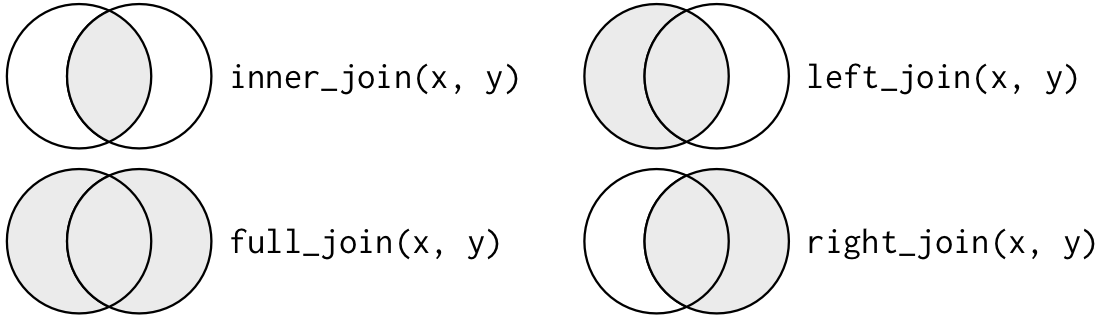
\includegraphics[width=0.7\linewidth]{img/cap05_fig03} 

}

\caption{Diferentes tipos de joins, representados com um diagrama de Venn. Adaptado de: @wickham2017.}\label{fig:fig-r-join}
\end{figure}

Considerando a nomenclatura de duas tabelas de dados por \texttt{x} e \texttt{y}, temos:

\begin{itemize}
\tightlist
\item
  \texttt{inner\_join(x,\ y)}: mantém apenas as observações em \texttt{x} e em \texttt{y}
\item
  \texttt{left\_join(x,\ y)}: mantém todas as observações em \texttt{x}
\item
  \texttt{right\_join(x,\ y)}: mantém todas as observações em \texttt{y}
\item
  \texttt{full\_join(x,\ y)}: mantém todas as observações em \texttt{x} e em \texttt{y}
\end{itemize}

Aqui, vamos demostrar apenas a função \texttt{dplyr::left\_join()}, combinando um \texttt{tibble} de coordenadas geográficas das ilhas com o conjunto de dados do penguins.

\begin{Shaded}
\begin{Highlighting}[]
\DocumentationTok{\#\# Adicionar uma coluna chave de ids}
\NormalTok{penguin\_islands }\OtherTok{\textless{}{-}} \FunctionTok{tibble}\NormalTok{(}
  \AttributeTok{island =} \FunctionTok{c}\NormalTok{(}\StringTok{"Torgersen"}\NormalTok{, }\StringTok{"Biscoe"}\NormalTok{, }\StringTok{"Dream"}\NormalTok{, }\StringTok{"Alpha"}\NormalTok{),}
  \AttributeTok{longitude =} \FunctionTok{c}\NormalTok{(}\SpecialCharTok{{-}}\FloatTok{64.083333}\NormalTok{, }\SpecialCharTok{{-}}\FloatTok{63.775636}\NormalTok{, }\SpecialCharTok{{-}}\FloatTok{64.233333}\NormalTok{, }\SpecialCharTok{{-}}\DecValTok{63}\NormalTok{),}
  \AttributeTok{latitude =} \FunctionTok{c}\NormalTok{(}\SpecialCharTok{{-}}\FloatTok{64.766667}\NormalTok{, }\SpecialCharTok{{-}}\FloatTok{64.818569}\NormalTok{, }\SpecialCharTok{{-}}\FloatTok{64.733333}\NormalTok{, }\SpecialCharTok{{-}}\FloatTok{64.316667}\NormalTok{))}
  
\DocumentationTok{\#\# Junção {-} left}
\NormalTok{penguins\_left\_join }\OtherTok{\textless{}{-}}\NormalTok{ dplyr}\SpecialCharTok{::}\FunctionTok{left\_join}\NormalTok{(penguins, penguin\_islands, }\AttributeTok{by =} \StringTok{"island"}\NormalTok{)}
\FunctionTok{head}\NormalTok{(penguins\_left\_join)}
\CommentTok{\#\textgreater{} \# A tibble: 6 x 10}
\CommentTok{\#\textgreater{}   species island bill\_length\_mm bill\_depth\_mm flipper\_length\_\textasciitilde{} body\_mass\_g sex  }
\CommentTok{\#\textgreater{}   \textless{}fct\textgreater{}   \textless{}chr\textgreater{}           \textless{}dbl\textgreater{}         \textless{}dbl\textgreater{}            \textless{}int\textgreater{}       \textless{}int\textgreater{} \textless{}fct\textgreater{}}
\CommentTok{\#\textgreater{} 1 Adelie  Torge\textasciitilde{}           39.1          18.7              181        3750 male }
\CommentTok{\#\textgreater{} 2 Adelie  Torge\textasciitilde{}           39.5          17.4              186        3800 fema\textasciitilde{}}
\CommentTok{\#\textgreater{} 3 Adelie  Torge\textasciitilde{}           40.3          18                195        3250 fema\textasciitilde{}}
\CommentTok{\#\textgreater{} 4 Adelie  Torge\textasciitilde{}           NA            NA                 NA          NA NA   }
\CommentTok{\#\textgreater{} 5 Adelie  Torge\textasciitilde{}           36.7          19.3              193        3450 fema\textasciitilde{}}
\CommentTok{\#\textgreater{} 6 Adelie  Torge\textasciitilde{}           39.3          20.6              190        3650 male }
\CommentTok{\#\textgreater{} \# ... with 3 more variables: year \textless{}int\textgreater{}, longitude \textless{}dbl\textgreater{}, latitude \textless{}dbl\textgreater{}}
\end{Highlighting}
\end{Shaded}

Já a junção de filtragem combina as observações da mesma maneira que as junções de mutação, mas afetam as observações (linhas), não as variáveis (colunas). Existem dois tipos.

\begin{itemize}
\tightlist
\item
  \texttt{semi\_join(x,\ y)}: mantém todas as observações em \texttt{x} que têm uma correspondência em \texttt{y}
\item
  \texttt{anti\_join(x,\ y)}: elimina todas as observações em \texttt{x} que têm uma correspondência em \texttt{y}
\end{itemize}

\emph{Semi-joins} são úteis para corresponder tabelas de resumo filtradas de volta às linhas originais, removendo as linhas que não estavam antes do join. \emph{Anti-joins} são úteis para diagnosticar incompatibilidades de junção, por exemplo, ao verificar os elementos que não combinam entre duas tabelas de dados.

\hypertarget{operauxe7uxf5es-de-conjuntos-e-comparauxe7uxe3o-de-dados}{%
\subsection{Operações de conjuntos e comparação de dados}\label{operauxe7uxf5es-de-conjuntos-e-comparauxe7uxe3o-de-dados}}

Temos ainda operações de conjuntos e comparação de dados.

\begin{itemize}
\tightlist
\item
  \texttt{union(x,\ y)}: retorna todas as linhas que aparecem em \texttt{x}, \texttt{y} ou mais dos conjuntos de dados
\item
  \texttt{interesect(x,\ y)}: retorna apenas as linhas que aparecem em \texttt{x} e em \texttt{y}
\item
  \texttt{setdiff(x,\ y)}: retorna as linhas que aparecem \texttt{x}, mas não em \texttt{y}
\item
  \texttt{setequal(x,\ y)}: retorna se \texttt{x} e \texttt{y} são iguais e quais suas diferenças
\end{itemize}

Para se aprofundar no tema, recomendamos a leitura do Capítulo \href{https://r4ds.had.co.nz/relational-data.html}{13 Relational data} de \citet{wickham2017}.

\hypertarget{stringr}{%
\section{stringr}\label{stringr}}

O pacote \texttt{stringr} fornece um conjunto de funções para a manipulação de caracteres ou strings. O pacote concentra-se nas funções de manipulação mais importantes e comumente usadas. Para funções mais específicas, recomenda-se usar o pacote \texttt{stringi}, que fornece um conjunto mais abrangente de funções. As funções do \texttt{stringr} podem ser agrupadas em algumas operações para tarefas específicas como correspondência de padrões, retirar e acrescentar espaços em branco, mudar maiúsculas e minúsculas, além de outras operações.

Todas as funções deste pacote são listadas na \href{https://stringr.tidyverse.org/reference/index.html}{página de referência} do pacote.

Demonstraremos algumas funções para algumas operações mais comuns, utilizando um vetor de um elemento, com o string ``penguins''.

Podemos explorar o comprimento de strings com a função \texttt{stringr::str\_length()}.

\begin{Shaded}
\begin{Highlighting}[]
\DocumentationTok{\#\# Comprimento}
\NormalTok{stringr}\SpecialCharTok{::}\FunctionTok{str\_length}\NormalTok{(}\AttributeTok{string =} \StringTok{"penguins"}\NormalTok{)}
\CommentTok{\#\textgreater{} [1] 8}
\end{Highlighting}
\end{Shaded}

Extrair um string por sua posição usando a função \texttt{stringr::str\_sub()} ou por um padrão com \texttt{stringr::str\_extract()}.

\begin{Shaded}
\begin{Highlighting}[]
\DocumentationTok{\#\# Extrair pela posição}
\NormalTok{stringr}\SpecialCharTok{::}\FunctionTok{str\_sub}\NormalTok{(}\AttributeTok{string =} \StringTok{"penguins"}\NormalTok{, }\AttributeTok{end =} \DecValTok{3}\NormalTok{)}
\CommentTok{\#\textgreater{} [1] "pen"}

\DocumentationTok{\#\# Extrair por padrão}
\NormalTok{stringr}\SpecialCharTok{::}\FunctionTok{str\_extract}\NormalTok{(}\AttributeTok{string =} \StringTok{"penguins"}\NormalTok{, }\AttributeTok{pattern =} \StringTok{"p"}\NormalTok{)}
\CommentTok{\#\textgreater{} [1] "p"}
\end{Highlighting}
\end{Shaded}

Substituir strings por outros strings com \texttt{stringr::str\_replace()}.

\begin{Shaded}
\begin{Highlighting}[]
\DocumentationTok{\#\# Substituir}
\NormalTok{stringr}\SpecialCharTok{::}\FunctionTok{str\_replace}\NormalTok{(}\AttributeTok{string =} \StringTok{"penguins"}\NormalTok{, }\AttributeTok{pattern =} \StringTok{"i"}\NormalTok{, }\AttributeTok{replacement =} \StringTok{"y"}\NormalTok{)}
\CommentTok{\#\textgreater{} [1] "penguyns"}
\end{Highlighting}
\end{Shaded}

Separar strings por um padrão com a função \texttt{stringr::str\_split()}.

\begin{Shaded}
\begin{Highlighting}[]
\DocumentationTok{\#\# Separar}
\NormalTok{stringr}\SpecialCharTok{::}\FunctionTok{str\_split}\NormalTok{(}\AttributeTok{string =} \StringTok{"p{-}e{-}n{-}g{-}u{-}i{-}n{-}s"}\NormalTok{, }\AttributeTok{pattern =} \StringTok{"{-}"}\NormalTok{, }\AttributeTok{simplify =} \ConstantTok{TRUE}\NormalTok{)}
\CommentTok{\#\textgreater{}      [,1] [,2] [,3] [,4] [,5] [,6] [,7] [,8]}
\CommentTok{\#\textgreater{} [1,] "p"  "e"  "n"  "g"  "u"  "i"  "n"  "s"}
\end{Highlighting}
\end{Shaded}

Inserir espaços em brancos pela esquerda, direita ou ambos com a função \texttt{stringr::str\_pad()}.

\begin{Shaded}
\begin{Highlighting}[]
\DocumentationTok{\#\# Inserir espacos em branco}
\NormalTok{stringr}\SpecialCharTok{::}\FunctionTok{str\_pad}\NormalTok{(}\AttributeTok{string =} \StringTok{"penguins"}\NormalTok{, }\AttributeTok{width =} \DecValTok{10}\NormalTok{, }\AttributeTok{side =} \StringTok{"left"}\NormalTok{)}
\CommentTok{\#\textgreater{} [1] "  penguins"}
\NormalTok{stringr}\SpecialCharTok{::}\FunctionTok{str\_pad}\NormalTok{(}\AttributeTok{string =} \StringTok{"penguins"}\NormalTok{, }\AttributeTok{width =} \DecValTok{10}\NormalTok{, }\AttributeTok{side =} \StringTok{"right"}\NormalTok{)}
\CommentTok{\#\textgreater{} [1] "penguins  "}
\NormalTok{stringr}\SpecialCharTok{::}\FunctionTok{str\_pad}\NormalTok{(}\AttributeTok{string =} \StringTok{"penguins"}\NormalTok{, }\AttributeTok{width =} \DecValTok{10}\NormalTok{, }\AttributeTok{side =} \StringTok{"both"}\NormalTok{)}
\CommentTok{\#\textgreater{} [1] " penguins "}
\end{Highlighting}
\end{Shaded}

Também podemos remover espaços em branco da esquerda, direita ou ambos, utilizando \texttt{stringr::str\_trim()}.

\begin{Shaded}
\begin{Highlighting}[]
\DocumentationTok{\#\# Remover espacos em branco}
\NormalTok{stringr}\SpecialCharTok{::}\FunctionTok{str\_trim}\NormalTok{(}\AttributeTok{string =} \StringTok{" penguins "}\NormalTok{, }\AttributeTok{side =} \StringTok{"left"}\NormalTok{)}
\CommentTok{\#\textgreater{} [1] "penguins "}
\NormalTok{stringr}\SpecialCharTok{::}\FunctionTok{str\_trim}\NormalTok{(}\AttributeTok{string =} \StringTok{" penguins "}\NormalTok{, }\AttributeTok{side =} \StringTok{"right"}\NormalTok{)}
\CommentTok{\#\textgreater{} [1] " penguins"}
\NormalTok{stringr}\SpecialCharTok{::}\FunctionTok{str\_trim}\NormalTok{(}\AttributeTok{string =} \StringTok{" penguins "}\NormalTok{, }\AttributeTok{side =} \StringTok{"both"}\NormalTok{)}
\CommentTok{\#\textgreater{} [1] "penguins"}
\end{Highlighting}
\end{Shaded}

Podemos também alterar minúsculas e maiúsculas em diferentes posições do string, com várias funções.

\begin{Shaded}
\begin{Highlighting}[]
\DocumentationTok{\#\# Alterar minúsculas e maiúsculas}
\NormalTok{stringr}\SpecialCharTok{::}\FunctionTok{str\_to\_lower}\NormalTok{(}\AttributeTok{string =} \StringTok{"Penguins"}\NormalTok{)}
\CommentTok{\#\textgreater{} [1] "penguins"}
\NormalTok{stringr}\SpecialCharTok{::}\FunctionTok{str\_to\_upper}\NormalTok{(}\AttributeTok{string =} \StringTok{"penguins"}\NormalTok{)}
\CommentTok{\#\textgreater{} [1] "PENGUINS"}
\NormalTok{stringr}\SpecialCharTok{::}\FunctionTok{str\_to\_sentence}\NormalTok{(}\AttributeTok{string =} \StringTok{"penGuins"}\NormalTok{)}
\CommentTok{\#\textgreater{} [1] "Penguins"}
\NormalTok{stringr}\SpecialCharTok{::}\FunctionTok{str\_to\_title}\NormalTok{(}\AttributeTok{string =} \StringTok{"penGuins"}\NormalTok{)}
\CommentTok{\#\textgreater{} [1] "Penguins"}
\end{Highlighting}
\end{Shaded}

Podemos ainda ordenar os elementos de um vetor por ordem alfabética de forma crescente ou decrescente, usando \texttt{stringr::str\_sort()}.

\begin{Shaded}
\begin{Highlighting}[]
\DocumentationTok{\#\# Ordenar}
\NormalTok{stringr}\SpecialCharTok{::}\FunctionTok{str\_sort}\NormalTok{(}\AttributeTok{x =}\NormalTok{ letters)}
\CommentTok{\#\textgreater{}  [1] "a" "b" "c" "d" "e" "f" "g" "h" "i" "j" "k" "l" "m" "n" "o" "p" "q" "r" "s"}
\CommentTok{\#\textgreater{} [20] "t" "u" "v" "w" "x" "y" "z"}
\NormalTok{stringr}\SpecialCharTok{::}\FunctionTok{str\_sort}\NormalTok{(}\AttributeTok{x =}\NormalTok{ letters, }\AttributeTok{dec =} \ConstantTok{TRUE}\NormalTok{)}
\CommentTok{\#\textgreater{}  [1] "z" "y" "x" "w" "v" "u" "t" "s" "r" "q" "p" "o" "n" "m" "l" "k" "j" "i" "h"}
\CommentTok{\#\textgreater{} [20] "g" "f" "e" "d" "c" "b" "a"}
\end{Highlighting}
\end{Shaded}

Podemos ainda utilizar essas funções em complemento com o pacote \texttt{dplyr}, para alterar os strings de colunas ou nome das colunas.

\begin{Shaded}
\begin{Highlighting}[]
\DocumentationTok{\#\# Alterar valores das colunas}
\NormalTok{penguins\_stringr\_valores }\OtherTok{\textless{}{-}}\NormalTok{ penguins }\SpecialCharTok{\%\textgreater{}\%} 
\NormalTok{  dplyr}\SpecialCharTok{::}\FunctionTok{mutate}\NormalTok{(}\AttributeTok{species =}\NormalTok{ stringr}\SpecialCharTok{::}\FunctionTok{str\_to\_lower}\NormalTok{(species))}

\DocumentationTok{\#\# Alterar nome das colunas}
\NormalTok{penguins\_stringr\_nomes }\OtherTok{\textless{}{-}}\NormalTok{ penguins }\SpecialCharTok{\%\textgreater{}\%} 
\NormalTok{  dplyr}\SpecialCharTok{::}\FunctionTok{rename\_with}\NormalTok{(stringr}\SpecialCharTok{::}\NormalTok{str\_to\_title)}
\end{Highlighting}
\end{Shaded}

Para se aprofundar no tema, recomendamos a leitura do Capítulo \href{https://r4ds.had.co.nz/strings.html}{14 Strings} de \citet{wickham2017}.

\hypertarget{forcats}{%
\section{forcats}\label{forcats}}

O pacote \texttt{forcats} fornece um conjunto de ferramentas úteis para facilitar a manipulação de fatores. Como dito anteriormente, usamos fatores geralmente quando temos dados categóricos, que são variáveis que possuem um conjunto de valores fixos e conhecidos. As funções são utilizadas principalmente para: mudar a ordem dos níveis, mudar os valores dos níveis, adicionar e remover níveis, combinar múltiplos níveis, além de outras operações.

Todas as funções deste pacote são listadas na \href{https://forcats.tidyverse.org/reference/index.html}{página de referência} do pacote.

Vamos utilizar ainda os dados penguins e penguins\_raw para exemplificar o uso do pacote \texttt{forcats}.

\begin{Shaded}
\begin{Highlighting}[]
\DocumentationTok{\#\# Carregar o pacote palmerpenguins}
\FunctionTok{library}\NormalTok{(palmerpenguins)}
\end{Highlighting}
\end{Shaded}

Primeiramente, vamos converter dados de string para fator, utilizando a função \texttt{forcats::as\_factor()}.

\begin{Shaded}
\begin{Highlighting}[]
\DocumentationTok{\#\# String}
\NormalTok{forcats}\SpecialCharTok{::}\FunctionTok{as\_factor}\NormalTok{(penguins\_raw}\SpecialCharTok{$}\NormalTok{Species) }\SpecialCharTok{\%\textgreater{}\%} \FunctionTok{head}\NormalTok{()}
\CommentTok{\#\textgreater{} [1] Adelie Penguin (Pygoscelis adeliae) Adelie Penguin (Pygoscelis adeliae)}
\CommentTok{\#\textgreater{} [3] Adelie Penguin (Pygoscelis adeliae) Adelie Penguin (Pygoscelis adeliae)}
\CommentTok{\#\textgreater{} [5] Adelie Penguin (Pygoscelis adeliae) Adelie Penguin (Pygoscelis adeliae)}
\CommentTok{\#\textgreater{} 3 Levels: Adelie Penguin (Pygoscelis adeliae) ...}
\end{Highlighting}
\end{Shaded}

Podemos facilmente mudar o nome dos níveis utilizando a função \texttt{forcats::fct\_recode()}.

\begin{Shaded}
\begin{Highlighting}[]
\DocumentationTok{\#\# Mudar o nome dos níveis}
\NormalTok{forcats}\SpecialCharTok{::}\FunctionTok{fct\_recode}\NormalTok{(penguins}\SpecialCharTok{$}\NormalTok{species, }\AttributeTok{a =} \StringTok{"Adelie"}\NormalTok{, }\AttributeTok{c =} \StringTok{"Chinstrap"}\NormalTok{, }\AttributeTok{g =} \StringTok{"Gentoo"}\NormalTok{) }\SpecialCharTok{\%\textgreater{}\%} \FunctionTok{head}\NormalTok{()}
\CommentTok{\#\textgreater{} [1] a a a a a a}
\CommentTok{\#\textgreater{} Levels: a c g}
\end{Highlighting}
\end{Shaded}

Para inverter os níveis, usamos a função \texttt{forcats::fct\_rev()}.

\begin{Shaded}
\begin{Highlighting}[]
\DocumentationTok{\#\# Inverter os níveis}
\NormalTok{forcats}\SpecialCharTok{::}\FunctionTok{fct\_rev}\NormalTok{(penguins}\SpecialCharTok{$}\NormalTok{species) }\SpecialCharTok{\%\textgreater{}\%} \FunctionTok{head}\NormalTok{()}
\CommentTok{\#\textgreater{} [1] Adelie Adelie Adelie Adelie Adelie Adelie}
\CommentTok{\#\textgreater{} Levels: Gentoo Chinstrap Adelie}
\end{Highlighting}
\end{Shaded}

Uma operação muito comum com fatores é mudar a ordem dos níveis. Quando precisamos especificar a ordem dos níveis, podemos fazer essa operação manualmente com a função \texttt{forcats::fct\_relevel()}.

\begin{Shaded}
\begin{Highlighting}[]
\DocumentationTok{\#\# Especificar a ordem dos níveis}
\NormalTok{forcats}\SpecialCharTok{::}\FunctionTok{fct\_relevel}\NormalTok{(penguins}\SpecialCharTok{$}\NormalTok{species, }\StringTok{"Chinstrap"}\NormalTok{, }\StringTok{"Gentoo"}\NormalTok{, }\StringTok{"Adelie"}\NormalTok{) }\SpecialCharTok{\%\textgreater{}\%} \FunctionTok{head}\NormalTok{()}
\CommentTok{\#\textgreater{} [1] Adelie Adelie Adelie Adelie Adelie Adelie}
\CommentTok{\#\textgreater{} Levels: Chinstrap Gentoo Adelie}
\end{Highlighting}
\end{Shaded}

Como vimos, a reordenação dos níveis pode ser feita manualmente. Mas existem outras formas automáticas de reordenação seguindo algumas regras, para as quais existem funções específicas.

\begin{itemize}
\tightlist
\item
  \texttt{forcats::fct\_inorder()}: pela ordem em que aparecem pela primeira vez
\item
  \texttt{forcats::fct\_infreq()}: por número de observações com cada nível (decrescente, i.e., o maior primeiro)
\item
  \texttt{forcats::fct\_inseq()}: pelo valor numérico do nível
\end{itemize}

\begin{Shaded}
\begin{Highlighting}[]
\DocumentationTok{\#\# Níveis pela ordem em que aparecem}
\NormalTok{forcats}\SpecialCharTok{::}\FunctionTok{fct\_inorder}\NormalTok{(penguins}\SpecialCharTok{$}\NormalTok{species) }\SpecialCharTok{\%\textgreater{}\%} \FunctionTok{head}\NormalTok{()}
\CommentTok{\#\textgreater{} [1] Adelie Adelie Adelie Adelie Adelie Adelie}
\CommentTok{\#\textgreater{} Levels: Adelie Gentoo Chinstrap}

\DocumentationTok{\#\# Ordem (decrescente) de frequência}
\NormalTok{forcats}\SpecialCharTok{::}\FunctionTok{fct\_infreq}\NormalTok{(penguins}\SpecialCharTok{$}\NormalTok{species) }\SpecialCharTok{\%\textgreater{}\%} \FunctionTok{head}\NormalTok{()}
\CommentTok{\#\textgreater{} [1] Adelie Adelie Adelie Adelie Adelie Adelie}
\CommentTok{\#\textgreater{} Levels: Adelie Gentoo Chinstrap}
\end{Highlighting}
\end{Shaded}

Por fim, podemos fazer a agregação de níveis raros em um nível utilizando a função \texttt{forcats::fct\_lump()}.

\begin{Shaded}
\begin{Highlighting}[]
\DocumentationTok{\#\# Agregação de níveis raros em um nível}
\NormalTok{forcats}\SpecialCharTok{::}\FunctionTok{fct\_lump}\NormalTok{(penguins}\SpecialCharTok{$}\NormalTok{species) }\SpecialCharTok{\%\textgreater{}\%} \FunctionTok{head}\NormalTok{()}
\CommentTok{\#\textgreater{} [1] Adelie Adelie Adelie Adelie Adelie Adelie}
\CommentTok{\#\textgreater{} Levels: Adelie Gentoo Other}
\end{Highlighting}
\end{Shaded}

Podemos ainda utilizar essas funções em complemento com o pacote \texttt{dplyr} para fazer manipulações de fatores nas colunas de \texttt{tibbles}.

\begin{Shaded}
\begin{Highlighting}[]
\DocumentationTok{\#\# Transformar várias colunas em fator}
\NormalTok{penguins\_raw\_multi\_factor }\OtherTok{\textless{}{-}}\NormalTok{ penguins\_raw }\SpecialCharTok{\%\textgreater{}\%} 
\NormalTok{  dplyr}\SpecialCharTok{::}\FunctionTok{mutate}\NormalTok{(}\FunctionTok{across}\NormalTok{(}\FunctionTok{where}\NormalTok{(is.character), forcats}\SpecialCharTok{::}\NormalTok{as\_factor))}
\end{Highlighting}
\end{Shaded}

Para se aprofundar no tema, recomendamos a leitura do Capítulo \href{https://r4ds.had.co.nz/factors.html}{15 Factors} de \citet{wickham2017}.

\hypertarget{lubridate}{%
\section{lubridate}\label{lubridate}}

O pacote \texttt{lubridate} fornece um conjunto de funções para a manipulação de dados de data e horário. Dessa forma, esse pacote facilita a manipulação dessa classe de dado no R, pois geralmente esses dados não são intuitivos e mudam dependendo do tipo de objeto de data e horário. Além disso, os métodos que usam datas e horários devem levar em consideração fusos horários, anos bissextos, horários de verão, além de outras particularidades. Existem diversas funções nesse pacote, sendo as mesmas focadas em: transformações de data/horário, componentes, arredondamentos, durações, períodos, intervalos, além de muitas outras funções específicas.

Todas as funções deste pacote são listadas na \href{https://lubridate.tidyverse.org/reference/index.html}{página de referência} do pacote.

Apesar de estar inserido no escopo do \emph{tidyverse}, este pacote não é carregado com os demais, requisitando seu carregamento solo.

\begin{Shaded}
\begin{Highlighting}[]
\DocumentationTok{\#\# Carregar}
\FunctionTok{library}\NormalTok{(lubridate)}
\end{Highlighting}
\end{Shaded}

Existem três tipos de dados data/horário:

\begin{itemize}
\tightlist
\item
  \textbf{Data}: tempo em dias, meses e anos \texttt{\textless{}date\textgreater{}}
\item
  \textbf{Horário}: tempo dentro de um dia \texttt{\textless{}time\textgreater{}}
\item
  \textbf{Data-horário}: tempo em um instante (data mais tempo) \texttt{\textless{}dttm\textgreater{}}
\end{itemize}

Para trabalhar exclusivamente com horários, podemos utilizar o pacote \texttt{hms}.

É fundamental também destacar que algumas letras terão um significado temporal, sendo abreviações de diferentes períodos em inglês: \textbf{y}ear (ano), \textbf{m}onth (mês), \textbf{w}eak (semana), \textbf{d}ay (dia), \textbf{h}our (hora), \textbf{m}inute (minuto), e \textbf{s}econd (segundo).

Para acessar a informação da data e horários atuais podemos utilizar as funções \texttt{lubridate::today()} e \texttt{lubridate::now()}.

\begin{Shaded}
\begin{Highlighting}[]
\DocumentationTok{\#\# Extrair a data nesse instante}
\NormalTok{lubridate}\SpecialCharTok{::}\FunctionTok{today}\NormalTok{()}
\CommentTok{\#\textgreater{} [1] "2021{-}08{-}12"}

\DocumentationTok{\#\# Extrair a data e tempo nesse instante}
\NormalTok{lubridate}\SpecialCharTok{::}\FunctionTok{now}\NormalTok{()}
\CommentTok{\#\textgreater{} [1] "2021{-}08{-}12 14:26:11 CEST"}
\end{Highlighting}
\end{Shaded}

Além dessas informações instantâneas, existem três maneiras de criar um dado de data/horário.

\begin{itemize}
\tightlist
\item
  De um string
\item
  De componentes individuais de data e horário
\item
  De um objeto de data/horário existente
\end{itemize}

Os dados de data/horário geralmente estão no formato de strings. Podemos transformar os dados especificando a ordem dos seus componentes, ou seja, a ordem em que ano, mês e dia aparecem no string, usando as letras \texttt{y} (ano), \texttt{m} (mês) e \texttt{d} (dia) na mesma ordem, por exemplo, \texttt{lubridate::dmy()}.

\begin{Shaded}
\begin{Highlighting}[]
\DocumentationTok{\#\# Strings e números para datas}
\NormalTok{lubridate}\SpecialCharTok{::}\FunctionTok{dmy}\NormalTok{(}\StringTok{"03{-}03{-}2021"}\NormalTok{)}
\CommentTok{\#\textgreater{} [1] "2021{-}03{-}03"}
\end{Highlighting}
\end{Shaded}

Essas funções também aceitam números sem aspas, além de serem muito versáteis e funcionarem em outros diversos formatos.

\begin{Shaded}
\begin{Highlighting}[]
\DocumentationTok{\#\# Strings e números para datas}
\NormalTok{lubridate}\SpecialCharTok{::}\FunctionTok{dmy}\NormalTok{(}\StringTok{"03{-}Mar{-}2021"}\NormalTok{)}
\NormalTok{lubridate}\SpecialCharTok{::}\FunctionTok{dmy}\NormalTok{(}\DecValTok{03032021}\NormalTok{)}
\NormalTok{lubridate}\SpecialCharTok{::}\FunctionTok{dmy}\NormalTok{(}\StringTok{"03032021"}\NormalTok{)}
\NormalTok{lubridate}\SpecialCharTok{::}\FunctionTok{dmy}\NormalTok{(}\StringTok{"03/03/2021"}\NormalTok{)}
\NormalTok{lubridate}\SpecialCharTok{::}\FunctionTok{dmy}\NormalTok{(}\StringTok{"03.03.2021"}\NormalTok{)}
\end{Highlighting}
\end{Shaded}

Além da data, podemos especificar horários atrelados a essas datas. Para criar uma data com horário adicionamos um underscore (\texttt{\_}) e os \texttt{h} (hora), \texttt{m} (minuto) e \texttt{s} (segundo) ao nome da função, além do argumento \texttt{tz} para especificar o \emph{fuso horário} (tema tratado mais adiante nessa seção).

\begin{Shaded}
\begin{Highlighting}[]
\DocumentationTok{\#\# Especificar horários e fuso horário}
\NormalTok{lubridate}\SpecialCharTok{::}\FunctionTok{dmy\_h}\NormalTok{(}\StringTok{"03{-}03{-}2021 13"}\NormalTok{)}
\CommentTok{\#\textgreater{} [1] "2021{-}03{-}03 13:00:00 UTC"}
\NormalTok{lubridate}\SpecialCharTok{::}\FunctionTok{dmy\_hm}\NormalTok{(}\StringTok{"03{-}03{-}2021 13:32"}\NormalTok{)}
\CommentTok{\#\textgreater{} [1] "2021{-}03{-}03 13:32:00 UTC"}
\NormalTok{lubridate}\SpecialCharTok{::}\FunctionTok{dmy\_hms}\NormalTok{(}\StringTok{"03{-}03{-}2021 13:32:01"}\NormalTok{)}
\CommentTok{\#\textgreater{} [1] "2021{-}03{-}03 13:32:01 UTC"}
\NormalTok{lubridate}\SpecialCharTok{::}\FunctionTok{dmy\_hms}\NormalTok{(}\StringTok{"03{-}03{-}2021 13:32:01"}\NormalTok{, }\AttributeTok{tz =} \StringTok{"America/Sao\_Paulo"}\NormalTok{)}
\CommentTok{\#\textgreater{} [1] "2021{-}03{-}03 13:32:01 {-}03"}
\end{Highlighting}
\end{Shaded}

Podemos ainda ter componentes individuais de data/horário em múltiplas colunas. Para realizar essa transformação, podemos usar as funções \texttt{lubridate::make\_date()} e \texttt{lubridate::make\_datetime()}.

\begin{Shaded}
\begin{Highlighting}[]
\DocumentationTok{\#\# Dados com componentes individuais}
\NormalTok{dados }\OtherTok{\textless{}{-}}\NormalTok{ tibble}\SpecialCharTok{::}\FunctionTok{tibble}\NormalTok{(}
  \AttributeTok{ano =} \FunctionTok{c}\NormalTok{(}\DecValTok{2021}\NormalTok{, }\DecValTok{2021}\NormalTok{, }\DecValTok{2021}\NormalTok{),}
  \AttributeTok{mes =} \FunctionTok{c}\NormalTok{(}\DecValTok{1}\NormalTok{, }\DecValTok{2}\NormalTok{, }\DecValTok{3}\NormalTok{),}
  \AttributeTok{dia =} \FunctionTok{c}\NormalTok{(}\DecValTok{12}\NormalTok{, }\DecValTok{20}\NormalTok{, }\DecValTok{31}\NormalTok{),}
  \AttributeTok{hora =} \FunctionTok{c}\NormalTok{(}\DecValTok{2}\NormalTok{, }\DecValTok{14}\NormalTok{, }\DecValTok{18}\NormalTok{), }
  \AttributeTok{minuto =} \FunctionTok{c}\NormalTok{(}\DecValTok{2}\NormalTok{, }\DecValTok{44}\NormalTok{, }\DecValTok{55}\NormalTok{))}

\DocumentationTok{\#\# Data de componentes individuais}
\NormalTok{dados }\SpecialCharTok{\%\textgreater{}\%} 
\NormalTok{  dplyr}\SpecialCharTok{::}\FunctionTok{mutate}\NormalTok{(}\AttributeTok{data =}\NormalTok{ lubridate}\SpecialCharTok{::}\FunctionTok{make\_datetime}\NormalTok{(ano, mes, dia, hora, minuto))}
\CommentTok{\#\textgreater{} \# A tibble: 3 x 6}
\CommentTok{\#\textgreater{}     ano   mes   dia  hora minuto data               }
\CommentTok{\#\textgreater{}   \textless{}dbl\textgreater{} \textless{}dbl\textgreater{} \textless{}dbl\textgreater{} \textless{}dbl\textgreater{}  \textless{}dbl\textgreater{} \textless{}dttm\textgreater{}             }
\CommentTok{\#\textgreater{} 1  2021     1    12     2      2 2021{-}01{-}12 02:02:00}
\CommentTok{\#\textgreater{} 2  2021     2    20    14     44 2021{-}02{-}20 14:44:00}
\CommentTok{\#\textgreater{} 3  2021     3    31    18     55 2021{-}03{-}31 18:55:00}
\end{Highlighting}
\end{Shaded}

Por fim, podemo criar datas modificando entre data/horário e data, utilizando as funções \texttt{lubridate::as\_datetime()} e \texttt{lubridate::as\_date()}.

\begin{Shaded}
\begin{Highlighting}[]
\DocumentationTok{\#\# Data para data{-}horário}
\NormalTok{lubridate}\SpecialCharTok{::}\FunctionTok{as\_datetime}\NormalTok{(}\FunctionTok{today}\NormalTok{())}
\CommentTok{\#\textgreater{} [1] "2021{-}08{-}12 UTC"}

\DocumentationTok{\#\# Data{-}horário para data}
\NormalTok{lubridate}\SpecialCharTok{::}\FunctionTok{as\_date}\NormalTok{(}\FunctionTok{now}\NormalTok{())}
\CommentTok{\#\textgreater{} [1] "2021{-}08{-}12"}
\end{Highlighting}
\end{Shaded}

Uma vez que entendemos como podemos criar dados de data/horário, podemos explorar funções para acessar e definir componentes individuais. Para essa tarefa existe uma grande quantidade de funções para acessar de partes específicas de datas e horários.

\begin{itemize}
\tightlist
\item
  \texttt{year()}: acessa o ano
\item
  \texttt{month()}: acessa o mês
\item
  \texttt{month()}: acessa o dia
\item
  \texttt{yday()}: acessa o dia do ano
\item
  \texttt{mday()}: acessa o dia do mês
\item
  \texttt{wday()}: acessa o dia da semana
\item
  \texttt{hour()}: acessa as horas
\item
  \texttt{minute()}: acessa os minutos
\item
  \texttt{second()}: acessa os segundos
\end{itemize}

\begin{Shaded}
\begin{Highlighting}[]
\DocumentationTok{\#\# Extrair}
\NormalTok{lubridate}\SpecialCharTok{::}\FunctionTok{year}\NormalTok{(}\FunctionTok{now}\NormalTok{())}
\CommentTok{\#\textgreater{} [1] 2021}
\NormalTok{lubridate}\SpecialCharTok{::}\FunctionTok{month}\NormalTok{(}\FunctionTok{now}\NormalTok{())}
\CommentTok{\#\textgreater{} [1] 8}
\NormalTok{lubridate}\SpecialCharTok{::}\FunctionTok{month}\NormalTok{(}\FunctionTok{now}\NormalTok{(), }\AttributeTok{label =} \ConstantTok{TRUE}\NormalTok{)}
\CommentTok{\#\textgreater{} [1] Aug}
\CommentTok{\#\textgreater{} 12 Levels: Jan \textless{} Feb \textless{} Mar \textless{} Apr \textless{} May \textless{} Jun \textless{} Jul \textless{} Aug \textless{} Sep \textless{} ... \textless{} Dec}
\NormalTok{lubridate}\SpecialCharTok{::}\FunctionTok{day}\NormalTok{(}\FunctionTok{now}\NormalTok{())}
\CommentTok{\#\textgreater{} [1] 12}
\NormalTok{lubridate}\SpecialCharTok{::}\FunctionTok{wday}\NormalTok{(}\FunctionTok{now}\NormalTok{())}
\CommentTok{\#\textgreater{} [1] 5}
\NormalTok{lubridate}\SpecialCharTok{::}\FunctionTok{wday}\NormalTok{(}\FunctionTok{now}\NormalTok{(), }\AttributeTok{label =} \ConstantTok{TRUE}\NormalTok{)}
\CommentTok{\#\textgreater{} [1] Thu}
\CommentTok{\#\textgreater{} Levels: Sun \textless{} Mon \textless{} Tue \textless{} Wed \textless{} Thu \textless{} Fri \textless{} Sat}
\NormalTok{lubridate}\SpecialCharTok{::}\FunctionTok{second}\NormalTok{(}\FunctionTok{now}\NormalTok{())}
\CommentTok{\#\textgreater{} [1] 11.77395}
\end{Highlighting}
\end{Shaded}

Além de acessar componentes de datas e horários, podemos usar essas funções para fazer a inclusão de informações de datas e horários.

\begin{Shaded}
\begin{Highlighting}[]
\DocumentationTok{\#\# Data}
\NormalTok{data }\OtherTok{\textless{}{-}} \FunctionTok{dmy\_hms}\NormalTok{(}\StringTok{"04{-}03{-}2021 01:04:56"}\NormalTok{)}

\DocumentationTok{\#\# Incluir}
\NormalTok{lubridate}\SpecialCharTok{::}\FunctionTok{year}\NormalTok{(data) }\OtherTok{\textless{}{-}} \DecValTok{2020}
\NormalTok{lubridate}\SpecialCharTok{::}\FunctionTok{month}\NormalTok{(data) }\OtherTok{\textless{}{-}} \DecValTok{01}
\NormalTok{lubridate}\SpecialCharTok{::}\FunctionTok{hour}\NormalTok{(data) }\OtherTok{\textless{}{-}} \DecValTok{13}
\end{Highlighting}
\end{Shaded}

Mais convenientemente, podemos utilizar a função \texttt{update()} para alterar vários valores de uma vez.

\begin{Shaded}
\begin{Highlighting}[]
\DocumentationTok{\#\# Incluir vários valores}
\FunctionTok{update}\NormalTok{(data, }\AttributeTok{year =} \DecValTok{2020}\NormalTok{, }\AttributeTok{month =} \DecValTok{1}\NormalTok{, }\AttributeTok{mday =} \DecValTok{1}\NormalTok{, }\AttributeTok{hour =} \DecValTok{1}\NormalTok{)}
\CommentTok{\#\textgreater{} [1] "2020{-}01{-}01 01:04:56 UTC"}
\end{Highlighting}
\end{Shaded}

Muitas vezes precisamos fazer operações com datas, como a aritmética com datas: subtração, adição e divisão. Para tanto, é preciso entender três classes importantes que representam intervalos de tempo.

\begin{itemize}
\tightlist
\item
  \textbf{Durações}: representam um número exato de segundos
\item
  \textbf{Períodos}: representam unidades humanas como semanas e meses
\item
  \textbf{Intervalos}: representam um ponto inicial e final
\end{itemize}

Quando fazemos uma subtração de datas, criamos um objeto da classe \texttt{difftime}. Essa classe pode ser um pouco complicada de trabalhar, então dentro do \emph{lubridate}, podemos usar funções que convertem essa classe em duração, da classe \texttt{Duration}. As durações sempre registram o intervalo de tempo em segundos, com alguma unidade de tempo maior entre parênteses. Há uma série de funções para tratar dessa classe.

\begin{itemize}
\tightlist
\item
  \texttt{duration()}: cria data em duração
\item
  \texttt{as.duration()}: converte datas em duração
\item
  \texttt{dyears()}: duração de anos
\item
  \texttt{dmonths()}: duração de meses
\item
  \texttt{dweeks()}: duração de semanas
\item
  \texttt{ddays()}: duração de dias
\item
  \texttt{dhours()}: duração de horas
\item
  \texttt{dminutes()}: duração de minutos
\item
  \texttt{dseconds()}: duração de segundos
\end{itemize}

\begin{Shaded}
\begin{Highlighting}[]
\DocumentationTok{\#\# Subtração de datas}
\NormalTok{tempo\_estudando\_r }\OtherTok{\textless{}{-}}\NormalTok{ lubridate}\SpecialCharTok{::}\FunctionTok{today}\NormalTok{() }\SpecialCharTok{{-}}\NormalTok{ lubridate}\SpecialCharTok{::}\FunctionTok{dmy}\NormalTok{(}\StringTok{"30{-}11{-}2011"}\NormalTok{)}

\DocumentationTok{\#\# Conversão para duração}
\NormalTok{tempo\_estudando\_r\_dur }\OtherTok{\textless{}{-}}\NormalTok{ lubridate}\SpecialCharTok{::}\FunctionTok{as.duration}\NormalTok{(tempo\_estudando\_r)}

\DocumentationTok{\#\# Criando durações}
\NormalTok{lubridate}\SpecialCharTok{::}\FunctionTok{duration}\NormalTok{(}\DecValTok{90}\NormalTok{, }\StringTok{"seconds"}\NormalTok{)}
\CommentTok{\#\textgreater{} [1] "90s (\textasciitilde{}1.5 minutes)"}
\NormalTok{lubridate}\SpecialCharTok{::}\FunctionTok{duration}\NormalTok{(}\FloatTok{1.5}\NormalTok{, }\StringTok{"minutes"}\NormalTok{)}
\CommentTok{\#\textgreater{} [1] "90s (\textasciitilde{}1.5 minutes)"}
\NormalTok{lubridate}\SpecialCharTok{::}\FunctionTok{duration}\NormalTok{(}\DecValTok{1}\NormalTok{, }\StringTok{"days"}\NormalTok{)}
\CommentTok{\#\textgreater{} [1] "86400s (\textasciitilde{}1 days)"}

\DocumentationTok{\#\# Transformação da duração}
\NormalTok{lubridate}\SpecialCharTok{::}\FunctionTok{dseconds}\NormalTok{(}\DecValTok{100}\NormalTok{)}
\CommentTok{\#\textgreater{} [1] "100s (\textasciitilde{}1.67 minutes)"}
\NormalTok{lubridate}\SpecialCharTok{::}\FunctionTok{dminutes}\NormalTok{(}\DecValTok{100}\NormalTok{)}
\CommentTok{\#\textgreater{} [1] "6000s (\textasciitilde{}1.67 hours)"}
\NormalTok{lubridate}\SpecialCharTok{::}\FunctionTok{dhours}\NormalTok{(}\DecValTok{100}\NormalTok{)}
\CommentTok{\#\textgreater{} [1] "360000s (\textasciitilde{}4.17 days)"}
\NormalTok{lubridate}\SpecialCharTok{::}\FunctionTok{ddays}\NormalTok{(}\DecValTok{100}\NormalTok{)}
\CommentTok{\#\textgreater{} [1] "8640000s (\textasciitilde{}14.29 weeks)"}
\NormalTok{lubridate}\SpecialCharTok{::}\FunctionTok{dweeks}\NormalTok{(}\DecValTok{100}\NormalTok{)}
\CommentTok{\#\textgreater{} [1] "60480000s (\textasciitilde{}1.92 years)"}
\NormalTok{lubridate}\SpecialCharTok{::}\FunctionTok{dyears}\NormalTok{(}\DecValTok{100}\NormalTok{)}
\CommentTok{\#\textgreater{} [1] "3155760000s (\textasciitilde{}100 years)"}
\end{Highlighting}
\end{Shaded}

Podemos ainda utilizar as durações para fazer operações aritméticas com datas como adição, subtração e multiplicação.

\begin{Shaded}
\begin{Highlighting}[]
\DocumentationTok{\#\# Somando durações a datas}
\NormalTok{lubridate}\SpecialCharTok{::}\FunctionTok{today}\NormalTok{() }\SpecialCharTok{+}\NormalTok{ lubridate}\SpecialCharTok{::}\FunctionTok{ddays}\NormalTok{(}\DecValTok{1}\NormalTok{)}
\CommentTok{\#\textgreater{} [1] "2021{-}08{-}13"}

\DocumentationTok{\#\# Subtraindo durações de datas}
\NormalTok{lubridate}\SpecialCharTok{::}\FunctionTok{today}\NormalTok{() }\SpecialCharTok{{-}}\NormalTok{ lubridate}\SpecialCharTok{::}\FunctionTok{dyears}\NormalTok{(}\DecValTok{1}\NormalTok{)}
\CommentTok{\#\textgreater{} [1] "2020{-}08{-}11 18:00:00 UTC"}

\DocumentationTok{\#\# Multiplicando durações}
\DecValTok{2} \SpecialCharTok{*} \FunctionTok{dyears}\NormalTok{(}\DecValTok{2}\NormalTok{)}
\CommentTok{\#\textgreater{} [1] "126230400s (\textasciitilde{}4 years)"}
\end{Highlighting}
\end{Shaded}

Além das durações, podemos usar períodos, que são extensões de tempo não fixados em segundos como as durações, mas flexíveis, com o tempo em dias, semanas, meses ou anos, permitindo uma interpretação mais intuitiva das datas. Novamente, há uma série de funções para realizar essas operações.

\begin{itemize}
\tightlist
\item
  \texttt{period()}: cria data em período
\item
  \texttt{as.period()}: converte datas em período
\item
  \texttt{seconds()}: período em segundos
\item
  \texttt{minutes()}: período em minutos
\item
  \texttt{hours()}: período em horas
\item
  \texttt{days()}: período em dias
\item
  \texttt{weeks()}: período em semanas
\item
  \texttt{months()}: período em meses
\item
  \texttt{years()}: período em anos
\end{itemize}

\begin{Shaded}
\begin{Highlighting}[]
\DocumentationTok{\#\# Criando períodos}
\FunctionTok{period}\NormalTok{(}\FunctionTok{c}\NormalTok{(}\DecValTok{90}\NormalTok{, }\DecValTok{5}\NormalTok{), }\FunctionTok{c}\NormalTok{(}\StringTok{"second"}\NormalTok{, }\StringTok{"minute"}\NormalTok{))}
\CommentTok{\#\textgreater{} [1] "5M 90S"}
\FunctionTok{period}\NormalTok{(}\FunctionTok{c}\NormalTok{(}\DecValTok{3}\NormalTok{, }\DecValTok{1}\NormalTok{, }\DecValTok{2}\NormalTok{, }\DecValTok{13}\NormalTok{, }\DecValTok{1}\NormalTok{), }\FunctionTok{c}\NormalTok{(}\StringTok{"second"}\NormalTok{, }\StringTok{"minute"}\NormalTok{, }\StringTok{"hour"}\NormalTok{, }\StringTok{"day"}\NormalTok{, }\StringTok{"week"}\NormalTok{))}
\CommentTok{\#\textgreater{} [1] "20d 2H 1M 3S"}

\DocumentationTok{\#\# Transformação de períodos}
\NormalTok{lubridate}\SpecialCharTok{::}\FunctionTok{seconds}\NormalTok{(}\DecValTok{100}\NormalTok{)}
\CommentTok{\#\textgreater{} [1] "100S"}
\NormalTok{lubridate}\SpecialCharTok{::}\FunctionTok{minutes}\NormalTok{(}\DecValTok{100}\NormalTok{)}
\CommentTok{\#\textgreater{} [1] "100M 0S"}
\NormalTok{lubridate}\SpecialCharTok{::}\FunctionTok{hours}\NormalTok{(}\DecValTok{100}\NormalTok{)}
\CommentTok{\#\textgreater{} [1] "100H 0M 0S"}
\NormalTok{lubridate}\SpecialCharTok{::}\FunctionTok{days}\NormalTok{(}\DecValTok{100}\NormalTok{)}
\CommentTok{\#\textgreater{} [1] "100d 0H 0M 0S"}
\NormalTok{lubridate}\SpecialCharTok{::}\FunctionTok{weeks}\NormalTok{(}\DecValTok{100}\NormalTok{)}
\CommentTok{\#\textgreater{} [1] "700d 0H 0M 0S"}
\NormalTok{lubridate}\SpecialCharTok{::}\FunctionTok{years}\NormalTok{(}\DecValTok{100}\NormalTok{)}
\CommentTok{\#\textgreater{} [1] "100y 0m 0d 0H 0M 0S"}
\end{Highlighting}
\end{Shaded}

Além disso, podemos fazer operações com os períodos, somando e subtraindo.

\begin{Shaded}
\begin{Highlighting}[]
\DocumentationTok{\#\# Somando datas}
\NormalTok{lubridate}\SpecialCharTok{::}\FunctionTok{today}\NormalTok{() }\SpecialCharTok{+}\NormalTok{ lubridate}\SpecialCharTok{::}\FunctionTok{weeks}\NormalTok{(}\DecValTok{10}\NormalTok{)}
\CommentTok{\#\textgreater{} [1] "2021{-}10{-}21"}

\DocumentationTok{\#\# Subtraindo datas}
\NormalTok{lubridate}\SpecialCharTok{::}\FunctionTok{today}\NormalTok{() }\SpecialCharTok{{-}}\NormalTok{ lubridate}\SpecialCharTok{::}\FunctionTok{weeks}\NormalTok{(}\DecValTok{10}\NormalTok{)}
\CommentTok{\#\textgreater{} [1] "2021{-}06{-}03"}

\DocumentationTok{\#\# Criando datas recorrentes}
\NormalTok{lubridate}\SpecialCharTok{::}\FunctionTok{today}\NormalTok{() }\SpecialCharTok{+}\NormalTok{ lubridate}\SpecialCharTok{::}\FunctionTok{weeks}\NormalTok{(}\DecValTok{0}\SpecialCharTok{:}\DecValTok{10}\NormalTok{)}
\CommentTok{\#\textgreater{}  [1] "2021{-}08{-}12" "2021{-}08{-}19" "2021{-}08{-}26" "2021{-}09{-}02" "2021{-}09{-}09"}
\CommentTok{\#\textgreater{}  [6] "2021{-}09{-}16" "2021{-}09{-}23" "2021{-}09{-}30" "2021{-}10{-}07" "2021{-}10{-}14"}
\CommentTok{\#\textgreater{} [11] "2021{-}10{-}21"}
\end{Highlighting}
\end{Shaded}

Por fim, intervalos são períodos de tempo limitados por duas datas, possuindo uma duração com um ponto de partida, que o faz preciso para determinar uma duração. Intervalos são objetos da classe \texttt{Interval}. Da mesma forma que para duração e períodos, há uma série de funções para realizar essas operações.

\begin{itemize}
\tightlist
\item
  \texttt{interval()}: cria data em intervalo
\item
  \texttt{\%-\/-\%}: cria data em intervalo
\item
  \texttt{as.interval()}: converte datas em intervalo
\item
  \texttt{int\_start()}: acessa ou atribui data inicial de um intervalo
\item
  \texttt{int\_end()}: acessa ou atribui data final de um intervalo
\item
  \texttt{int\_length()}: comprimento de um intervalo em segundos
\item
  \texttt{int\_flip()}: inverte a ordem da data de início e da data de término em um intervalo
\item
  \texttt{int\_shift()}: desloca as datas de início e término de um intervalo
\item
  \texttt{int\_aligns()}: testa se dois intervalos compartilham um ponto final
\item
  \texttt{int\_standardize()}: garante que todos os intervalos sejam positivos
\item
  \texttt{int\_diff()}: retorna os intervalos que ocorrem entre os elementos de data/horário
\item
  \texttt{int\_overlaps()}: testa se dois intervalos se sobrepõem
\item
  \texttt{\%within\%}: testa se o primeiro intervalo está contido no segundo
\end{itemize}

\begin{Shaded}
\begin{Highlighting}[]
\DocumentationTok{\#\# Criando duas datas {-} início de estudos do R e nascimento do meu filho}
\NormalTok{r\_inicio }\OtherTok{\textless{}{-}}\NormalTok{ lubridate}\SpecialCharTok{::}\FunctionTok{dmy}\NormalTok{(}\StringTok{"30{-}11{-}2011"}\NormalTok{)}
\NormalTok{filho\_nascimento }\OtherTok{\textless{}{-}}\NormalTok{ lubridate}\SpecialCharTok{::}\FunctionTok{dmy}\NormalTok{(}\StringTok{"26{-}09{-}2013"}\NormalTok{)}
\NormalTok{r\_hoje }\OtherTok{\textless{}{-}}\NormalTok{ lubridate}\SpecialCharTok{::}\FunctionTok{today}\NormalTok{()}

\DocumentationTok{\#\# Criando intervalos {-} interval}
\NormalTok{r\_intervalo }\OtherTok{\textless{}{-}}\NormalTok{ lubridate}\SpecialCharTok{::}\FunctionTok{interval}\NormalTok{(r\_inicio, r\_hoje)}

\DocumentationTok{\#\# Criando intervalos {-} interval \%{-}{-}\%}
\NormalTok{filho\_intervalo }\OtherTok{\textless{}{-}}\NormalTok{ filho\_nascimento }\SpecialCharTok{\%{-}{-}\%}\NormalTok{ lubridate}\SpecialCharTok{::}\FunctionTok{today}\NormalTok{()}

\DocumentationTok{\#\# Operações com intervalos}
\NormalTok{lubridate}\SpecialCharTok{::}\FunctionTok{int\_start}\NormalTok{(r\_intervalo)}
\CommentTok{\#\textgreater{} [1] "2011{-}11{-}30 UTC"}
\NormalTok{lubridate}\SpecialCharTok{::}\FunctionTok{int\_end}\NormalTok{(r\_intervalo)}
\CommentTok{\#\textgreater{} [1] "2021{-}08{-}12 UTC"}
\NormalTok{lubridate}\SpecialCharTok{::}\FunctionTok{int\_length}\NormalTok{(r\_intervalo)}
\CommentTok{\#\textgreater{} [1] 306115200}
\NormalTok{lubridate}\SpecialCharTok{::}\FunctionTok{int\_flip}\NormalTok{(r\_intervalo)}
\CommentTok{\#\textgreater{} [1] 2021{-}08{-}12 UTC{-}{-}2011{-}11{-}30 UTC}
\NormalTok{lubridate}\SpecialCharTok{::}\FunctionTok{int\_shift}\NormalTok{(r\_intervalo, }\FunctionTok{duration}\NormalTok{(}\AttributeTok{days =} \DecValTok{30}\NormalTok{))}
\CommentTok{\#\textgreater{} [1] 2011{-}12{-}30 UTC{-}{-}2021{-}09{-}11 UTC}
\end{Highlighting}
\end{Shaded}

Uma operação de destaque é verificar a sobreposição entre dois intervalos.

\begin{Shaded}
\begin{Highlighting}[]
\DocumentationTok{\#\# Verificar sobreposição {-} int\_overlaps}
\NormalTok{lubridate}\SpecialCharTok{::}\FunctionTok{int\_overlaps}\NormalTok{(r\_intervalo, filho\_intervalo)}
\CommentTok{\#\textgreater{} [1] TRUE}

\DocumentationTok{\#\# Verificar se intervalo está contido}
\NormalTok{r\_intervalo }\SpecialCharTok{\%within\%}\NormalTok{ filho\_intervalo}
\CommentTok{\#\textgreater{} [1] FALSE}
\NormalTok{filho\_intervalo }\SpecialCharTok{\%within\%}\NormalTok{ r\_intervalo}
\CommentTok{\#\textgreater{} [1] TRUE}
\end{Highlighting}
\end{Shaded}

Podemos ainda calcular quantos períodos existem dentro de um intervalo, utilizando as operações de \texttt{/} e \texttt{\%/\%}.

\begin{Shaded}
\begin{Highlighting}[]
\DocumentationTok{\#\# Períodos dentro de um intervalo {-} anos}
\NormalTok{r\_intervalo }\SpecialCharTok{/}\NormalTok{ lubridate}\SpecialCharTok{::}\FunctionTok{years}\NormalTok{()}
\CommentTok{\#\textgreater{} [1] 9.69863}
\NormalTok{r\_intervalo }\SpecialCharTok{\%/\%}\NormalTok{ lubridate}\SpecialCharTok{::}\FunctionTok{years}\NormalTok{()}
\CommentTok{\#\textgreater{} [1] 9}

\DocumentationTok{\#\# Períodos dentro de um intervalo {-} dias e semandas}
\NormalTok{filho\_intervalo }\SpecialCharTok{/}\NormalTok{ lubridate}\SpecialCharTok{::}\FunctionTok{days}\NormalTok{()}
\CommentTok{\#\textgreater{} [1] 2877}
\NormalTok{filho\_intervalo }\SpecialCharTok{/}\NormalTok{ lubridate}\SpecialCharTok{::}\FunctionTok{weeks}\NormalTok{()}
\CommentTok{\#\textgreater{} [1] 411}
\end{Highlighting}
\end{Shaded}

Ainda podemos fazer transformações dos dados para períodos e ter todas as unidades de data e tempo que o intervalo compreende.

\begin{Shaded}
\begin{Highlighting}[]
\DocumentationTok{\#\# Tempo total estudando R}
\NormalTok{lubridate}\SpecialCharTok{::}\FunctionTok{as.period}\NormalTok{(r\_intervalo)}
\CommentTok{\#\textgreater{} [1] "9y 8m 13d 0H 0M 0S"}

\DocumentationTok{\#\# Idade do meu filho}
\NormalTok{lubridate}\SpecialCharTok{::}\FunctionTok{as.period}\NormalTok{(filho\_intervalo)}
\CommentTok{\#\textgreater{} [1] "7y 10m 17d 0H 0M 0S"}
\end{Highlighting}
\end{Shaded}

Por fim, fusos horários tendem a ser um fator complicador quando precisamos analisar informações instantâneas de tempo (horário) de outras partes do planeta, ou mesmo fazer conversões dos horários. No \texttt{lubridate} há funções para ajudar nesse sentido. Para isso, podemos utilizar a função \texttt{lubridate::with\_tz()}, e no argumento \texttt{tzone} informar o fuso horário para a transformação do horário.

Podemos descobrir o fuso horário que o R está considerando com a função \texttt{Sys.timezone()}.

\begin{Shaded}
\begin{Highlighting}[]
\DocumentationTok{\#\# Fuso horário no R}
\FunctionTok{Sys.timezone}\NormalTok{()}
\CommentTok{\#\textgreater{} [1] "Europe/Berlin"}
\end{Highlighting}
\end{Shaded}

No R há uma listagem dos nomes dos fusos horários que podemos utilizar no argumento \texttt{tzone} para diferentes fusos horários.

\begin{Shaded}
\begin{Highlighting}[]
\DocumentationTok{\#\# Verificar os fuso horários}
\FunctionTok{length}\NormalTok{(}\FunctionTok{OlsonNames}\NormalTok{())}
\CommentTok{\#\textgreater{} [1] 593}
\FunctionTok{head}\NormalTok{(}\FunctionTok{OlsonNames}\NormalTok{())}
\CommentTok{\#\textgreater{} [1] "Africa/Abidjan"     "Africa/Accra"       "Africa/Addis\_Ababa"}
\CommentTok{\#\textgreater{} [4] "Africa/Algiers"     "Africa/Asmara"      "Africa/Asmera"}
\end{Highlighting}
\end{Shaded}

Podemos nos perguntar que horas são em outra parte do globo ou fazer as conversões facilmente no \emph{lubridate}.

\begin{Shaded}
\begin{Highlighting}[]
\DocumentationTok{\#\# Que horas são em...}
\NormalTok{lubridate}\SpecialCharTok{::}\FunctionTok{with\_tz}\NormalTok{(lubridate}\SpecialCharTok{::}\FunctionTok{now}\NormalTok{(), }\AttributeTok{tzone =} \StringTok{"America/Sao\_Paulo"}\NormalTok{)}
\CommentTok{\#\textgreater{} [1] "2021{-}08{-}12 09:26:13 {-}03"}
\NormalTok{lubridate}\SpecialCharTok{::}\FunctionTok{with\_tz}\NormalTok{(lubridate}\SpecialCharTok{::}\FunctionTok{now}\NormalTok{(), }\AttributeTok{tzone =} \StringTok{"GMT"}\NormalTok{)}
\CommentTok{\#\textgreater{} [1] "2021{-}08{-}12 12:26:13 GMT"}
\NormalTok{lubridate}\SpecialCharTok{::}\FunctionTok{with\_tz}\NormalTok{(lubridate}\SpecialCharTok{::}\FunctionTok{now}\NormalTok{(), }\AttributeTok{tzone =} \StringTok{"Europe/Berlin"}\NormalTok{)}
\CommentTok{\#\textgreater{} [1] "2021{-}08{-}12 14:26:13 CEST"}

\DocumentationTok{\#\# Altera o fuso sem mudar a hora}
\NormalTok{lubridate}\SpecialCharTok{::}\FunctionTok{force\_tz}\NormalTok{(lubridate}\SpecialCharTok{::}\FunctionTok{now}\NormalTok{(), }\AttributeTok{tzone =} \StringTok{"GMT"}\NormalTok{)}
\CommentTok{\#\textgreater{} [1] "2021{-}08{-}12 14:26:13 GMT"}
\end{Highlighting}
\end{Shaded}

Para se aprofundar no tema, recomendamos a leitura do Capítulo \href{https://r4ds.had.co.nz/dates-and-times.html}{16 Dates and times} de \citet{wickham2017}.

\hypertarget{purrr}{%
\section{purrr}\label{purrr}}

O pacote \texttt{purrr} implementa a \emph{Programação Funcional} no R, fornecendo um conjunto completo e consistente de ferramentas para trabalhar com funções e vetores. A programação funcional é um assunto bastante extenso, sendo mais conhecido no R pela família de funções \texttt{purrr::map()}, que permite substituir muitos \emph{loops for} por um código mais sucinto e fácil de ler. Não focaremos aqui nas outras funções.

Todas as funções deste pacote são listadas na \href{https://purrr.tidyverse.org/reference/index.html}{página de referência} do pacote.

Um loop for pode ser entendido como uma iteração: um bloco de códigos é repetido mudando um contador de uma lista de possibilidades. Vamos exemplificar com uma iteração bem simples, onde imprimiremos no console os valores de 1 a 10, utilizando a função \texttt{for()}, um contador \texttt{i} em um vetor de dez números \texttt{1:10} que será iterado, no bloco de códigos definido entre \texttt{\{\}}, usando a função \texttt{print()} para imprimir os valores.

A ideia é bastante simples: a função \texttt{for()} vai atribuir o primeiro valor da lista ao contador \texttt{i}, esse contador será utilizado em todo o bloco de códigos. Quando o bloco terminar, o segundo valor é atribuído ao contador \texttt{i} e entra no bloco de códigos, repetindo esse processo até que todos os elementos da lista tenham sido atribuídos ao contador.

\begin{Shaded}
\begin{Highlighting}[]
\DocumentationTok{\#\# Loop for}
\ControlFlowTok{for}\NormalTok{(i }\ControlFlowTok{in} \DecValTok{1}\SpecialCharTok{:}\DecValTok{10}\NormalTok{)\{}
  \FunctionTok{print}\NormalTok{(i)}
\NormalTok{\}}
\CommentTok{\#\textgreater{} [1] 1}
\CommentTok{\#\textgreater{} [1] 2}
\CommentTok{\#\textgreater{} [1] 3}
\CommentTok{\#\textgreater{} [1] 4}
\CommentTok{\#\textgreater{} [1] 5}
\CommentTok{\#\textgreater{} [1] 6}
\CommentTok{\#\textgreater{} [1] 7}
\CommentTok{\#\textgreater{} [1] 8}
\CommentTok{\#\textgreater{} [1] 9}
\CommentTok{\#\textgreater{} [1] 10}
\end{Highlighting}
\end{Shaded}

Com essa ideia em mente, a programação funcional utilizando a função \texttt{purrr::map()}. O mesmo for ficaria dessa forma.

\begin{Shaded}
\begin{Highlighting}[]
\DocumentationTok{\#\# Loop for com map}
\NormalTok{purrr}\SpecialCharTok{::}\FunctionTok{map}\NormalTok{(}\AttributeTok{.x =} \DecValTok{1}\SpecialCharTok{:}\DecValTok{10}\NormalTok{, }\AttributeTok{.f =}\NormalTok{ print)}
\CommentTok{\#\textgreater{} [1] 1}
\CommentTok{\#\textgreater{} [1] 2}
\CommentTok{\#\textgreater{} [1] 3}
\CommentTok{\#\textgreater{} [1] 4}
\CommentTok{\#\textgreater{} [1] 5}
\CommentTok{\#\textgreater{} [1] 6}
\CommentTok{\#\textgreater{} [1] 7}
\CommentTok{\#\textgreater{} [1] 8}
\CommentTok{\#\textgreater{} [1] 9}
\CommentTok{\#\textgreater{} [1] 10}
\CommentTok{\#\textgreater{} [[1]]}
\CommentTok{\#\textgreater{} [1] 1}
\CommentTok{\#\textgreater{} }
\CommentTok{\#\textgreater{} [[2]]}
\CommentTok{\#\textgreater{} [1] 2}
\CommentTok{\#\textgreater{} }
\CommentTok{\#\textgreater{} [[3]]}
\CommentTok{\#\textgreater{} [1] 3}
\CommentTok{\#\textgreater{} }
\CommentTok{\#\textgreater{} [[4]]}
\CommentTok{\#\textgreater{} [1] 4}
\CommentTok{\#\textgreater{} }
\CommentTok{\#\textgreater{} [[5]]}
\CommentTok{\#\textgreater{} [1] 5}
\CommentTok{\#\textgreater{} }
\CommentTok{\#\textgreater{} [[6]]}
\CommentTok{\#\textgreater{} [1] 6}
\CommentTok{\#\textgreater{} }
\CommentTok{\#\textgreater{} [[7]]}
\CommentTok{\#\textgreater{} [1] 7}
\CommentTok{\#\textgreater{} }
\CommentTok{\#\textgreater{} [[8]]}
\CommentTok{\#\textgreater{} [1] 8}
\CommentTok{\#\textgreater{} }
\CommentTok{\#\textgreater{} [[9]]}
\CommentTok{\#\textgreater{} [1] 9}
\CommentTok{\#\textgreater{} }
\CommentTok{\#\textgreater{} [[10]]}
\CommentTok{\#\textgreater{} [1] 10}
\end{Highlighting}
\end{Shaded}

Nessa estrutura, temos:

\texttt{map(.x,\ .f)}

\begin{itemize}
\tightlist
\item
  \texttt{.x}: um vetor, lista ou data frame\\
\item
  \texttt{.f}: uma função
\end{itemize}

Num outro exemplo, aplicaremos a função \texttt{sum()} para somar os valores de vários elementos de uma lista.

\begin{Shaded}
\begin{Highlighting}[]
\DocumentationTok{\#\# Função map}
\NormalTok{x }\OtherTok{\textless{}{-}} \FunctionTok{list}\NormalTok{(}\DecValTok{1}\SpecialCharTok{:}\DecValTok{5}\NormalTok{, }\FunctionTok{c}\NormalTok{(}\DecValTok{4}\NormalTok{, }\DecValTok{5}\NormalTok{, }\DecValTok{7}\NormalTok{), }\FunctionTok{c}\NormalTok{(}\DecValTok{1}\NormalTok{, }\DecValTok{1}\NormalTok{, }\DecValTok{1}\NormalTok{), }\FunctionTok{c}\NormalTok{(}\DecValTok{2}\NormalTok{, }\DecValTok{2}\NormalTok{, }\DecValTok{2}\NormalTok{, }\DecValTok{2}\NormalTok{, }\DecValTok{2}\NormalTok{))}
\NormalTok{purrr}\SpecialCharTok{::}\FunctionTok{map}\NormalTok{(x, sum)}
\CommentTok{\#\textgreater{} [[1]]}
\CommentTok{\#\textgreater{} [1] 15}
\CommentTok{\#\textgreater{} }
\CommentTok{\#\textgreater{} [[2]]}
\CommentTok{\#\textgreater{} [1] 16}
\CommentTok{\#\textgreater{} }
\CommentTok{\#\textgreater{} [[3]]}
\CommentTok{\#\textgreater{} [1] 3}
\CommentTok{\#\textgreater{} }
\CommentTok{\#\textgreater{} [[4]]}
\CommentTok{\#\textgreater{} [1] 10}
\end{Highlighting}
\end{Shaded}

Há diferente tipos de retornos da família \texttt{purrr::map()}.

\begin{itemize}
\tightlist
\item
  \texttt{map()}: retorna uma lista
\item
  \texttt{map\_chr()}: retorna um vetor de strings
\item
  \texttt{map\_dbl()}: retorna um vetor numérico (double)
\item
  \texttt{map\_int()}: retorna um vetor numérico (integer)
\item
  \texttt{map\_lgl()}: retorna um vetor lógico
\item
  \texttt{map\_dfr()}: retorna um data frame (por linhas)
\item
  \texttt{map\_dfc()}: retorna um data frame (por colunas)
\end{itemize}

\begin{Shaded}
\begin{Highlighting}[]
\DocumentationTok{\#\# Variações da função map}
\NormalTok{purrr}\SpecialCharTok{::}\FunctionTok{map\_dbl}\NormalTok{(x, sum)}
\CommentTok{\#\textgreater{} [1] 15 16  3 10}
\NormalTok{purrr}\SpecialCharTok{::}\FunctionTok{map\_chr}\NormalTok{(x, paste, }\AttributeTok{collapse =} \StringTok{" "}\NormalTok{)}
\CommentTok{\#\textgreater{} [1] "1 2 3 4 5" "4 5 7"     "1 1 1"     "2 2 2 2 2"}
\end{Highlighting}
\end{Shaded}

Essas funcionalidades já eram conhecidas no Base R pelas funções da \emph{família \texttt{apply}}: \texttt{apply()}, \texttt{lapply()}, \texttt{sapply()}, \texttt{vapply()}, \texttt{mapply()}, \texttt{rapply()} e \texttt{tapply()}. Essas funções formam a base de combinações mais complexas e ajudam a realizar operações com poucas linhas de código, para diferentes retornos.

Temos ainda duas variantes da função \texttt{map()}: \texttt{purrr::map2()} e \texttt{purrr::pmap()}, para duas ou mais listas, respectivamente. Como vimos para a primeira função, existem várias variações do sufixo para modificar o retorno da função.

\begin{Shaded}
\begin{Highlighting}[]
\DocumentationTok{\#\# Listas}
\NormalTok{x }\OtherTok{\textless{}{-}} \FunctionTok{list}\NormalTok{(}\DecValTok{3}\NormalTok{, }\DecValTok{5}\NormalTok{, }\DecValTok{0}\NormalTok{, }\DecValTok{1}\NormalTok{)}
\NormalTok{y }\OtherTok{\textless{}{-}} \FunctionTok{list}\NormalTok{(}\DecValTok{3}\NormalTok{, }\DecValTok{5}\NormalTok{, }\DecValTok{0}\NormalTok{, }\DecValTok{1}\NormalTok{)}
\NormalTok{z }\OtherTok{\textless{}{-}} \FunctionTok{list}\NormalTok{(}\DecValTok{3}\NormalTok{, }\DecValTok{5}\NormalTok{, }\DecValTok{0}\NormalTok{, }\DecValTok{1}\NormalTok{)}

\DocumentationTok{\#\# Função map2}
\NormalTok{purrr}\SpecialCharTok{::}\FunctionTok{map2\_dbl}\NormalTok{(x, y, prod)}
\CommentTok{\#\textgreater{} [1]  9 25  0  1}

\DocumentationTok{\#\# Função pmap}
\NormalTok{purrr}\SpecialCharTok{::}\FunctionTok{pmap\_dbl}\NormalTok{(}\FunctionTok{list}\NormalTok{(x, y, z), prod)}
\CommentTok{\#\textgreater{} [1]  27 125   0   1}
\end{Highlighting}
\end{Shaded}

Essas funções podem ser usadas em conjunto para implementar rotinas de manipulação e análise de dados com poucas linhas de código, mas que não exploraremos em sua completude aqui. Listamos dois exemplos simples.

\begin{Shaded}
\begin{Highlighting}[]
\DocumentationTok{\#\# Resumo dos dados}
\NormalTok{penguins }\SpecialCharTok{\%\textgreater{}\%} 
\NormalTok{  dplyr}\SpecialCharTok{::}\FunctionTok{select}\NormalTok{(}\FunctionTok{where}\NormalTok{(is.numeric)) }\SpecialCharTok{\%\textgreater{}\%} 
\NormalTok{  tidyr}\SpecialCharTok{::}\FunctionTok{drop\_na}\NormalTok{() }\SpecialCharTok{\%\textgreater{}\%} 
\NormalTok{  purrr}\SpecialCharTok{::}\FunctionTok{map\_dbl}\NormalTok{(mean)}
\CommentTok{\#\textgreater{}    bill\_length\_mm     bill\_depth\_mm flipper\_length\_mm       body\_mass\_g }
\CommentTok{\#\textgreater{}          43.92193          17.15117         200.91520        4201.75439 }
\CommentTok{\#\textgreater{}              year }
\CommentTok{\#\textgreater{}        2008.02924}
\end{Highlighting}
\end{Shaded}

\begin{Shaded}
\begin{Highlighting}[]
\DocumentationTok{\#\# Análise dos dados}
\NormalTok{penguins }\SpecialCharTok{\%\textgreater{}\%}
\NormalTok{  dplyr}\SpecialCharTok{::}\FunctionTok{group\_split}\NormalTok{(island, species) }\SpecialCharTok{\%\textgreater{}\%} 
\NormalTok{  purrr}\SpecialCharTok{::}\FunctionTok{map}\NormalTok{(}\SpecialCharTok{\textasciitilde{}} \FunctionTok{lm}\NormalTok{(bill\_depth\_mm }\SpecialCharTok{\textasciitilde{}}\NormalTok{ bill\_length\_mm, }\AttributeTok{data =}\NormalTok{ .x)) }\SpecialCharTok{\%\textgreater{}\%} 
\NormalTok{  purrr}\SpecialCharTok{::}\FunctionTok{map}\NormalTok{(summary) }\SpecialCharTok{\%\textgreater{}\%} 
\NormalTok{  purrr}\SpecialCharTok{::}\FunctionTok{map}\NormalTok{(}\StringTok{"r.squared"}\NormalTok{)}
\CommentTok{\#\textgreater{} [[1]]}
\CommentTok{\#\textgreater{} [1] 0.2192052}
\CommentTok{\#\textgreater{} }
\CommentTok{\#\textgreater{} [[2]]}
\CommentTok{\#\textgreater{} [1] 0.4139429}
\CommentTok{\#\textgreater{} }
\CommentTok{\#\textgreater{} [[3]]}
\CommentTok{\#\textgreater{} [1] 0.2579242}
\CommentTok{\#\textgreater{} }
\CommentTok{\#\textgreater{} [[4]]}
\CommentTok{\#\textgreater{} [1] 0.4271096}
\CommentTok{\#\textgreater{} }
\CommentTok{\#\textgreater{} [[5]]}
\CommentTok{\#\textgreater{} [1] 0.06198376}
\end{Highlighting}
\end{Shaded}

Para se aprofundar no tema, recomendamos a leitura do Capítulo \href{https://r4ds.had.co.nz/iteration.html}{21 Iteration} de \citet{wickham2017}.

\hypertarget{exercuxedcios-1}{%
\section{Exercícios}\label{exercuxedcios-1}}

\begin{enumerate}
\def\labelenumi{\arabic{enumi}.}
\tightlist
\item
  Reescreva as operações abaixo utilizando pipes \texttt{\%\textgreater{}\%}.
\end{enumerate}

\begin{itemize}
\tightlist
\item
  \texttt{log10(cumsum(1:100))}
\item
  \texttt{sum(sqrt(abs(rnorm(100))))}
\item
  \texttt{sum(sort(sample(1:10,\ 10000,\ rep\ =\ TRUE)))}
\end{itemize}

\begin{enumerate}
\def\labelenumi{\arabic{enumi}.}
\setcounter{enumi}{1}
\item
  Use a função \texttt{download.file()} e \texttt{unzip()} para baixar e extrair o arquivo do data paper de médios e grandes mamíferos: \href{https://doi.org/10.1002/ecy.2785}{ATLANTIC MAMMALS}. Em seguinda, importe para o R, usando a função \texttt{readxl::read\_excel()}.
\item
  Use a função \texttt{tibble::glimpse()} para ter uma noção geral dos dados importados no item anterior.
\item
  Compare os dados de penguins (\emph{palmerpenguins::penguins\_raw} e \emph{palmerpenguins::penguins}). Monte uma série de funções dos pacotes \emph{tidyr} e \texttt{dplyr} para fazer limpar os dados e fazer com que o primeiro dado seja igual ao segundo.
\item
  Usando os dados de penguins (\emph{palmerpenguins::penguins}), calcule a correlação de Pearson entre comprimento e profundidade do bico para cada espécie e para todas as espécies. Compare os índices de correlação para exemplificar o Paradoxo de Simpsom.
\item
  Oficialmente a pandemia de COVID-19 começou no Brasil com o primeiro caso no dia 26 de fevereiro de 2020. Calcule quantos anos, meses, dias, semanas, horas, minutos e segundos se passou desde então. Calcule também quanto tempo se passou até você ser vacinado.
\end{enumerate}

\hypertarget{para-se-aprofundar-1}{%
\section{Para se aprofundar}\label{para-se-aprofundar-1}}

Listamos a seguir livros que recomendamos para seguir com sua aprendizagem em R e tidyverse.

\textbf{Português}

Damiani A, Milz B, Lente C, Falbel D, Correa F, Trecenti J, Luduvice N, Amorim W. 2021. Ciência de Dados em R. {[}\url{https://livro.curso-r.com/}{]}

Faria PD, Parga JPFA. 2020. Introdução à Linguagem R: seus fundamentos e sua prática. {[}\url{https://www.researchgate.net/publication/345985082_Introducao_a_Linguagem_R_seus_fundamentos_e_sua_pratica}{]}

Oliveira PF, Guerra S, Mcdonnell, R. 2018. Ciência de dados com R -- Introdução. IBPAD. {[}\url{https://cdr.ibpad.com.br/}{]}

\textbf{Inglês}

Grolemund G. 2017. The Essentials of Data Science: Knowledge Discovery Using R. Chapman and Hall/CRC.

Holmes S, Huber W. 2019. Modern Statistics for Modern Biology. Cambridge University Press. {[}\url{https://www.huber.embl.de/msmb/}{]}

Irizarry RA. 2019. Introduction to Data Science: Data Analysis and Prediction Algorithms with R. Chapman and Hall/CRC. {[}\url{https://rafalab.github.io/dsbook/}{]}

Ismay C., Kim AY. 2019. Statistical Inference via Data Science: A ModernDive into R and the Tidyverse. Chapman and Hall/CRC. {[}\url{https://moderndive.com/}{]}

Peng DP. 2020. R Programming for Data Science. {[}\url{https://bookdown.org/rdpeng/rprogdatascience/}{]}

Wickham H, Grolemund G. 2017. R for Data Science: Import, Tidy, Transform, Visualize, and Model Data. O'Reilly Media. {[}\url{https://r4ds.had.co.nz/}{]}

Wright C, Ellis S, Hicks S \& Peng R D. 2021. Tidyverse Skills for Data Science in R. {[}\url{https://jhudatascience.org/tidyversecourse/}{]}

Zumel N, Mount J. 2014. Practical Data Science with R Paperback. Manning.

\hypertarget{cap6}{%
\chapter{Guia de bolso de gráficos no R}\label{cap6}}

\hypertarget{introduuxe7uxe3o-2}{%
\section{1. Introdução}\label{introduuxe7uxe3o-2}}

A visualização de dados através de gráficos geralmente é a melhor forma de apresentar e interpretar as informações contidas em seus estudos, fazendo uma uma síntese para melhor entendimento de padrões. Geralmente, os gráficos são necessários em quase todas as análises estatísticas, além de enriquecer a argumentação e discussão de hipóteses levatandas para publicações, trabalhos de consultoria, TCC, dissertação, tese, entre outros.

Existem vários tipos de gráficos para representar os padrões em seus dados para diferentes tipos de finalidades. Esses diferentes tipos de gráficos podem até mesmo ser usados para representar o mesmo tipo de dado. Nesta seção, focaremos nos gráficos mais simples, para representar uma ou duas variáveis (i.e., gráficos bidimensionais).

Os gráficos mais indicados para representar um conunto de dados mudam dependendo do tipo de variável (categórica ou contínua - veja os tipos no Capítulo \ref{cap3}). De forma simplificada, os gráficos são representações dos nossos dados tabulares. Os eixos de um gráfico representam as colunas (variáveis) e as atributos estéticos (\emph{asesthetics:} pontos, linhas, barras, caixas, etc.) representam as linhas da tabela.

Geralmente, os gráficos vão ser a representação de uma ou duas colunas, quando muito três, em gráficos de três dimensões. Para mais colunas, partimos para dados agregados que são vistos nos capítulo de análise multivariada. Além disso, a utilização de mais de duas colunas pode estar relacionado com outros atributos estéticos (\texttt{aes()}) do gráfico como cor, forma e tamanho de pontos e linhas.

Dessa forma, dedicamos esse capítulo inteiramente a apresentar os principais conceitos, como a gramática de gráficos, e uma apresentação geral que pode funcionar como ``um guia de bolso'' de gráficos, uma vez que apresentamos os principais tipos de gráficos para análises ecológicas. Além disso, no último tópico deste capítulo focamos na finalização (ajustes finos) de gráficos para publicação. Este capítulo fornece as bases conceitual e prática necessária para enteder a visualização gráfica apresentada nos capítulos 6 a 14.

Existe uma ampla gama de pacotes para fazer gráficos no R, sendo esse um ponto muito forte dessa linguagem. Além disso, a ampla disponibilidade de pacotes e funções permitem a visualização dos mais diferentes tipos de dados, o que torna a linguagem R com alta praticidade, uma vez que a maior parte dos pacotes possui uma sintaxe relativamente simples para a apresentação de gráficos excelentes e de ótima qualidade. Mais adiante no Capítulo 14, ampliamos a discussão da visualização gráfica com ferramentas para construção de mapas no R.

Este capítulo foi organizdo em quatro partes: (i) principais pacotes, (ii) gramáticas dos gráficos, (iii) um guia de bolso para visualização de vários gráficos no R, e (iv) edição de gráfico com qualidade para publicação. Portanto, apesar de apresentarmos diferentes pacotes com grande potencial para visualização gráfica, nest capítulo iremos focar no pacote \emph{ggplot2}.

Usaremos os dados de medidas de pinguins chamados \href{https://allisonhorst.github.io/palmerpenguins}{\textbf{palmerpenguins}} para exemplicar as funções do ggplot2 que geram diferentes tipos de gráficos . Esses dados estão disponíveis no pacote \texttt{palmerpenguins}, que foram coletados e disponibilizados pela \href{https://www.uaf.edu/cfos/people/faculty/detail/kristen-gorman.php}{Dra. Kristen Gorman} e \href{https://pal.lternet.edu/}{Palmer Station, Antarctica LTER}, ambas do Long Term Ecological Research Network. O pacote \emph{palmerpenguins} contém dois conjuntos de dados. Um é chamado de \textbf{penguins} e é uma versão simplificada dos dados brutos. O segundo conjunto de dados é \textbf{penguins\_raw} e contém todas as variáveis e nomes originais baixados. Ambos os conjuntos de dados contêm dados para 344 pinguins, de três espécies diferentes, coletados em três ilhas no arquipélago de Palmer, na Antártica.

\hypertarget{pacotes-necessuxe1rios}{%
\section{2. Pacotes necessários}\label{pacotes-necessuxe1rios}}

\begin{Shaded}
\begin{Highlighting}[]

\FunctionTok{library}\NormalTok{(ggplot2)}
\FunctionTok{library}\NormalTok{(tidyverse)}
\FunctionTok{library}\NormalTok{(palmerpenguins)}
\FunctionTok{library}\NormalTok{(datasauRus)}
\FunctionTok{library}\NormalTok{(Rmisc)}
\FunctionTok{library}\NormalTok{(gridExtra)}
\end{Highlighting}
\end{Shaded}

Apesar do foco no ggplot2, abaixo detalhamos os principais pacotes e suas funções para visualização gráfica:

\hypertarget{principais-pacotes}{%
\section{Principais pacotes}\label{principais-pacotes}}

A seguir, apresentamos uma listagem dos principais pacotes para fazer gráficos no R e, além disso, incluimos as principais funções desses pacotes:

\begin{itemize}
\item
  \href{http://search.r-project.org/R/library/graphics/html/00Index.html}{\emph{graphics}}: é o pacote \emph{default} do R para produzir gráfios simples, porém útil para visualizações rápidas de quase todos as classes de objetos. Possui funções como: \texttt{plot()}, \texttt{hist()}, \texttt{barplot()}, \texttt{boxplot()}, \texttt{abline()}, \texttt{points()}, \texttt{lines()} e \texttt{polygon()}.
\item
  \href{https://ggplot2.tidyverse.org/}{\emph{ggplot2}}: pacote integrado ao \emph{tidyverse} (Capítulo \ref{tidy}), possui uma sintaxe própria baseada na grática de gráficos por camadas (\emph{layers}), necessitando de funções específicas para objetos de classes diferentes, demandando geralmente mais tempo para realização. Possui funções como \texttt{ggplot()}, \texttt{aes()}, \texttt{geom\_*()}, \texttt{facet\_*()}, \texttt{stats\_*()}, \texttt{coord\_*()} e \texttt{theme\_*()}, que são conectadas pelo operador \texttt{+}.
\item
  \href{https://exts.ggplot2.tidyverse.org/}{\emph{ggplot2 extentions}}: conjunto de pacotes que adicionam diversas expansões ao pacote ggplot2. Exemplos: \href{https://gganimate.com/}{\emph{gganimate}}, \href{https://ggobi.github.io/ggally/}{\emph{GGally}} e \href{https://dreamrs.github.io/esquisse/}{\emph{esquisse}}.
\item
  \href{https://docs.ropensci.org/visdat/}{\emph{visdat}}: Crie visualizações preliminares de dados exploratórios de um conjunto de dados inteiro para identificar problemas ou recursos inesperados usando `ggplot2'. Possui diversas funções específicas: \texttt{vis\_dat()} - visão geral dos dados, \texttt{vis\_miss()} - visão de dados faltantes (\texttt{NA}), \texttt{vis\_compare()} - visualiza a diferença entre dados.
\item
  \href{https://rpkgs.datanovia.com/ggpubr/}{\emph{ggpubr}}: pacote que fornece funções simplificadas para criar e personalizar gráficos para publicação baseados no ``ggplot2''. Possui funções específicas: \texttt{gghistogram()}, \texttt{ggdensity()}, \texttt{ggboxplot()}, \texttt{ggviolin()}, \texttt{ggbarplot()} e \texttt{ggscatter()}.
\item
  \href{https://patchwork.data-imaginist.com/}{pacthwork}: pacote que permite combinar vários gráficos em um só de forma extremamente simples e com alta qualidade.
\item
  \href{https://plotly.com/r/}{plotly}: pacote para criar gráficos interativos da web por meio da biblioteca gráfica de JavaScript de código aberto \href{https://plotly.com/}{plotly.js}. Também possui funções específicas: \texttt{plot\_ly()}, \texttt{add\_histogram()}, \texttt{add\_bars()}, \texttt{add\_boxplot()}, \texttt{add\_markers()}, \texttt{add\_paths()}, \texttt{add\_lines()} e \texttt{add\_polygons()}.
\end{itemize}

\hypertarget{gruxe1matica-dos-gruxe1ficos}{%
\section{3. Grámatica dos gráficos}\label{gruxe1matica-dos-gruxe1ficos}}

No livro \emph{A Gramática do Gráfico}, Leland Wilkinson (2005) utiliza uma analogia da linguística para criar esta ``gramática'' para a visualizaçã gráfica. Segundo ele, a língua se torna expressiva pelo fato da gramática criar um sistema de regras que tornam as declarações com significado conhecido. De maneira semelhante, a ideia da \emph{gramática dos gráficos} cria regras para representação gráfica dos dados a partir de atributos estéticos (do inglês \emph{aesthetic}) como cor, forma e tamanho que definem a geometria dos objetos, como pontos, linhas e barras (Wickham 2009). Além disso, esta gramática reconhece que tais elementos podem ser organizados em camadas, tal como construímos um mapa com diferentes camadas como elevação, hidrografia, rodovias, limites políticos, etc.

Inspirado pela Grámatica do Gráfico proposta por Wilkinson, Hadley Wickham crious o pacote ggplot2, onde ``gg'' representa a contração de \emph{Grammar of Graphics} (Wickham 2009). As camadas nesta gramática são organizadas da seguinte forma:

\begin{itemize}
\tightlist
\item
  \textbf{Camada 1} - dados brutos: as colunas da matriz são usadas para guiar os dados usados nas diferentes camadas, em especial \texttt{aes()}, \texttt{stat()}, \texttt{facet()} e \texttt{scale()}
\item
  \textbf{Camada 2} - mapeamento: atributos estéticos, \texttt{aes()}, define quais colunas serão associadas com qual eixo e determina o tamanho, forma, cor, preenchimento e transparência dos atributos estéticos
\item
  \textbf{Camada 3} - transformações estatísticas, \texttt{stat()}, modificam, quando necessário, os dados que serão incluídos no gráfico (ex. calculando a média por grupo)
\item
  \textbf{Camada 4} - definição da geometria, \texttt{geom():} define o tipo de geometria que é plotada no gráfico, como pontos, boxplots, violino, linhas, polígonos, entre outros
\item
  \textbf{Camada 5} - sistema de coordenadas (\emph{coordinate function}): define o sistema de ccordenadas do gráfico e como o eixo Y e X se relacionam (padrão é o sistema cartesiano).
\item
  \textbf{Camada 6} - facetas: especifica como a visualização dos elementos \texttt{aes()} são divididos em diferentes ``janelas gráficas''
\item
  \textbf{Camada 7} - escala: permite o controle das características visuais (cor, forma e tamanho) dos elementos declarados em \texttt{aes()}
\item
  \textbf{Camada 8} - temas: controla a aparência visual dos elementos do gráfico
\end{itemize}

\begin{figure}

{\centering 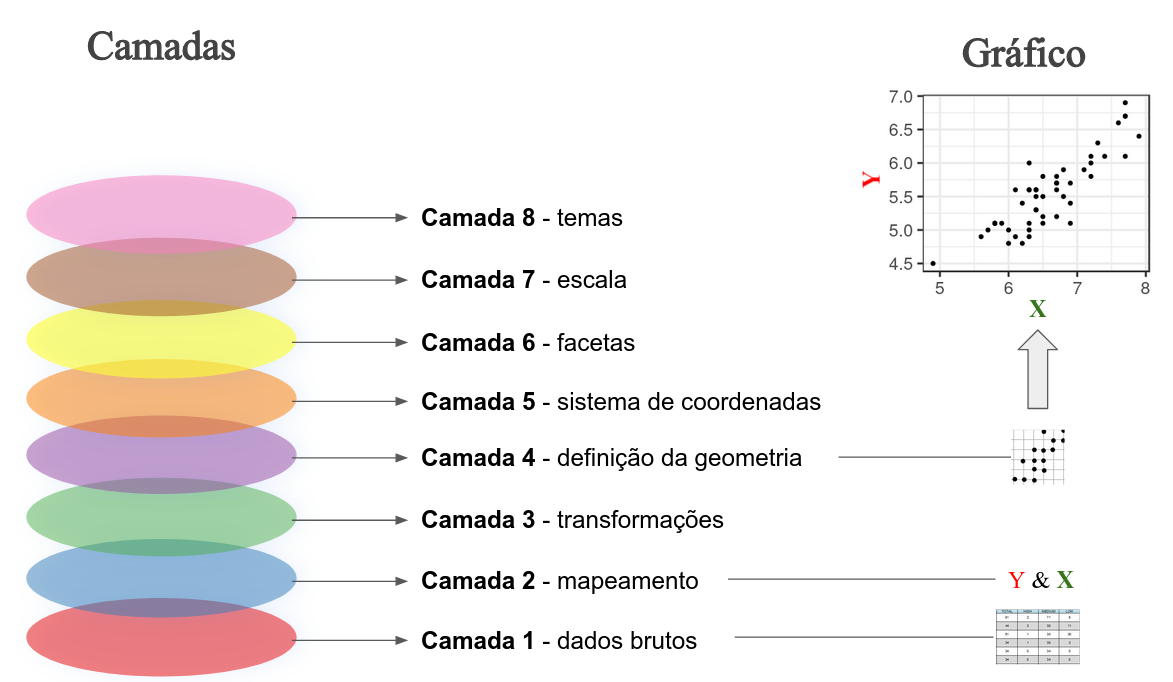
\includegraphics[width=0.7\linewidth]{img/cap06_fig01} 

}

\caption{Esquema gráfico ilustrando as camadas que definem a strutura de organização aditiva da gramática dos gráficos (ggplot2). No exemplo, a partir de uma banco de dados, o mapeamento de quais colunas representam o eixo Y e X e de um atributo gráfico (pontos) é possível construir um gráfico de dispersão que ilustra a relação quantitativa entre a variável Y e X.}\label{fig:fig-camadas}
\end{figure}

Em resumo, o mapeamento gráfico do ggplot2 segue a seguinte estrutura:

\begin{verbatim}
ggplot(data = <DATA>) + 
<GEOM_FUNCTION>(
       mapping = aes(<MAPPINGS>),
       stat = <STAT>, 
       position = <POSITION>
) +
<COORDINATE_FUNCTION> +
<FACET_FUNCTION> +
<SCALE_FUNCTION> +
<THEME_FUNCTION>
\end{verbatim}

\hypertarget{tipos-de-gruxe1ficos}{%
\section{4. Tipos de gráficos}\label{tipos-de-gruxe1ficos}}

Nesta seção, listamos os principais gráficos, e uma descrição de quantas colunas e o tipo de variável que eles representam.

\begin{itemize}
\tightlist
\item
  \textbf{Histograma (do inglês \emph{histogram})}: distribuição de frequência de uma coluna para dados contínuos (cores diferentes podem representar espécies, populações ou grupos distintos)
\item
  \textbf{Gráfico de densidade (\emph{density plot})}: distribuição da densidade de uma coluna para dados contínuos (assim como no histograma, cores diferentes podem ser utilizadas para representar espécies, populações ou grupos distintos)
\item
  \textbf{Gráfico de dispersão (\emph{scatter plot}) e gráfico de linha}: relação entre valores de duas colunas para dados contínuos (X e Y)
\item
  \textbf{Diagrama de pontos (\emph{dot plot})}: distribuição da quantidade de valores agrupados de uma coluna para dados contínuos
\item
  \textbf{Gráfico de setores (\emph{pie chart} e \emph{donut chart})}: representação da quantidade de valores de uma coluna para dados categóricos, geralmente em proporção ou porcentagem
\item
  \textbf{Gráfico de barras (\emph{bar plot})}: representação da quantidade de valores de uma ou mais colunas para dados categóricos
\item
  \textbf{Gráfico de caixa (\emph{box plot} e \emph{violin plot})}: distribuição de valores contínuos de uma coluna (Y) para dois ou mais fatores categóricos de outra coluna (X) no formato de caixas e também no formato de ``violinos'' (considerando a variação)
\item
  \textbf{Gráfico pareado (\emph{pairs plot})}: relação entre valores de duas colunas para dados contínuos (X e Y), para colunas par a par
\end{itemize}

Para facilitar a compreensão das regras da gramática dos dados, cada tipo de gráfico segue a mesma estrutura de organização, que respeita as camadas de informação descritas anteriormente. O leitor vai perceber, portanto, que algumas camadas não são necessárias dependendo do tipo de gráfico e do conjunto de dados que pretende analisar. Nos exemplos, a \emph{versão padrão} se refere à representação determinada no ``default'' da função. Deste modo, somente informamos as variáveis que serão utilizadas dentro de cada camada e a forma geométrica (i.e., tipo de gráfico) desejada. Porém, para cada tipo gráfico apresentamos funções e argumentos para ajustes finos e personalizados.

\hypertarget{histograma-histogram}{%
\subsection{\texorpdfstring{4.1. Histograma (\emph{histogram})}{4.1. Histograma (histogram)}}\label{histograma-histogram}}

O histograma é um gráfico extremamente popular e bastante útil para visualizar a distribuição de variáveis contínuas. É bem provável que você já tenha visto um histograma quando aprendeu pela primeira vez a famosa \emph{distribuição normal}.

\begin{Shaded}
\begin{Highlighting}[]
\CommentTok{\# histograma de uma variavel continua}

\NormalTok{dist\_normal }\OtherTok{\textless{}{-}} \FunctionTok{data.frame}\NormalTok{(}\AttributeTok{x =} \FunctionTok{rnorm}\NormalTok{(}\DecValTok{50000}\NormalTok{, }\AttributeTok{mean =} \DecValTok{100}\NormalTok{, }\AttributeTok{sd =} \DecValTok{5}\NormalTok{))}
\FunctionTok{ggplot}\NormalTok{(}\AttributeTok{data =}\NormalTok{ dist\_normal, }
       \FunctionTok{aes}\NormalTok{(}\AttributeTok{x =}\NormalTok{ x)) }\SpecialCharTok{+}
  \FunctionTok{geom\_histogram}\NormalTok{()}
\end{Highlighting}
\end{Shaded}

\begin{center}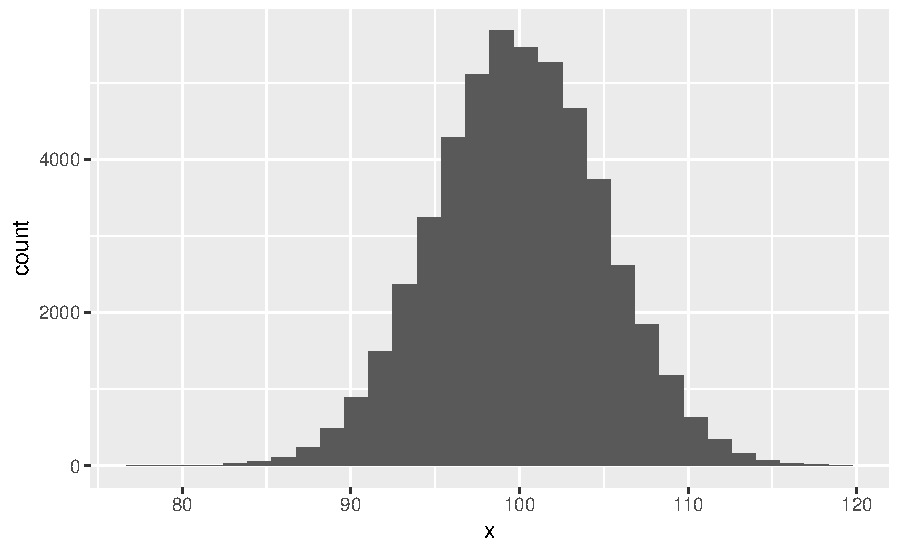
\includegraphics[width=0.7\linewidth]{livro_files/figure-latex/unnamed-chunk-181-1} \end{center}

Neste histograma é possível entender que a maioria dos valores da variável \texttt{x} no data.frame \texttt{dist\_normal} estão próximos ao valor da média, i.e., 100. Em ecologia, os histogramas são utilizados para visualizar, por exemplo, a variação morfológica entre espécies (subespécies, gênero, famílias, etc.), variação de parâmetros populacionais entre diferentes espécies ou dentro da mesma espécies em diferentes localidades.

\hypertarget{versuxe3o-padruxe3o}{%
\subsubsection{4.1.1. Versão padrão}\label{versuxe3o-padruxe3o}}

Vamos utilizar o conjunto de dados \emph{palmerpenguins} para construir um histograma da distribuição da variável \textbf{flipper\_length\_mm} com a função \texttt{geom\_hitogram()}. Esta função utiliza uma variável contínua no eixo x e a frequência de cada categoria no eixo y. O gráfico a seguir representa a frequência de uma variável (neste caso, a medida de todos os pinguins, independente da espécie).

\begin{Shaded}
\begin{Highlighting}[]

\FunctionTok{ggplot}\NormalTok{(}\AttributeTok{data =}\NormalTok{ penguins, }
       \FunctionTok{aes}\NormalTok{(}\AttributeTok{x =}\NormalTok{ flipper\_length\_mm)) }\SpecialCharTok{+}
  \FunctionTok{geom\_histogram}\NormalTok{()}
\end{Highlighting}
\end{Shaded}

\begin{center}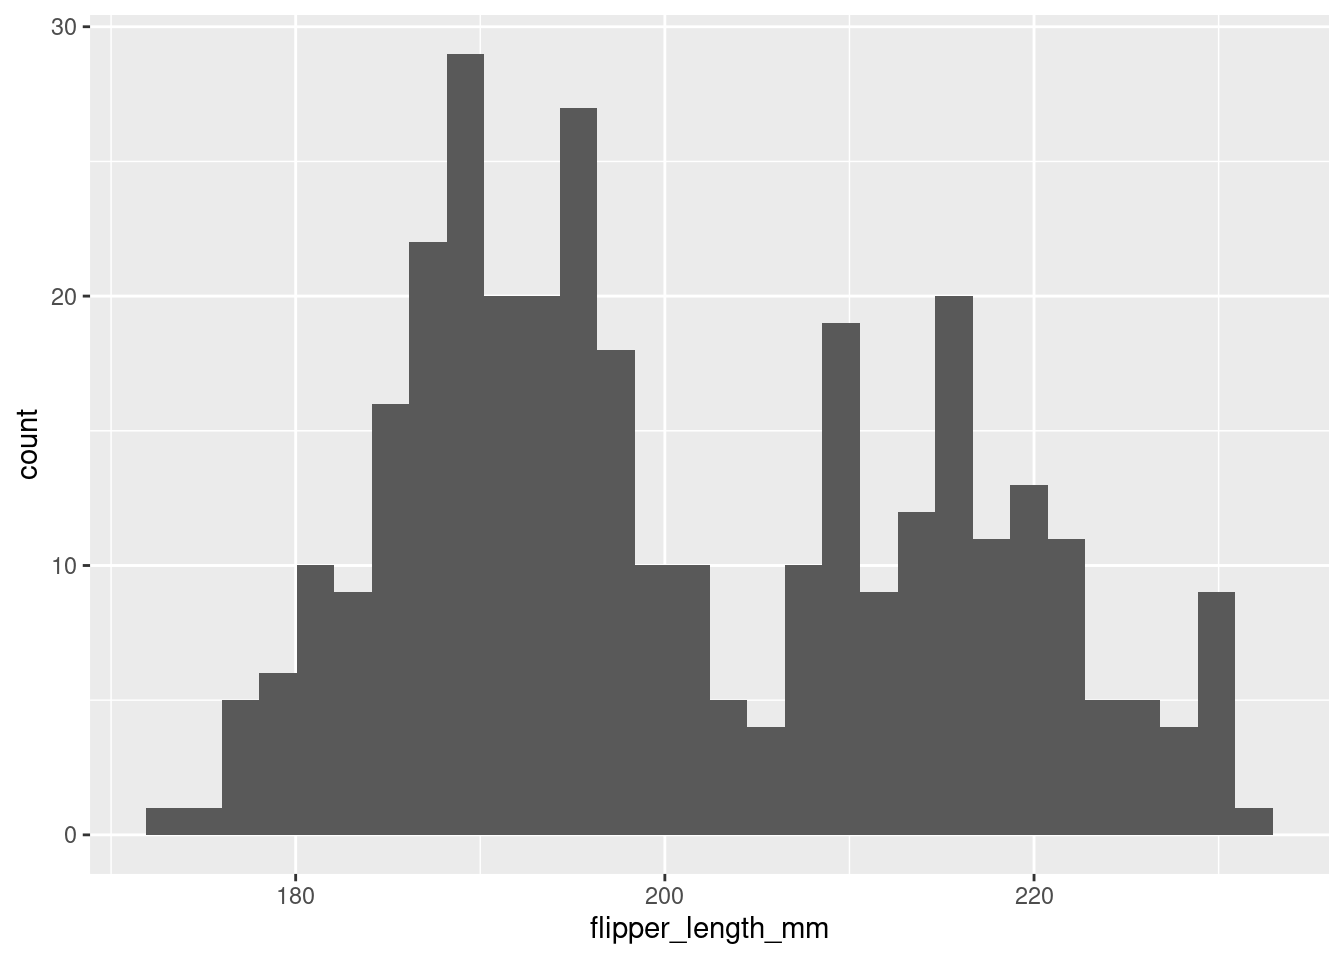
\includegraphics[width=0.7\linewidth]{livro_files/figure-latex/unnamed-chunk-182-1} \end{center}

\hypertarget{definindo-o-nuxfamero-de-classes}{%
\subsubsection{4.1.2. Definindo o número de classes}\label{definindo-o-nuxfamero-de-classes}}

Vamos utilizar o \textbf{argumento} \texttt{bins} para definir em quantas classes a variável \textbf{x} deve ser dividida.

\begin{Shaded}
\begin{Highlighting}[]

\CommentTok{\# histograma com 10 classes}
\FunctionTok{ggplot}\NormalTok{(}\AttributeTok{data =}\NormalTok{ penguins, }
       \FunctionTok{aes}\NormalTok{(}\AttributeTok{x =}\NormalTok{ flipper\_length\_mm)) }\SpecialCharTok{+}
  \FunctionTok{geom\_histogram}\NormalTok{(}\AttributeTok{bins =} \DecValTok{10}\NormalTok{) }\SpecialCharTok{+}
  \FunctionTok{labs}\NormalTok{(}\AttributeTok{title =} \StringTok{"10 classes"}\NormalTok{)}

\CommentTok{\# histograma com 30 classes}
\FunctionTok{ggplot}\NormalTok{(}\AttributeTok{data =}\NormalTok{ penguins, }\FunctionTok{aes}\NormalTok{(}\AttributeTok{x =}\NormalTok{ flipper\_length\_mm)) }\SpecialCharTok{+}
  \FunctionTok{geom\_histogram}\NormalTok{(}\AttributeTok{bins =} \DecValTok{30}\NormalTok{) }\SpecialCharTok{+}
  \FunctionTok{labs}\NormalTok{(}\AttributeTok{title =} \StringTok{"30 classes"}\NormalTok{)}
\end{Highlighting}
\end{Shaded}

\begin{center}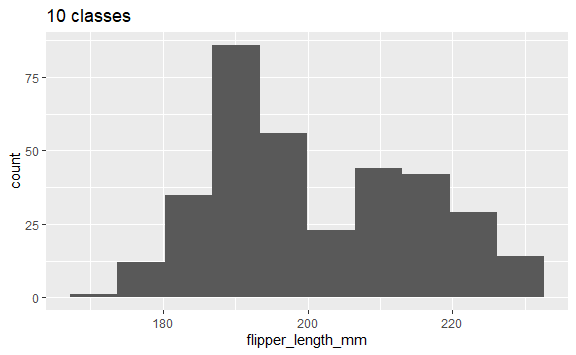
\includegraphics[width=0.5\linewidth]{livro_files/figure-latex/unnamed-chunk-183-1} 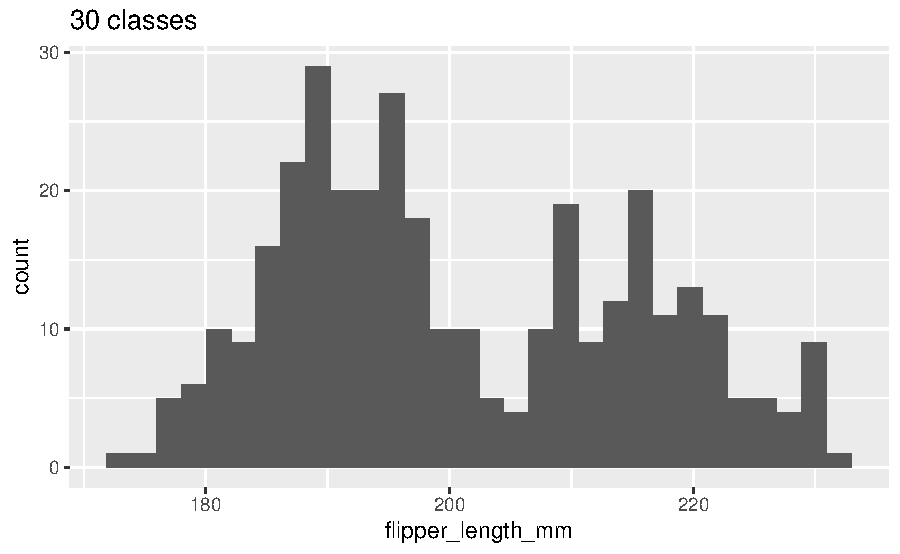
\includegraphics[width=0.5\linewidth]{livro_files/figure-latex/unnamed-chunk-183-2} \end{center}

\hypertarget{comparando-muxfaltiplas-categorias}{%
\subsubsection{4.1.3. Comparando múltiplas categorias}\label{comparando-muxfaltiplas-categorias}}

Se quisermos comparar a distribuição de uma variável contínua entre diferentes categorias, podemos utilizar o argumento \texttt{fill} para colorir o gráfico. No exemplo abaixo, utilizamos cores diferentes para ilustrar a distribuição da variável x entre espécies diferentes (fill = species).

\begin{Shaded}
\begin{Highlighting}[]
\CommentTok{\# histograma com cores para diferentes categorias com sobreposicao}
\FunctionTok{ggplot}\NormalTok{(}\AttributeTok{data =}\NormalTok{ penguins, }
       \FunctionTok{aes}\NormalTok{(}\AttributeTok{x =}\NormalTok{ flipper\_length\_mm, }\AttributeTok{fill =}\NormalTok{ species)) }\SpecialCharTok{+}
  \FunctionTok{geom\_histogram}\NormalTok{(}\AttributeTok{alpha =}\NormalTok{ .}\DecValTok{5}\NormalTok{) }\SpecialCharTok{+}
  \FunctionTok{ggtitle}\NormalTok{(}\StringTok{"Com sobreposiçao"}\NormalTok{)}

\CommentTok{\# Histograma com cores para diferentes categorias sem sobreposição}
\FunctionTok{ggplot}\NormalTok{(}\AttributeTok{data =}\NormalTok{ penguins, }\FunctionTok{aes}\NormalTok{(}\AttributeTok{x =}\NormalTok{ flipper\_length\_mm, }\AttributeTok{fill =}\NormalTok{ species)) }\SpecialCharTok{+}
  \FunctionTok{geom\_histogram}\NormalTok{(}\AttributeTok{position =} \StringTok{"dodge"}\NormalTok{) }\SpecialCharTok{+}
  \FunctionTok{ggtitle}\NormalTok{(}\StringTok{"Sem sobreposiçao"}\NormalTok{)}
\end{Highlighting}
\end{Shaded}

\begin{center}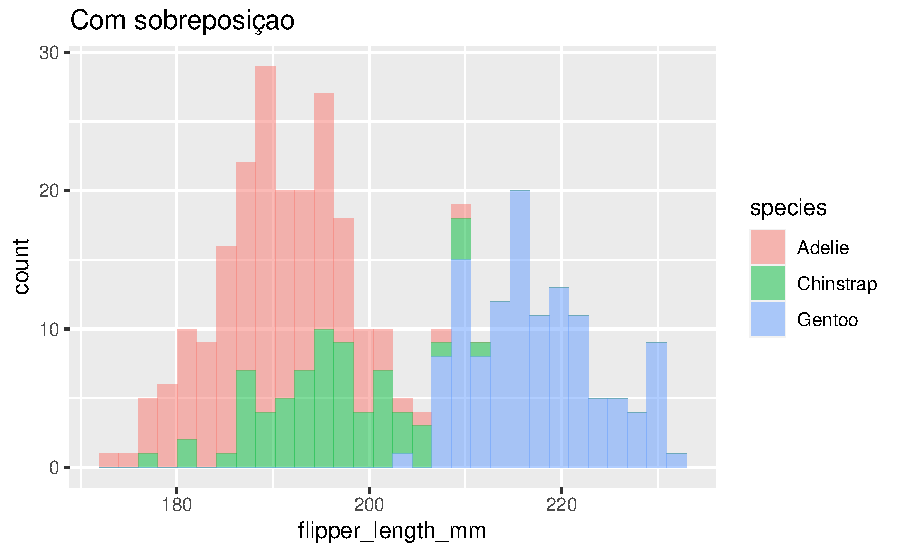
\includegraphics[width=0.5\linewidth]{livro_files/figure-latex/unnamed-chunk-184-1} 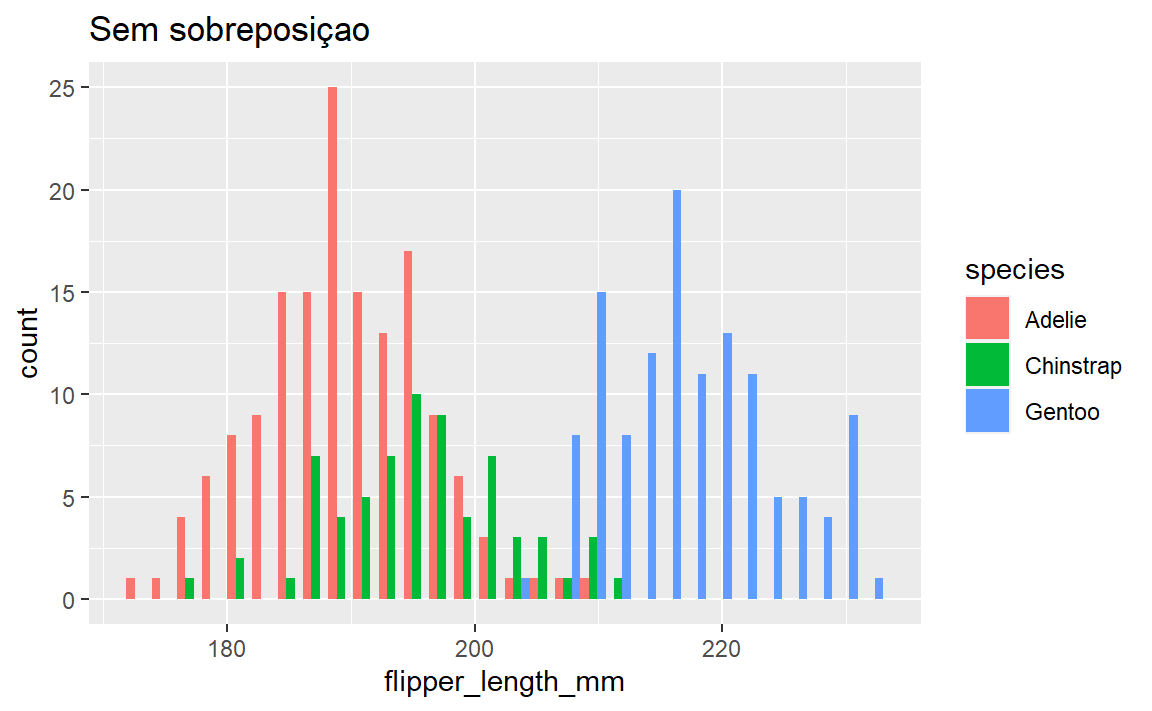
\includegraphics[width=0.5\linewidth]{livro_files/figure-latex/unnamed-chunk-184-2} \end{center}

\hypertarget{ajustes-finos-versuxe3o-personalizada}{%
\subsubsection{4.1.4. Ajustes finos (versão personalizada)}\label{ajustes-finos-versuxe3o-personalizada}}

\begin{Shaded}
\begin{Highlighting}[]
\CommentTok{\# Histogram example: flipper length by species}

\NormalTok{penguins }\SpecialCharTok{\%\textgreater{}\%} 
\FunctionTok{ggplot}\NormalTok{(}\FunctionTok{aes}\NormalTok{(}\AttributeTok{x =}\NormalTok{ flipper\_length\_mm, }\AttributeTok{fill =}\NormalTok{ species)) }\SpecialCharTok{+}
  \FunctionTok{geom\_histogram}\NormalTok{(}\AttributeTok{alpha =}\NormalTok{ .}\DecValTok{5}\NormalTok{, }\AttributeTok{position =} \StringTok{"identity"}\NormalTok{) }\SpecialCharTok{+}
  \FunctionTok{scale\_fill\_manual}\NormalTok{(}\AttributeTok{values =} \FunctionTok{c}\NormalTok{(}\StringTok{"darkorange"}\NormalTok{, }\StringTok{"darkorchid"}\NormalTok{, }\StringTok{"cyan4"}\NormalTok{)) }\SpecialCharTok{+}
  \FunctionTok{theme\_bw}\NormalTok{(}\AttributeTok{base\_size =} \DecValTok{16}\NormalTok{) }\SpecialCharTok{+}
  \FunctionTok{labs}\NormalTok{(}\AttributeTok{x =} \StringTok{"Comprimento da nadadeira (mm)"}\NormalTok{, }
       \AttributeTok{y =} \StringTok{"Frequência (\%)"}\NormalTok{, }
       \AttributeTok{fill =} \StringTok{"Espécies"}\NormalTok{)}
\end{Highlighting}
\end{Shaded}

\begin{center}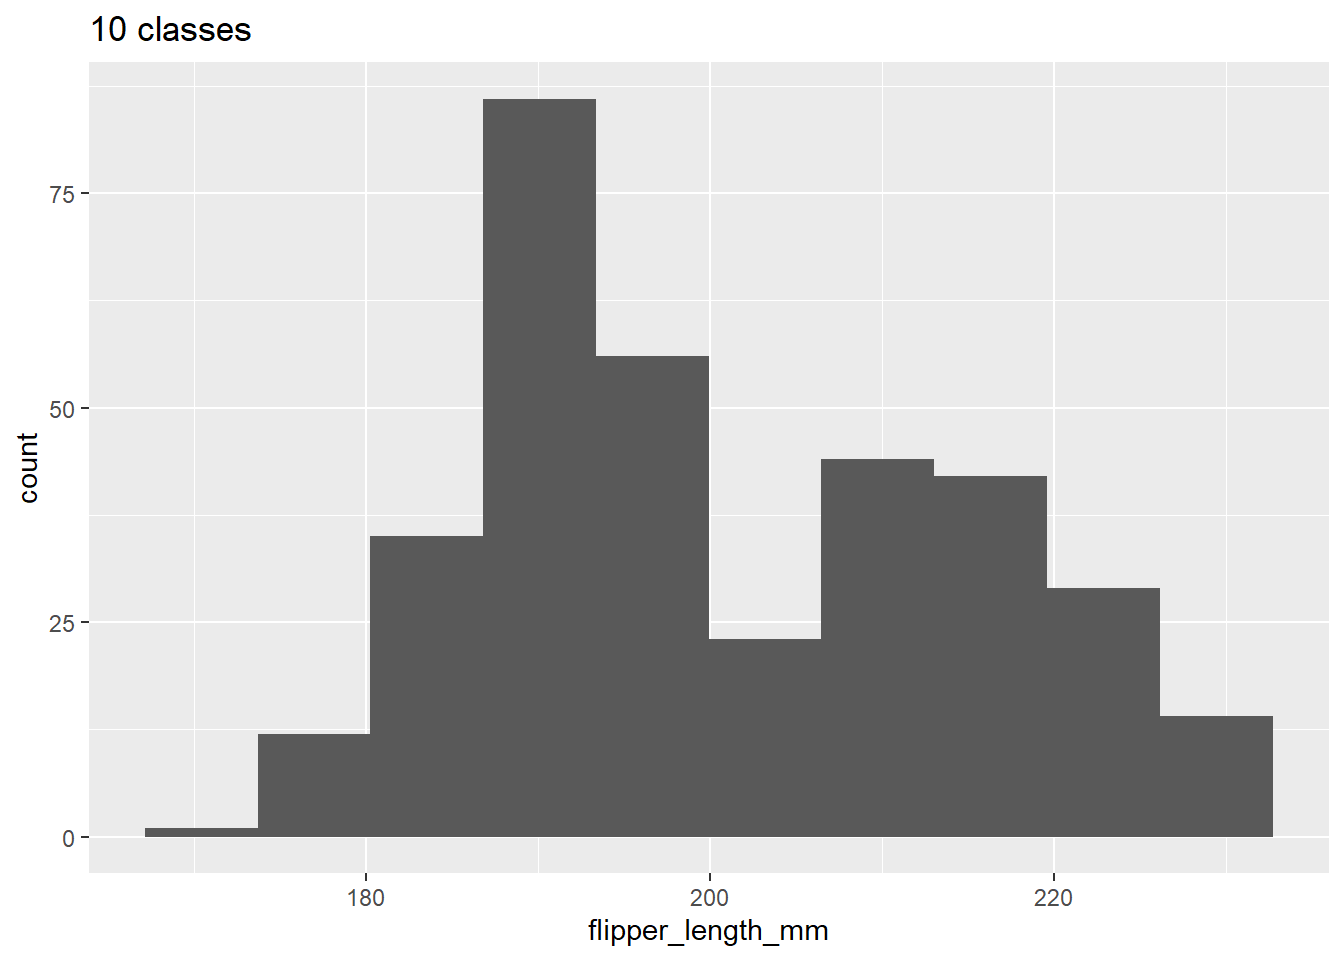
\includegraphics[width=0.7\linewidth]{livro_files/figure-latex/unnamed-chunk-185-1} \end{center}

\hypertarget{principais-camadas-utilizadas-na-funuxe7uxe3o-geom_histogram}{%
\subsubsection{\texorpdfstring{4.1.5. Principais camadas utilizadas na função \texttt{geom\_histogram()}}{4.1.5. Principais camadas utilizadas na função geom\_histogram()}}\label{principais-camadas-utilizadas-na-funuxe7uxe3o-geom_histogram}}

\begin{itemize}
\item
  \texttt{aes()}:

  \begin{itemize}
  \item
    Eixo X: variável contínua (\emph{flipper\_length\_mm})
  \item
    Preenchimento (\emph{fill}): variável categórica (\emph{species}) que define as cores tendo como base o número de níveis dentro desta categoria
  \end{itemize}
\item
  \texttt{geom():} \texttt{geom\_histogram()}

  \begin{itemize}
  \item
    Transparência dos pontos (\texttt{alpha}): 0,5 (varia de 0, trasparência máxima, a 1, sem trasparência)
  \item
    Posição das barras: o argumento \texttt{position} define se as barras devem ser inseridas de maneira sobreposta (\texttt{position\ =\ "identity"}) ou não (\texttt{position\ =\ "dodge"})
  \end{itemize}
\item
  \texttt{scale()}:\texttt{scale\_fill\_manual()} para definir manualmente as cores de preferência do usuário
\item
  \texttt{theme()}: \texttt{theme\_bw()}para selecionar o tema com fundo branco e \texttt{labs()} para personalizar o títulos dos eixos X e Y.
\end{itemize}

\hypertarget{gruxe1fico-de-densidade-density-plot}{%
\subsection{\texorpdfstring{4.2 Gráfico de densidade (\emph{density plot})}{4.2 Gráfico de densidade (density plot)}}\label{gruxe1fico-de-densidade-density-plot}}

Nesta seção iremos aprender a criar um \href{https://datavizcatalogue.com/methods/density_plot.html}{gráfico de densidade} no R utilizando o ggplot2. Assim como o histograma, o \textbf{gráfico de densidade} é utilizado para visualizar a distribuição de uma variável contínua em intervalos. Esse gráfico é uma variação do Histograma (ver seção \ref{hist}) que utiliza \href{https://en.wikipedia.org/wiki/Kernel_smoother}{Kernel Smoother} e, além de ser muito útil para visualizar distribuições, pode ser usado para testar várias hipóteses ecológicas, como descrito no \textbf{Capítulo 14 (Diversidade Funcional)}.

\hypertarget{versuxe3o-padruxe3o-1}{%
\subsubsection{4.2.1.Versão padrão}\label{versuxe3o-padruxe3o-1}}

Vamos utilizar o conjunto de dados \emph{palmerpenguins}, para plotar a distribuição da variável \textbf{flipper\_length\_mm} em um Gráfico de densidade. Utilizaremos a função \texttt{geom\_density()} para plotar uma variável no eixo x.

\begin{Shaded}
\begin{Highlighting}[]

\FunctionTok{ggplot}\NormalTok{(}\AttributeTok{data =}\NormalTok{ penguins, }
       \FunctionTok{aes}\NormalTok{(}\AttributeTok{x =}\NormalTok{ flipper\_length\_mm)) }\SpecialCharTok{+}
  \FunctionTok{geom\_density}\NormalTok{()}
\end{Highlighting}
\end{Shaded}

\begin{center}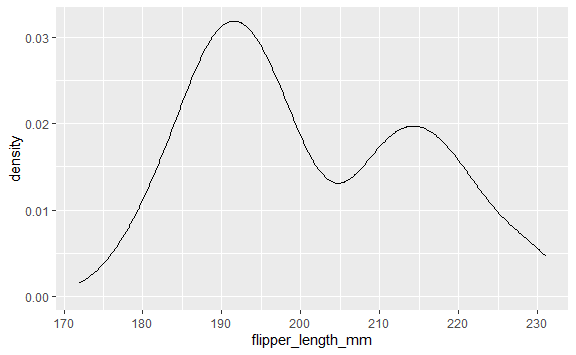
\includegraphics[width=0.7\linewidth]{livro_files/figure-latex/unnamed-chunk-186-1} \end{center}

Além da versão de densidade em linha, é possível utilizar o argumento \texttt{fill} para definir a cor de preenchimento do gráfico e o argumento \texttt{alpha} para definir a transparência do preenchimento. Utilizamos ainda o argumento \texttt{color} para definir a cor da linha.

\begin{Shaded}
\begin{Highlighting}[]

\CommentTok{\# Argumento fill}
\FunctionTok{ggplot}\NormalTok{(}\AttributeTok{data =}\NormalTok{ penguins, }
       \FunctionTok{aes}\NormalTok{(}\AttributeTok{x =}\NormalTok{ flipper\_length\_mm)) }\SpecialCharTok{+}
  \FunctionTok{geom\_density}\NormalTok{(}\AttributeTok{fill =} \StringTok{"tomato"}\NormalTok{)}

\CommentTok{\# Argumento fill, color e alpha}
\FunctionTok{ggplot}\NormalTok{(}\AttributeTok{data =}\NormalTok{ penguins, }
       \FunctionTok{aes}\NormalTok{(}\AttributeTok{x =}\NormalTok{ flipper\_length\_mm)) }\SpecialCharTok{+}
  \FunctionTok{geom\_density}\NormalTok{(}\AttributeTok{fill =} \StringTok{"steelblue"}\NormalTok{, }
               \AttributeTok{color =} \StringTok{"black"}\NormalTok{, }
               \AttributeTok{alpha =}\NormalTok{ .}\DecValTok{5}\NormalTok{)}
\end{Highlighting}
\end{Shaded}

\begin{center}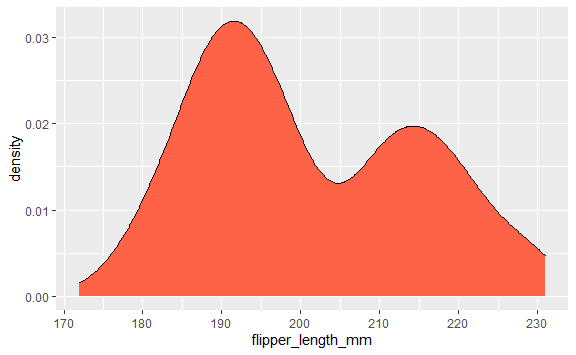
\includegraphics[width=0.5\linewidth]{livro_files/figure-latex/unnamed-chunk-187-1} 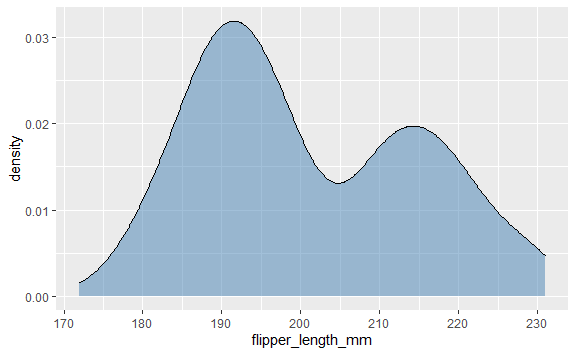
\includegraphics[width=0.5\linewidth]{livro_files/figure-latex/unnamed-chunk-187-2} \end{center}

\hypertarget{comparando-muxfaltiplas-categorias-1}{%
\subsubsection{4.2.2. Comparando múltiplas categorias}\label{comparando-muxfaltiplas-categorias-1}}

Em algumas situações, queremos comparar a distribuição de uma variável contínua entre diferentes categorias. Dessa forma, podemos utilizar o argumento \texttt{fill} para colorir o gráfico. No exemplo abaixo, utilizamos cores diferentes para ilustrar a distribuição da variável x entre espécies diferentes (fill = species).

\begin{Shaded}
\begin{Highlighting}[]

\CommentTok{\# O argumento fill preenche cada nível da coluna "species" (sem transparência: alpha = 1)}

\FunctionTok{ggplot}\NormalTok{(}\AttributeTok{data =}\NormalTok{ penguins, }
       \FunctionTok{aes}\NormalTok{(}\AttributeTok{x =}\NormalTok{ flipper\_length\_mm, }\AttributeTok{fill =}\NormalTok{ species)) }\SpecialCharTok{+}
  \FunctionTok{geom\_density}\NormalTok{() }\SpecialCharTok{+}
  \FunctionTok{labs}\NormalTok{(}\AttributeTok{title =} \StringTok{"Sem transparência"}\NormalTok{)}

\CommentTok{\# Gráfico de densidade com cores para diferentes categorias com sobreposicao}
\FunctionTok{ggplot}\NormalTok{(}\AttributeTok{data =}\NormalTok{ penguins, }
       \FunctionTok{aes}\NormalTok{(}\AttributeTok{x =}\NormalTok{ flipper\_length\_mm, }\AttributeTok{fill =}\NormalTok{ species)) }\SpecialCharTok{+}
  \FunctionTok{geom\_density}\NormalTok{(}\AttributeTok{alpha =}\NormalTok{ .}\DecValTok{5}\NormalTok{) }\SpecialCharTok{+}
  \FunctionTok{labs}\NormalTok{(}\AttributeTok{title =} \StringTok{"Com transparência"}\NormalTok{)}
\end{Highlighting}
\end{Shaded}

\begin{center}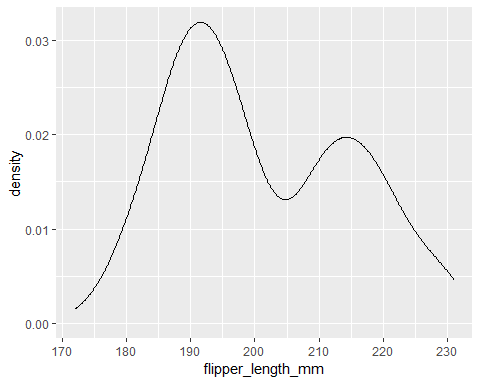
\includegraphics[width=0.5\linewidth]{livro_files/figure-latex/unnamed-chunk-188-1} 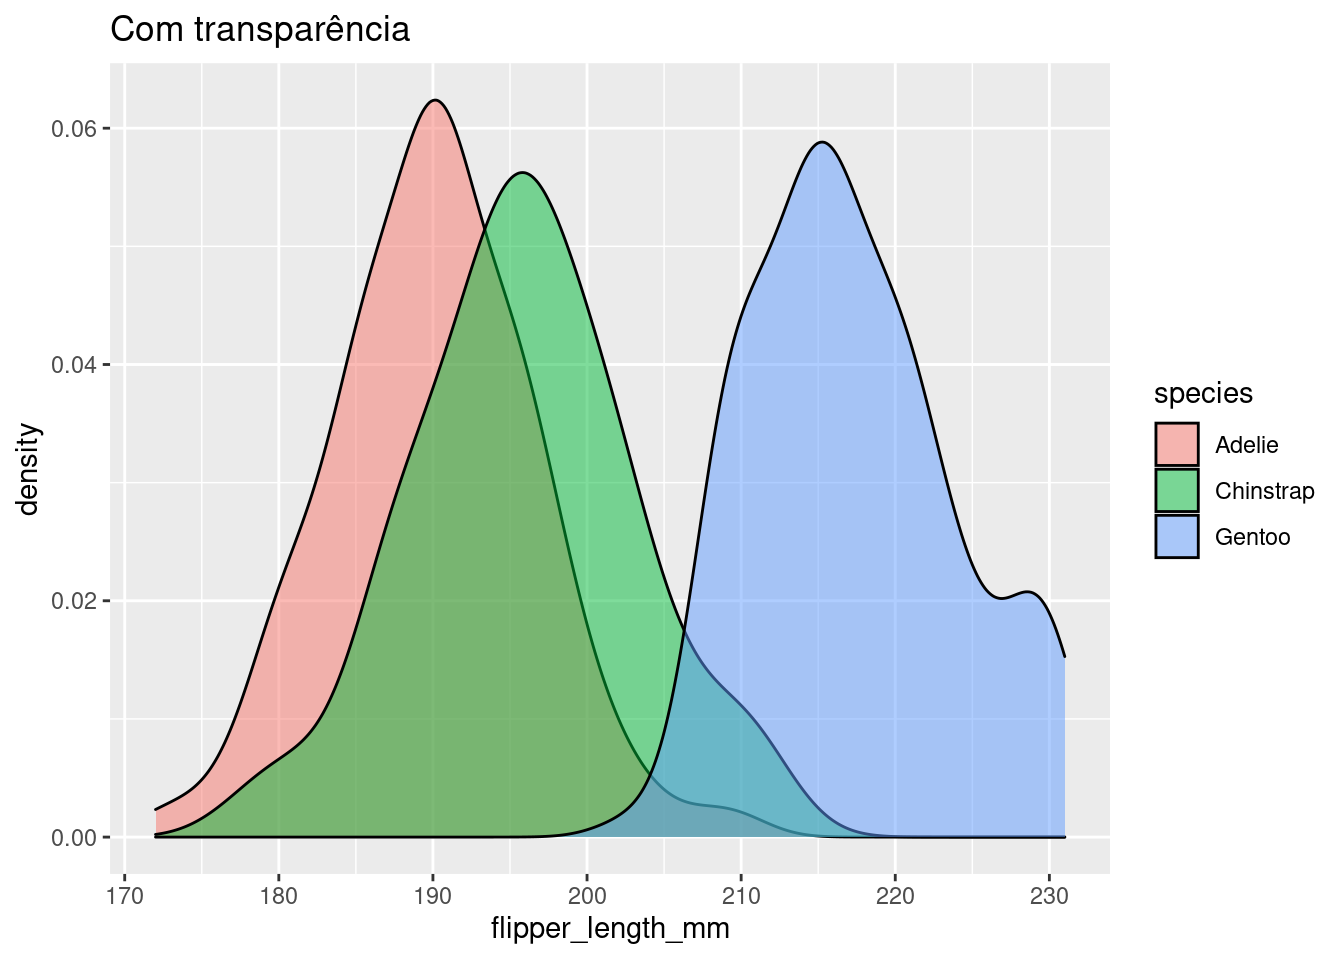
\includegraphics[width=0.5\linewidth]{livro_files/figure-latex/unnamed-chunk-188-2} \end{center}

\hypertarget{ajustes-finos-versuxe3o-personalizada-1}{%
\subsubsection{4.2.3. Ajustes finos (versão personalizada)}\label{ajustes-finos-versuxe3o-personalizada-1}}

\begin{Shaded}
\begin{Highlighting}[]
\FunctionTok{ggplot}\NormalTok{(}\AttributeTok{data =}\NormalTok{ penguins, }
       \FunctionTok{aes}\NormalTok{(}\AttributeTok{x =}\NormalTok{ flipper\_length\_mm, }\AttributeTok{fill =}\NormalTok{ species)) }\SpecialCharTok{+}
  \FunctionTok{geom\_density}\NormalTok{(}\AttributeTok{alpha =}\NormalTok{ .}\DecValTok{5}\NormalTok{) }\SpecialCharTok{+}
  \FunctionTok{scale\_fill\_manual}\NormalTok{(}\AttributeTok{values =} \FunctionTok{c}\NormalTok{(}\StringTok{"darkorange"}\NormalTok{, }\StringTok{"darkorchid"}\NormalTok{, }\StringTok{"cyan4"}\NormalTok{)) }\SpecialCharTok{+}
  \FunctionTok{scale\_x\_continuous}\NormalTok{(}\AttributeTok{breaks =} \FunctionTok{seq}\NormalTok{(}\AttributeTok{from =} \DecValTok{160}\NormalTok{, }\AttributeTok{to =} \DecValTok{240}\NormalTok{, }\AttributeTok{by =} \DecValTok{10}\NormalTok{), }\AttributeTok{limits =} \FunctionTok{c}\NormalTok{(}\DecValTok{160}\NormalTok{, }\DecValTok{240}\NormalTok{)) }\SpecialCharTok{+}
  \FunctionTok{scale\_y\_continuous}\NormalTok{(}\AttributeTok{breaks =} \FunctionTok{seq}\NormalTok{(}\AttributeTok{from =} \DecValTok{0}\NormalTok{, }\AttributeTok{to =}\NormalTok{ .}\DecValTok{07}\NormalTok{, }\AttributeTok{by =}\NormalTok{ .}\DecValTok{01}\NormalTok{)) }\SpecialCharTok{+}
  \FunctionTok{theme\_bw}\NormalTok{(}\AttributeTok{base\_size =} \DecValTok{16}\NormalTok{) }\SpecialCharTok{+}
  \FunctionTok{labs}\NormalTok{(}\AttributeTok{x =} \StringTok{"Comprimento da nadadeira (mm)"}\NormalTok{, }\AttributeTok{y =} \StringTok{"Frequência"}\NormalTok{, }\AttributeTok{fill =} \StringTok{"Espécie"}\NormalTok{)}
\end{Highlighting}
\end{Shaded}

\begin{center}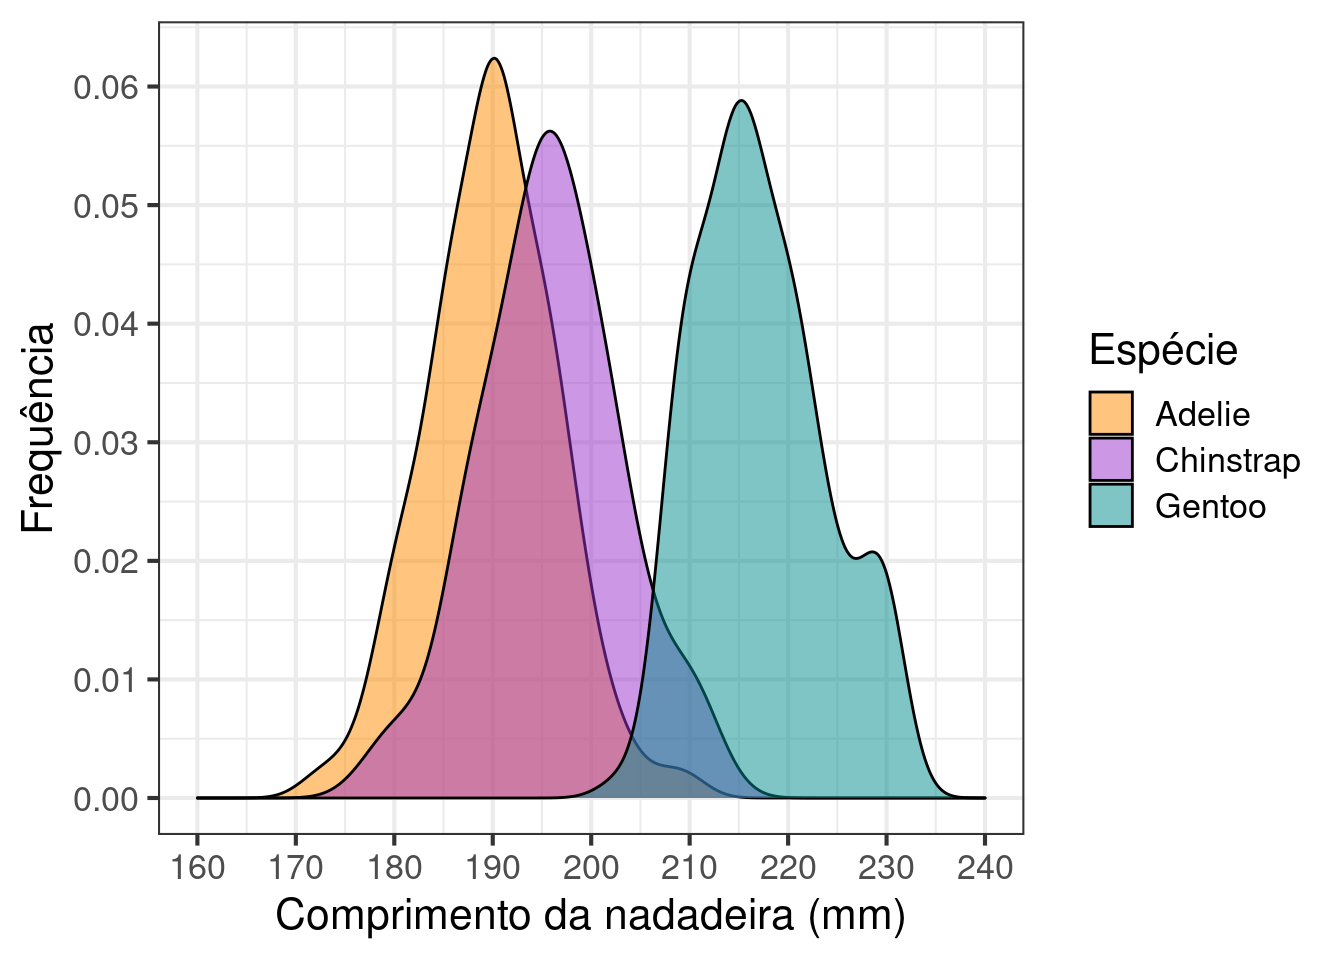
\includegraphics[width=0.7\linewidth]{livro_files/figure-latex/unnamed-chunk-189-1} \end{center}

\hypertarget{principais-camadas-utilizadas-na-funuxe7uxe3o-geom_density}{%
\subsubsection{\texorpdfstring{4.2.4. Principais camadas utilizadas na função \texttt{geom\_density()}}{4.2.4. Principais camadas utilizadas na função geom\_density()}}\label{principais-camadas-utilizadas-na-funuxe7uxe3o-geom_density}}

\begin{itemize}
\item
  \texttt{aes()}:

  \begin{itemize}
  \item
    Eixo X: variável contínua (flipper\_length\_mm)
  \item
    Preenchimento (\emph{fill}): variável categórica (\emph{species}) que define as cores tendo como base o número de níveis dentro desta categoria
  \end{itemize}
\item
  \texttt{geom():} \texttt{geom\_density()}

  \begin{itemize}
  \item
    Transparência dos pontos (\emph{alpha}): 0,5 (varia de 0, trasparência máxima, a 1, sem trasparência)
  \item
    Posição das barras: o argumento \texttt{position()} define se as barras devem ser inseridas de maneira sobreposta (\texttt{position\ =\ "identity"}) ou não (\texttt{position\ =\ "dodge"})
  \end{itemize}
\item
  \texttt{scale()}:

  \begin{itemize}
  \item
    \texttt{scale\_fill\_manual()} para definir manualmente as cores de preferência do usuário
  \item
    \texttt{scale\_x\_continuous()} e \texttt{scale\_y\_continuous()} determinam os limites (valor mínimo e máximo) para os dois eixos e, além disso, os intervalos entre os valores (\emph{breaks})
  \end{itemize}
\item
  \texttt{theme()}: \texttt{theme\_bw()}para selecionar o tema com fundo branco e \texttt{labs()} para personalizar o títulos dos eixos X e Y, e da legenda.
\end{itemize}

\hypertarget{dot}{%
\subsection{\texorpdfstring{4.3. Diagrama de pontos (\emph{dot plot})}{4.3. Diagrama de pontos (dot plot)}}\label{dot}}

Uma alternativa ao gráfico de densidade e histograma é o diagrama de pontos (\href{https://en.wikipedia.org/wiki/Dot_plot_(statistics)}{Dot plot}), apesar de ser relativamente menos usado em ecologia.

\hypertarget{versuxe3o-padruxe3o-2}{%
\subsubsection{4.3.1. Versão padrão}\label{versuxe3o-padruxe3o-2}}

Vamos utilizar o conjunto de dados palmerpenguins para visualizar a distribuição da variável flipper\_length\_mm com o diagrama de pontos com a função \texttt{geom\_dotplot()}.

\begin{Shaded}
\begin{Highlighting}[]

\FunctionTok{ggplot}\NormalTok{(}\AttributeTok{data =}\NormalTok{ penguins, }
       \FunctionTok{aes}\NormalTok{(}\AttributeTok{x =}\NormalTok{ flipper\_length\_mm)) }\SpecialCharTok{+}
  \FunctionTok{geom\_dotplot}\NormalTok{()}
\end{Highlighting}
\end{Shaded}

\begin{center}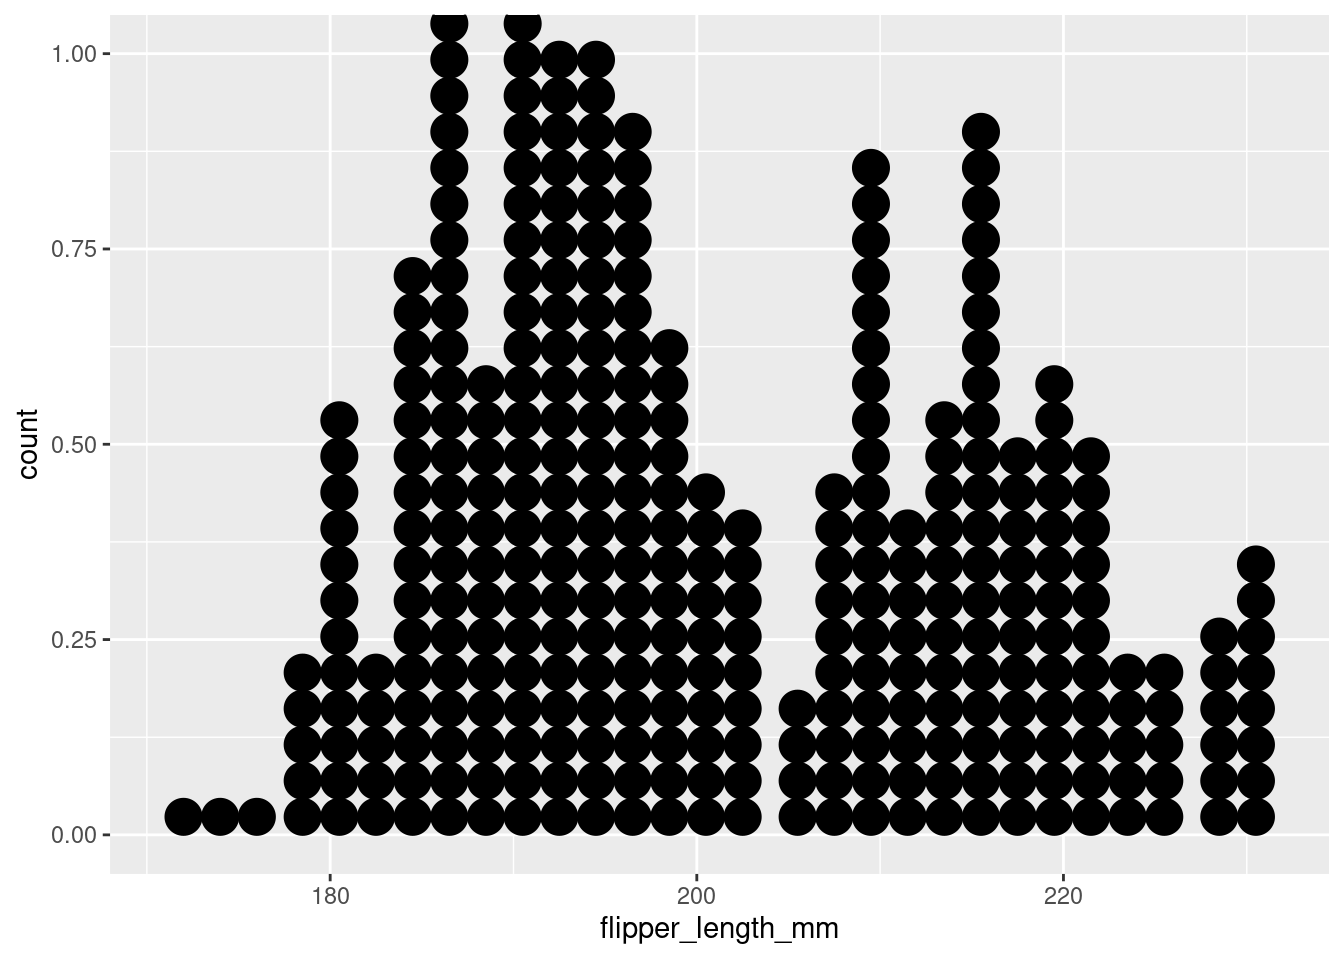
\includegraphics[width=0.7\linewidth]{livro_files/figure-latex/unnamed-chunk-190-1} \end{center}

\hypertarget{comparando-muxfaltiplas-categorias-2}{%
\subsubsection{4.3.2. Comparando múltiplas categorias}\label{comparando-muxfaltiplas-categorias-2}}

Assim como nas funções \texttt{geom\_histogram()} e \texttt{geom\_density()}, é possível comparar categorias na função \texttt{geom\_dotplot()} utilizando o argumento \texttt{fill}, bem como os argumentos \texttt{color}, \texttt{alpha} e \texttt{dotsize}.

\begin{Shaded}
\begin{Highlighting}[]
\FunctionTok{ggplot}\NormalTok{(}\AttributeTok{data =}\NormalTok{ penguins, }
       \FunctionTok{aes}\NormalTok{(}\AttributeTok{x =}\NormalTok{ flipper\_length\_mm, }\AttributeTok{fill =}\NormalTok{ species)) }\SpecialCharTok{+}
  \FunctionTok{geom\_dotplot}\NormalTok{(}\AttributeTok{dotsize=}\DecValTok{1}\NormalTok{)}

\FunctionTok{ggplot}\NormalTok{(}\AttributeTok{data =}\NormalTok{ penguins, }
       \FunctionTok{aes}\NormalTok{(}\AttributeTok{x =}\NormalTok{ flipper\_length\_mm, }\AttributeTok{fill =}\NormalTok{ species)) }\SpecialCharTok{+}
  \FunctionTok{geom\_dotplot}\NormalTok{(}\AttributeTok{dotsize=}\FloatTok{0.7}\NormalTok{, }
               \AttributeTok{color =} \StringTok{"black"}\NormalTok{, }
               \AttributeTok{alpha =} \FloatTok{0.5}\NormalTok{)}
\end{Highlighting}
\end{Shaded}

\begin{center}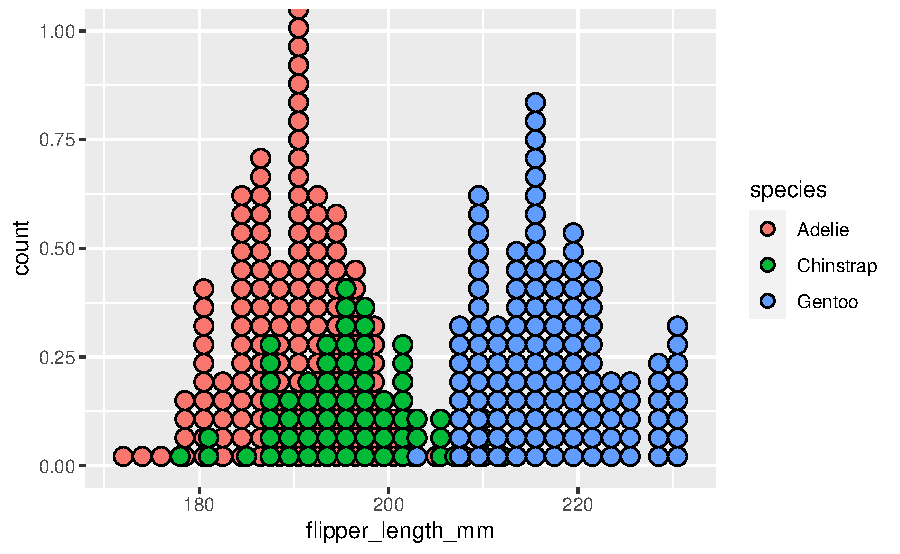
\includegraphics[width=0.5\linewidth]{livro_files/figure-latex/unnamed-chunk-191-1} 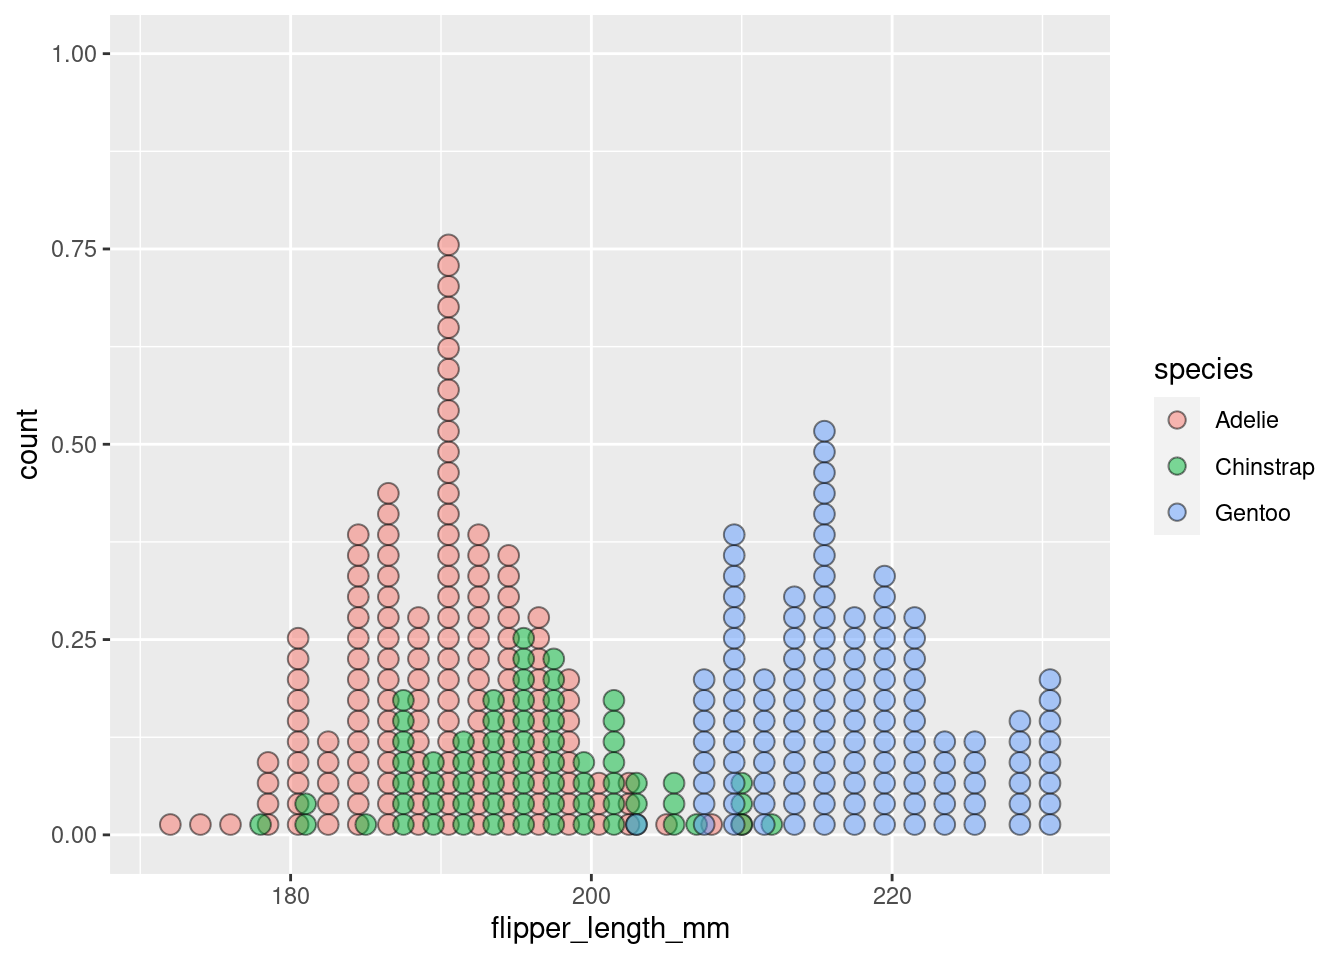
\includegraphics[width=0.5\linewidth]{livro_files/figure-latex/unnamed-chunk-191-2} \end{center}

\hypertarget{ajustes-finos-versuxe3o-personalizada-2}{%
\subsubsection{4.3.3. Ajustes finos (versão personalizada)}\label{ajustes-finos-versuxe3o-personalizada-2}}

\begin{Shaded}
\begin{Highlighting}[]
\FunctionTok{ggplot}\NormalTok{(}\AttributeTok{data =}\NormalTok{ penguins, }
       \FunctionTok{aes}\NormalTok{(}\AttributeTok{x =}\NormalTok{ flipper\_length\_mm, }\AttributeTok{fill =}\NormalTok{ species)) }\SpecialCharTok{+}
  \FunctionTok{geom\_dotplot}\NormalTok{(}\AttributeTok{color =} \StringTok{"black"}\NormalTok{, }
               \AttributeTok{alpha =}\NormalTok{ .}\DecValTok{7}\NormalTok{) }\SpecialCharTok{+}
  \FunctionTok{theme\_bw}\NormalTok{(}\AttributeTok{base\_size =} \DecValTok{16}\NormalTok{) }\SpecialCharTok{+}
  \FunctionTok{scale\_fill\_manual}\NormalTok{(}\AttributeTok{values =} \FunctionTok{c}\NormalTok{(}\StringTok{"darkorange"}\NormalTok{, }\StringTok{"darkorchid"}\NormalTok{, }\StringTok{"cyan4"}\NormalTok{)) }\SpecialCharTok{+}
  \FunctionTok{scale\_x\_continuous}\NormalTok{(}\AttributeTok{breaks =} \FunctionTok{seq}\NormalTok{(}\AttributeTok{from =} \DecValTok{170}\NormalTok{, }\AttributeTok{to =} \DecValTok{240}\NormalTok{, }\AttributeTok{by =} \DecValTok{10}\NormalTok{), }\AttributeTok{limits =} \FunctionTok{c}\NormalTok{(}\DecValTok{170}\NormalTok{, }\DecValTok{240}\NormalTok{)) }\SpecialCharTok{+}
  \FunctionTok{scale\_y\_continuous}\NormalTok{(}\AttributeTok{breaks =} \FunctionTok{seq}\NormalTok{(}\AttributeTok{from =} \DecValTok{0}\NormalTok{, }\AttributeTok{to =} \FloatTok{1.4}\NormalTok{, }\AttributeTok{by =}\NormalTok{ .}\DecValTok{2}\NormalTok{), }\AttributeTok{limits =} \FunctionTok{c}\NormalTok{(}\DecValTok{0}\NormalTok{, }\FloatTok{1.4}\NormalTok{)) }\SpecialCharTok{+}
  \FunctionTok{labs}\NormalTok{(}\AttributeTok{x =} \StringTok{"Comprimento da nadadeira (mm)"}\NormalTok{, }\AttributeTok{y =} \StringTok{"Frequência"}\NormalTok{, }\AttributeTok{fill =} \StringTok{"Espécies"}\NormalTok{)}
\end{Highlighting}
\end{Shaded}

\begin{center}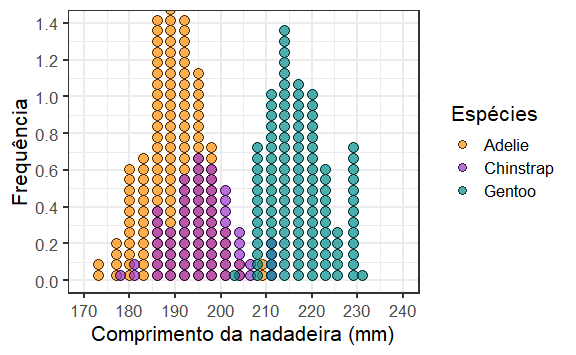
\includegraphics[width=0.7\linewidth]{livro_files/figure-latex/unnamed-chunk-192-1} \end{center}

Uma das limitações do dotplot é que a sobreposição dos pontos não permite a visualização apropriada desses valores sobrepostos entre diferentes grupos comparados.

\hypertarget{principais-camadas-utilizadas-na-funuxe7uxe3o-geom_dotplot}{%
\subsubsection{\texorpdfstring{4.3.4. Principais camadas utilizadas na função \texttt{geom\_dotplot()}}{4.3.4. Principais camadas utilizadas na função geom\_dotplot()}}\label{principais-camadas-utilizadas-na-funuxe7uxe3o-geom_dotplot}}

\begin{itemize}
\item
  \texttt{aes()}:

  \begin{itemize}
  \item
    Eixo X: variável contínua (\emph{flipper\_length\_mm})
  \item
    Preenchimento (\emph{fill}): variável categórica (\emph{species}) que define as cores tendo como base o número de níveis dentro desta categoria
  \end{itemize}
\item
  \texttt{geom():} \texttt{geom\_dotplot()}

  \begin{itemize}
  \item
    Transparência dos pontos (\texttt{alpha}): 0,5 (varia de 0, trasparência máxima, a 1, sem trasparência)
  \item
    Cor da linha do ponto (\texttt{color}): valor padrão (se não for especificado) é \emph{black}
  \item
    Tamanho dos pontos (\texttt{dotsize}): valor padrão (se não for especificado) é 1
  \item
    Posição dos pontos: o argumento \texttt{position} define se as barras devem ser inseridas de maneira sobreposta (\texttt{position\ =\ "identity"}) ou não (\texttt{position\ =\ "dodge"})
  \end{itemize}
\item
  \texttt{scale()}:

  \begin{itemize}
  \item
    \texttt{scale\_fill\_manual()} para definir manualmente as cores de preferência do usuário
  \item
    \texttt{scale\_x\_continuous()} e \texttt{scale\_y\_continuous()} determinam os limites (valor mínimo e máximo) para os dois eixos e, além disso, os intervalos entre os valores (\emph{breaks})
  \end{itemize}
\item
  \texttt{theme()}: \texttt{theme\_bw()}para selecionar o tema com fundo branco e \texttt{labs()} para personalizar o títulos dos eixos X e Y, e da legenda.
\end{itemize}

\hypertarget{bars}{%
\subsection{\texorpdfstring{4.4. Gráfico de barras (\emph{bar plot})}{4.4. Gráfico de barras (bar plot)}}\label{bars}}

O \href{https://pt.wikipedia.org/wiki/Gr\%C3\%A1fico_de_barras}{gráfico de barras} é um dos mais usados em artigos e livros da ecologia, uma vez que permite comparar valores absolutos ou médios (combinados com alguma medida de variação como desvio padrão) de uma variável continua entre diferentes níveis de uma variável categórica.

\hypertarget{versuxe3o-padruxe3o-3}{%
\subsubsection{4.4.1. Versão padrão}\label{versuxe3o-padruxe3o-3}}

O gráfico de barras utiliza retângulos para representar uma variável contínua ou a contagem de uma variável categórica, sendo que o comprimeno dos retângulos é proporcional ao valor que ele representa. Por exemplo, é possível comparar qual a quantidade de indivíduos medidos para cada espécie de pinguim.

\begin{Shaded}
\begin{Highlighting}[]
\CommentTok{\# Número de indivíduos coletados}

\NormalTok{penguins\_count }\OtherTok{\textless{}{-}}\NormalTok{ penguins }\SpecialCharTok{\%\textgreater{}\%}
\NormalTok{  dplyr}\SpecialCharTok{::}\FunctionTok{count}\NormalTok{(species)}

\CommentTok{\# grafico de barras}
\FunctionTok{ggplot}\NormalTok{(}\AttributeTok{data =}\NormalTok{ penguins\_count, }
       \FunctionTok{aes}\NormalTok{(}\AttributeTok{x =}\NormalTok{ species, }\AttributeTok{y =}\NormalTok{ n)) }\SpecialCharTok{+} 
  \FunctionTok{geom\_bar}\NormalTok{(}\AttributeTok{stat =} \StringTok{"identity"}\NormalTok{)}
\end{Highlighting}
\end{Shaded}

\begin{center}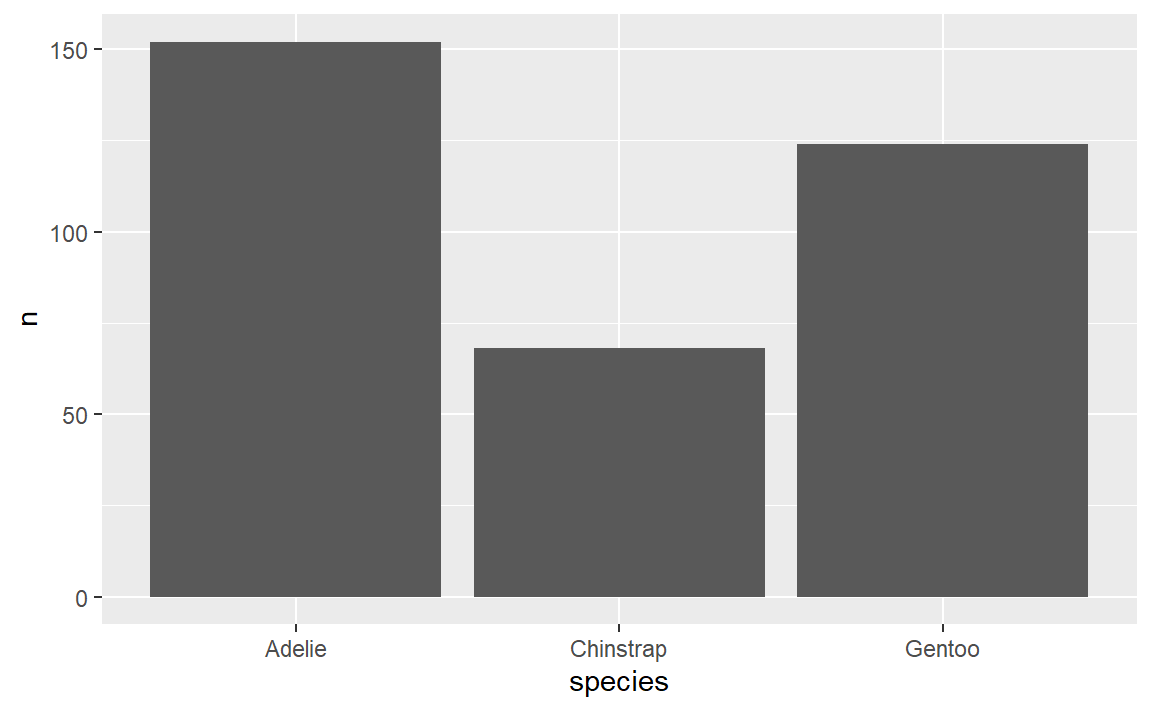
\includegraphics[width=0.7\linewidth]{livro_files/figure-latex/unnamed-chunk-193-1} \end{center}

Além disso, é possível alterar as cores (\texttt{color}) e preenchimento (\texttt{fill}) das barras, bem como sua transparência (\texttt{alpha}) e largura (\texttt{width}), como demonstrado nos próximos quatro gráficos.1

\begin{Shaded}
\begin{Highlighting}[]

\CommentTok{\# modificando preenchimento}
\FunctionTok{ggplot}\NormalTok{(}\AttributeTok{data =}\NormalTok{ penguins\_count, }
       \FunctionTok{aes}\NormalTok{(}\AttributeTok{x =}\NormalTok{ species, }\AttributeTok{y =}\NormalTok{ n)) }\SpecialCharTok{+} 
  \FunctionTok{geom\_bar}\NormalTok{(}\AttributeTok{stat =} \StringTok{"identity"}\NormalTok{, }
           \AttributeTok{fill =} \StringTok{"steelblue"}\NormalTok{)}

\CommentTok{\# Modificando cor e preenchimento}
\FunctionTok{ggplot}\NormalTok{(}\AttributeTok{data =}\NormalTok{ penguins\_count, }
       \FunctionTok{aes}\NormalTok{(}\AttributeTok{x =}\NormalTok{ species, }\AttributeTok{y =}\NormalTok{ n)) }\SpecialCharTok{+} 
  \FunctionTok{geom\_bar}\NormalTok{(}\AttributeTok{stat =} \StringTok{"identity"}\NormalTok{, }
           \AttributeTok{color =} \StringTok{"steelblue"}\NormalTok{, }
           \AttributeTok{fill =} \StringTok{"white"}\NormalTok{)}
\end{Highlighting}
\end{Shaded}

\begin{center}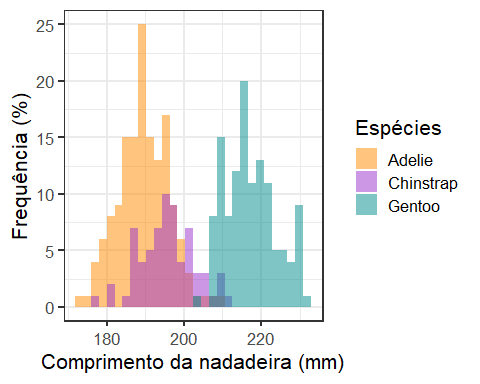
\includegraphics[width=0.5\linewidth]{livro_files/figure-latex/unnamed-chunk-194-1} 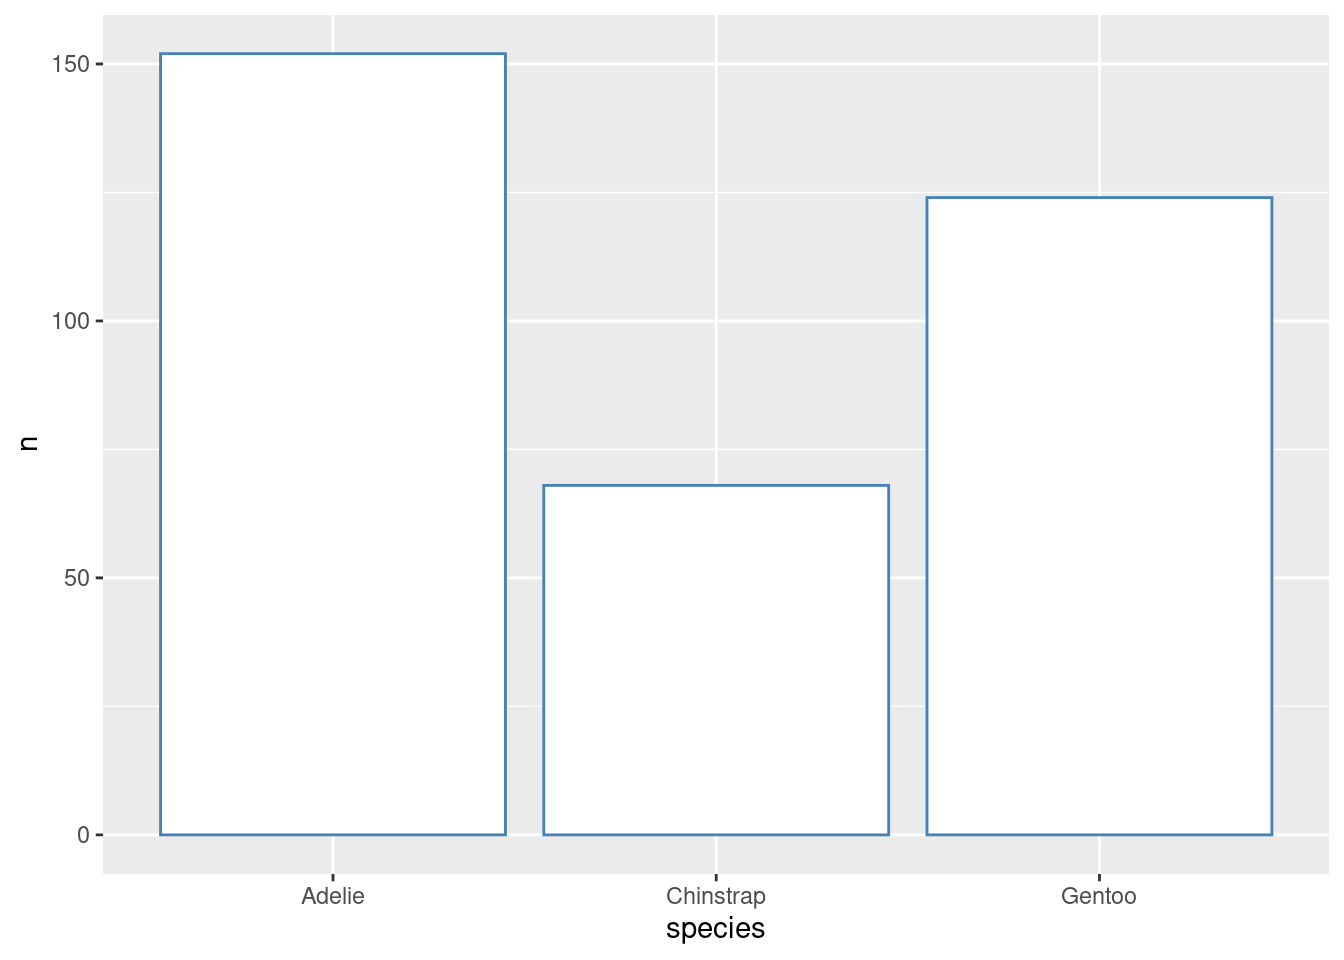
\includegraphics[width=0.5\linewidth]{livro_files/figure-latex/unnamed-chunk-194-2} \end{center}

\begin{Shaded}
\begin{Highlighting}[]

\CommentTok{\# Modificando a largura da barra = 0.75}
\FunctionTok{ggplot}\NormalTok{(}\AttributeTok{data =}\NormalTok{ penguins\_count, }
       \FunctionTok{aes}\NormalTok{(}\AttributeTok{x =}\NormalTok{ species, }\AttributeTok{y =}\NormalTok{ n)) }\SpecialCharTok{+}
  \FunctionTok{geom\_bar}\NormalTok{(}\AttributeTok{stat =} \StringTok{"identity"}\NormalTok{, }
           \AttributeTok{width =} \FloatTok{0.75}\NormalTok{) }\SpecialCharTok{+}
  \FunctionTok{labs}\NormalTok{(}\AttributeTok{title =} \StringTok{"largura = 0.75"}\NormalTok{)}

\CommentTok{\# Modificando a largura da barra = 0.25}
\FunctionTok{ggplot}\NormalTok{(}\AttributeTok{data =}\NormalTok{ penguins\_count, }
       \FunctionTok{aes}\NormalTok{(}\AttributeTok{x =}\NormalTok{ species, }\AttributeTok{y =}\NormalTok{ n)) }\SpecialCharTok{+}
  \FunctionTok{geom\_bar}\NormalTok{(}\AttributeTok{stat =} \StringTok{"identity"}\NormalTok{, }
           \AttributeTok{width =} \FloatTok{0.25}\NormalTok{) }\SpecialCharTok{+}
  \FunctionTok{labs}\NormalTok{(}\AttributeTok{title =} \StringTok{"largura = 0.25"}\NormalTok{) }
\end{Highlighting}
\end{Shaded}

\begin{center}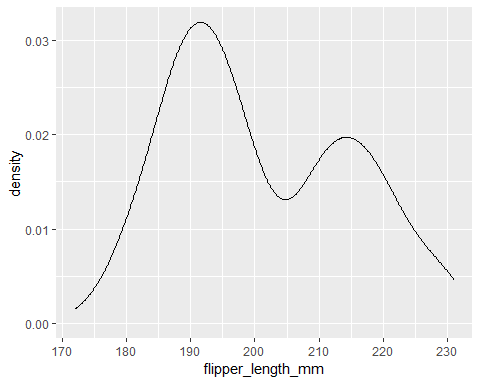
\includegraphics[width=0.5\linewidth]{livro_files/figure-latex/unnamed-chunk-195-1} 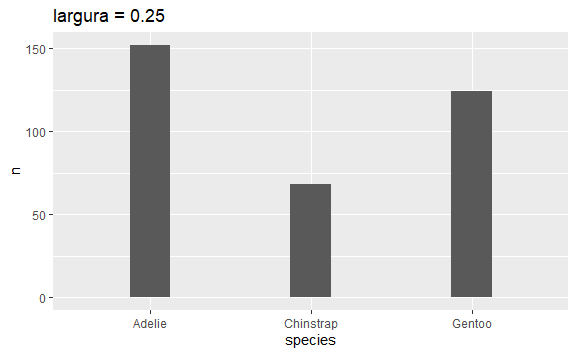
\includegraphics[width=0.5\linewidth]{livro_files/figure-latex/unnamed-chunk-195-2} \end{center}

Outra possibilidade para representação do gráfico de barras é inverter a direção das barras com a função \texttt{coord\_flip()}.

\begin{Shaded}
\begin{Highlighting}[]

\CommentTok{\# Barras vertical}
\FunctionTok{ggplot}\NormalTok{(}\AttributeTok{data =}\NormalTok{ penguins\_count, }
       \FunctionTok{aes}\NormalTok{(}\AttributeTok{x =}\NormalTok{ species, }\AttributeTok{y =}\NormalTok{ n)) }\SpecialCharTok{+}
  \FunctionTok{geom\_bar}\NormalTok{(}\AttributeTok{stat =} \StringTok{"identity"}\NormalTok{,}
           \AttributeTok{width =} \FloatTok{0.6}\NormalTok{)}

\CommentTok{\# Barras horizontal}
\FunctionTok{ggplot}\NormalTok{(}\AttributeTok{data =}\NormalTok{ penguins\_count, }
       \FunctionTok{aes}\NormalTok{(}\AttributeTok{x =}\NormalTok{ species, }\AttributeTok{y =}\NormalTok{ n)) }\SpecialCharTok{+}
  \FunctionTok{geom\_bar}\NormalTok{(}\AttributeTok{stat =} \StringTok{"identity"}\NormalTok{,}
           \AttributeTok{width =} \FloatTok{0.6}\NormalTok{) }\SpecialCharTok{+} 
  \FunctionTok{coord\_flip}\NormalTok{()}
\end{Highlighting}
\end{Shaded}

\begin{center}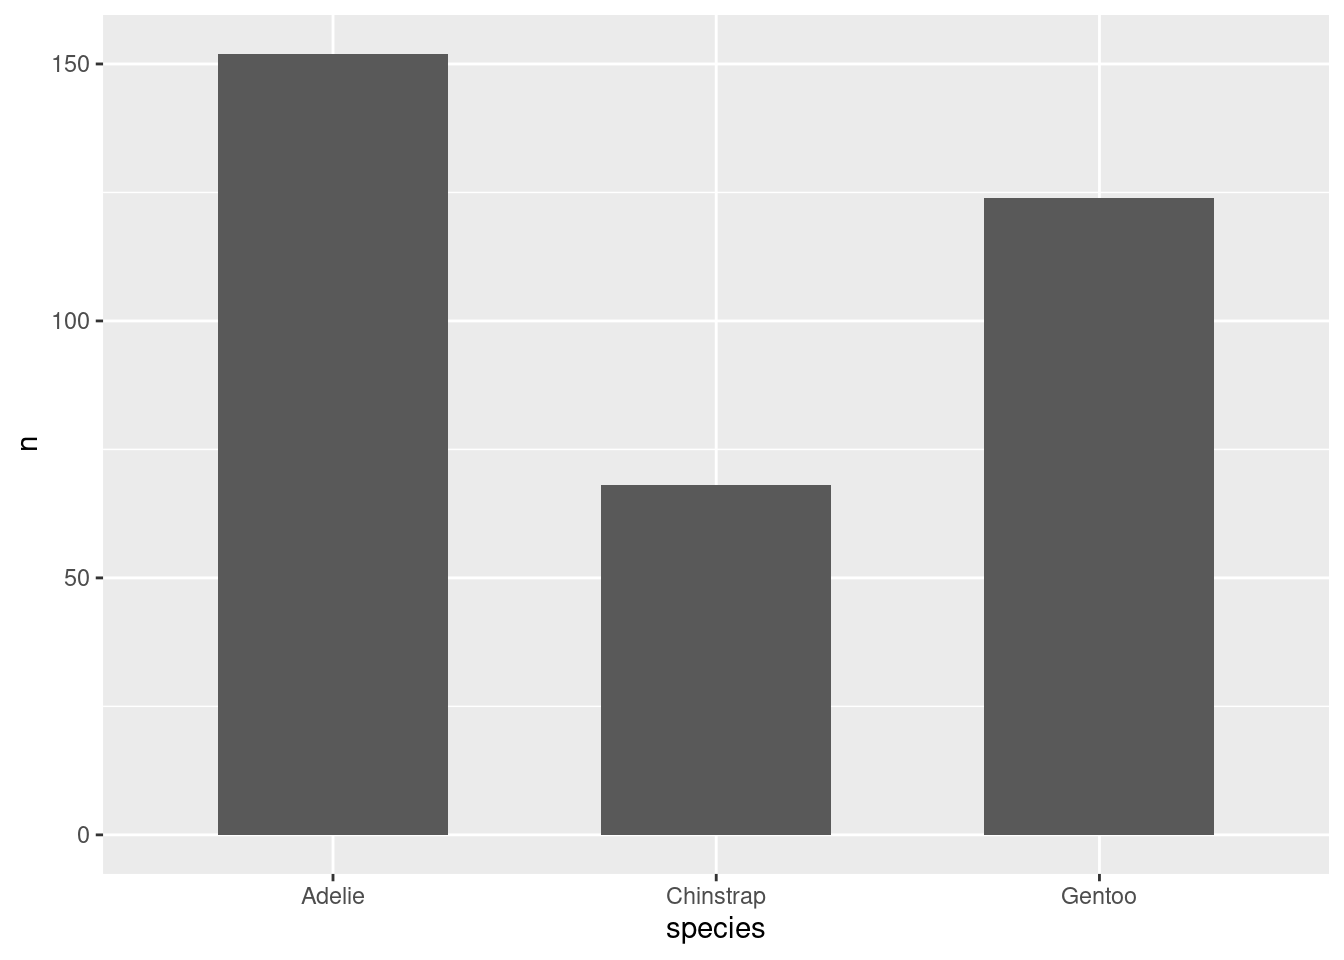
\includegraphics[width=0.5\linewidth]{livro_files/figure-latex/unnamed-chunk-196-1} 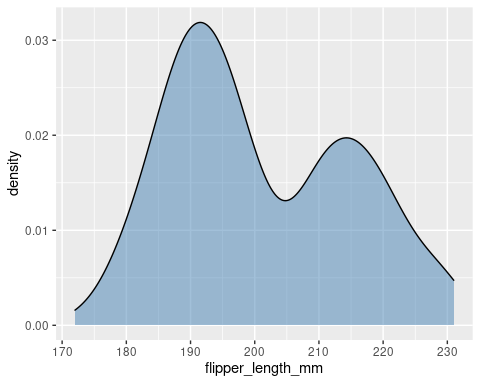
\includegraphics[width=0.5\linewidth]{livro_files/figure-latex/unnamed-chunk-196-2} \end{center}

É possível utilizar variáveis categóricas para definir cores e preenchimento e ilustrar, por exemplo, tratamentos ou espécies diferentes com os argumentos \texttt{fill} e \texttt{color}.

\begin{Shaded}
\begin{Highlighting}[]

\CommentTok{\# grafico de barras com preenchimento colorido}
\FunctionTok{ggplot}\NormalTok{(}\AttributeTok{data =}\NormalTok{ penguins\_count, }
       \FunctionTok{aes}\NormalTok{(}\AttributeTok{x =}\NormalTok{ species, }\AttributeTok{y =}\NormalTok{ n, }\AttributeTok{fill =}\NormalTok{ species)) }\SpecialCharTok{+}
  \FunctionTok{geom\_bar}\NormalTok{(}\AttributeTok{stat =} \StringTok{"identity"}\NormalTok{)}
\end{Highlighting}
\end{Shaded}

\begin{center}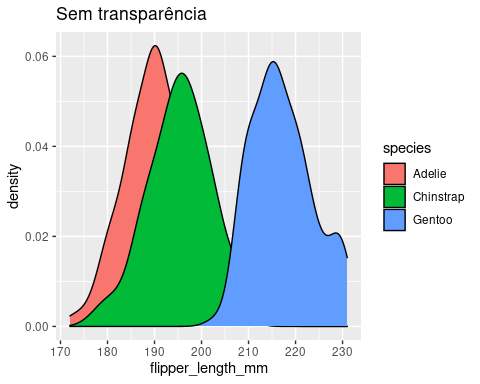
\includegraphics[width=0.7\linewidth]{livro_files/figure-latex/unnamed-chunk-197-1} \end{center}

\hypertarget{adicionando-medidas-de-variauxe7uxe3o}{%
\subsubsection{4.4.2. Adicionando medidas de variação}\label{adicionando-medidas-de-variauxe7uxe3o}}

Em algumas comparações, utilizar somente os valores absolutos pode não ser a visualização mais apropriadas como, por exemplo, em desenho de ANOVA (\textbf{Capítulo 7}). Desse modo, ao invés do valor máximo da barra representar o valor absoluto (e.g., número de indivíduos de uma espécies), ele vai representar o valor médio. Além disso, linhas adicionais (chamadas barras de erro) vão representar alguma medida de variação como desvio padrão, erro padrão, intervalo de confiança, entre outros. A função \texttt{Rmisc::summarySE()} permite realizar esses cálculos de maneira simples, como demonstrado no exemplo abaixo.

\begin{Shaded}
\begin{Highlighting}[]

\CommentTok{\# Calculando média e desvio padrão por grupo}

\NormalTok{penguins2 }\OtherTok{\textless{}{-}}\NormalTok{ penguins }\SpecialCharTok{\%\textgreater{}\%} 
  \FunctionTok{drop\_na}\NormalTok{(flipper\_length\_mm) }\CommentTok{\# remover valores ausentes na variável (NAs)}

\NormalTok{penguins\_mean }\OtherTok{\textless{}{-}} \FunctionTok{summarySE}\NormalTok{(penguins2, }
                           \AttributeTok{measurevar =} \StringTok{"flipper\_length\_mm"}\NormalTok{,}
                           \AttributeTok{groupvars =} \StringTok{"species"}\NormalTok{)}
\FunctionTok{head}\NormalTok{(penguins\_mean)}
\CommentTok{\#\textgreater{}     species   N flipper\_length\_mm       sd        se       ci}
\CommentTok{\#\textgreater{} 1    Adelie 151          189.9536 6.539457 0.5321735 1.051524}
\CommentTok{\#\textgreater{} 2 Chinstrap  68          195.8235 7.131894 0.8648692 1.726286}
\CommentTok{\#\textgreater{} 3    Gentoo 123          217.1870 6.484976 0.5847306 1.157533}

\CommentTok{\# Gráfico de barras com desvio padrão}
\FunctionTok{ggplot}\NormalTok{(}\AttributeTok{data =}\NormalTok{ penguins\_mean, }
       \FunctionTok{aes}\NormalTok{(}\AttributeTok{x =}\NormalTok{ species, }
           \AttributeTok{y =}\NormalTok{ flipper\_length\_mm, }
           \AttributeTok{fill =}\NormalTok{ species)) }\SpecialCharTok{+}
  \FunctionTok{geom\_bar}\NormalTok{(}\AttributeTok{stat =} \StringTok{"identity"}\NormalTok{, }\AttributeTok{alpha =} \FloatTok{0.4}\NormalTok{) }\SpecialCharTok{+}
  \FunctionTok{geom\_errorbar}\NormalTok{(}\FunctionTok{aes}\NormalTok{(}\AttributeTok{ymin =}\NormalTok{ flipper\_length\_mm }\SpecialCharTok{{-}}\NormalTok{ sd,}
                    \AttributeTok{ymax =}\NormalTok{ flipper\_length\_mm }\SpecialCharTok{+}\NormalTok{ sd),}
                \AttributeTok{width =} \FloatTok{0.1}\NormalTok{) }\SpecialCharTok{+} 
  \FunctionTok{geom\_point}\NormalTok{() }\SpecialCharTok{+}
  \FunctionTok{labs}\NormalTok{(}\AttributeTok{title =} \StringTok{"Barra de erro com desvio padrão"}\NormalTok{)}

\CommentTok{\# Gráfico de barras com intervalo de confiânça}
\FunctionTok{ggplot}\NormalTok{(}\AttributeTok{data =}\NormalTok{ penguins\_mean, }
       \FunctionTok{aes}\NormalTok{(}\AttributeTok{x =}\NormalTok{ species, }
           \AttributeTok{y =}\NormalTok{ flipper\_length\_mm, }
           \AttributeTok{fill =}\NormalTok{ species)) }\SpecialCharTok{+}
  \FunctionTok{geom\_bar}\NormalTok{(}\AttributeTok{stat =} \StringTok{"identity"}\NormalTok{, }\AttributeTok{alpha =} \FloatTok{0.4}\NormalTok{) }\SpecialCharTok{+}
  \FunctionTok{geom\_errorbar}\NormalTok{(}\FunctionTok{aes}\NormalTok{(}\AttributeTok{ymin =}\NormalTok{ flipper\_length\_mm }\SpecialCharTok{{-}}\NormalTok{ se,}
                    \AttributeTok{ymax =}\NormalTok{ flipper\_length\_mm }\SpecialCharTok{+}\NormalTok{ se),}
                \AttributeTok{width =} \FloatTok{0.1}\NormalTok{) }\SpecialCharTok{+} 
  \FunctionTok{geom\_point}\NormalTok{() }\SpecialCharTok{+}
  \FunctionTok{labs}\NormalTok{(}\AttributeTok{title =} \StringTok{"Barra de erro com erro padrão"}\NormalTok{)}
\end{Highlighting}
\end{Shaded}

\begin{center}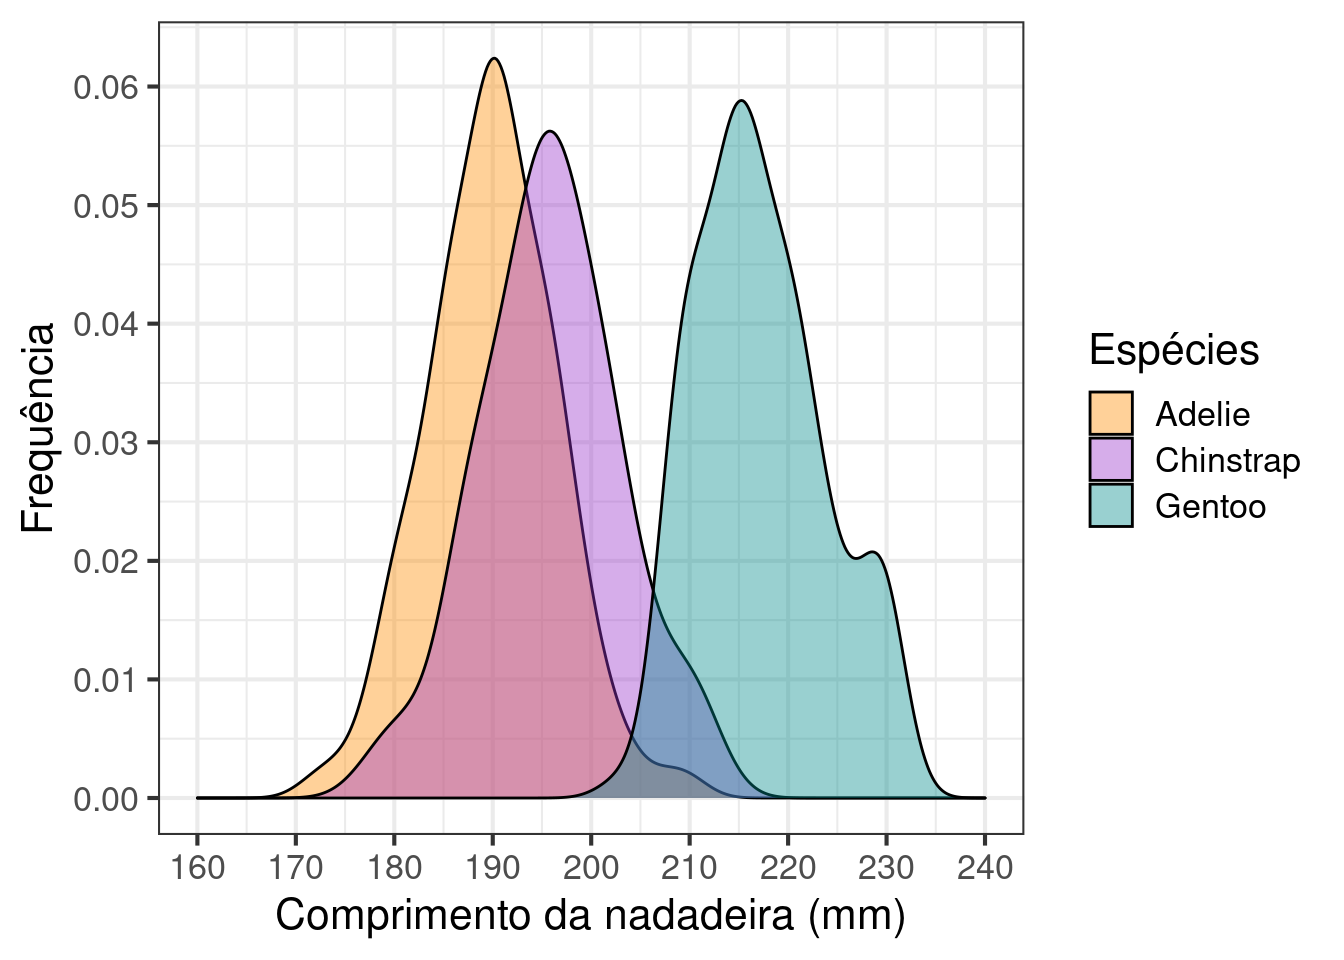
\includegraphics[width=0.7\linewidth]{livro_files/figure-latex/unnamed-chunk-198-1} 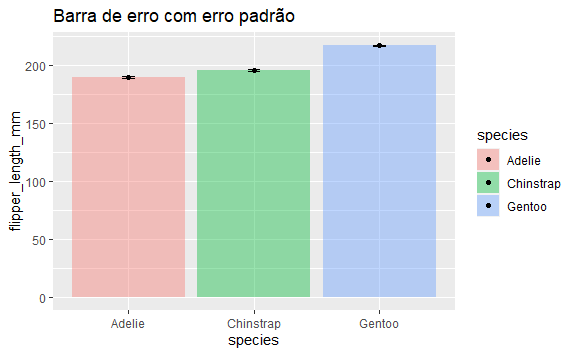
\includegraphics[width=0.7\linewidth]{livro_files/figure-latex/unnamed-chunk-198-2} \end{center}

\hypertarget{ajustes-finos-versuxe3o-personalizada-3}{%
\subsubsection{4.4.3. Ajustes finos (versão personalizada)}\label{ajustes-finos-versuxe3o-personalizada-3}}

\begin{Shaded}
\begin{Highlighting}[]

\FunctionTok{ggplot}\NormalTok{(}\AttributeTok{data =}\NormalTok{ penguins\_count, }
       \FunctionTok{aes}\NormalTok{(}\AttributeTok{x =}\NormalTok{ species, }\AttributeTok{y =}\NormalTok{ n, }\AttributeTok{fill =}\NormalTok{ species)) }\SpecialCharTok{+}
  \FunctionTok{geom\_bar}\NormalTok{(}\AttributeTok{stat =} \StringTok{"identity"}\NormalTok{) }\SpecialCharTok{+}
  \FunctionTok{geom\_label}\NormalTok{(}\FunctionTok{aes}\NormalTok{(}\AttributeTok{label =}\NormalTok{ n), }
             \AttributeTok{fill =} \StringTok{"white"}\NormalTok{) }\SpecialCharTok{+}
  \FunctionTok{theme\_bw}\NormalTok{(}\AttributeTok{base\_size =} \DecValTok{16}\NormalTok{) }\SpecialCharTok{+}
  \FunctionTok{scale\_fill\_manual}\NormalTok{(}\AttributeTok{values =} \FunctionTok{c}\NormalTok{(}\StringTok{"darkorange"}\NormalTok{, }\StringTok{"purple"}\NormalTok{, }\StringTok{"cyan4"}\NormalTok{)) }\SpecialCharTok{+}
  \FunctionTok{labs}\NormalTok{(}\AttributeTok{x =} \StringTok{"Espécie"}\NormalTok{, }\AttributeTok{y =} \StringTok{"Número de indivíduos"}\NormalTok{, }\AttributeTok{fill =} \StringTok{"Espécie"}\NormalTok{)}
\end{Highlighting}
\end{Shaded}

\begin{center}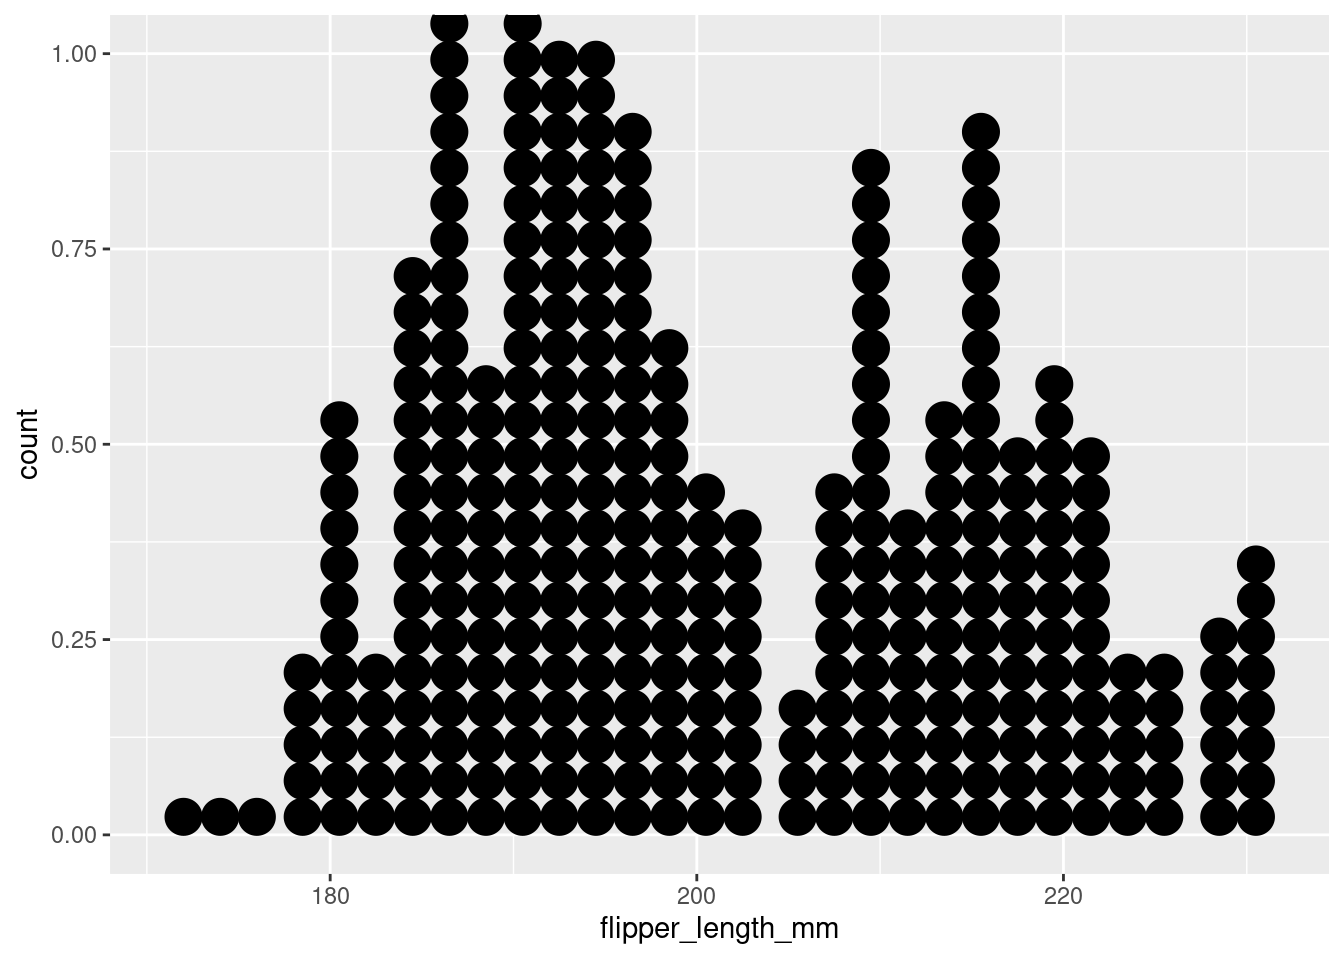
\includegraphics[width=0.7\linewidth]{livro_files/figure-latex/unnamed-chunk-199-1} \end{center}

\hypertarget{gruxe1fico-de-setores-pie-chart-e-donut-chart}{%
\subsection{\texorpdfstring{4.5. Gráfico de setores (\emph{pie chart} e \emph{donut chart})}{4.5. Gráfico de setores (pie chart e donut chart)}}\label{gruxe1fico-de-setores-pie-chart-e-donut-chart}}

Além do gráfico de barras, o \href{https://pt.wikipedia.org/wiki/Gr\%C3\%A1fico_de_setores}{gráfico de setores} representa uma alternativa para comparar a proporção entre categorias. Tais gráficos podem ser representados como \emph{pie charts} ou \emph{donut charts}, como demonstrado abaixo. No exemplo abaixo, utilizamos a mesma comparação realizada no item 4.3.3 acima. Porém, os valores de contagem (número de indivíduos por espécie) devem ser transformados previamente em proporção.

\hypertarget{gruxe1fico-de-setores-pie-chart}{%
\subsubsection{\texorpdfstring{4.5.1. Gráfico de setores (\emph{pie chart})}{4.5.1. Gráfico de setores (pie chart)}}\label{gruxe1fico-de-setores-pie-chart}}

\begin{Shaded}
\begin{Highlighting}[]
\CommentTok{\# Cálculo da proporção}

\NormalTok{penguins\_prop }\OtherTok{\textless{}{-}}\NormalTok{ penguins }\SpecialCharTok{\%\textgreater{}\%}
\NormalTok{  dplyr}\SpecialCharTok{::}\FunctionTok{count}\NormalTok{(species) }\SpecialCharTok{\%\textgreater{}\%} 
\NormalTok{  dplyr}\SpecialCharTok{::}\FunctionTok{mutate}\NormalTok{(}\AttributeTok{prop =} \FunctionTok{round}\NormalTok{(n}\SpecialCharTok{/}\FunctionTok{sum}\NormalTok{(n), }\DecValTok{4}\NormalTok{)}\SpecialCharTok{*}\DecValTok{100}\NormalTok{)}

\CommentTok{\# Pie chart}
\FunctionTok{ggplot}\NormalTok{(}\AttributeTok{data =}\NormalTok{ penguins\_prop, }\FunctionTok{aes}\NormalTok{(}\AttributeTok{x =} \StringTok{""}\NormalTok{, }\AttributeTok{y =}\NormalTok{ prop, }\AttributeTok{fill =}\NormalTok{ species)) }\SpecialCharTok{+} 
  \FunctionTok{geom\_bar}\NormalTok{(}\AttributeTok{stat =} \StringTok{"identity"}\NormalTok{, }\AttributeTok{color =} \StringTok{"white"}\NormalTok{) }\SpecialCharTok{+}
  \FunctionTok{coord\_polar}\NormalTok{(}\StringTok{"y"}\NormalTok{, }\AttributeTok{start =} \DecValTok{0}\NormalTok{) }\SpecialCharTok{+}
  \FunctionTok{geom\_text}\NormalTok{(}\FunctionTok{aes}\NormalTok{(}\AttributeTok{label =} \FunctionTok{paste0}\NormalTok{(prop, }\StringTok{"\%"}\NormalTok{)), }\AttributeTok{color =} \StringTok{"white"}\NormalTok{, }
            \AttributeTok{position =} \FunctionTok{position\_stack}\NormalTok{(}\AttributeTok{vjust =} \FloatTok{0.5}\NormalTok{), }\AttributeTok{size =} \DecValTok{8}\NormalTok{) }\SpecialCharTok{+}
  \FunctionTok{scale\_fill\_manual}\NormalTok{(}\AttributeTok{values =} \FunctionTok{c}\NormalTok{(}\StringTok{"darkorange"}\NormalTok{, }\StringTok{"purple"}\NormalTok{, }\StringTok{"cyan4"}\NormalTok{)) }\SpecialCharTok{+}
  \FunctionTok{theme\_void}\NormalTok{() }\SpecialCharTok{+}
  \FunctionTok{labs}\NormalTok{(}\AttributeTok{fill =} \StringTok{"Espécie"}\NormalTok{)}
\end{Highlighting}
\end{Shaded}

\begin{center}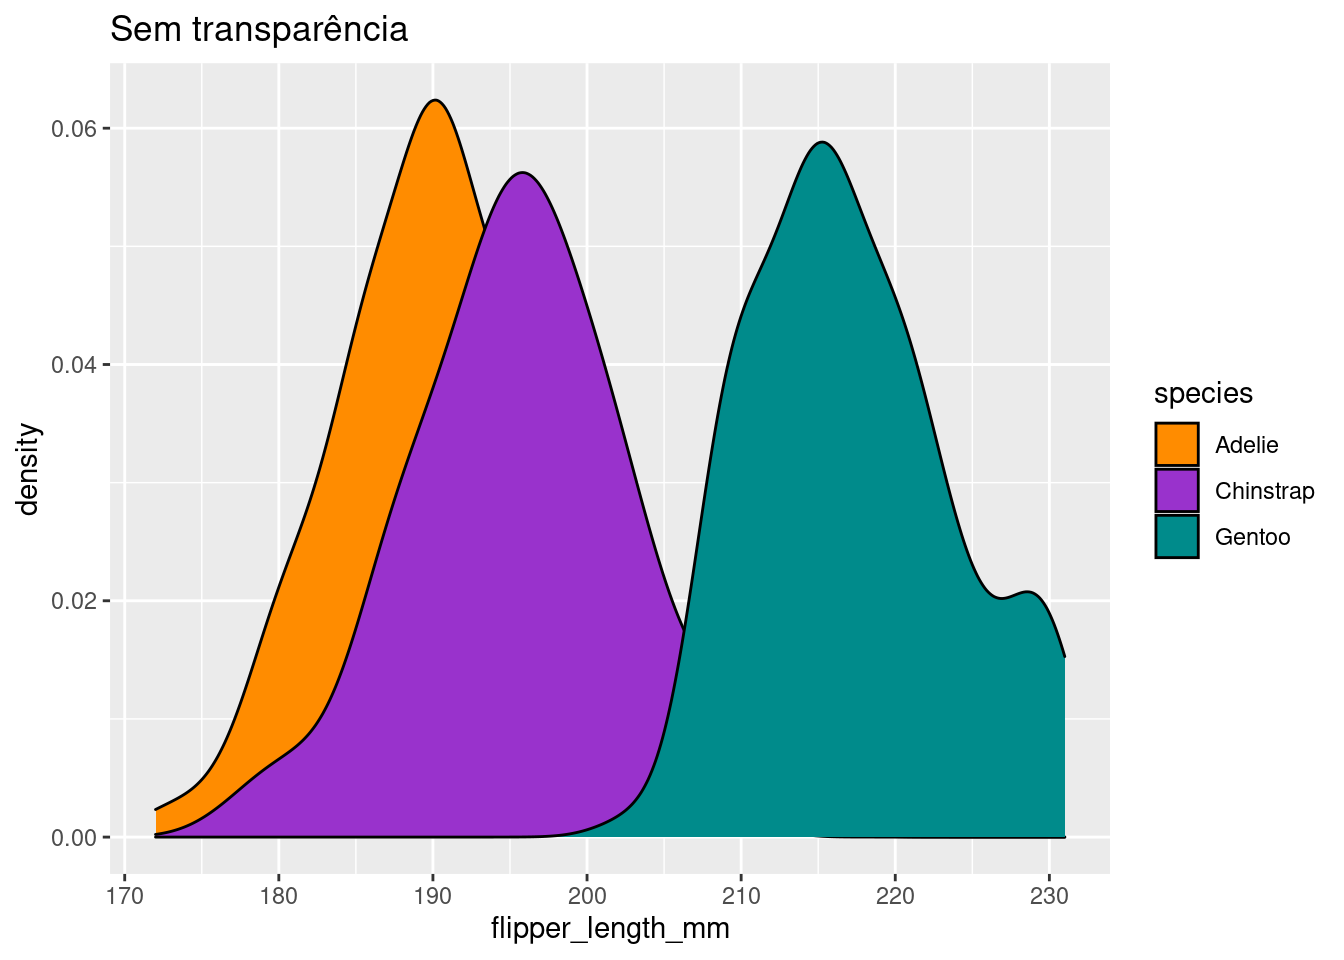
\includegraphics[width=0.7\linewidth]{livro_files/figure-latex/unnamed-chunk-200-1} \end{center}

\hypertarget{gruxe1fico-de-setores-donut-chart}{%
\subsubsection{\texorpdfstring{4.5.2. Gráfico de setores (\emph{donut chart})}{4.5.2. Gráfico de setores (donut chart)}}\label{gruxe1fico-de-setores-donut-chart}}

\begin{Shaded}
\begin{Highlighting}[]

\FunctionTok{ggplot}\NormalTok{(}\AttributeTok{data =}\NormalTok{ penguins\_prop, }\FunctionTok{aes}\NormalTok{(}\AttributeTok{x =} \DecValTok{2}\NormalTok{, }\AttributeTok{y =}\NormalTok{ prop, }\AttributeTok{fill =}\NormalTok{ species)) }\SpecialCharTok{+}
  \FunctionTok{geom\_bar}\NormalTok{(}\AttributeTok{stat =} \StringTok{"identity"}\NormalTok{) }\SpecialCharTok{+}
  \FunctionTok{coord\_polar}\NormalTok{(}\AttributeTok{theta =} \StringTok{"y"}\NormalTok{, }\AttributeTok{start =} \DecValTok{0}\NormalTok{) }\SpecialCharTok{+}
  \FunctionTok{geom\_text}\NormalTok{(}\FunctionTok{aes}\NormalTok{(}\AttributeTok{label =} \FunctionTok{paste0}\NormalTok{(prop, }\StringTok{"\%"}\NormalTok{)), }\AttributeTok{color =} \StringTok{"white"}\NormalTok{,}
            \AttributeTok{position =} \FunctionTok{position\_stack}\NormalTok{(}\AttributeTok{vjust =}\NormalTok{ .}\DecValTok{5}\NormalTok{), }\AttributeTok{size =} \DecValTok{5}\NormalTok{) }\SpecialCharTok{+}
  \FunctionTok{scale\_fill\_manual}\NormalTok{(}\AttributeTok{values =} \FunctionTok{c}\NormalTok{(}\StringTok{"darkorange"}\NormalTok{, }\StringTok{"purple"}\NormalTok{, }\StringTok{"cyan4"}\NormalTok{)) }\SpecialCharTok{+}
  \FunctionTok{xlim}\NormalTok{(}\DecValTok{0}\NormalTok{, }\FloatTok{2.5}\NormalTok{) }\SpecialCharTok{+}
  \FunctionTok{theme\_void}\NormalTok{() }\SpecialCharTok{+}
  \FunctionTok{theme}\NormalTok{(}\AttributeTok{legend.position =} \FunctionTok{c}\NormalTok{(.}\DecValTok{5}\NormalTok{, .}\DecValTok{5}\NormalTok{),}
        \AttributeTok{legend.title =} \FunctionTok{element\_text}\NormalTok{(}\AttributeTok{size =} \DecValTok{20}\NormalTok{),}
        \AttributeTok{legend.text =} \FunctionTok{element\_text}\NormalTok{(}\AttributeTok{size =} \DecValTok{15}\NormalTok{)) }\SpecialCharTok{+}
  \FunctionTok{labs}\NormalTok{(}\AttributeTok{fill =} \StringTok{"Espécie"}\NormalTok{)}
\end{Highlighting}
\end{Shaded}

\begin{center}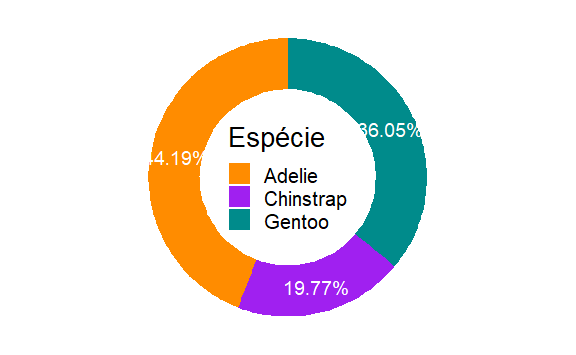
\includegraphics[width=0.7\linewidth]{livro_files/figure-latex/unnamed-chunk-201-1} \end{center}

\hypertarget{comparando-gruxe1ficos-de-setores-com-gruxe1fico-de-barras}{%
\subsubsection{4.5.3. Comparando gráficos de setores com gráfico de barras}\label{comparando-gruxe1ficos-de-setores-com-gruxe1fico-de-barras}}

O mesmo conjunto de dados pode ser visualizado de diferentes formas. Não diferente, a comparação da proporção de ocorrências de diferentes categorias pode ser feita de várias maneiras. Abaixo, fizemos a comparação da proporção de indivíduos por cada uma das três espécies dos dados \texttt{penguins}.

\begin{Shaded}
\begin{Highlighting}[]


\FunctionTok{ggplot}\NormalTok{(}\AttributeTok{data =}\NormalTok{ penguins\_prop, }\FunctionTok{aes}\NormalTok{(}\AttributeTok{x =} \StringTok{""}\NormalTok{, }\AttributeTok{y =}\NormalTok{ prop, }\AttributeTok{fill =}\NormalTok{ species)) }\SpecialCharTok{+} 
  \FunctionTok{geom\_bar}\NormalTok{(}\AttributeTok{stat =} \StringTok{"identity"}\NormalTok{, }\AttributeTok{color =} \StringTok{"white"}\NormalTok{) }\SpecialCharTok{+}
  \FunctionTok{coord\_polar}\NormalTok{(}\StringTok{"y"}\NormalTok{, }\AttributeTok{start =} \DecValTok{0}\NormalTok{) }\SpecialCharTok{+}
  \FunctionTok{geom\_text}\NormalTok{(}\FunctionTok{aes}\NormalTok{(}\AttributeTok{label =} \FunctionTok{paste0}\NormalTok{(prop, }\StringTok{"\%"}\NormalTok{)), }\AttributeTok{color =} \StringTok{"white"}\NormalTok{, }
            \AttributeTok{position =} \FunctionTok{position\_stack}\NormalTok{(}\AttributeTok{vjust =} \FloatTok{0.5}\NormalTok{), }\AttributeTok{size =} \DecValTok{3}\NormalTok{) }\SpecialCharTok{+}
  \FunctionTok{scale\_fill\_manual}\NormalTok{(}\AttributeTok{values =} \FunctionTok{c}\NormalTok{(}\StringTok{"darkorange"}\NormalTok{, }\StringTok{"purple"}\NormalTok{, }\StringTok{"cyan4"}\NormalTok{)) }\SpecialCharTok{+}
  \FunctionTok{theme\_void}\NormalTok{() }\SpecialCharTok{+}
  \FunctionTok{labs}\NormalTok{(}\AttributeTok{title =} \StringTok{"Pie chart"}\NormalTok{, }\AttributeTok{fill =} \StringTok{"Espécies"}\NormalTok{) }\OtherTok{{-}\textgreater{}}\NormalTok{ g\_pie}

\FunctionTok{ggplot}\NormalTok{(}\AttributeTok{data =}\NormalTok{ penguins\_prop, }\FunctionTok{aes}\NormalTok{(}\AttributeTok{x =} \DecValTok{2}\NormalTok{, }\AttributeTok{y =}\NormalTok{ prop, }\AttributeTok{fill =}\NormalTok{ species)) }\SpecialCharTok{+}
  \FunctionTok{geom\_bar}\NormalTok{(}\AttributeTok{stat =} \StringTok{"identity"}\NormalTok{) }\SpecialCharTok{+}
  \FunctionTok{coord\_polar}\NormalTok{(}\AttributeTok{theta =} \StringTok{"y"}\NormalTok{, }\AttributeTok{start =} \DecValTok{0}\NormalTok{) }\SpecialCharTok{+}
  \FunctionTok{geom\_text}\NormalTok{(}\FunctionTok{aes}\NormalTok{(}\AttributeTok{label =} \FunctionTok{paste0}\NormalTok{(prop, }\StringTok{"\%"}\NormalTok{)), }\AttributeTok{color =} \StringTok{"white"}\NormalTok{,}
            \AttributeTok{position =} \FunctionTok{position\_stack}\NormalTok{(}\AttributeTok{vjust =}\NormalTok{ .}\DecValTok{5}\NormalTok{), }\AttributeTok{size =}\DecValTok{3}\NormalTok{) }\SpecialCharTok{+}
  \FunctionTok{scale\_fill\_manual}\NormalTok{(}\AttributeTok{values =} \FunctionTok{c}\NormalTok{(}\StringTok{"darkorange"}\NormalTok{, }\StringTok{"purple"}\NormalTok{, }\StringTok{"cyan4"}\NormalTok{)) }\SpecialCharTok{+}
  \FunctionTok{xlim}\NormalTok{(}\DecValTok{0}\NormalTok{, }\FloatTok{2.5}\NormalTok{) }\SpecialCharTok{+}
  \FunctionTok{theme\_void}\NormalTok{() }\SpecialCharTok{+}
  \FunctionTok{theme}\NormalTok{(}\AttributeTok{legend.position =} \StringTok{"none"}\NormalTok{) }\SpecialCharTok{+}
  \FunctionTok{labs}\NormalTok{(}\AttributeTok{title =} \StringTok{"Donut chart"}\NormalTok{, }\AttributeTok{fill =} \StringTok{"Espécies"}\NormalTok{) }\OtherTok{{-}\textgreater{}}\NormalTok{ g\_donut}


\FunctionTok{ggplot}\NormalTok{(}\AttributeTok{data =}\NormalTok{ penguins\_prop, }
       \FunctionTok{aes}\NormalTok{(}\AttributeTok{x =}\NormalTok{ species, }\AttributeTok{y =}\NormalTok{ prop, }\AttributeTok{fill =}\NormalTok{ species)) }\SpecialCharTok{+}
  \FunctionTok{geom\_bar}\NormalTok{(}\AttributeTok{stat =} \StringTok{"identity"}\NormalTok{) }\SpecialCharTok{+}
  \FunctionTok{geom\_label}\NormalTok{(}\FunctionTok{aes}\NormalTok{(}\AttributeTok{label =}\NormalTok{ prop), }
             \AttributeTok{fill =} \StringTok{"white"}\NormalTok{) }\SpecialCharTok{+}
  \FunctionTok{theme\_bw}\NormalTok{() }\SpecialCharTok{+}
  \FunctionTok{scale\_fill\_manual}\NormalTok{(}\AttributeTok{values =} \FunctionTok{c}\NormalTok{(}\StringTok{"darkorange"}\NormalTok{, }\StringTok{"purple"}\NormalTok{, }\StringTok{"cyan4"}\NormalTok{)) }\SpecialCharTok{+}
  \FunctionTok{labs}\NormalTok{(}\AttributeTok{title =} \StringTok{"Gráfico de Barras (Horizonal)"}\NormalTok{, }\AttributeTok{x =} \StringTok{"Espécies"}\NormalTok{, }\AttributeTok{y =} \StringTok{"Número de indivíduos"}\NormalTok{, }\AttributeTok{fill =} \StringTok{"Espécies"}\NormalTok{)}\SpecialCharTok{+}
  \FunctionTok{theme}\NormalTok{(}\AttributeTok{legend.position =} \StringTok{"none"}\NormalTok{)}\OtherTok{{-}\textgreater{}}\NormalTok{ g\_bar\_h}

\FunctionTok{ggplot}\NormalTok{(}\AttributeTok{data =}\NormalTok{ penguins\_prop, }
       \FunctionTok{aes}\NormalTok{(}\AttributeTok{x =}\NormalTok{ species, }\AttributeTok{y =}\NormalTok{ prop, }\AttributeTok{fill =}\NormalTok{ species)) }\SpecialCharTok{+}
  \FunctionTok{geom\_bar}\NormalTok{(}\AttributeTok{stat =} \StringTok{"identity"}\NormalTok{) }\SpecialCharTok{+}
  \FunctionTok{geom\_label}\NormalTok{(}\FunctionTok{aes}\NormalTok{(}\AttributeTok{label =}\NormalTok{ prop), }
             \AttributeTok{fill =} \StringTok{"white"}\NormalTok{) }\SpecialCharTok{+}
  \FunctionTok{theme\_bw}\NormalTok{() }\SpecialCharTok{+}
  \FunctionTok{coord\_flip}\NormalTok{()}\SpecialCharTok{+}
  \FunctionTok{scale\_fill\_manual}\NormalTok{(}\AttributeTok{values =} \FunctionTok{c}\NormalTok{(}\StringTok{"darkorange"}\NormalTok{, }\StringTok{"purple"}\NormalTok{, }\StringTok{"cyan4"}\NormalTok{)) }\SpecialCharTok{+}
  \FunctionTok{labs}\NormalTok{(}\AttributeTok{title =} \StringTok{"Gráfico de Barras (Vertical)"}\NormalTok{, }\AttributeTok{x =} \StringTok{"Espécies"}\NormalTok{, }\AttributeTok{y =} \StringTok{"Número de indivíduos"}\NormalTok{, }\AttributeTok{fill =} \StringTok{"Espécies"}\NormalTok{) }\SpecialCharTok{+}
  \FunctionTok{theme}\NormalTok{(}\AttributeTok{legend.position =} \StringTok{"none"}\NormalTok{)}\OtherTok{{-}\textgreater{}}\NormalTok{ g\_bar\_v}


\FunctionTok{grid.arrange}\NormalTok{(g\_pie, g\_donut, g\_bar\_h, g\_bar\_v, }\AttributeTok{nrow=}\DecValTok{2}\NormalTok{)}
\end{Highlighting}
\end{Shaded}

\begin{center}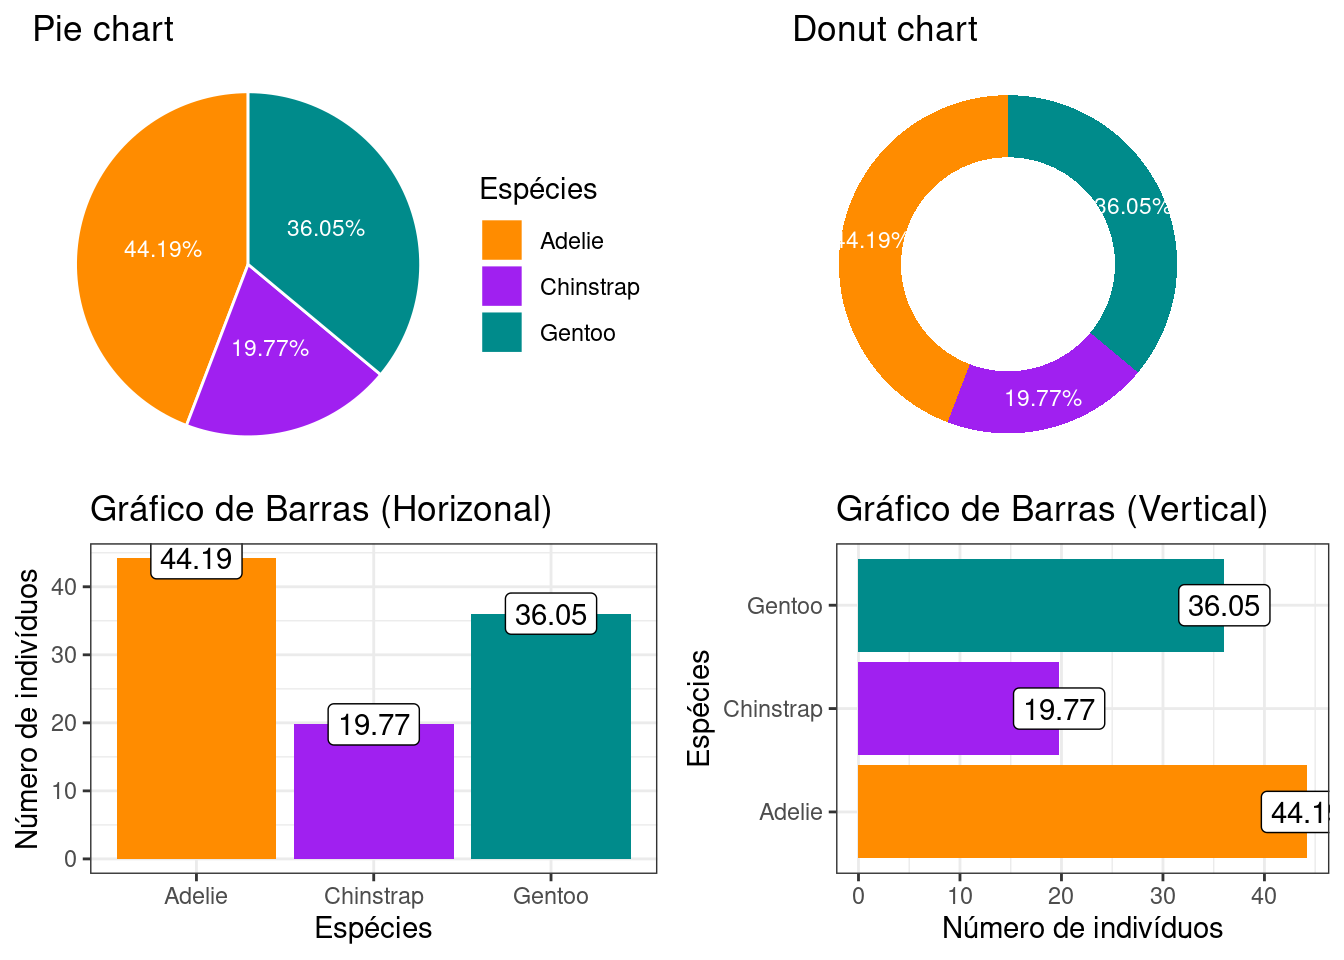
\includegraphics[width=1\linewidth]{livro_files/figure-latex/unnamed-chunk-202-1} \end{center}

\hypertarget{principais-camadas-utilizadas-no-gruxe1fico-de-barras-e-de-setores-geom_bar}{%
\subsubsection{\texorpdfstring{4.5.4. Principais camadas utilizadas no gráfico de barras e de setores: \texttt{geom\_bar()}}{4.5.4. Principais camadas utilizadas no gráfico de barras e de setores: geom\_bar()}}\label{principais-camadas-utilizadas-no-gruxe1fico-de-barras-e-de-setores-geom_bar}}

\begin{itemize}
\item
  \texttt{aes()}:

  \begin{itemize}
  \item
    Eixo X: variável categórica (\emph{species})
  \item
    Eixo Y: variável contínua (\emph{flipper\_length\_mm})
  \item
    Preenchimento (\emph{fill}): a variável categórica (\emph{species}) define a cor do preenchimento e os níveis dentro desta categoria determinam o número de cores que devem ser indicadas no \texttt{scale\_fill\_manual()}.
  \end{itemize}
\item
  \texttt{geom():}

  \begin{itemize}
  \item
    \texttt{geom\_bar()}

    \begin{itemize}
    \item
      Transparência das barras (\texttt{alpha}): 0,4 (varia de 0, trasparência máxima, a 1, sem trasparência)
    \item
      \texttt{stat}: é necessário usar o argumento ``identity'' quando os valores do eixo Y são adicionados pelo usuário
    \end{itemize}
  \item
    \texttt{geom\_label()}

    \begin{itemize}
    \tightlist
    \item
      forma geométrica que adiciona rótulo dos valores absolutos das barras por categoria (\emph{species})
    \end{itemize}
  \item
    \texttt{geom\_errorbar()}

    \begin{itemize}
    \tightlist
    \item
      \texttt{ymin}e \texttt{ymax}delimitam os valores mínimos e máximos, respectivamente, das barras de erro. Tais valores são representados pelo valor da média menos (no caso do ymin) ou mais (no caso do ymax) o valor do intervalo de confiança, desvio ou erro padrão.
    \end{itemize}
  \end{itemize}
\item
  \texttt{coord\_polar()}: sistema de coordenadas para gerar barras circulares sobrepostas (\emph{stacked}) que são usadas nos gráficos de setores (\emph{pie chart} e \emph{donut chart})

  \begin{itemize}
  \tightlist
  \item
    o argumento \texttt{start\ =\ 0} indica o local de início do gráfico que, neste caso, começa na ``hora'' 0 em um ``relógio'' de 12 horas.
  \end{itemize}
\item
  \texttt{scale()}:

  \begin{itemize}
  \tightlist
  \item
    \texttt{scale\_fill\_manual()} para definir manualmente as cores de preferência do usuário
  \end{itemize}
\item
  \texttt{theme()}: \texttt{theme\_bw()}para selecionar o tema com fundo branco e \texttt{labs()} para personalizar o títulos dos eixos X e Y, e da legenda.
\end{itemize}

\hypertarget{gruxe1fico-de-caixa-boxplot}{%
\subsection{\texorpdfstring{4.6. Gráfico de caixa (\emph{boxplot})}{4.6. Gráfico de caixa (boxplot)}}\label{gruxe1fico-de-caixa-boxplot}}

O \href{https://pt.wikipedia.org/wiki/Diagrama_de_caixa}{boxplot}, conhecido amplamente nos artigos e livros de ecologia, é uma visualização gráfica que sintetiza informações importantes de dados contínuos como mediana e variação (quartil 1-3, ver Figura 2).

\begin{figure}

{\centering 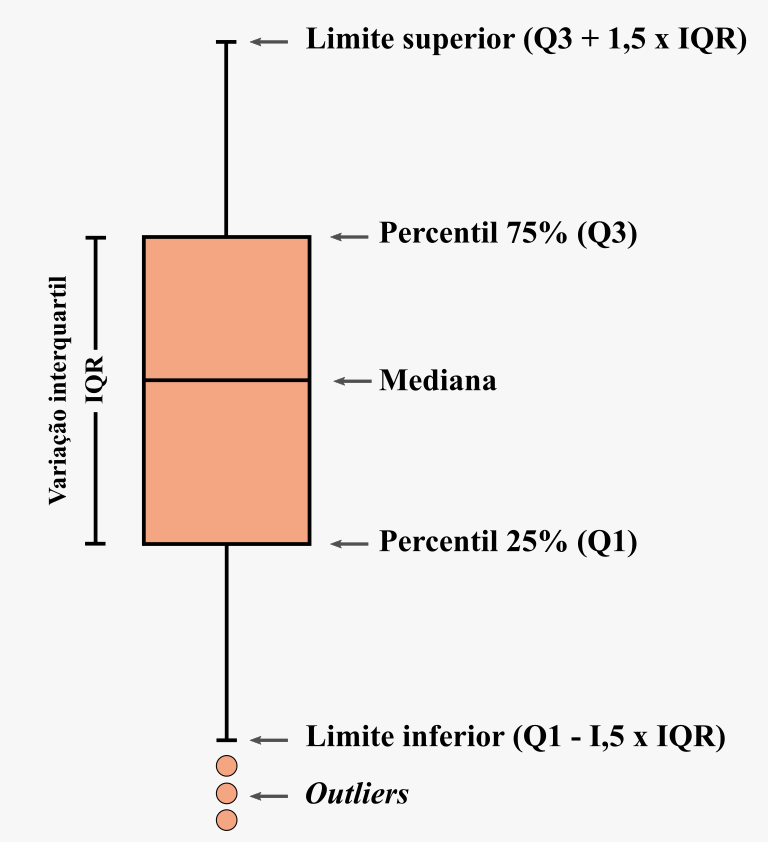
\includegraphics[width=0.7\linewidth]{img/fig_boxplot} 

}

\caption{Estrutura e elementos do boxplot}\label{fig:fig-boxplot}
\end{figure}

\hypertarget{versuxe3o-padruxe3o-4}{%
\subsubsection{4.6.1. Versão padrão}\label{versuxe3o-padruxe3o-4}}

Vamos plotar uma variável contínua (flipper\_length\_mm) no eixo y em função de uma variável categórica no eixo x (species). A definição de qual coluna do banco de dados é a x e qual é a y é feita dentro do comendo \texttt{aes()}.

\begin{Shaded}
\begin{Highlighting}[]

\FunctionTok{ggplot}\NormalTok{(penguins, }\FunctionTok{aes}\NormalTok{(}\AttributeTok{y =}\NormalTok{ flipper\_length\_mm, }\AttributeTok{x =}\NormalTok{ species)) }\SpecialCharTok{+}
  \FunctionTok{geom\_boxplot}\NormalTok{()}
\end{Highlighting}
\end{Shaded}

\begin{center}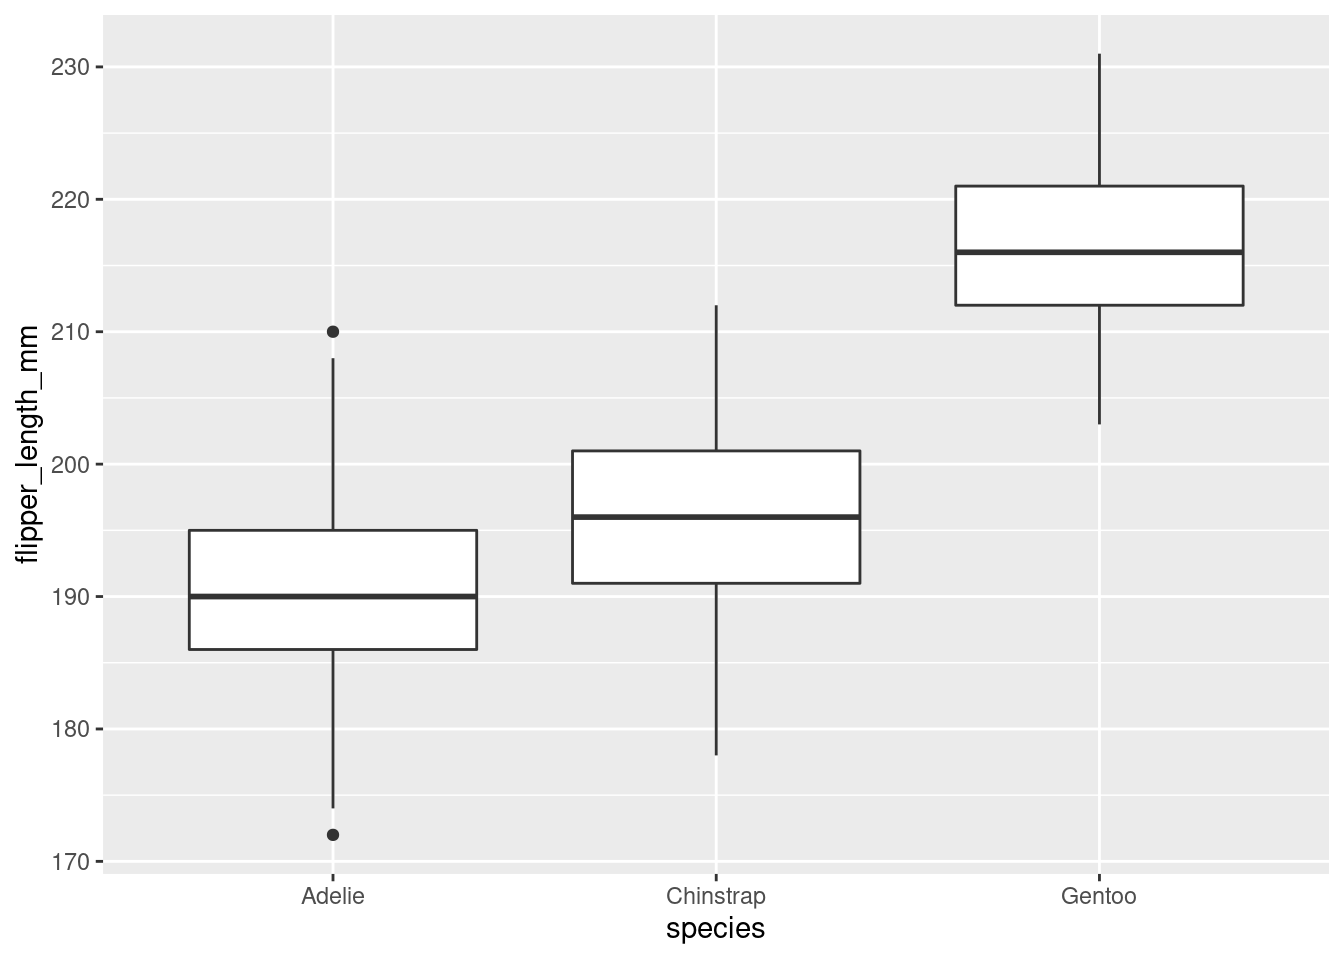
\includegraphics[width=0.7\linewidth]{livro_files/figure-latex/unnamed-chunk-203-1} \end{center}

É possível destacar os pontos referentes aos outliers (se houver) com o argumento \textbf{outlier.color}. Caso tenha interesse, é possível também remover os outliers do gráfico.

\begin{Shaded}
\begin{Highlighting}[]

\FunctionTok{ggplot}\NormalTok{(penguins, }\FunctionTok{aes}\NormalTok{(}\AttributeTok{y =}\NormalTok{ flipper\_length\_mm, }\AttributeTok{x =}\NormalTok{ species)) }\SpecialCharTok{+}
  \FunctionTok{geom\_boxplot}\NormalTok{(}\AttributeTok{outlier.color =} \StringTok{"red"}\NormalTok{)}\SpecialCharTok{+}
  \FunctionTok{labs}\NormalTok{(}\AttributeTok{title =} \StringTok{"outliers vermelhos"}\NormalTok{)}

\FunctionTok{ggplot}\NormalTok{(penguins, }\FunctionTok{aes}\NormalTok{(}\AttributeTok{y =}\NormalTok{ flipper\_length\_mm, }\AttributeTok{x =}\NormalTok{ species)) }\SpecialCharTok{+}
  \FunctionTok{geom\_boxplot}\NormalTok{(}\AttributeTok{outlier.shape =} \ConstantTok{NA}\NormalTok{)}\SpecialCharTok{+}
  \FunctionTok{labs}\NormalTok{(}\AttributeTok{title =} \StringTok{"outliers removidos"}\NormalTok{)}
\end{Highlighting}
\end{Shaded}

\begin{center}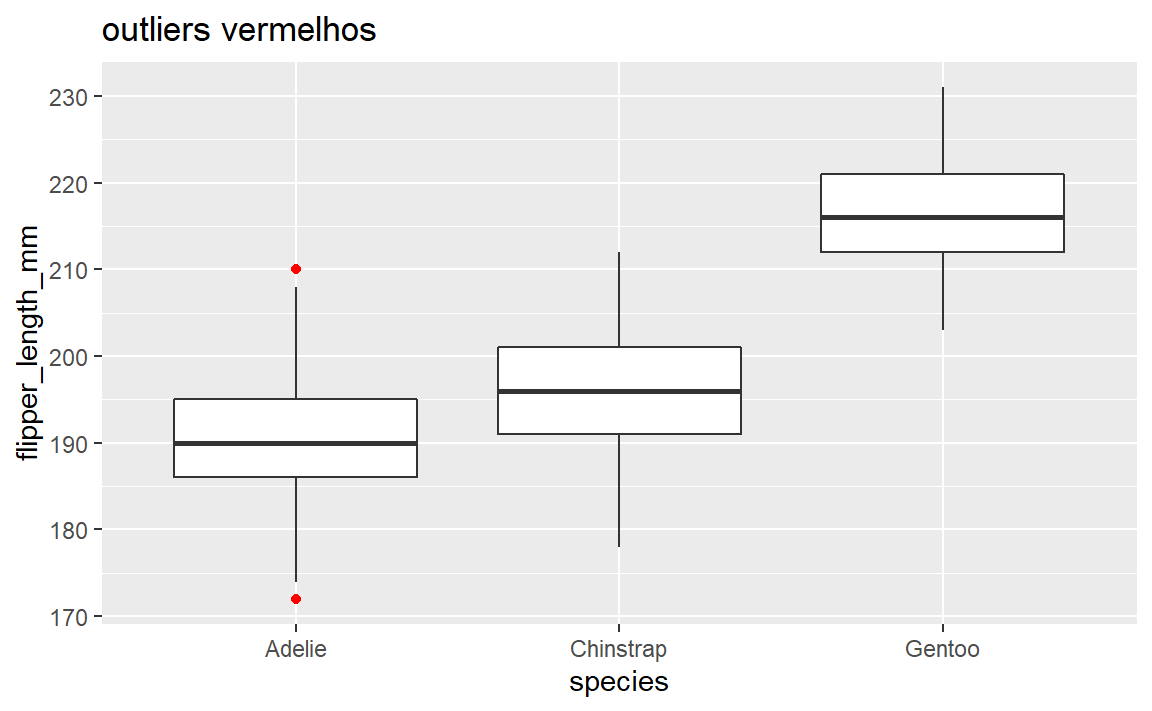
\includegraphics[width=0.7\linewidth]{livro_files/figure-latex/unnamed-chunk-204-1} 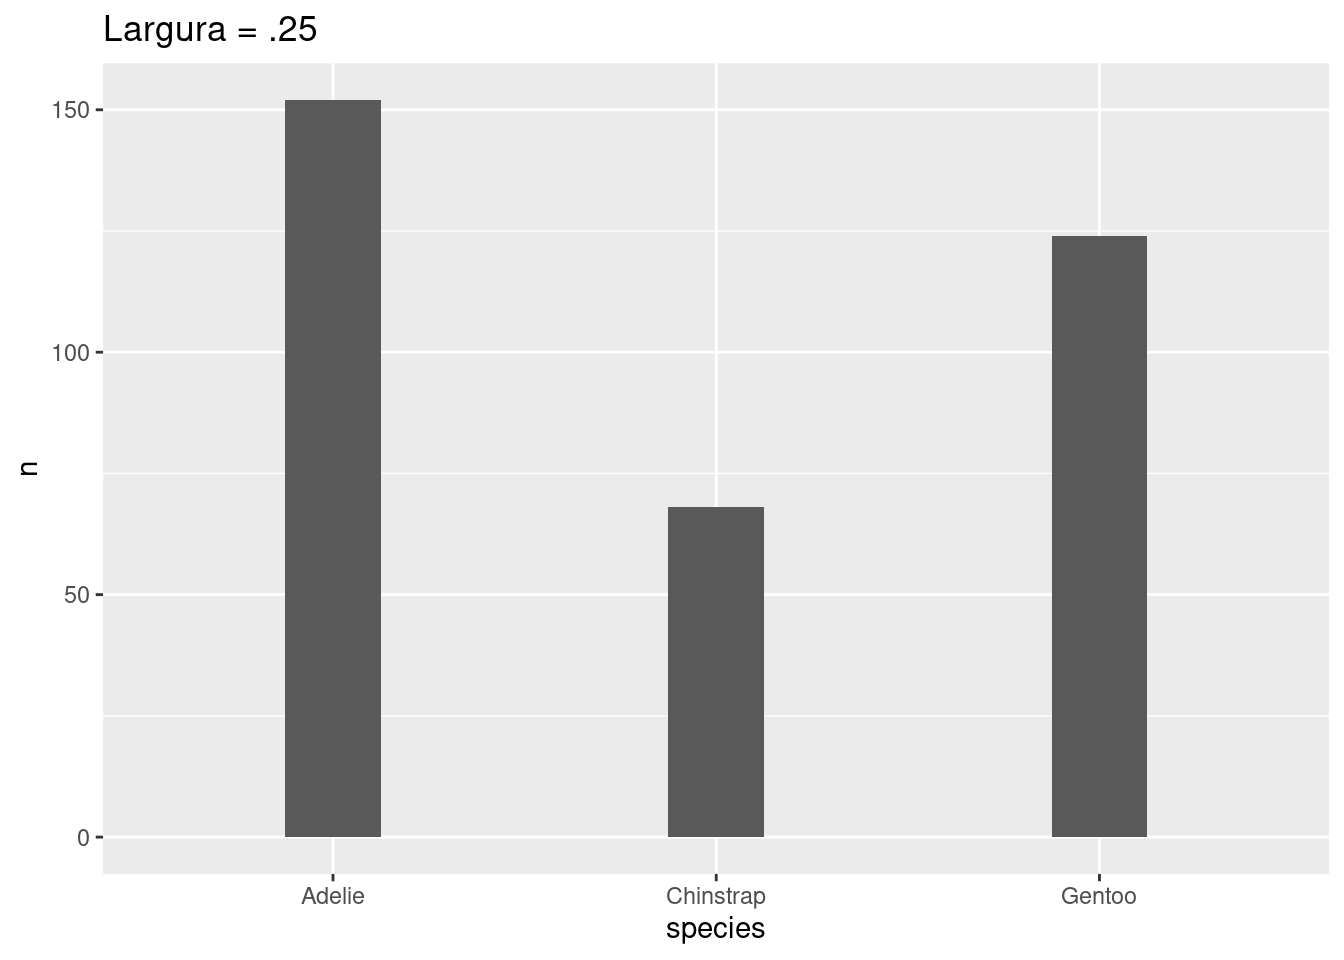
\includegraphics[width=0.7\linewidth]{livro_files/figure-latex/unnamed-chunk-204-2} \end{center}

Outra alternativa para os gráficos do tipo boxplot é utilizar o argumento \textbf{notch = TRUE} para produzir diagramas de caixa entalhados (notched). Estes diagramas são úteis para inferir de forma aproximada se exite diferença significativa entre as medias dos grupos.

\begin{Shaded}
\begin{Highlighting}[]
\FunctionTok{ggplot}\NormalTok{(penguins, }\FunctionTok{aes}\NormalTok{(}\AttributeTok{y =}\NormalTok{ flipper\_length\_mm, }\AttributeTok{x =}\NormalTok{ species)) }\SpecialCharTok{+}
  \FunctionTok{geom\_boxplot}\NormalTok{(}\AttributeTok{notch =} \ConstantTok{TRUE}\NormalTok{)}
\end{Highlighting}
\end{Shaded}

\begin{center}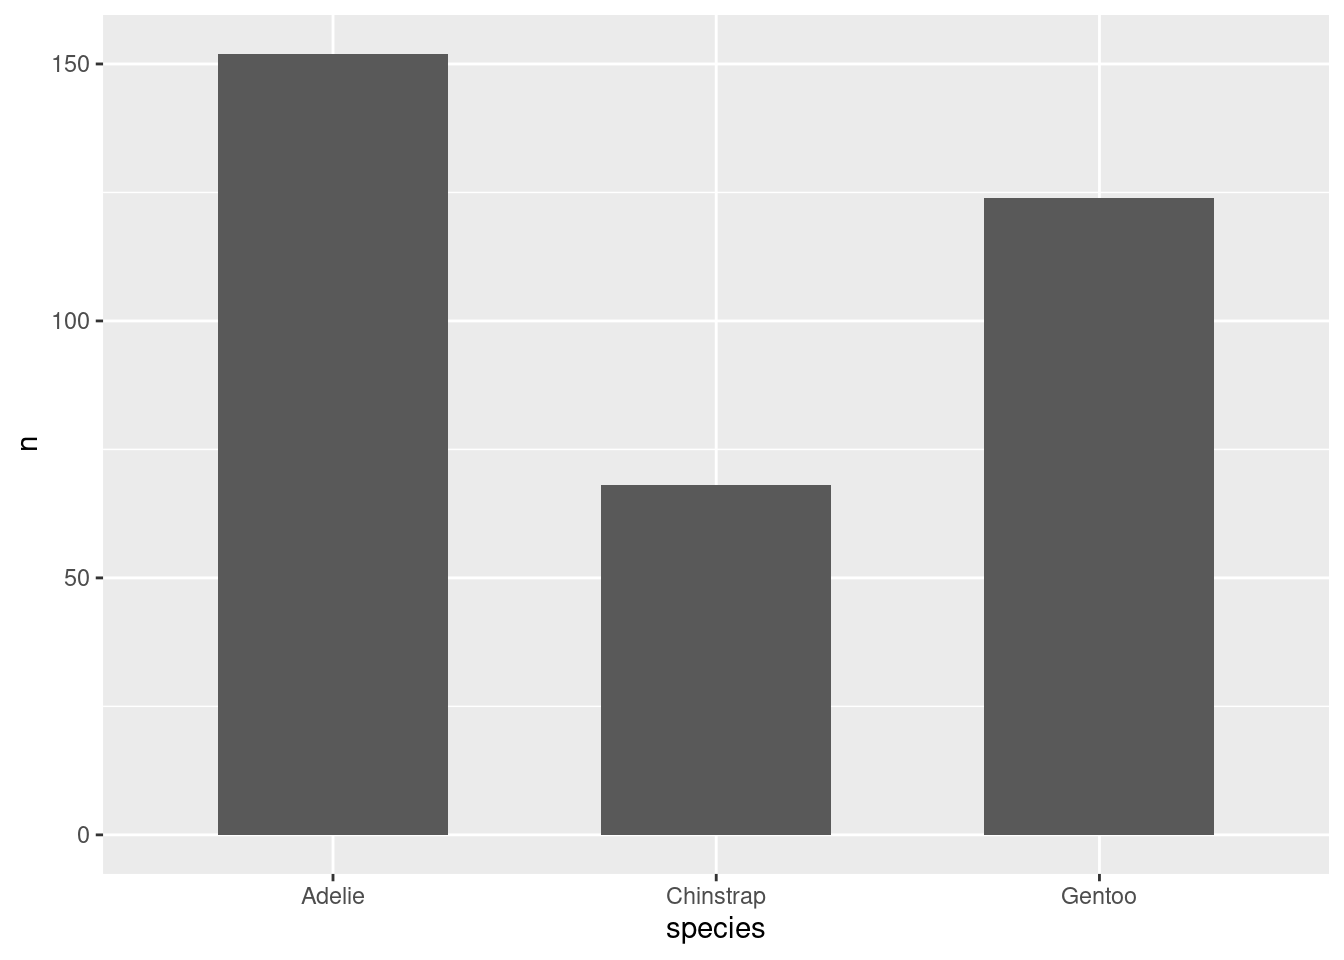
\includegraphics[width=0.7\linewidth]{livro_files/figure-latex/unnamed-chunk-205-1} \end{center}

\hypertarget{comparando-muxfaltiplas-categorias-3}{%
\subsubsection{4.6.2. Comparando múltiplas categorias}\label{comparando-muxfaltiplas-categorias-3}}

No exemplo abaixo, utilizamos cores diferentes para ilustrar espécies diferentes através do argumento \textbf{fill = species}.

\begin{Shaded}
\begin{Highlighting}[]

\FunctionTok{ggplot}\NormalTok{(penguins, }
       \FunctionTok{aes}\NormalTok{(}\AttributeTok{y =}\NormalTok{ flipper\_length\_mm, }\AttributeTok{x =}\NormalTok{ species, }\AttributeTok{fill =}\NormalTok{ species)) }\SpecialCharTok{+}
  \FunctionTok{geom\_boxplot}\NormalTok{()}
\end{Highlighting}
\end{Shaded}

\begin{center}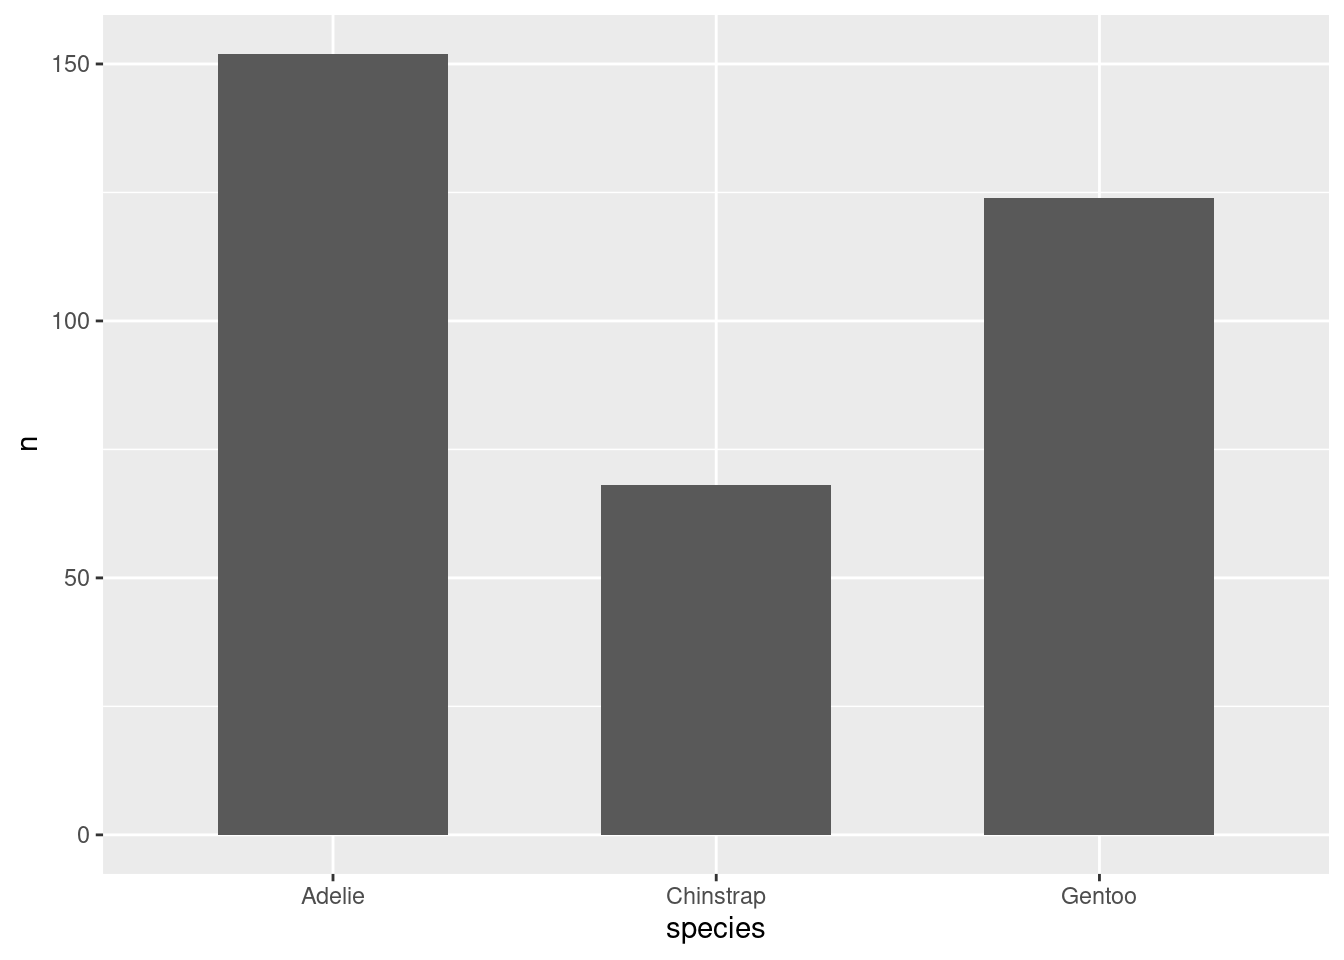
\includegraphics[width=0.7\linewidth]{livro_files/figure-latex/unnamed-chunk-206-1} \end{center}

\hypertarget{combinando-boxplot-com-pontos-jitter}{%
\subsubsection{\texorpdfstring{4.6.3. Combinando boxplot com pontos (\emph{jitter})}{4.6.3. Combinando boxplot com pontos (jitter)}}\label{combinando-boxplot-com-pontos-jitter}}

Podemos ainda acrescentar pontos para mostrar a distribuição dos dados.

\begin{Shaded}
\begin{Highlighting}[]
\CommentTok{\# boxplot com jitters}
\FunctionTok{ggplot}\NormalTok{(penguins, }
       \FunctionTok{aes}\NormalTok{(}\AttributeTok{y =}\NormalTok{ flipper\_length\_mm, }\AttributeTok{x =}\NormalTok{ species, }\AttributeTok{fill =}\NormalTok{ species)) }\SpecialCharTok{+}
  \FunctionTok{geom\_boxplot}\NormalTok{() }\SpecialCharTok{+}
  \FunctionTok{geom\_jitter}\NormalTok{(}\AttributeTok{size =}\NormalTok{ .}\DecValTok{6}\NormalTok{, }\AttributeTok{width =}\NormalTok{ .}\DecValTok{2}\NormalTok{)}
\end{Highlighting}
\end{Shaded}

\begin{center}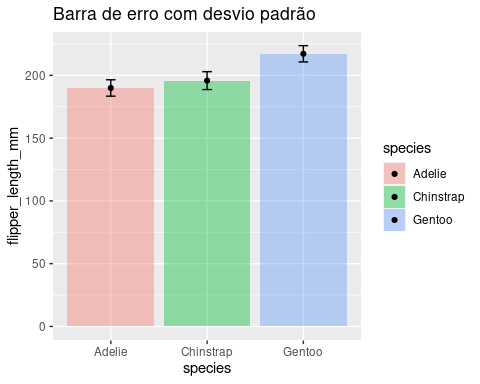
\includegraphics[width=0.7\linewidth]{livro_files/figure-latex/unnamed-chunk-207-1} \end{center}

\hypertarget{gruxe1fico-de-violino-violin-plot-como-alternativa-ao-boxplot}{%
\subsubsection{\texorpdfstring{4.6.4. Gráfico de violino (\emph{violin plot}) como alternativa ao boxplot}{4.6.4. Gráfico de violino (violin plot) como alternativa ao boxplot}}\label{gruxe1fico-de-violino-violin-plot-como-alternativa-ao-boxplot}}

Além das caixas, podemos utilizar o formato de ``violino'' para representar a variação de dados contínuos entre categorias. A informação adicional ao boxplot que o gráfico de violino permite visualizar é a densidade dos pontos, assim como apresentamos acima no gráfico de densidades \texttt{geom\_density()}. A diferença é que a densidade é espelhada e, desse modo, podemos visualizar os intervalores dos dados com maior ou menor concentração de valores.

\begin{Shaded}
\begin{Highlighting}[]
\CommentTok{\# violino com jitters}
\FunctionTok{ggplot}\NormalTok{(penguins, }\FunctionTok{aes}\NormalTok{(}\AttributeTok{y =}\NormalTok{ flipper\_length\_mm, }\AttributeTok{x =}\NormalTok{ species, }\AttributeTok{fill =}\NormalTok{ species)) }\SpecialCharTok{+}
  \FunctionTok{geom\_violin}\NormalTok{() }\SpecialCharTok{+}
  \FunctionTok{geom\_jitter}\NormalTok{(}\AttributeTok{size =}\NormalTok{ .}\DecValTok{6}\NormalTok{, }\AttributeTok{width =}\NormalTok{ .}\DecValTok{2}\NormalTok{)}
\end{Highlighting}
\end{Shaded}

\begin{center}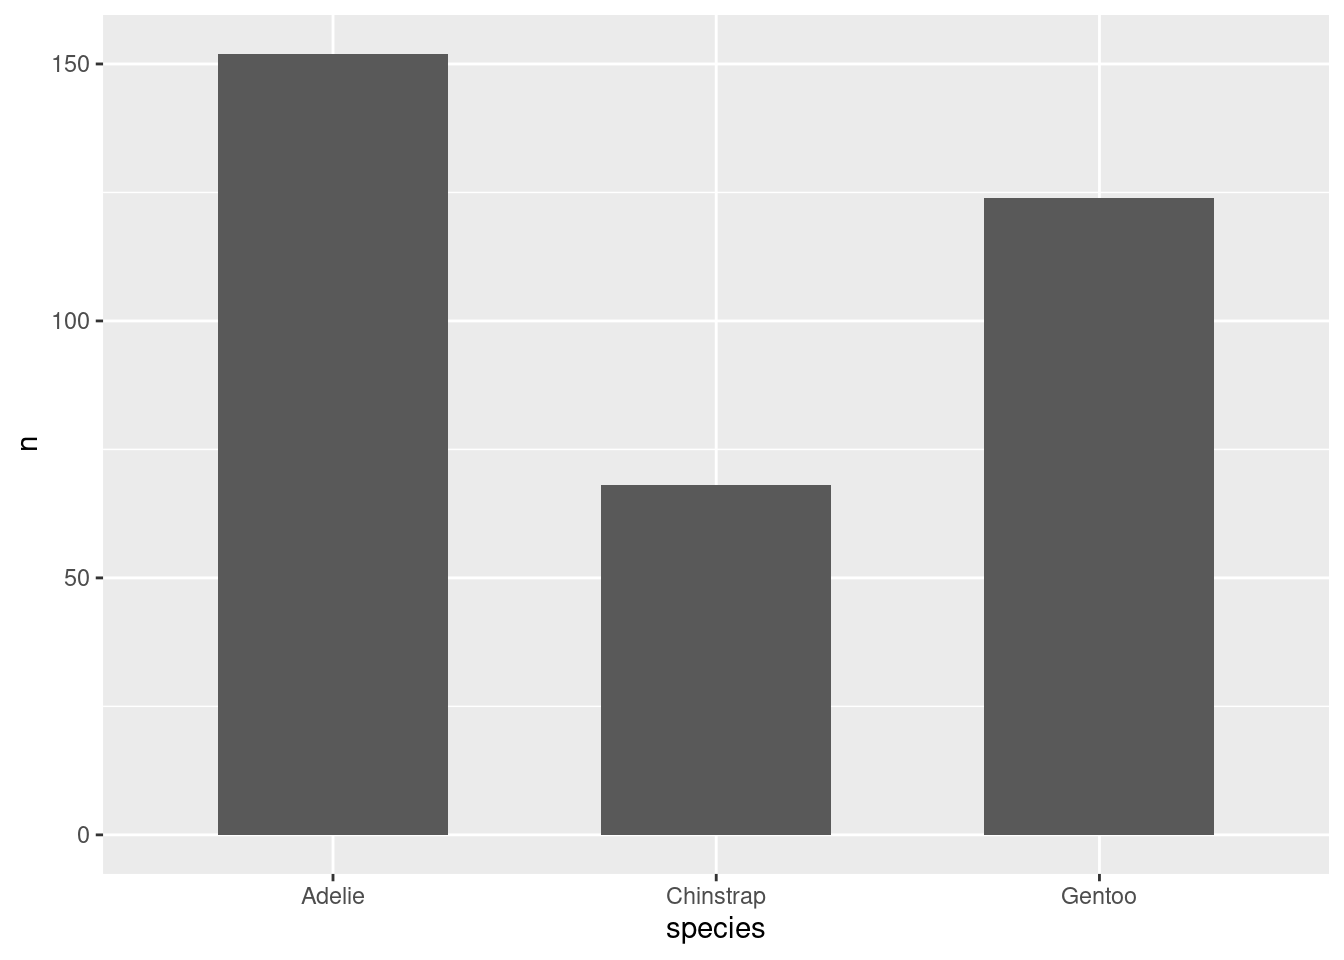
\includegraphics[width=0.7\linewidth]{livro_files/figure-latex/unnamed-chunk-208-1} \end{center}

É possível também combinar boxplot e gráfico de violino em um único gráfico.

\begin{Shaded}
\begin{Highlighting}[]
\CommentTok{\# violino com boxplot}
\FunctionTok{ggplot}\NormalTok{(penguins, }\FunctionTok{aes}\NormalTok{(}\AttributeTok{y =}\NormalTok{ flipper\_length\_mm, }\AttributeTok{x =}\NormalTok{ species, }\AttributeTok{fill =}\NormalTok{ species)) }\SpecialCharTok{+}
  \FunctionTok{geom\_violin}\NormalTok{() }\SpecialCharTok{+}
  \FunctionTok{geom\_boxplot}\NormalTok{(}\AttributeTok{width =} \FloatTok{0.1}\NormalTok{, }\AttributeTok{fill =} \StringTok{"grey"}\NormalTok{)}
\end{Highlighting}
\end{Shaded}

\begin{center}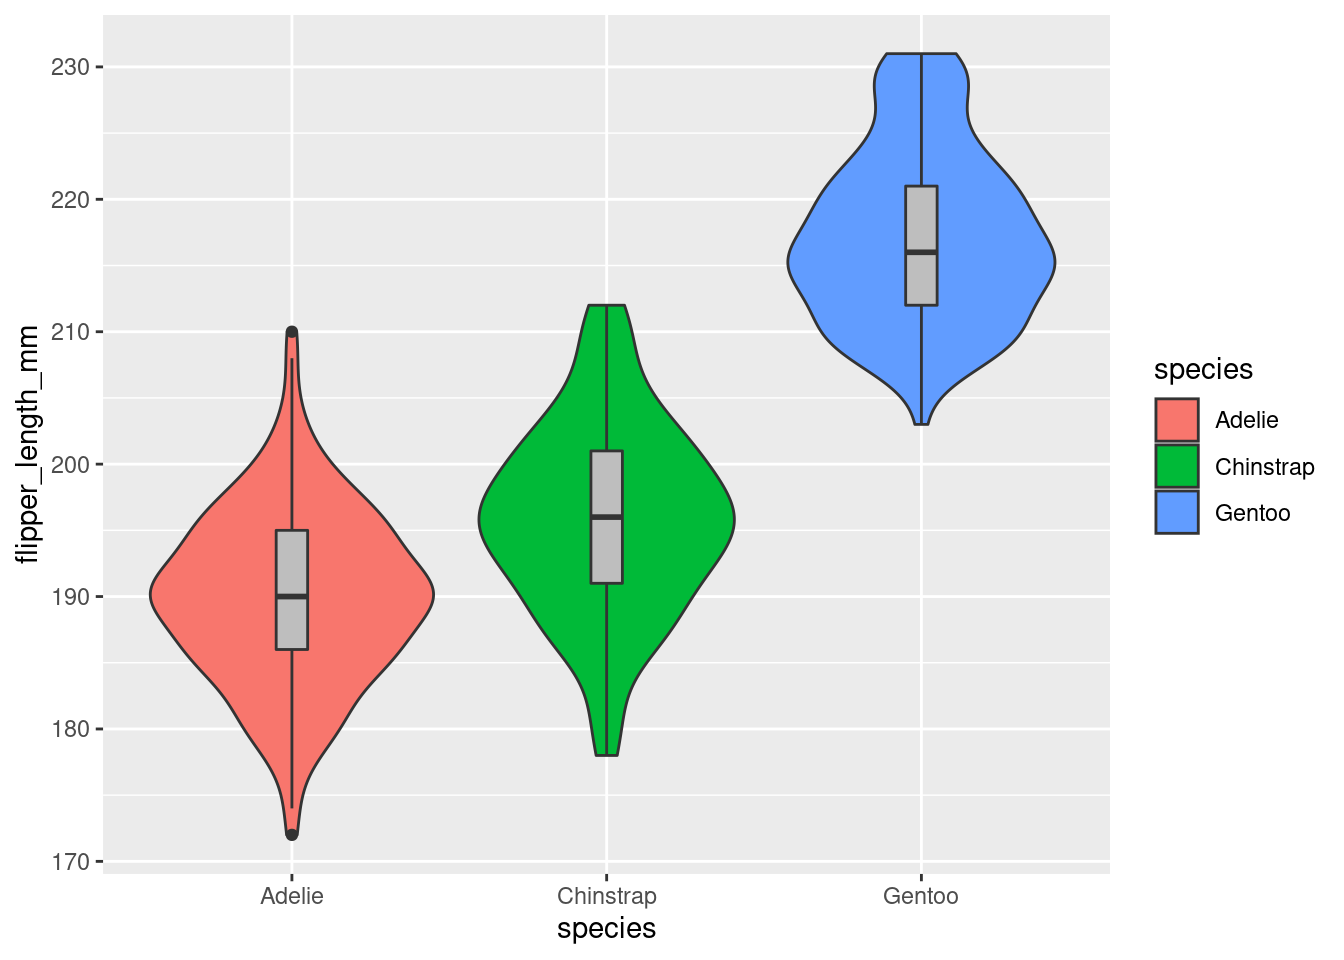
\includegraphics[width=0.7\linewidth]{livro_files/figure-latex/unnamed-chunk-209-1} \end{center}

\hypertarget{ajustes-finos-versuxe3o-personalizada-4}{%
\subsubsection{4.6.5. Ajustes finos (versão personalizada)}\label{ajustes-finos-versuxe3o-personalizada-4}}

\begin{Shaded}
\begin{Highlighting}[]

\DocumentationTok{\#\#\# geom\_boxplot()}

\FunctionTok{ggplot}\NormalTok{(}\AttributeTok{data =}\NormalTok{ penguins, }
       \FunctionTok{aes}\NormalTok{(}\AttributeTok{x =}\NormalTok{ species, }\AttributeTok{y =}\NormalTok{ flipper\_length\_mm, }\AttributeTok{fill =}\NormalTok{ species)) }\SpecialCharTok{+}
  \FunctionTok{geom\_boxplot}\NormalTok{(}\AttributeTok{width =}\NormalTok{ .}\DecValTok{3}\NormalTok{, }
               \AttributeTok{show.legend =} \ConstantTok{FALSE}\NormalTok{) }\SpecialCharTok{+}
  \FunctionTok{geom\_jitter}\NormalTok{(}\AttributeTok{alpha =}\NormalTok{ .}\DecValTok{5}\NormalTok{, }
              \AttributeTok{show.legend =} \ConstantTok{FALSE}\NormalTok{, }
              \AttributeTok{position =} \FunctionTok{position\_jitter}\NormalTok{(}\AttributeTok{width =}\NormalTok{ .}\DecValTok{1}\NormalTok{, }\AttributeTok{seed =} \DecValTok{0}\NormalTok{)) }\SpecialCharTok{+}
  \FunctionTok{scale\_fill\_manual}\NormalTok{(}\AttributeTok{values =} \FunctionTok{c}\NormalTok{(}\StringTok{"darkorange"}\NormalTok{, }\StringTok{"purple"}\NormalTok{, }\StringTok{"cyan4"}\NormalTok{)) }\SpecialCharTok{+}
  \FunctionTok{theme\_bw}\NormalTok{(}\AttributeTok{base\_size =} \DecValTok{16}\NormalTok{) }\SpecialCharTok{+}
  \FunctionTok{labs}\NormalTok{(}\AttributeTok{x =} \StringTok{"Species"}\NormalTok{, }\AttributeTok{y =} \StringTok{"Flipper length (mm)"}\NormalTok{)}


\CommentTok{\# geom\_violin()}
\FunctionTok{ggplot}\NormalTok{(}\AttributeTok{data =}\NormalTok{ penguins, }
       \FunctionTok{aes}\NormalTok{(}\AttributeTok{x =}\NormalTok{ species, }\AttributeTok{y =}\NormalTok{ flipper\_length\_mm, }\AttributeTok{fill =}\NormalTok{ species)) }\SpecialCharTok{+}
  \FunctionTok{geom\_violin}\NormalTok{(}\AttributeTok{width =}\NormalTok{ .}\DecValTok{3}\NormalTok{, }
              \AttributeTok{show.legend =} \ConstantTok{FALSE}\NormalTok{) }\SpecialCharTok{+}
  \FunctionTok{geom\_point}\NormalTok{(}\AttributeTok{alpha =}\NormalTok{ .}\DecValTok{5}\NormalTok{, }
              \AttributeTok{show.legend =} \ConstantTok{FALSE}\NormalTok{) }\SpecialCharTok{+}
  \FunctionTok{scale\_fill\_manual}\NormalTok{(}\AttributeTok{values =} \FunctionTok{c}\NormalTok{(}\StringTok{"darkorange"}\NormalTok{, }\StringTok{"purple"}\NormalTok{, }\StringTok{"cyan4"}\NormalTok{)) }\SpecialCharTok{+}
  \FunctionTok{theme\_bw}\NormalTok{(}\AttributeTok{base\_size =} \DecValTok{16}\NormalTok{) }\SpecialCharTok{+}
  \FunctionTok{labs}\NormalTok{(}\AttributeTok{title =} \StringTok{"Pontos sem jitter"}\NormalTok{, }\AttributeTok{x =} \StringTok{"Species"}\NormalTok{, }\AttributeTok{y =} \StringTok{"Flipper length (mm)"}\NormalTok{)}

\CommentTok{\# geom\_violin()}
\FunctionTok{ggplot}\NormalTok{(}\AttributeTok{data =}\NormalTok{ penguins, }
       \FunctionTok{aes}\NormalTok{(}\AttributeTok{x =}\NormalTok{ species, }\AttributeTok{y =}\NormalTok{ flipper\_length\_mm, }\AttributeTok{fill =}\NormalTok{ species)) }\SpecialCharTok{+}
  \FunctionTok{geom\_violin}\NormalTok{(}\AttributeTok{width =}\NormalTok{ .}\DecValTok{3}\NormalTok{, }
              \AttributeTok{show.legend =} \ConstantTok{FALSE}\NormalTok{) }\SpecialCharTok{+}
  \FunctionTok{geom\_jitter}\NormalTok{(}\AttributeTok{alpha =}\NormalTok{ .}\DecValTok{5}\NormalTok{, }
              \AttributeTok{show.legend =} \ConstantTok{FALSE}\NormalTok{, }
              \AttributeTok{position =} \FunctionTok{position\_jitter}\NormalTok{(}\AttributeTok{width =}\NormalTok{ .}\DecValTok{1}\NormalTok{, }\AttributeTok{seed =} \DecValTok{0}\NormalTok{)) }\SpecialCharTok{+}
  \FunctionTok{scale\_fill\_manual}\NormalTok{(}\AttributeTok{values =} \FunctionTok{c}\NormalTok{(}\StringTok{"darkorange"}\NormalTok{, }\StringTok{"purple"}\NormalTok{, }\StringTok{"cyan4"}\NormalTok{)) }\SpecialCharTok{+}
  \FunctionTok{theme\_bw}\NormalTok{(}\AttributeTok{base\_size =} \DecValTok{16}\NormalTok{) }\SpecialCharTok{+}
  \FunctionTok{labs}\NormalTok{(}\AttributeTok{title =} \StringTok{"Pontos com jitter"}\NormalTok{,, }\AttributeTok{x =} \StringTok{"Species"}\NormalTok{, }\AttributeTok{y =} \StringTok{"Flipper length (mm)"}\NormalTok{)}
\end{Highlighting}
\end{Shaded}

\begin{center}\includegraphics[width=0.7\linewidth]{livro_files/figure-latex/unnamed-chunk-210-1} \includegraphics[width=0.7\linewidth]{livro_files/figure-latex/unnamed-chunk-210-2} \includegraphics[width=0.7\linewidth]{livro_files/figure-latex/unnamed-chunk-210-3} \end{center}

\hypertarget{principais-camadas-utilizadas-no-geom_boxplote-geom_violin}{%
\subsubsection{\texorpdfstring{4.6.6. Principais camadas utilizadas no \texttt{geom\_boxplot()}e \texttt{geom\_violin()}}{4.6.6. Principais camadas utilizadas no geom\_boxplot()e geom\_violin()}}\label{principais-camadas-utilizadas-no-geom_boxplote-geom_violin}}

\begin{itemize}
\item
  \texttt{aes()}:

  \begin{itemize}
  \item
    Eixo X: variável categórica (\emph{species})
  \item
    Eixo Y: variável contínua (\emph{flipper\_length\_mm})
  \item
    Preenchimento (\emph{fill}): a variável categórica (\emph{species}) define a cor do preenchimento e os níveis dentro desta categoria determinam o número de cores que devem ser indicadas no \texttt{scale\_fill\_manual()}.
  \end{itemize}
\item
  \texttt{geom():}

  \begin{itemize}
  \item
    \texttt{geom\_boxplot()}

    \begin{itemize}
    \item
      \texttt{width}: largura das barras (valor padrão: width = 1)
    \item
      \texttt{fill}: pode definir uma cor padrão (caso não tenha utilizado o fill dentro do argumento \texttt{aes()}) como \texttt{fill\ =\ "grey"}
    \item
      \texttt{notch}: a escolha padrão da função \texttt{geom\_boxplot()} é \texttt{notch\ =\ FALSE}; para utilizar a caixa entalhada o argumento deve ser \texttt{notch\ =\ TRUE}
    \end{itemize}
  \item
    \texttt{geom\_violin()}

    \begin{itemize}
    \tightlist
    \item
      assim como nas outras formas geométricas, é possível controlar largura, cor, preenchimento e transparências dos violinos
    \end{itemize}
  \item
    \texttt{geom\_jitter()}

    \begin{itemize}
    \tightlist
    \item
      esta função basicamente ``agita'' aleatóriamente os pontos para evitar a sobreposição de valores idênticos. Esta função produz a mesma representação se usar a função \texttt{geom\_point(position\ =\ "jitter")}
    \end{itemize}
  \end{itemize}
\item
  \texttt{scale()}:

  \begin{itemize}
  \tightlist
  \item
    \texttt{scale\_fill\_manual()} para definir manualmente as cores de preferência do usuário
  \end{itemize}
\item
  \texttt{theme()}: \texttt{theme\_bw()}para selecionar o tema com fundo branco e \texttt{labs()} para personalizar o títulos dos eixos X e Y, e da legenda.
\end{itemize}

\hypertarget{gruxe1fico-de-dispersuxe3o-scatter-plot}{%
\section{\texorpdfstring{4.7. Gráfico de dispersão (\emph{scatter plot})}{4.7. Gráfico de dispersão (scatter plot)}}\label{gruxe1fico-de-dispersuxe3o-scatter-plot}}

O \href{https://pt.wikipedia.org/wiki/Gr\%C3\%A1fico_de_barras}{gráfico de dispersão} (em ingl\textasciitilde es, \emph{scatterplot}) é famoso na ecologia por ser a visualização preferida para prepresentar a relação entre área e riqueza de espécies. Neste gráfico, os eixos X e Y são representados por variáveis contínuas. Em especial, os gráficos de dispersão são usados para representar os resultados testados por análises estatísticas como regressão linear, ancova, mantel, PCA, PCoA, entre outros (\textbf{Capítulos 7-14,} ).

\hypertarget{versuxe3o-padruxe3o-5}{%
\subsection{4.7.1. Versão padrão}\label{versuxe3o-padruxe3o-5}}

\begin{Shaded}
\begin{Highlighting}[]

\FunctionTok{ggplot}\NormalTok{(penguins, }
       \FunctionTok{aes}\NormalTok{(}\AttributeTok{x =}\NormalTok{ bill\_length\_mm, }\AttributeTok{y =}\NormalTok{ bill\_depth\_mm)) }\SpecialCharTok{+}
  \FunctionTok{geom\_point}\NormalTok{()}
\end{Highlighting}
\end{Shaded}

\begin{center}\includegraphics[width=0.7\linewidth]{livro_files/figure-latex/unnamed-chunk-211-1} \end{center}

\hypertarget{definindo-a-cor-tamanho-forma-e-preenchimento-dos-pontos}{%
\subsection{4.7.2. Definindo a cor, tamanho, forma e preenchimento dos pontos}\label{definindo-a-cor-tamanho-forma-e-preenchimento-dos-pontos}}

\begin{Shaded}
\begin{Highlighting}[]
\CommentTok{\# Cor e tamanho dos pontos }
\FunctionTok{ggplot}\NormalTok{(penguins, }
       \FunctionTok{aes}\NormalTok{(}\AttributeTok{x =}\NormalTok{ bill\_length\_mm, }\AttributeTok{y =}\NormalTok{ bill\_depth\_mm)) }\SpecialCharTok{+}
  \FunctionTok{geom\_point}\NormalTok{(}\AttributeTok{color =} \StringTok{"royalblue"}\NormalTok{,}
             \AttributeTok{size =} \DecValTok{3}\NormalTok{)}\SpecialCharTok{+}
\FunctionTok{labs}\NormalTok{(}\AttributeTok{title =} \StringTok{"Sem transparência"}\NormalTok{)}

\CommentTok{\# Cor e tamanho dos pontos }
\FunctionTok{ggplot}\NormalTok{(penguins, }
       \FunctionTok{aes}\NormalTok{(}\AttributeTok{x =}\NormalTok{ bill\_length\_mm, }\AttributeTok{y =}\NormalTok{ bill\_depth\_mm)) }\SpecialCharTok{+}
  \FunctionTok{geom\_point}\NormalTok{(}\AttributeTok{color =} \StringTok{"red"}\NormalTok{,}
             \AttributeTok{size =} \DecValTok{4}\NormalTok{,}
             \AttributeTok{alpha =} \FloatTok{0.5}\NormalTok{)}\SpecialCharTok{+}
\FunctionTok{labs}\NormalTok{(}\AttributeTok{title =} \StringTok{"Com transparência"}\NormalTok{)}
\end{Highlighting}
\end{Shaded}

\begin{center}\includegraphics[width=0.7\linewidth]{livro_files/figure-latex/unnamed-chunk-212-1} \includegraphics[width=0.7\linewidth]{livro_files/figure-latex/unnamed-chunk-212-2} \end{center}

A forma dos pontos permite dois controles importantes: a forma em si (símbolos como círculo, quadrado, etc.) e a possibilidade de preenchimento da forma. A figura a seguir discrimina esses símbolos e o valor que deve ser utilizado para desenhar a forma preferida. É importante notar que os símbolos 21 a 25 possuem dois argumentos: (i) cor (que, na verdade, é a cor da linha do símbolo) e (ii) fill (cor que define o preenchimento do símbolo). O tipo de símbolo é definido pelo argumento \textbf{\texttt{shape}}.

\begin{figure}

{\centering \includegraphics[width=0.5\linewidth]{img/cap06_fig02} 

}

\caption{Figura 3. Tipos de símbolos disponíveis.}\label{fig:fig-point-shape}
\end{figure}

Assim, é possível controlar cores, formas e preenchimento combinado os argumentos \texttt{shape}, \texttt{fill}e \texttt{color}com a função \texttt{scale\_manual()}. É importante notar que para os símbolos entre 15 e 20 só podemos controlar o argumento cor, enquanto os símbolos entre 21 e 25 podemos controlar a cor e o preenchimento.

\begin{Shaded}
\begin{Highlighting}[]

\CommentTok{\# shape = 1 e size = 2}
\FunctionTok{ggplot}\NormalTok{(penguins, }\FunctionTok{aes}\NormalTok{(}\AttributeTok{x =}\NormalTok{ bill\_length\_mm, }\AttributeTok{y =}\NormalTok{ bill\_depth\_mm)) }\SpecialCharTok{+}
  \FunctionTok{geom\_point}\NormalTok{(}\AttributeTok{shape =} \DecValTok{1}\NormalTok{, }\AttributeTok{size =} \DecValTok{2}\NormalTok{)}

\CommentTok{\# shape = 19 (símbolo padrão da função) e size = 3}
\FunctionTok{ggplot}\NormalTok{(penguins, }
       \FunctionTok{aes}\NormalTok{(}\AttributeTok{x =}\NormalTok{ bill\_length\_mm, }\AttributeTok{y =}\NormalTok{ bill\_depth\_mm, }\AttributeTok{color =}\NormalTok{ species)) }\SpecialCharTok{+}
  \FunctionTok{geom\_point}\NormalTok{(}\AttributeTok{shape =} \DecValTok{19}\NormalTok{, }\AttributeTok{size =} \DecValTok{3}\NormalTok{)}

\CommentTok{\# shape = 21 e size = 4}
\FunctionTok{ggplot}\NormalTok{(penguins, }
       \FunctionTok{aes}\NormalTok{(}\AttributeTok{x =}\NormalTok{ bill\_length\_mm, }\AttributeTok{y =}\NormalTok{ bill\_depth\_mm, }\AttributeTok{fill =}\NormalTok{ species)) }\SpecialCharTok{+}
  \FunctionTok{geom\_point}\NormalTok{(}\AttributeTok{shape =} \DecValTok{21}\NormalTok{, }\AttributeTok{size =} \DecValTok{4}\NormalTok{, }\AttributeTok{color =} \StringTok{"black"}\NormalTok{)}
\end{Highlighting}
\end{Shaded}

\begin{center}\includegraphics[width=0.5\linewidth]{livro_files/figure-latex/unnamed-chunk-213-1} \includegraphics[width=0.5\linewidth]{livro_files/figure-latex/unnamed-chunk-213-2} \includegraphics[width=0.5\linewidth]{livro_files/figure-latex/unnamed-chunk-213-3} \end{center}

\hypertarget{definindo-linhas-de-ajuste}{%
\subsection{4.7.3. Definindo linhas de ajuste}\label{definindo-linhas-de-ajuste}}

Quando usamos modelos estatísticos como, por exemplo, lm(), glm(), gam(), entre outros, podemos utilizar os valores preditos para demonstrar a relação entre as variáveis X e Y. No ggplot2 a função \texttt{geom\_smooth()} faz esse ajuste com certa simplicidade. Além disso, incluir a cor da espécie dentro do \texttt{aes()} essa informação é herdada para as próximas camadas. Neste caso, uma regressão linear é plotada para o subconjunto de dados que representa cada espécie.

\begin{Shaded}
\begin{Highlighting}[]

\CommentTok{\# shape = 21 e size = 4}
\FunctionTok{ggplot}\NormalTok{(penguins, }
       \FunctionTok{aes}\NormalTok{(}\AttributeTok{x =}\NormalTok{ bill\_length\_mm, }\AttributeTok{y =}\NormalTok{ bill\_depth\_mm, }\AttributeTok{color =}\NormalTok{ species)) }\SpecialCharTok{+}
  \FunctionTok{geom\_point}\NormalTok{(}\AttributeTok{size =} \DecValTok{4}\NormalTok{, }\AttributeTok{alpha =}\NormalTok{ .}\DecValTok{5}\NormalTok{)}\SpecialCharTok{+}
  \FunctionTok{geom\_smooth}\NormalTok{(}\AttributeTok{method=}\NormalTok{ lm)}
\end{Highlighting}
\end{Shaded}

\begin{center}\includegraphics[width=0.5\linewidth]{livro_files/figure-latex/unnamed-chunk-214-1} \end{center}

\hypertarget{ajustes-finos-versuxe3o-personalizada-5}{%
\subsection{4.7.4. Ajustes finos (versão personalizada)}\label{ajustes-finos-versuxe3o-personalizada-5}}

\begin{Shaded}
\begin{Highlighting}[]

\FunctionTok{ggplot}\NormalTok{(}\AttributeTok{data =}\NormalTok{ penguins, }
       \FunctionTok{aes}\NormalTok{(}\AttributeTok{x =}\NormalTok{ bill\_length\_mm, }
           \AttributeTok{y =}\NormalTok{ bill\_depth\_mm,}
           \AttributeTok{color =}\NormalTok{ species,}
           \AttributeTok{shape =}\NormalTok{ species)) }\SpecialCharTok{+}
  \FunctionTok{geom\_point}\NormalTok{(}\AttributeTok{size =} \DecValTok{3}\NormalTok{, }
             \AttributeTok{alpha =} \FloatTok{0.8}\NormalTok{) }\SpecialCharTok{+}
  \FunctionTok{geom\_smooth}\NormalTok{(}\AttributeTok{method =} \StringTok{"lm"}\NormalTok{, }\AttributeTok{se =} \ConstantTok{FALSE}\NormalTok{) }\SpecialCharTok{+}
  \FunctionTok{scale\_shape\_manual}\NormalTok{(}\AttributeTok{values =} \FunctionTok{c}\NormalTok{(}\DecValTok{19}\NormalTok{, }\DecValTok{15}\NormalTok{, }\DecValTok{17}\NormalTok{))}\SpecialCharTok{+}
  \FunctionTok{scale\_color\_manual}\NormalTok{(}\AttributeTok{values =} \FunctionTok{c}\NormalTok{(}\StringTok{"darkorange"}\NormalTok{, }\StringTok{"purple"}\NormalTok{, }\StringTok{"cyan4"}\NormalTok{)) }\SpecialCharTok{+}
  \FunctionTok{theme\_bw}\NormalTok{(}\AttributeTok{base\_size =} \DecValTok{16}\NormalTok{) }\SpecialCharTok{+}
  \FunctionTok{labs}\NormalTok{(}\AttributeTok{x =} \StringTok{"Comprimento do bico (mm)"}\NormalTok{, }\AttributeTok{y =} \StringTok{"Profundidade do bico (mm)"}\NormalTok{, }
       \AttributeTok{color =} \StringTok{"Espécies"}\NormalTok{, }\AttributeTok{shape =} \StringTok{"Espécies"}\NormalTok{)}
\end{Highlighting}
\end{Shaded}

\begin{center}\includegraphics[width=0.7\linewidth]{livro_files/figure-latex/unnamed-chunk-215-1} \end{center}

Além disso, podemos relacionar dados não tão usuais. Recomendamos a leitura do artigo de Matejka \& Fitzmaurice (2017) que apresenta as armadilhas típicas que dados podem gerar quando evitamos de visualizá-los previmamente.

\begin{Shaded}
\begin{Highlighting}[]

\CommentTok{\# data + plot}
\NormalTok{datasaurus\_dozen }\SpecialCharTok{\%\textgreater{}\%} 
\NormalTok{    dplyr}\SpecialCharTok{::}\FunctionTok{filter}\NormalTok{(dataset }\SpecialCharTok{==} \StringTok{"dino"}\NormalTok{) }\SpecialCharTok{\%\textgreater{}\%} 
    \FunctionTok{ggplot}\NormalTok{() }\SpecialCharTok{+}
    \FunctionTok{aes}\NormalTok{(}\AttributeTok{x =}\NormalTok{ x, }\AttributeTok{y =}\NormalTok{ y) }\SpecialCharTok{+}
    \FunctionTok{geom\_point}\NormalTok{(}\AttributeTok{colour =} \StringTok{"black"}\NormalTok{, }\AttributeTok{fill =} \StringTok{"black"}\NormalTok{, }
               \AttributeTok{size =} \DecValTok{5}\NormalTok{, }\AttributeTok{alpha =}\NormalTok{ .}\DecValTok{75}\NormalTok{, }\AttributeTok{pch =} \DecValTok{21}\NormalTok{) }\SpecialCharTok{+}
    \FunctionTok{theme\_bw}\NormalTok{() }\SpecialCharTok{+}
    \FunctionTok{theme}\NormalTok{(}\AttributeTok{axis.title =} \FunctionTok{element\_text}\NormalTok{(}\AttributeTok{size =} \DecValTok{24}\NormalTok{),}
        \AttributeTok{axis.text.x =} \FunctionTok{element\_text}\NormalTok{(}\AttributeTok{size =} \DecValTok{20}\NormalTok{),}
        \AttributeTok{axis.text.y =} \FunctionTok{element\_text}\NormalTok{(}\AttributeTok{size =} \DecValTok{20}\NormalTok{))}
\end{Highlighting}
\end{Shaded}

\begin{center}\includegraphics[width=0.7\linewidth]{livro_files/figure-latex/unnamed-chunk-216-1} \end{center}

\hypertarget{visualizauxe7uxe3o-de-muxfaltiplos-gruxe1ficos-pareados}{%
\section{4.8. Visualização de múltiplos gráficos pareados}\label{visualizauxe7uxe3o-de-muxfaltiplos-gruxe1ficos-pareados}}

Muitas vezes precisamos compreender a correlação entre múltiplas variáveis, sendo comuum que essas variáveis sejam de mais de um tipo (contínua, categórica, etc). A solução mais indicada para termos uma visão geral do conjunto de dados e de suas interrelações é o gráfico generalizado pareado (\href{https://www.tandfonline.com/doi/full/10.1080/10618600.2012.694762}{Emerson et al. 2013}).

\hypertarget{gruxe1fico-pareado-com-variuxe1veis-contuxednuas}{%
\subsection{4.8.1. Gráfico pareado com variáveis contínuas}\label{gruxe1fico-pareado-com-variuxe1veis-contuxednuas}}

A função \texttt{ggpairs()}do pacote GGally permite criar múltiplos gráficos pareados comparando as variáveis contínuas no seu conjunto de dados. Além de plotar gráficos de dispersão de cada par de variáveis, ela apresenta gráficos de densidade de cada variável individualmente e, além disso, os valores de correlação entre os pares analisados com ou sem uma potencial variável categórica (neste caso, \emph{species})

\begin{Shaded}
\begin{Highlighting}[]

\NormalTok{penguins }\SpecialCharTok{\%\textgreater{}\%}
\NormalTok{  dplyr}\SpecialCharTok{::}\FunctionTok{select}\NormalTok{(body\_mass\_g, }\FunctionTok{ends\_with}\NormalTok{(}\StringTok{"\_mm"}\NormalTok{)) }\SpecialCharTok{\%\textgreater{}\%}
\NormalTok{  GGally}\SpecialCharTok{::}\FunctionTok{ggpairs}\NormalTok{(}\FunctionTok{aes}\NormalTok{(}\AttributeTok{color =}\NormalTok{ penguins}\SpecialCharTok{$}\NormalTok{species)) }\SpecialCharTok{+}
  \FunctionTok{scale\_colour\_manual}\NormalTok{(}\AttributeTok{values =} \FunctionTok{c}\NormalTok{(}\StringTok{"darkorange"}\NormalTok{, }\StringTok{"purple"}\NormalTok{, }\StringTok{"cyan4"}\NormalTok{)) }\SpecialCharTok{+}
  \FunctionTok{scale\_fill\_manual}\NormalTok{(}\AttributeTok{values =} \FunctionTok{c}\NormalTok{(}\StringTok{"darkorange"}\NormalTok{, }\StringTok{"purple"}\NormalTok{, }\StringTok{"cyan4"}\NormalTok{)) }\SpecialCharTok{+}
  \FunctionTok{theme\_bw}\NormalTok{()}
\end{Highlighting}
\end{Shaded}

\begin{center}\includegraphics[width=1\linewidth,height=1\textheight]{livro_files/figure-latex/unnamed-chunk-217-1} \end{center}

\hypertarget{gruxe1fico-pareado-com-vuxe1rios-tipos-de-variuxe1veis}{%
\subsection{4.8.2. Gráfico pareado com vários tipos de variáveis}\label{gruxe1fico-pareado-com-vuxe1rios-tipos-de-variuxe1veis}}

Como alternativa, a função \textbf{\texttt{ggpairs()}} permite também incluir variáveis categóricas nas comparações. Neste caso, ela reconhece o tipo de gráfico (boxplot, dispersão, etc\ldots) a partir da classe das variáveis.

\begin{Shaded}
\begin{Highlighting}[]
\NormalTok{penguins }\SpecialCharTok{\%\textgreater{}\%}
\NormalTok{  dplyr}\SpecialCharTok{::}\FunctionTok{select}\NormalTok{(species, sex, body\_mass\_g, }\FunctionTok{ends\_with}\NormalTok{(}\StringTok{"\_mm"}\NormalTok{)) }\SpecialCharTok{\%\textgreater{}\%}
\NormalTok{  GGally}\SpecialCharTok{::}\FunctionTok{ggpairs}\NormalTok{(}\FunctionTok{aes}\NormalTok{(}\AttributeTok{color =}\NormalTok{ species)) }\SpecialCharTok{+}
  \FunctionTok{scale\_colour\_manual}\NormalTok{(}\AttributeTok{values =} \FunctionTok{c}\NormalTok{(}\StringTok{"darkorange"}\NormalTok{, }\StringTok{"purple"}\NormalTok{, }\StringTok{"cyan4"}\NormalTok{)) }\SpecialCharTok{+}
  \FunctionTok{scale\_fill\_manual}\NormalTok{(}\AttributeTok{values =} \FunctionTok{c}\NormalTok{(}\StringTok{"darkorange"}\NormalTok{, }\StringTok{"purple"}\NormalTok{, }\StringTok{"cyan4"}\NormalTok{)) }\SpecialCharTok{+}
  \FunctionTok{theme\_bw}\NormalTok{()}
\end{Highlighting}
\end{Shaded}

\begin{center}\includegraphics[width=1\linewidth]{livro_files/figure-latex/unnamed-chunk-218-1} \end{center}

\hypertarget{erros-comuns-dos-usuuxe1rios-do-ggplot2-e-como-evituxe1-los}{%
\section{\texorpdfstring{5. Erros comuns dos usuários do \texttt{ggplot2} e como evitá-los}{5. Erros comuns dos usuários do ggplot2 e como evitá-los}}\label{erros-comuns-dos-usuuxe1rios-do-ggplot2-e-como-evituxe1-los}}

Abaixo, apresentamos uma lista não exaustiva dos erros mais comuns que cometemos (e vimos muitos usuários cometerem) ao fazer gráficos no ggplot2:

\begin{itemize}
\item
  Utilizar ajuste manual nas funções \texttt{scale\_shape\_manual()}, \texttt{scale\_color\_manual()} ou \texttt{scale\_fill\_manual()} sem indicar no argumento \texttt{aes()} as variáveis que devem definir cada um desses elementos gráficos.
\item
  Definir a cor ou preenchimento de um geom dentro do \texttt{aes()} global (\texttt{ggplot(aes(color\ =\ "black¨})) quando no fundo essa definição deveria ser dento do geom (\texttt{geom\_point(color\ =\ "black")}.
\item
  Utilizar ajuste manual na função \texttt{scale\_size\_manual()} indicando uma variável categórica ao invés de numérica.
\item
  Número de cores indicadas como valores no \textbf{\texttt{scale\_fill\_manual()}} ou \textbf{\texttt{scale\_color\_manual()}}: ao definir as cores de maneira personalizada (ou seja, não usando o padrão da função) é muito comum utilizarmos o número de cores usados por algum tutorial ou livro. Com frequência, o exemplo seguido e seus dados não possuem o mesmo número de cores. Deste modo, você pode usar comando no R para ajudar a quantificar o número de cores necessárias. Por exemplo, para os dados penguins, o comando a seguir indica o número de cores necessárias: \texttt{length(levels(penguins\$species))}. Assim, será necessário indicar três cores diferentes dentro da função \texttt{scale\_()}.
\item
  Função \texttt{geom\_smooth()}: como falado acima, a função \texttt{geom\_smooth()} é muito útil (e simples) para gerar as linhas de ajuste (best fit) típicas de modelos lineares e não lineares. Porém, fique alerta que ao usar, por exemplo, \texttt{geom\_smooth(method\ =\ lm)}, o modelo linear utilizado para testar sua predição foi o \texttt{lm()}. Se tiver utilizado \texttt{glm()}ou \texttt{gam()} o ajuste deve ser produzido a partir desses modelos.
\item
  Uso incorreto da classe das variáveis: neste caso, o usuário utilizar uma variável numérica (por exemplo, 1, 2 e 3) como variável categórica. Neste caso, é preciso transformar a variável numérica em variável categóricas (antes de fazer o ggplot2 ou dentro do \texttt{aes()}). Veja exemplos abaixo:
\end{itemize}

\begin{Shaded}
\begin{Highlighting}[]
\NormalTok{penguins }\SpecialCharTok{\%\textgreater{}\%}
  \FunctionTok{ggplot}\NormalTok{(}\FunctionTok{aes}\NormalTok{(}\AttributeTok{x =}\NormalTok{ year, }\AttributeTok{y =}\NormalTok{ bill\_length\_mm))}\SpecialCharTok{+}
  \FunctionTok{geom\_boxplot}\NormalTok{() }\SpecialCharTok{+} 
  \FunctionTok{theme\_bw}\NormalTok{()}\SpecialCharTok{+}
  \FunctionTok{labs}\NormalTok{(}\AttributeTok{title =} \StringTok{"Figura incorreta"}\NormalTok{)}

\NormalTok{penguins }\SpecialCharTok{\%\textgreater{}\%}
  \FunctionTok{ggplot}\NormalTok{(}\FunctionTok{aes}\NormalTok{(}\AttributeTok{x =} \FunctionTok{factor}\NormalTok{(year), }\AttributeTok{y =}\NormalTok{ bill\_length\_mm))}\SpecialCharTok{+}
  \FunctionTok{geom\_boxplot}\NormalTok{() }\SpecialCharTok{+} 
  \FunctionTok{theme\_bw}\NormalTok{()}\SpecialCharTok{+}
  \FunctionTok{labs}\NormalTok{(}\AttributeTok{title =} \StringTok{"Figura correta com transformação interna"}\NormalTok{)}

\NormalTok{penguins }\SpecialCharTok{\%\textgreater{}\%}
  \FunctionTok{mutate}\NormalTok{(}\AttributeTok{year\_f =} \FunctionTok{as.factor}\NormalTok{(year)) }\SpecialCharTok{\%\textgreater{}\%} 
  \FunctionTok{ggplot}\NormalTok{(}\FunctionTok{aes}\NormalTok{(}\AttributeTok{x =}\NormalTok{ year\_f, }\AttributeTok{y =}\NormalTok{ bill\_length\_mm))}\SpecialCharTok{+}
  \FunctionTok{geom\_boxplot}\NormalTok{() }\SpecialCharTok{+} 
  \FunctionTok{theme\_bw}\NormalTok{()}\SpecialCharTok{+}
  \FunctionTok{labs}\NormalTok{(}\AttributeTok{title =} \StringTok{"Figura correta com transformação prévia"}\NormalTok{)}
\end{Highlighting}
\end{Shaded}

\begin{center}\includegraphics[width=0.7\linewidth]{livro_files/figure-latex/unnamed-chunk-219-1} \includegraphics[width=0.7\linewidth]{livro_files/figure-latex/unnamed-chunk-219-2} \includegraphics[width=0.7\linewidth]{livro_files/figure-latex/unnamed-chunk-219-3} \end{center}

\hypertarget{finalizauxe7uxe3o-de-gruxe1ficos-para-publicauxe7uxe3o}{%
\section{6. Finalização de gráficos para publicação}\label{finalizauxe7uxe3o-de-gruxe1ficos-para-publicauxe7uxe3o}}

\hypertarget{posiuxe7uxe3o-cores-e-fonte-da-legenda}{%
\subsection{6.1. Posição, cores e fonte da legenda}\label{posiuxe7uxe3o-cores-e-fonte-da-legenda}}

É possível controlar a posição, cores e fonte da legenda em diversos locais com alguns argumentos dentro da função \texttt{theme()}:

\begin{itemize}
\item
  \texttt{legend.position}controla a posição na área do gráfico: \texttt{top}, \texttt{right}, \texttt{bottom}, \texttt{left} ou \texttt{none}. Além disso, é possível inserir a legenda internamente no gráfico indicando as posições nos eixos X e Y
\item
  \texttt{legend.box}determina as caracteríscas do retângulo onde a legenda é inserida: \texttt{legend.box.background} (combinado com \texttt{element\_rect()}) e \texttt{legend.box.margin} (combinado com \texttt{margin()})
\item
  \texttt{legend.text} controla a cor e tamanho da legenda (as duas informações devem ser inseridas dentro da função \texttt{element\_text()})
\item
  \texttt{legend.title} personaliza a cor e tamanho da legenda também dentro da função \texttt{element\_text()}
\end{itemize}

\begin{Shaded}
\begin{Highlighting}[]

\FunctionTok{ggplot}\NormalTok{(}\AttributeTok{data =}\NormalTok{ penguins, }
       \FunctionTok{aes}\NormalTok{(}\AttributeTok{x =}\NormalTok{ bill\_length\_mm, }
           \AttributeTok{y =}\NormalTok{ bill\_depth\_mm,}
           \AttributeTok{color =}\NormalTok{ species,}
           \AttributeTok{shape =}\NormalTok{ species)) }\SpecialCharTok{+}
  \FunctionTok{geom\_point}\NormalTok{(}\AttributeTok{size =} \DecValTok{3}\NormalTok{, }
             \AttributeTok{alpha =} \FloatTok{0.8}\NormalTok{) }\SpecialCharTok{+}
  \FunctionTok{geom\_smooth}\NormalTok{(}\AttributeTok{method =} \StringTok{"lm"}\NormalTok{, }\AttributeTok{se =} \ConstantTok{FALSE}\NormalTok{) }\SpecialCharTok{+}
  \FunctionTok{scale\_shape\_manual}\NormalTok{(}\AttributeTok{values =} \FunctionTok{c}\NormalTok{(}\DecValTok{19}\NormalTok{, }\DecValTok{15}\NormalTok{, }\DecValTok{17}\NormalTok{))}\SpecialCharTok{+}
  \FunctionTok{scale\_color\_manual}\NormalTok{(}\AttributeTok{values =} \FunctionTok{c}\NormalTok{(}\StringTok{"darkorange"}\NormalTok{, }\StringTok{"purple"}\NormalTok{, }\StringTok{"cyan4"}\NormalTok{)) }\SpecialCharTok{+}
  \FunctionTok{theme\_bw}\NormalTok{(}\AttributeTok{base\_size =} \DecValTok{16}\NormalTok{) }\SpecialCharTok{+}
  \FunctionTok{labs}\NormalTok{(}\AttributeTok{title =} \StringTok{"Legenda acima do gráfico"}\NormalTok{, }\AttributeTok{x =} \StringTok{"Comprimento do bico (mm)"}\NormalTok{, }\AttributeTok{y =} \StringTok{"Profundidade do bico (mm)"}\NormalTok{, }
       \AttributeTok{color =} \StringTok{"Espécies"}\NormalTok{, }\AttributeTok{shape =} \StringTok{"Espécies"}\NormalTok{) }\SpecialCharTok{+}
  \FunctionTok{theme}\NormalTok{(}\AttributeTok{legend.position =} \StringTok{"top"}\NormalTok{)}

\FunctionTok{ggplot}\NormalTok{(}\AttributeTok{data =}\NormalTok{ penguins, }
       \FunctionTok{aes}\NormalTok{(}\AttributeTok{x =}\NormalTok{ bill\_length\_mm, }
           \AttributeTok{y =}\NormalTok{ bill\_depth\_mm,}
           \AttributeTok{color =}\NormalTok{ species,}
           \AttributeTok{shape =}\NormalTok{ species)) }\SpecialCharTok{+}
  \FunctionTok{geom\_point}\NormalTok{(}\AttributeTok{size =} \DecValTok{3}\NormalTok{, }
             \AttributeTok{alpha =} \FloatTok{0.8}\NormalTok{) }\SpecialCharTok{+}
  \FunctionTok{geom\_smooth}\NormalTok{(}\AttributeTok{method =} \StringTok{"lm"}\NormalTok{, }\AttributeTok{se =} \ConstantTok{FALSE}\NormalTok{) }\SpecialCharTok{+}
  \FunctionTok{scale\_shape\_manual}\NormalTok{(}\AttributeTok{values =} \FunctionTok{c}\NormalTok{(}\DecValTok{19}\NormalTok{, }\DecValTok{15}\NormalTok{, }\DecValTok{17}\NormalTok{))}\SpecialCharTok{+}
  \FunctionTok{scale\_color\_manual}\NormalTok{(}\AttributeTok{values =} \FunctionTok{c}\NormalTok{(}\StringTok{"darkorange"}\NormalTok{, }\StringTok{"purple"}\NormalTok{, }\StringTok{"cyan4"}\NormalTok{)) }\SpecialCharTok{+}
  \FunctionTok{theme\_bw}\NormalTok{(}\AttributeTok{base\_size =} \DecValTok{16}\NormalTok{) }\SpecialCharTok{+}
  \FunctionTok{labs}\NormalTok{(}\AttributeTok{title =} \StringTok{"Legenda abaixo do gráfico"}\NormalTok{, }\AttributeTok{x =} \StringTok{"Comprimento do bico (mm)"}\NormalTok{, }\AttributeTok{y =} \StringTok{"Profundidade do bico (mm)"}\NormalTok{, }
       \AttributeTok{color =} \StringTok{"Espécies"}\NormalTok{, }\AttributeTok{shape =} \StringTok{"Espécies"}\NormalTok{)}\SpecialCharTok{+}
  \FunctionTok{theme}\NormalTok{(}\AttributeTok{legend.position =} \StringTok{"bottom"}\NormalTok{)}

\FunctionTok{ggplot}\NormalTok{(}\AttributeTok{data =}\NormalTok{ penguins, }
       \FunctionTok{aes}\NormalTok{(}\AttributeTok{x =}\NormalTok{ bill\_length\_mm, }
           \AttributeTok{y =}\NormalTok{ bill\_depth\_mm,}
           \AttributeTok{color =}\NormalTok{ species,}
           \AttributeTok{shape =}\NormalTok{ species)) }\SpecialCharTok{+}
  \FunctionTok{geom\_point}\NormalTok{(}\AttributeTok{size =} \DecValTok{3}\NormalTok{, }
             \AttributeTok{alpha =} \FloatTok{0.8}\NormalTok{) }\SpecialCharTok{+}
  \FunctionTok{geom\_smooth}\NormalTok{(}\AttributeTok{method =} \StringTok{"lm"}\NormalTok{, }\AttributeTok{se =} \ConstantTok{FALSE}\NormalTok{) }\SpecialCharTok{+}
  \FunctionTok{scale\_shape\_manual}\NormalTok{(}\AttributeTok{values =} \FunctionTok{c}\NormalTok{(}\DecValTok{19}\NormalTok{, }\DecValTok{15}\NormalTok{, }\DecValTok{17}\NormalTok{))}\SpecialCharTok{+}
  \FunctionTok{scale\_color\_manual}\NormalTok{(}\AttributeTok{values =} \FunctionTok{c}\NormalTok{(}\StringTok{"darkorange"}\NormalTok{, }\StringTok{"purple"}\NormalTok{, }\StringTok{"cyan4"}\NormalTok{)) }\SpecialCharTok{+}
  \FunctionTok{theme\_bw}\NormalTok{(}\AttributeTok{base\_size =} \DecValTok{16}\NormalTok{) }\SpecialCharTok{+}
  \FunctionTok{labs}\NormalTok{(}\AttributeTok{title =} \StringTok{"Sem legenda"}\NormalTok{, }\AttributeTok{x =} \StringTok{"Comprimento do bico (mm)"}\NormalTok{, }\AttributeTok{y =} \StringTok{"Profundidade do bico (mm)"}\NormalTok{, }
       \AttributeTok{color =} \StringTok{"Espécies"}\NormalTok{, }\AttributeTok{shape =} \StringTok{"Espécies"}\NormalTok{)}\SpecialCharTok{+}
  \FunctionTok{theme}\NormalTok{(}\AttributeTok{legend.position =} \StringTok{"none"}\NormalTok{)}


\FunctionTok{ggplot}\NormalTok{(}\AttributeTok{data =}\NormalTok{ penguins, }
       \FunctionTok{aes}\NormalTok{(}\AttributeTok{x =}\NormalTok{ bill\_length\_mm, }
           \AttributeTok{y =}\NormalTok{ bill\_depth\_mm,}
           \AttributeTok{color =}\NormalTok{ species,}
           \AttributeTok{shape =}\NormalTok{ species)) }\SpecialCharTok{+}
  \FunctionTok{geom\_point}\NormalTok{(}\AttributeTok{size =} \DecValTok{3}\NormalTok{, }
             \AttributeTok{alpha =} \FloatTok{0.8}\NormalTok{) }\SpecialCharTok{+}
  \FunctionTok{geom\_smooth}\NormalTok{(}\AttributeTok{method =} \StringTok{"lm"}\NormalTok{, }\AttributeTok{se =} \ConstantTok{FALSE}\NormalTok{) }\SpecialCharTok{+}
  \FunctionTok{scale\_shape\_manual}\NormalTok{(}\AttributeTok{values =} \FunctionTok{c}\NormalTok{(}\DecValTok{19}\NormalTok{, }\DecValTok{15}\NormalTok{, }\DecValTok{17}\NormalTok{))}\SpecialCharTok{+}
  \FunctionTok{scale\_color\_manual}\NormalTok{(}\AttributeTok{values =} \FunctionTok{c}\NormalTok{(}\StringTok{"darkorange"}\NormalTok{, }\StringTok{"purple"}\NormalTok{, }\StringTok{"cyan4"}\NormalTok{)) }\SpecialCharTok{+}
  \FunctionTok{theme\_bw}\NormalTok{(}\AttributeTok{base\_size =} \DecValTok{16}\NormalTok{) }\SpecialCharTok{+}
  \FunctionTok{labs}\NormalTok{(}\AttributeTok{title =} \StringTok{"Legenda personalizada"}\NormalTok{, }\AttributeTok{x =} \StringTok{"Comprimento do bico (mm)"}\NormalTok{, }\AttributeTok{y =} \StringTok{"Profundidade do bico (mm)"}\NormalTok{, }
       \AttributeTok{color =} \StringTok{"Espécies"}\NormalTok{, }\AttributeTok{shape =} \StringTok{"Espécies"}\NormalTok{)}\SpecialCharTok{+}
  \FunctionTok{theme}\NormalTok{(}\AttributeTok{legend.position =} \StringTok{"right"}\NormalTok{,}
        \AttributeTok{legend.text =} \FunctionTok{element\_text}\NormalTok{(}\AttributeTok{size =} \DecValTok{14}\NormalTok{, }\AttributeTok{colour =} \StringTok{"red"}\NormalTok{),}
        \AttributeTok{legend.title =} \FunctionTok{element\_text}\NormalTok{(}\AttributeTok{face =} \StringTok{"bold"}\NormalTok{),}
        \AttributeTok{legend.box.background =} \FunctionTok{element\_rect}\NormalTok{(}\AttributeTok{color=}\StringTok{"red"}\NormalTok{, }\AttributeTok{size=}\DecValTok{2}\NormalTok{),}
        \AttributeTok{legend.margin =} \FunctionTok{margin}\NormalTok{(}\DecValTok{6}\NormalTok{, }\DecValTok{6}\NormalTok{, }\DecValTok{6}\NormalTok{, }\DecValTok{6}\NormalTok{))}


\FunctionTok{ggplot}\NormalTok{(}\AttributeTok{data =}\NormalTok{ penguins, }
       \FunctionTok{aes}\NormalTok{(}\AttributeTok{x =}\NormalTok{ bill\_length\_mm, }
           \AttributeTok{y =}\NormalTok{ bill\_depth\_mm,}
           \AttributeTok{color =}\NormalTok{ species,}
           \AttributeTok{shape =}\NormalTok{ species)) }\SpecialCharTok{+}
  \FunctionTok{geom\_point}\NormalTok{(}\AttributeTok{size =} \DecValTok{3}\NormalTok{, }
             \AttributeTok{alpha =} \FloatTok{0.8}\NormalTok{) }\SpecialCharTok{+}
  \FunctionTok{geom\_smooth}\NormalTok{(}\AttributeTok{method =} \StringTok{"lm"}\NormalTok{, }\AttributeTok{se =} \ConstantTok{FALSE}\NormalTok{) }\SpecialCharTok{+}
  \FunctionTok{scale\_shape\_manual}\NormalTok{(}\AttributeTok{values =} \FunctionTok{c}\NormalTok{(}\DecValTok{19}\NormalTok{, }\DecValTok{15}\NormalTok{, }\DecValTok{17}\NormalTok{))}\SpecialCharTok{+}
  \FunctionTok{scale\_color\_manual}\NormalTok{(}\AttributeTok{values =} \FunctionTok{c}\NormalTok{(}\StringTok{"darkorange"}\NormalTok{, }\StringTok{"purple"}\NormalTok{, }\StringTok{"cyan4"}\NormalTok{)) }\SpecialCharTok{+}
  \FunctionTok{theme\_bw}\NormalTok{(}\AttributeTok{base\_size =} \DecValTok{16}\NormalTok{) }\SpecialCharTok{+}
  \FunctionTok{labs}\NormalTok{(}\AttributeTok{title =} \StringTok{"Legenda interna"}\NormalTok{, }\AttributeTok{x =} \StringTok{"Comprimento do bico (mm)"}\NormalTok{, }\AttributeTok{y =} \StringTok{"Profundidade do bico (mm)"}\NormalTok{, }
       \AttributeTok{color =} \StringTok{"Espécies"}\NormalTok{, }\AttributeTok{shape =} \StringTok{"Espécies"}\NormalTok{)}\SpecialCharTok{+}
  \FunctionTok{theme}\NormalTok{(}\AttributeTok{legend.position =} \FunctionTok{c}\NormalTok{(}\FloatTok{0.1}\NormalTok{, }\FloatTok{0.1}\NormalTok{),}
        \AttributeTok{legend.title =} \FunctionTok{element\_blank}\NormalTok{(),}
        \AttributeTok{legend.key =}  \FunctionTok{element\_blank}\NormalTok{(),}
        \AttributeTok{legend.background =} \FunctionTok{element\_blank}\NormalTok{(),}
        \AttributeTok{legend.text =} \FunctionTok{element\_text}\NormalTok{(}\AttributeTok{size =} \DecValTok{12}\NormalTok{, }\AttributeTok{face =} \StringTok{"bold"}\NormalTok{))}
\end{Highlighting}
\end{Shaded}

\begin{center}\includegraphics[width=0.7\linewidth]{livro_files/figure-latex/unnamed-chunk-220-1} \includegraphics[width=0.7\linewidth]{livro_files/figure-latex/unnamed-chunk-220-2} \includegraphics[width=0.7\linewidth]{livro_files/figure-latex/unnamed-chunk-220-3} \includegraphics[width=0.7\linewidth]{livro_files/figure-latex/unnamed-chunk-220-4} \includegraphics[width=0.7\linewidth]{livro_files/figure-latex/unnamed-chunk-220-5} \end{center}

\hypertarget{elementos-gruxe1ficos-eixo-fonte-grid}{%
\subsection{6.2. Elementos gráficos: eixo, fonte, grid}\label{elementos-gruxe1ficos-eixo-fonte-grid}}

O gráfico padronizado (sem edição extra) geralmente não traz elementos mínimos para publicação em revistas, livros e periódicos. Além do controle da posição, cor e tamanho da legenda, é fundamental personalizar os seguintes elementos: eixo, fonte e grid.

\begin{itemize}
\item
  Eixos

  \begin{itemize}
  \item
    Variação: define limites mínimos e máximos para os eixos X (\texttt{xlim()}) e Y (\texttt{ylim()})
  \item
    Intervalo: define o valor intervalo entre os números dos eixos X e Y
  \item
    Escala
  \end{itemize}
\end{itemize}

\begin{Shaded}
\begin{Highlighting}[]

\FunctionTok{ggplot}\NormalTok{(}\AttributeTok{data =}\NormalTok{ penguins, }
       \FunctionTok{aes}\NormalTok{(}\AttributeTok{x =}\NormalTok{ bill\_length\_mm, }
           \AttributeTok{y =}\NormalTok{ bill\_depth\_mm,}
           \AttributeTok{color =}\NormalTok{ species,}
           \AttributeTok{shape =}\NormalTok{ species)) }\SpecialCharTok{+}
  \FunctionTok{geom\_point}\NormalTok{(}\AttributeTok{size =} \DecValTok{4}\NormalTok{, }\AttributeTok{alpha =} \FloatTok{0.5}\NormalTok{) }\SpecialCharTok{+}
  \FunctionTok{ylim}\NormalTok{(}\DecValTok{0}\NormalTok{, }\DecValTok{22}\NormalTok{) }\SpecialCharTok{+}
  \FunctionTok{xlim}\NormalTok{(}\DecValTok{0}\NormalTok{, }\DecValTok{60}\NormalTok{) }\SpecialCharTok{+}
  \FunctionTok{labs}\NormalTok{(}\AttributeTok{x =} \StringTok{"Eixo X"}\NormalTok{, }\AttributeTok{y =} \StringTok{"Eixo Y"}\NormalTok{)}

\FunctionTok{ggplot}\NormalTok{(}\AttributeTok{data =}\NormalTok{ penguins, }
       \FunctionTok{aes}\NormalTok{(}\AttributeTok{x =}\NormalTok{ bill\_length\_mm, }
           \AttributeTok{y =}\NormalTok{ bill\_depth\_mm,}
           \AttributeTok{color =}\NormalTok{ species,}
           \AttributeTok{shape =}\NormalTok{ species)) }\SpecialCharTok{+}
  \FunctionTok{geom\_point}\NormalTok{(}\AttributeTok{size =} \DecValTok{4}\NormalTok{, }\AttributeTok{alpha =} \FloatTok{0.5}\NormalTok{) }\SpecialCharTok{+}
  \FunctionTok{scale\_x\_continuous}\NormalTok{(}\AttributeTok{limits =} \FunctionTok{c}\NormalTok{(}\DecValTok{20}\NormalTok{, }\DecValTok{60}\NormalTok{), }\AttributeTok{breaks =} \FunctionTok{seq}\NormalTok{(}\DecValTok{20}\NormalTok{, }\DecValTok{60}\NormalTok{, }\DecValTok{2}\NormalTok{))}\SpecialCharTok{+}
  \FunctionTok{labs}\NormalTok{(}\AttributeTok{x =} \StringTok{"Eixo X"}\NormalTok{, }\AttributeTok{y =} \StringTok{"Eixo Y"}\NormalTok{)}

\FunctionTok{ggplot}\NormalTok{(}\AttributeTok{data =}\NormalTok{ penguins, }
       \FunctionTok{aes}\NormalTok{(}\AttributeTok{x =}\NormalTok{ bill\_length\_mm, }
           \AttributeTok{y =}\NormalTok{ bill\_depth\_mm,}
           \AttributeTok{color =}\NormalTok{ species,}
           \AttributeTok{shape =}\NormalTok{ species)) }\SpecialCharTok{+}
  \FunctionTok{geom\_point}\NormalTok{(}\AttributeTok{size =} \DecValTok{4}\NormalTok{, }\AttributeTok{alpha =} \FloatTok{0.5}\NormalTok{) }\SpecialCharTok{+}
  \FunctionTok{scale\_x\_continuous}\NormalTok{(}\AttributeTok{limits =} \FunctionTok{c}\NormalTok{(}\DecValTok{20}\NormalTok{, }\DecValTok{60}\NormalTok{), }\AttributeTok{breaks =} \FunctionTok{seq}\NormalTok{(}\DecValTok{20}\NormalTok{, }\DecValTok{60}\NormalTok{, }\DecValTok{10}\NormalTok{))}\SpecialCharTok{+}
  \FunctionTok{labs}\NormalTok{(}\AttributeTok{x =} \StringTok{"Eixo X"}\NormalTok{, }\AttributeTok{y =} \StringTok{"Eixo Y"}\NormalTok{)}
\end{Highlighting}
\end{Shaded}

\begin{center}\includegraphics[width=0.7\linewidth]{livro_files/figure-latex/unnamed-chunk-221-1} \includegraphics[width=0.7\linewidth]{livro_files/figure-latex/unnamed-chunk-221-2} \includegraphics[width=0.7\linewidth]{livro_files/figure-latex/unnamed-chunk-221-3} \end{center}

\begin{itemize}
\item
  Fonte dos eixos X e Y

  \begin{itemize}
  \item
    Tipo
  \item
    Tamanho
  \item
    Cor
  \item
    Face (itálico, negrito, etc.)
  \item
    Ângulo
  \end{itemize}
\end{itemize}

\begin{Shaded}
\begin{Highlighting}[]
\FunctionTok{ggplot}\NormalTok{(}\AttributeTok{data =}\NormalTok{ penguins, }
       \FunctionTok{aes}\NormalTok{(}\AttributeTok{x =}\NormalTok{ bill\_length\_mm, }
           \AttributeTok{y =}\NormalTok{ bill\_depth\_mm,}
           \AttributeTok{color =}\NormalTok{ species,}
           \AttributeTok{shape =}\NormalTok{ species)) }\SpecialCharTok{+}
  \FunctionTok{geom\_point}\NormalTok{(}\AttributeTok{size =} \DecValTok{4}\NormalTok{, }\AttributeTok{alpha =} \FloatTok{0.5}\NormalTok{) }\SpecialCharTok{+}
  \FunctionTok{theme}\NormalTok{(}\AttributeTok{axis.title.x =} \FunctionTok{element\_text}\NormalTok{(}\AttributeTok{face =} \StringTok{"bold"}\NormalTok{, }\AttributeTok{size =} \DecValTok{20}\NormalTok{, }\AttributeTok{colour =} \StringTok{"royalblue"}\NormalTok{),}
        \AttributeTok{axis.text.x =} \FunctionTok{element\_text}\NormalTok{(}\AttributeTok{size =} \DecValTok{14}\NormalTok{),}
        \AttributeTok{axis.title.y =} \FunctionTok{element\_text}\NormalTok{(}\AttributeTok{face =} \StringTok{"bold"}\NormalTok{, }\AttributeTok{size =} \DecValTok{20}\NormalTok{, }\AttributeTok{colour =} \StringTok{"royalblue"}\NormalTok{),}
        \AttributeTok{axis.text.y =} \FunctionTok{element\_text}\NormalTok{(}\AttributeTok{size =} \DecValTok{14}\NormalTok{))}\SpecialCharTok{+}
  \FunctionTok{labs}\NormalTok{(}\AttributeTok{x =} \StringTok{"Eixo X"}\NormalTok{, }\AttributeTok{y =} \StringTok{"Eixo Y"}\NormalTok{)}



\FunctionTok{ggplot}\NormalTok{(}\AttributeTok{data =}\NormalTok{ penguins, }
       \FunctionTok{aes}\NormalTok{(}\AttributeTok{x =}\NormalTok{ bill\_length\_mm, }
           \AttributeTok{y =}\NormalTok{ bill\_depth\_mm,}
           \AttributeTok{color =}\NormalTok{ species,}
           \AttributeTok{shape =}\NormalTok{ species)) }\SpecialCharTok{+}
  \FunctionTok{geom\_point}\NormalTok{(}\AttributeTok{size =} \DecValTok{4}\NormalTok{, }\AttributeTok{alpha =} \FloatTok{0.5}\NormalTok{) }\SpecialCharTok{+}
  \FunctionTok{scale\_x\_continuous}\NormalTok{(}\AttributeTok{limits =} \FunctionTok{c}\NormalTok{(}\DecValTok{20}\NormalTok{, }\DecValTok{60}\NormalTok{), }\AttributeTok{breaks =} \FunctionTok{seq}\NormalTok{(}\DecValTok{20}\NormalTok{, }\DecValTok{60}\NormalTok{, }\DecValTok{2}\NormalTok{))}\SpecialCharTok{+}
  \FunctionTok{theme}\NormalTok{(}\AttributeTok{axis.title.x =} \FunctionTok{element\_text}\NormalTok{(}\AttributeTok{face =} \StringTok{"bold"}\NormalTok{, }\AttributeTok{size =} \DecValTok{20}\NormalTok{, }\AttributeTok{colour =} \StringTok{"royalblue"}\NormalTok{),}
        \AttributeTok{axis.text.x =} \FunctionTok{element\_text}\NormalTok{(}\AttributeTok{size =} \DecValTok{14}\NormalTok{, }\AttributeTok{angle =} \DecValTok{45}\NormalTok{),}
        \AttributeTok{axis.title.y =} \FunctionTok{element\_text}\NormalTok{(}\AttributeTok{face =} \StringTok{"bold"}\NormalTok{, }\AttributeTok{size =} \DecValTok{20}\NormalTok{, }\AttributeTok{colour =} \StringTok{"royalblue"}\NormalTok{),}
        \AttributeTok{axis.text.y =} \FunctionTok{element\_text}\NormalTok{(}\AttributeTok{size =} \DecValTok{14}\NormalTok{))}\SpecialCharTok{+}
  \FunctionTok{labs}\NormalTok{(}\AttributeTok{x =} \StringTok{"Eixo X"}\NormalTok{, }\AttributeTok{y =} \StringTok{"Eixo Y"}\NormalTok{)}
\end{Highlighting}
\end{Shaded}

\begin{center}\includegraphics[width=0.7\linewidth]{livro_files/figure-latex/unnamed-chunk-222-1} \includegraphics[width=0.7\linewidth]{livro_files/figure-latex/unnamed-chunk-222-2} \end{center}

\begin{itemize}
\item
  Grid

  \begin{itemize}
  \item
    Linhas de grade principais (\texttt{panel.grid.major})
  \item
    Linhas de grade secundárias (\texttt{panel.grid.minor})
  \item
    Borda do gráfico (\texttt{panel.border})
  \end{itemize}
\end{itemize}

\begin{Shaded}
\begin{Highlighting}[]

\FunctionTok{ggplot}\NormalTok{(}\AttributeTok{data =}\NormalTok{ penguins, }
       \FunctionTok{aes}\NormalTok{(}\AttributeTok{x =}\NormalTok{ bill\_length\_mm, }
           \AttributeTok{y =}\NormalTok{ bill\_depth\_mm,}
           \AttributeTok{color =}\NormalTok{ species,}
           \AttributeTok{shape =}\NormalTok{ species)) }\SpecialCharTok{+}
  \FunctionTok{geom\_point}\NormalTok{(}\AttributeTok{size =} \DecValTok{4}\NormalTok{, }\AttributeTok{alpha =} \FloatTok{0.5}\NormalTok{) }\SpecialCharTok{+}
  \FunctionTok{scale\_x\_continuous}\NormalTok{(}\AttributeTok{limits =} \FunctionTok{c}\NormalTok{(}\DecValTok{30}\NormalTok{, }\DecValTok{60}\NormalTok{), }\AttributeTok{breaks =} \FunctionTok{seq}\NormalTok{(}\DecValTok{30}\NormalTok{, }\DecValTok{60}\NormalTok{, }\DecValTok{5}\NormalTok{))}\SpecialCharTok{+}
  \FunctionTok{theme}\NormalTok{(}\AttributeTok{axis.title.x =} \FunctionTok{element\_text}\NormalTok{(}\AttributeTok{face =} \StringTok{"bold"}\NormalTok{, }\AttributeTok{size =} \DecValTok{16}\NormalTok{),}
        \AttributeTok{axis.text.x =} \FunctionTok{element\_text}\NormalTok{(}\AttributeTok{size =} \DecValTok{12}\NormalTok{),}
        \AttributeTok{axis.title.y =} \FunctionTok{element\_text}\NormalTok{(}\AttributeTok{face =} \StringTok{"bold"}\NormalTok{, }\AttributeTok{size =} \DecValTok{16}\NormalTok{),}
        \AttributeTok{axis.text.y =} \FunctionTok{element\_text}\NormalTok{(}\AttributeTok{size =} \DecValTok{12}\NormalTok{),}
        \AttributeTok{panel.grid.minor =} \FunctionTok{element\_blank}\NormalTok{())}\SpecialCharTok{+}
  \FunctionTok{labs}\NormalTok{(}\AttributeTok{title=}\StringTok{"Linhas de grade principais"}\NormalTok{, }\AttributeTok{x =} \StringTok{"Eixo X"}\NormalTok{, }\AttributeTok{y =} \StringTok{"Eixo Y"}\NormalTok{)}

\FunctionTok{ggplot}\NormalTok{(}\AttributeTok{data =}\NormalTok{ penguins, }
       \FunctionTok{aes}\NormalTok{(}\AttributeTok{x =}\NormalTok{ bill\_length\_mm, }
           \AttributeTok{y =}\NormalTok{ bill\_depth\_mm,}
           \AttributeTok{color =}\NormalTok{ species,}
           \AttributeTok{shape =}\NormalTok{ species)) }\SpecialCharTok{+}
  \FunctionTok{geom\_point}\NormalTok{(}\AttributeTok{size =} \DecValTok{4}\NormalTok{, }\AttributeTok{alpha =} \FloatTok{0.5}\NormalTok{) }\SpecialCharTok{+}
  \FunctionTok{scale\_x\_continuous}\NormalTok{(}\AttributeTok{limits =} \FunctionTok{c}\NormalTok{(}\DecValTok{30}\NormalTok{, }\DecValTok{60}\NormalTok{), }\AttributeTok{breaks =} \FunctionTok{seq}\NormalTok{(}\DecValTok{30}\NormalTok{, }\DecValTok{60}\NormalTok{, }\DecValTok{5}\NormalTok{))}\SpecialCharTok{+}
  \FunctionTok{theme}\NormalTok{(}\AttributeTok{axis.title.x =} \FunctionTok{element\_text}\NormalTok{(}\AttributeTok{face =} \StringTok{"bold"}\NormalTok{, }\AttributeTok{size =} \DecValTok{16}\NormalTok{),}
        \AttributeTok{axis.text.x =} \FunctionTok{element\_text}\NormalTok{(}\AttributeTok{size =} \DecValTok{12}\NormalTok{),}
        \AttributeTok{axis.title.y =} \FunctionTok{element\_text}\NormalTok{(}\AttributeTok{face =} \StringTok{"bold"}\NormalTok{, }\AttributeTok{size =} \DecValTok{16}\NormalTok{),}
        \AttributeTok{axis.text.y =} \FunctionTok{element\_text}\NormalTok{(}\AttributeTok{size =} \DecValTok{12}\NormalTok{),}
        \AttributeTok{panel.grid.minor =} \FunctionTok{element\_blank}\NormalTok{(),}
        \AttributeTok{panel.grid.major =} \FunctionTok{element\_blank}\NormalTok{())}\SpecialCharTok{+}
  \FunctionTok{labs}\NormalTok{(}\AttributeTok{x =} \StringTok{"Eixo X"}\NormalTok{, }\AttributeTok{y =} \StringTok{"Eixo Y"}\NormalTok{)}

\FunctionTok{ggplot}\NormalTok{(}\AttributeTok{data =}\NormalTok{ penguins, }
       \FunctionTok{aes}\NormalTok{(}\AttributeTok{x =}\NormalTok{ bill\_length\_mm, }
           \AttributeTok{y =}\NormalTok{ bill\_depth\_mm,}
           \AttributeTok{color =}\NormalTok{ species,}
           \AttributeTok{shape =}\NormalTok{ species)) }\SpecialCharTok{+}
  \FunctionTok{geom\_point}\NormalTok{(}\AttributeTok{size =} \DecValTok{4}\NormalTok{, }\AttributeTok{alpha =} \FloatTok{0.5}\NormalTok{) }\SpecialCharTok{+}
  \FunctionTok{scale\_x\_continuous}\NormalTok{(}\AttributeTok{limits =} \FunctionTok{c}\NormalTok{(}\DecValTok{30}\NormalTok{, }\DecValTok{60}\NormalTok{), }\AttributeTok{breaks =} \FunctionTok{seq}\NormalTok{(}\DecValTok{30}\NormalTok{, }\DecValTok{60}\NormalTok{, }\DecValTok{5}\NormalTok{))}\SpecialCharTok{+}
  \FunctionTok{theme}\NormalTok{(}\AttributeTok{axis.title.x =} \FunctionTok{element\_text}\NormalTok{(}\AttributeTok{face =} \StringTok{"bold"}\NormalTok{, }\AttributeTok{size =} \DecValTok{16}\NormalTok{),}
        \AttributeTok{axis.text.x =} \FunctionTok{element\_text}\NormalTok{(}\AttributeTok{size =} \DecValTok{12}\NormalTok{),}
        \AttributeTok{axis.title.y =} \FunctionTok{element\_text}\NormalTok{(}\AttributeTok{face =} \StringTok{"bold"}\NormalTok{, }\AttributeTok{size =} \DecValTok{16}\NormalTok{),}
        \AttributeTok{axis.text.y =} \FunctionTok{element\_text}\NormalTok{(}\AttributeTok{size =} \DecValTok{12}\NormalTok{),}
        \AttributeTok{panel.grid.minor =} \FunctionTok{element\_blank}\NormalTok{(),}
        \AttributeTok{panel.grid.major =} \FunctionTok{element\_blank}\NormalTok{(),}
        \AttributeTok{panel.border =} \FunctionTok{element\_rect}\NormalTok{(}\AttributeTok{size =} \DecValTok{2}\NormalTok{, }\AttributeTok{colour =} \StringTok{"black"}\NormalTok{, }\AttributeTok{fill =} \ConstantTok{NA}\NormalTok{))}\SpecialCharTok{+}
  \FunctionTok{labs}\NormalTok{(}\AttributeTok{x =} \StringTok{"Eixo X"}\NormalTok{, }\AttributeTok{y =} \StringTok{"Eixo Y"}\NormalTok{)}

\FunctionTok{ggplot}\NormalTok{(}\AttributeTok{data =}\NormalTok{ penguins, }
       \FunctionTok{aes}\NormalTok{(}\AttributeTok{x =}\NormalTok{ bill\_length\_mm, }
           \AttributeTok{y =}\NormalTok{ bill\_depth\_mm,}
           \AttributeTok{color =}\NormalTok{ species,}
           \AttributeTok{shape =}\NormalTok{ species)) }\SpecialCharTok{+}
  \FunctionTok{geom\_point}\NormalTok{(}\AttributeTok{size =} \DecValTok{4}\NormalTok{, }\AttributeTok{alpha =} \FloatTok{0.5}\NormalTok{) }\SpecialCharTok{+}
  \FunctionTok{scale\_x\_continuous}\NormalTok{(}\AttributeTok{limits =} \FunctionTok{c}\NormalTok{(}\DecValTok{30}\NormalTok{, }\DecValTok{60}\NormalTok{), }\AttributeTok{breaks =} \FunctionTok{seq}\NormalTok{(}\DecValTok{30}\NormalTok{, }\DecValTok{60}\NormalTok{, }\DecValTok{5}\NormalTok{))}\SpecialCharTok{+}
  \FunctionTok{theme}\NormalTok{(}\AttributeTok{axis.title.x =} \FunctionTok{element\_text}\NormalTok{(}\AttributeTok{face =} \StringTok{"bold"}\NormalTok{, }\AttributeTok{size =} \DecValTok{16}\NormalTok{),}
        \AttributeTok{axis.text.x =} \FunctionTok{element\_text}\NormalTok{(}\AttributeTok{size =} \DecValTok{12}\NormalTok{),}
        \AttributeTok{axis.title.y =} \FunctionTok{element\_text}\NormalTok{(}\AttributeTok{face =} \StringTok{"bold"}\NormalTok{, }\AttributeTok{size =} \DecValTok{16}\NormalTok{),}
        \AttributeTok{axis.text.y =} \FunctionTok{element\_text}\NormalTok{(}\AttributeTok{size =} \DecValTok{12}\NormalTok{),}
        \AttributeTok{panel.grid.minor =} \FunctionTok{element\_blank}\NormalTok{(),}
        \AttributeTok{panel.grid.major =} \FunctionTok{element\_blank}\NormalTok{(),}
        \AttributeTok{axis.line =} \FunctionTok{element\_line}\NormalTok{(}\AttributeTok{size =} \DecValTok{1}\NormalTok{))}\SpecialCharTok{+}
  \FunctionTok{labs}\NormalTok{(}\AttributeTok{x =} \StringTok{"Eixo X"}\NormalTok{, }\AttributeTok{y =} \StringTok{"Eixo Y"}\NormalTok{)}
\end{Highlighting}
\end{Shaded}

\begin{center}\includegraphics[width=0.7\linewidth]{livro_files/figure-latex/unnamed-chunk-223-1} \includegraphics[width=0.7\linewidth]{livro_files/figure-latex/unnamed-chunk-223-2} \includegraphics[width=0.7\linewidth]{livro_files/figure-latex/unnamed-chunk-223-3} \includegraphics[width=0.7\linewidth]{livro_files/figure-latex/unnamed-chunk-223-4} \end{center}

\hypertarget{temas-personalizados-ggtheme-existem-vuxe1rios-temas-criados-dentro-do-universo-ggtheme-que-podem-facilitar}{%
\subsection{\texorpdfstring{6.3. Temas personalizados \texttt{ggtheme()} Existem vários temas criados dentro do universo ggtheme() que podem facilitar}{6.3. Temas personalizados ggtheme() Existem vários temas criados dentro do universo ggtheme() que podem facilitar}}\label{temas-personalizados-ggtheme-existem-vuxe1rios-temas-criados-dentro-do-universo-ggtheme-que-podem-facilitar}}

Existem vários temas criados dentro do universo \href{https://ggplot2.tidyverse.org/reference/ggtheme.html}{\texttt{ggtheme()}} que podem facilitar a escolha de um modelo com ótima qualidade para publicação. Abaixo, demonstramos os modelos mais utilizados.

\begin{Shaded}
\begin{Highlighting}[]
\FunctionTok{ggplot}\NormalTok{(}\AttributeTok{data =}\NormalTok{ penguins, }
       \FunctionTok{aes}\NormalTok{(}\AttributeTok{x =}\NormalTok{ bill\_length\_mm, }
           \AttributeTok{y =}\NormalTok{ bill\_depth\_mm,}
           \AttributeTok{color =}\NormalTok{ species,}
           \AttributeTok{shape =}\NormalTok{ species)) }\SpecialCharTok{+}
  \FunctionTok{geom\_point}\NormalTok{(}\AttributeTok{size =} \DecValTok{3}\NormalTok{, }
             \AttributeTok{alpha =} \FloatTok{0.8}\NormalTok{) }\SpecialCharTok{+}
  \FunctionTok{geom\_smooth}\NormalTok{(}\AttributeTok{method =} \StringTok{"lm"}\NormalTok{, }\AttributeTok{se =} \ConstantTok{FALSE}\NormalTok{) }\SpecialCharTok{+}
  \FunctionTok{scale\_shape\_manual}\NormalTok{(}\AttributeTok{values =} \FunctionTok{c}\NormalTok{(}\DecValTok{19}\NormalTok{, }\DecValTok{15}\NormalTok{, }\DecValTok{17}\NormalTok{))}\SpecialCharTok{+}
  \FunctionTok{scale\_color\_manual}\NormalTok{(}\AttributeTok{values =} \FunctionTok{c}\NormalTok{(}\StringTok{"darkorange"}\NormalTok{, }\StringTok{"purple"}\NormalTok{, }\StringTok{"cyan4"}\NormalTok{)) }\SpecialCharTok{+}
  \FunctionTok{theme\_gray}\NormalTok{(}\AttributeTok{base\_size =} \DecValTok{16}\NormalTok{) }\SpecialCharTok{+}
  \FunctionTok{labs}\NormalTok{(}\AttributeTok{title =} \StringTok{"theme\_gray()"}\NormalTok{, }\AttributeTok{x =} \StringTok{"Comprimento do bico (mm)"}\NormalTok{, }\AttributeTok{y =} \StringTok{"Profundidade do bico (mm)"}\NormalTok{, }
       \AttributeTok{color =} \StringTok{"Espécies"}\NormalTok{, }\AttributeTok{shape =} \StringTok{"Espécies"}\NormalTok{) }

\FunctionTok{ggplot}\NormalTok{(}\AttributeTok{data =}\NormalTok{ penguins, }
       \FunctionTok{aes}\NormalTok{(}\AttributeTok{x =}\NormalTok{ bill\_length\_mm, }
           \AttributeTok{y =}\NormalTok{ bill\_depth\_mm,}
           \AttributeTok{color =}\NormalTok{ species,}
           \AttributeTok{shape =}\NormalTok{ species)) }\SpecialCharTok{+}
  \FunctionTok{geom\_point}\NormalTok{(}\AttributeTok{size =} \DecValTok{3}\NormalTok{, }
             \AttributeTok{alpha =} \FloatTok{0.8}\NormalTok{) }\SpecialCharTok{+}
  \FunctionTok{geom\_smooth}\NormalTok{(}\AttributeTok{method =} \StringTok{"lm"}\NormalTok{, }\AttributeTok{se =} \ConstantTok{FALSE}\NormalTok{) }\SpecialCharTok{+}
  \FunctionTok{scale\_shape\_manual}\NormalTok{(}\AttributeTok{values =} \FunctionTok{c}\NormalTok{(}\DecValTok{19}\NormalTok{, }\DecValTok{15}\NormalTok{, }\DecValTok{17}\NormalTok{))}\SpecialCharTok{+}
  \FunctionTok{scale\_color\_manual}\NormalTok{(}\AttributeTok{values =} \FunctionTok{c}\NormalTok{(}\StringTok{"darkorange"}\NormalTok{, }\StringTok{"purple"}\NormalTok{, }\StringTok{"cyan4"}\NormalTok{)) }\SpecialCharTok{+}
  \FunctionTok{theme\_bw}\NormalTok{(}\AttributeTok{base\_size =} \DecValTok{16}\NormalTok{) }\SpecialCharTok{+}
  \FunctionTok{labs}\NormalTok{(}\AttributeTok{title =} \StringTok{"theme\_bw()"}\NormalTok{, }\AttributeTok{x =} \StringTok{"Comprimento do bico (mm)"}\NormalTok{, }\AttributeTok{y =} \StringTok{"Profundidade do bico (mm)"}\NormalTok{, }
       \AttributeTok{color =} \StringTok{"Espécies"}\NormalTok{, }\AttributeTok{shape =} \StringTok{"Espécies"}\NormalTok{) }
  

\FunctionTok{ggplot}\NormalTok{(}\AttributeTok{data =}\NormalTok{ penguins, }
       \FunctionTok{aes}\NormalTok{(}\AttributeTok{x =}\NormalTok{ bill\_length\_mm, }
           \AttributeTok{y =}\NormalTok{ bill\_depth\_mm,}
           \AttributeTok{color =}\NormalTok{ species,}
           \AttributeTok{shape =}\NormalTok{ species)) }\SpecialCharTok{+}
  \FunctionTok{geom\_point}\NormalTok{(}\AttributeTok{size =} \DecValTok{3}\NormalTok{, }
             \AttributeTok{alpha =} \FloatTok{0.8}\NormalTok{) }\SpecialCharTok{+}
  \FunctionTok{geom\_smooth}\NormalTok{(}\AttributeTok{method =} \StringTok{"lm"}\NormalTok{, }\AttributeTok{se =} \ConstantTok{FALSE}\NormalTok{) }\SpecialCharTok{+}
  \FunctionTok{scale\_shape\_manual}\NormalTok{(}\AttributeTok{values =} \FunctionTok{c}\NormalTok{(}\DecValTok{19}\NormalTok{, }\DecValTok{15}\NormalTok{, }\DecValTok{17}\NormalTok{))}\SpecialCharTok{+}
  \FunctionTok{scale\_color\_manual}\NormalTok{(}\AttributeTok{values =} \FunctionTok{c}\NormalTok{(}\StringTok{"darkorange"}\NormalTok{, }\StringTok{"purple"}\NormalTok{, }\StringTok{"cyan4"}\NormalTok{)) }\SpecialCharTok{+}
  \FunctionTok{theme\_classic}\NormalTok{(}\AttributeTok{base\_size =} \DecValTok{16}\NormalTok{) }\SpecialCharTok{+}
  \FunctionTok{labs}\NormalTok{(}\AttributeTok{title =} \StringTok{"theme\_classic()"}\NormalTok{, }\AttributeTok{x =} \StringTok{"Comprimento do bico (mm)"}\NormalTok{, }\AttributeTok{y =} \StringTok{"Profundidade do bico (mm)"}\NormalTok{, }
       \AttributeTok{color =} \StringTok{"Espécies"}\NormalTok{, }\AttributeTok{shape =} \StringTok{"Espécies"}\NormalTok{) }
\end{Highlighting}
\end{Shaded}

\begin{center}\includegraphics[width=0.7\linewidth]{livro_files/figure-latex/unnamed-chunk-224-1} \includegraphics[width=0.7\linewidth]{livro_files/figure-latex/unnamed-chunk-224-2} \includegraphics[width=0.7\linewidth]{livro_files/figure-latex/unnamed-chunk-224-3} \end{center}

\hypertarget{criando-seu-pruxf3prio-theme_custom}{%
\subsection{\texorpdfstring{6.4. Criando seu próprio \texttt{theme\_custom()}}{6.4. Criando seu próprio theme\_custom()}}\label{criando-seu-pruxf3prio-theme_custom}}

Por fim, é possível criar um tema personalizado como uma função dentro do R. Assim, o usuário pode controlar todos os elementos gráficos em um único comando. O maior benefício de personalizar uma função é que não será necessários fazer os ajustes finos em todos os gráficos que tiver construindo, o que pode representar grande economia de tempo. Esse tipo de padronização é fundamental para que todos os gráficos de um artigo tenham consitência e harmonia estética.

\begin{Shaded}
\begin{Highlighting}[]

\NormalTok{theme\_book }\OtherTok{\textless{}{-}} \ControlFlowTok{function}\NormalTok{()\{}

\CommentTok{\# escolha uma fonte}

\NormalTok{font }\OtherTok{\textless{}{-}} \StringTok{"Times"} \CommentTok{\# digite names(pdfFonts()) no console do R para ver a lista}

\FunctionTok{theme}\NormalTok{(}
  
  \CommentTok{\# Defina elementos do grid}
  \AttributeTok{panel.grid.major =} \FunctionTok{element\_line}\NormalTok{(}\AttributeTok{colour =} \StringTok{"\#d3d3d3"}\NormalTok{),  }
  \AttributeTok{panel.grid.minor =} \FunctionTok{element\_blank}\NormalTok{(),}
  \AttributeTok{axis.ticks =} \FunctionTok{element\_blank}\NormalTok{(), }
  \AttributeTok{panel.border =} \FunctionTok{element\_rect}\NormalTok{(}\AttributeTok{colour =} \StringTok{"black"}\NormalTok{,}
                              \AttributeTok{fill =} \ConstantTok{NA}\NormalTok{, }
                              \AttributeTok{size =}\NormalTok{ .}\DecValTok{5}\NormalTok{),}
  
  \CommentTok{\# Defina elementos textuais}
  \AttributeTok{plot.title =} \FunctionTok{element\_text}\NormalTok{(             }\CommentTok{\# título}
    \AttributeTok{family =}\NormalTok{ font,            }\CommentTok{\#set font family}
    \AttributeTok{size =} \DecValTok{20}\NormalTok{,                }\CommentTok{\#set font size}
    \AttributeTok{face =} \StringTok{\textquotesingle{}bold\textquotesingle{}}\NormalTok{,            }\CommentTok{\#bold typeface}
    \AttributeTok{hjust =} \DecValTok{0}\NormalTok{,                }\CommentTok{\#left align}
    \AttributeTok{vjust =} \DecValTok{2}\NormalTok{),               }\CommentTok{\#raise slightly}
  
  \AttributeTok{plot.subtitle =} \FunctionTok{element\_text}\NormalTok{(          }\CommentTok{\#subtitle}
    \AttributeTok{family =}\NormalTok{ font,            }\CommentTok{\#font family}
    \AttributeTok{size =} \DecValTok{14}\NormalTok{),               }\CommentTok{\#font size}
  
  \AttributeTok{plot.caption =} \FunctionTok{element\_text}\NormalTok{(           }\CommentTok{\#caption}
    \AttributeTok{family =}\NormalTok{ font,            }\CommentTok{\#font family}
    \AttributeTok{size =} \DecValTok{14}\NormalTok{,                }\CommentTok{\#font size}
    \AttributeTok{hjust =} \DecValTok{1}\NormalTok{),               }\CommentTok{\#right align}
  
  \AttributeTok{axis.title =} \FunctionTok{element\_text}\NormalTok{(             }\CommentTok{\#axis titles}
    \AttributeTok{family =}\NormalTok{ font,            }\CommentTok{\#font family}
    \AttributeTok{size =} \DecValTok{14}\NormalTok{),               }\CommentTok{\#font size}
  
  \AttributeTok{axis.text =} \FunctionTok{element\_text}\NormalTok{(              }\CommentTok{\#axis text}
    \AttributeTok{family =}\NormalTok{ font,            }\CommentTok{\#axis famuly}
    \AttributeTok{size =} \DecValTok{14}\NormalTok{),                }\CommentTok{\#font size}
  
  \AttributeTok{axis.text.x =} \FunctionTok{element\_text}\NormalTok{(            }\CommentTok{\#margin for axis text}
    \AttributeTok{margin=}\FunctionTok{margin}\NormalTok{(}\DecValTok{5}\NormalTok{, }\AttributeTok{b =} \DecValTok{10}\NormalTok{))}
  
  \CommentTok{\#since the legend often requires manual tweaking }
  \CommentTok{\#based on plot content, don\textquotesingle{}t define it here}
\NormalTok{)}

\NormalTok{\}}


\FunctionTok{ggplot}\NormalTok{(}\AttributeTok{data =}\NormalTok{ penguins, }
       \FunctionTok{aes}\NormalTok{(}\AttributeTok{x =}\NormalTok{ bill\_length\_mm, }
           \AttributeTok{y =}\NormalTok{ bill\_depth\_mm,}
           \AttributeTok{color =}\NormalTok{ species,}
           \AttributeTok{shape =}\NormalTok{ species)) }\SpecialCharTok{+}
  \FunctionTok{geom\_point}\NormalTok{(}\AttributeTok{size =} \DecValTok{3}\NormalTok{, }
             \AttributeTok{alpha =} \FloatTok{0.8}\NormalTok{) }\SpecialCharTok{+}
  \FunctionTok{geom\_smooth}\NormalTok{(}\AttributeTok{method =} \StringTok{"lm"}\NormalTok{, }\AttributeTok{se =} \ConstantTok{FALSE}\NormalTok{) }\SpecialCharTok{+}
  \FunctionTok{scale\_shape\_manual}\NormalTok{(}\AttributeTok{values =} \FunctionTok{c}\NormalTok{(}\DecValTok{19}\NormalTok{, }\DecValTok{15}\NormalTok{, }\DecValTok{17}\NormalTok{))}\SpecialCharTok{+}
  \FunctionTok{scale\_color\_manual}\NormalTok{(}\AttributeTok{values =} \FunctionTok{c}\NormalTok{(}\StringTok{"darkorange"}\NormalTok{, }\StringTok{"purple"}\NormalTok{, }\StringTok{"cyan4"}\NormalTok{)) }\SpecialCharTok{+}
  \FunctionTok{labs}\NormalTok{(}\AttributeTok{title =} \StringTok{"Tema personalizado"}\NormalTok{, }\AttributeTok{x =} \StringTok{"Comprimento do bico (mm)"}\NormalTok{, }\AttributeTok{y =} \StringTok{"Profundidade do bico (mm)"}\NormalTok{, }
       \AttributeTok{color =} \StringTok{"Espécies"}\NormalTok{, }\AttributeTok{shape =} \StringTok{"Espécies"}\NormalTok{) }\SpecialCharTok{+}
  \FunctionTok{theme\_book}\NormalTok{()}
\end{Highlighting}
\end{Shaded}

\begin{center}\includegraphics[width=0.7\linewidth]{livro_files/figure-latex/unnamed-chunk-225-1} \end{center}

\hypertarget{exportando-dados-com-alta-qualidade-com-a-funuxe7uxe3o-ggsave}{%
\subsection{\texorpdfstring{6.5. Exportando dados com alta qualidade com a função \texttt{ggsave()}}{6.5. Exportando dados com alta qualidade com a função ggsave()}}\label{exportando-dados-com-alta-qualidade-com-a-funuxe7uxe3o-ggsave}}

O último passo para construir gráficos com qualidade de publicação é exportar em um formato específico, como png, pdf ou svg (entre outros). A função ggsave() não só permite que você tenha o controle sobre o formato, mas também sobre a qualidade e tamanho desejados com os seguintes argumentos:

\begin{itemize}
\item
  width = largura do gráfico
\item
  height = altura do gráfico
\item
  units = a unidade (cm, mm) que do gráfico para definir largura e tamanho
\item
  dpi = qualidade da imagem (padrão = 300)
\end{itemize}

\begin{Shaded}
\begin{Highlighting}[]

\NormalTok{g1 }\OtherTok{\textless{}{-}} \FunctionTok{ggplot}\NormalTok{(}\AttributeTok{data =}\NormalTok{ penguins, }
       \FunctionTok{aes}\NormalTok{(}\AttributeTok{x =}\NormalTok{ bill\_length\_mm, }
           \AttributeTok{y =}\NormalTok{ bill\_depth\_mm,}
           \AttributeTok{color =}\NormalTok{ species,}
           \AttributeTok{shape =}\NormalTok{ species)) }\SpecialCharTok{+}
  \FunctionTok{geom\_point}\NormalTok{(}\AttributeTok{size =} \DecValTok{3}\NormalTok{, }
             \AttributeTok{alpha =} \FloatTok{0.8}\NormalTok{) }\SpecialCharTok{+}
  \FunctionTok{geom\_smooth}\NormalTok{(}\AttributeTok{method =} \StringTok{"lm"}\NormalTok{, }\AttributeTok{se =} \ConstantTok{FALSE}\NormalTok{) }\SpecialCharTok{+}
  \FunctionTok{scale\_shape\_manual}\NormalTok{(}\AttributeTok{values =} \FunctionTok{c}\NormalTok{(}\DecValTok{19}\NormalTok{, }\DecValTok{15}\NormalTok{, }\DecValTok{17}\NormalTok{))}\SpecialCharTok{+}
  \FunctionTok{scale\_color\_manual}\NormalTok{(}\AttributeTok{values =} \FunctionTok{c}\NormalTok{(}\StringTok{"darkorange"}\NormalTok{, }\StringTok{"purple"}\NormalTok{, }\StringTok{"cyan4"}\NormalTok{)) }\SpecialCharTok{+}
  \FunctionTok{labs}\NormalTok{(}\AttributeTok{x =} \StringTok{"Comprimento do bico (mm)"}\NormalTok{, }\AttributeTok{y =} \StringTok{"Profundidade do bico (mm)"}\NormalTok{, }
       \AttributeTok{color =} \StringTok{"Espécies"}\NormalTok{, }\AttributeTok{shape =} \StringTok{"Espécies"}\NormalTok{) }\SpecialCharTok{+}
  \FunctionTok{theme}\NormalTok{(}\AttributeTok{legend.position =} \FunctionTok{c}\NormalTok{(}\FloatTok{0.1}\NormalTok{, }\FloatTok{0.1}\NormalTok{),}
        \AttributeTok{legend.title =} \FunctionTok{element\_blank}\NormalTok{(),}
        \AttributeTok{legend.key =}  \FunctionTok{element\_blank}\NormalTok{(),}
        \AttributeTok{legend.background =} \FunctionTok{element\_blank}\NormalTok{())}\SpecialCharTok{+}
  \FunctionTok{theme\_book}\NormalTok{()}

\NormalTok{g1}

\FunctionTok{ggsave}\NormalTok{(}\StringTok{"g1.pdf"}\NormalTok{, g1, }
       \AttributeTok{width =} \DecValTok{15}\NormalTok{, }
       \AttributeTok{height =} \DecValTok{15}\NormalTok{, }
       \AttributeTok{dpi =}\DecValTok{300}\NormalTok{,}
       \AttributeTok{units =} \StringTok{"cm"}\NormalTok{)}

\FunctionTok{ggsave}\NormalTok{(}\StringTok{"g1.png"}\NormalTok{, g1, }
       \AttributeTok{width =} \DecValTok{15}\NormalTok{, }
       \AttributeTok{height =} \DecValTok{15}\NormalTok{, }
       \AttributeTok{dpi =}\DecValTok{300}\NormalTok{,}
       \AttributeTok{units =} \StringTok{"cm"}\NormalTok{)}

\FunctionTok{ggsave}\NormalTok{(}\StringTok{"g1.svg"}\NormalTok{, g1, }
       \AttributeTok{width =} \DecValTok{15}\NormalTok{, }
       \AttributeTok{height =} \DecValTok{15}\NormalTok{, }
       \AttributeTok{dpi =}\DecValTok{300}\NormalTok{,}
       \AttributeTok{units =} \StringTok{"cm"}\NormalTok{)}
\end{Highlighting}
\end{Shaded}

\begin{center}\includegraphics[width=0.7\linewidth]{livro_files/figure-latex/unnamed-chunk-226-1} \end{center}

\hypertarget{check-list-para-garantir-bons-gruxe1ficos}{%
\section{Check-list para garantir bons gráficos}\label{check-list-para-garantir-bons-gruxe1ficos}}

\begin{enumerate}
\def\labelenumi{\arabic{enumi}.}
\item
  Os eixos (Y e X) estão nomeados correatmente?
\item
  As unidades de ambos os eixos (Y e X) estão indicadas corretamente?
\item
  O tamanho da fonte dos eixos está adequado?
\item
  A escala e os intervalos dos eixos estão corretos?
\item
  O gráfico está proporcional (sem distorções: achatado em algum dos eixo)?
\item
  As cores utilizadas possuem uma lógica clara e agregam valor na compreensão e interpretação do gráfico?
\item
  Pare por um minuto e avalie se a mensagem principal do gráfico está clara.
\end{enumerate}

\hypertarget{para-se-aprofundar-2}{%
\section{Para se aprofundar}\label{para-se-aprofundar-2}}

\hypertarget{livros-1}{%
\subsection{Livros}\label{livros-1}}

Chang W. 2018. R Graphics Cookbook. {[}\url{http://www.cookbook-r.com/Graphs/}{]}

Healy K. 2019. Data Visualization: a practical introduction. Princeton University Press. {[}\url{https://socviz.co/}´{]}

Kabacoff R. 2020. Data Visualization with R. {[}\url{https://rkabacoff.github.io/datavis/}{]}

Rahlf T. 2019. Data Visualisation with R: 111 Examples. 2ed. Springer. {[}\url{http://www.datavisualisation-r.com/}{]}

Sievert C. 2019. Interactive web-based data visualization with R, plotly, and shiny. Chapman \& Hall/CRC. {[}\url{https://plotly-r.com/}{]}

Wickham H. 2016. ggplot2: elegant graphics for data analysis. Springer. {[}\url{https://ggplot2-book.org/}{]}

Wilke C O. 2019. Fundamentals of Data Visualization. O'Reilly Media. {[}\url{https://clauswilke.com/dataviz/}{]}

Wilkinson L, Wills D, Rope D, Norton A, Dubbs R. 2005. The Grammar of Graphics. Springer.

\hypertarget{links-1}{%
\subsection{Links}\label{links-1}}

\href{https://www.r-graph-gallery.com/index.html}{The R Graph Gallery}

\href{https://www.data-to-viz.com/}{From Data to Viz}

\href{https://datavizproject.com/}{Data Viz Project}

\href{https://colorbrewer2.org/\#type=sequential\&scheme=BuGn\&n=3}{Color Brewer2}

\hypertarget{referuxeancias-1}{%
\chapter*{Referências}\label{referuxeancias-1}}


  \bibliography{all\_references.bib}

\printindex

\end{document}
